\section{Performance Evaluation} \label{sec:performance-evaluation}

\subsection{Objectives} \label{subsec:objectives}

Our trajectory planner aims to minimize a cost function that represents the driving behavior we desire.
The cost function is composed of several objectives, each weighted by a corresponding factor.

The primary objectives considered are control effort, deviation from the reference trajectory, and terminal state accuracy.
The control effort objective aims to minimize
the numerical derivatives of control inputs to ensure smooth driving, represented by the cost function:
\begin{equation}
	J_{control} = \sum_{i=0}^{n-1} \left\| d_1(t_i) \right\|^2
\end{equation}
where $d_1(t_i)\in \mathbb{R}^{dim(u)}$ is an auxiliary variable constrained by: \[
	d_1(t_i) = \frac{u(t_i) - u(t_{i-1})}{t_i - t_{i-1}}
\]

The tracking objective aims to minimize the deviation from the center of the road, represented by the cost function:
\begin{equation}
	J_{tracking} = \sum_{i=0}^{n} d_2(t_i)^2 \end{equation} where $d_2(t_i)\in \mathbb{R}$ is an auxiliary variable representing the negative distance to
the closest boundary, constrained by: \[ \max \left\{ n(t_i)-\overline{n}(s(t_i)), \underline{n}(s(t_i)) - n(t_i) \right\} \leq d_2(t_i)\] By
minimizing $J_{tracking}$, we maximize the distance to the road boundaries, which is optimal when the vehicle is centered on the road.

The terminal state objective aims to minimize the deviation from a desired terminal state $x_{final}$ at the final time step $t_n$, represented by the cost function:
\begin{equation}
	J_{terminal} = \|x(t_n) - x_{final}\|^2
\end{equation}

The total cost function $J$ is a weighted sum of these objectives:
\begin{equation}
	J = \alpha J_{control} + \beta J_{tracking} + \gamma J_{terminal} \label{eq:cost_function_combined} \end{equation} where $\alpha$, $\beta$, and
$\gamma$ are the weights that determine the relative importance of each objective.
By minimizing this cost function, our trajectory planner generates a trajectory that balances control effort, tracking the reference trajectory, and
accuracy in reaching the desired terminal state.

Since some of our objectives, such as $J_{tracking}$, involve nonlinear or nonconvex formulations, directly incorporating them into the optimization
problem can be challenging.
To address this, we introduce auxiliary variables that allow us to reformulate certain objectives into convex, computationally efficient expressions.
These auxiliary variables help model constraints and cost functions in a way that preserves convexity while maintaining the intended optimization
behavior.

\subsubsection{Auxiliary Variables}

Auxiliary variables can be used for modeling in many ways.
In our models we are the defining the road with as a function over $s$ the distance along the road.
One common part objective may be to minimize the offset to the center of the road.
The first formulation that may come to mind is: \[ \min g(x, u) + \left( n - \frac{\overline{n}(s) - \underline{n}(s)}{2} \right)^2 \] This is a
valid formulation, but it is not convex.
Instead, we are using different approach to formulate the offset to the center of the road.
\[
	\max \left\{ n - \overline{n}(s),  \underline{n}(s) - n \right\}
\]
which gives us the negative distance to the closer boundary of the road.
This formulation is convex, if $\overline{n}(s)$ is concave and $\underline{n}(s)$ is convex.
By introducing the auxiliary variable $d$ which is constrained by: \[ \max \left\{ n - \overline{n}(s), \underline{n}(s) - n \right\} \leq d \] we
can reformulate the objective as: \[ \min g(x, u) + d^2 \] This formulation is convex and can be solved efficiently.

To visualize these formulations, we can plot them using a constant value for \(\overline{n}(s)\) and \(\underline{n}(s)\) in Figure
\ref{fig:auxiliary_variables}.
Let's assume \(\overline{n}(s) = 5\) and \(\underline{n}(s) = 1\).

\begin{figure}[H]
	\centering
	\begin{subfigure}{0.48\textwidth}
		\centering
		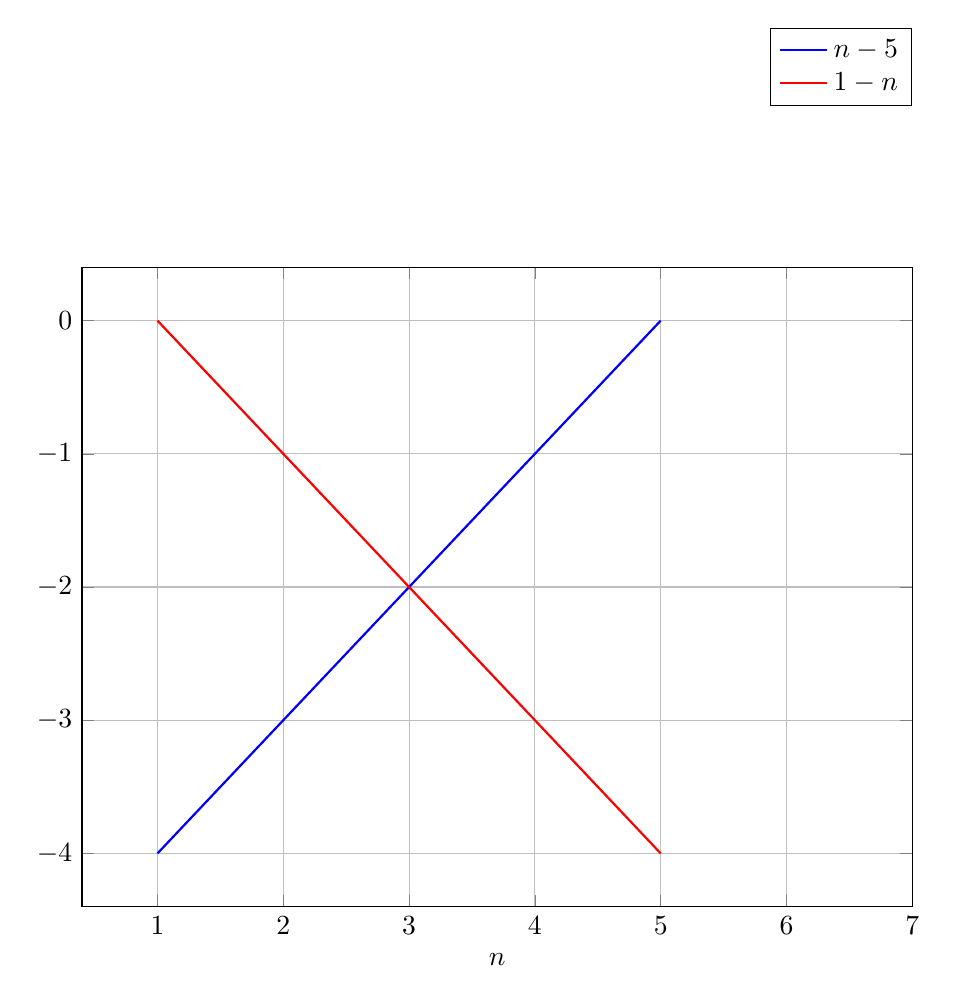
\begin{tikzpicture}
			\begin{axis}[
					xlabel={$n$},
					legend style={at={(axis cs:7,2.2)},anchor=north east},
					grid=major,
					width=\textwidth,
					height=0.8\textwidth,
					xmax=7,
				]
				\addplot[domain=1:5, samples=100, thick, blue] {x-5};
				\addplot[domain=1:5, samples=100, thick, red] {1-x};
				\legend{$n - 5$, $1-n$}
			\end{axis}
		\end{tikzpicture}
		\caption{Negative Distance to Road Boundaries}
		\label{fig:road_boundaries}
	\end{subfigure}
	\hfill
	\begin{subfigure}{0.48\textwidth}
		\centering
		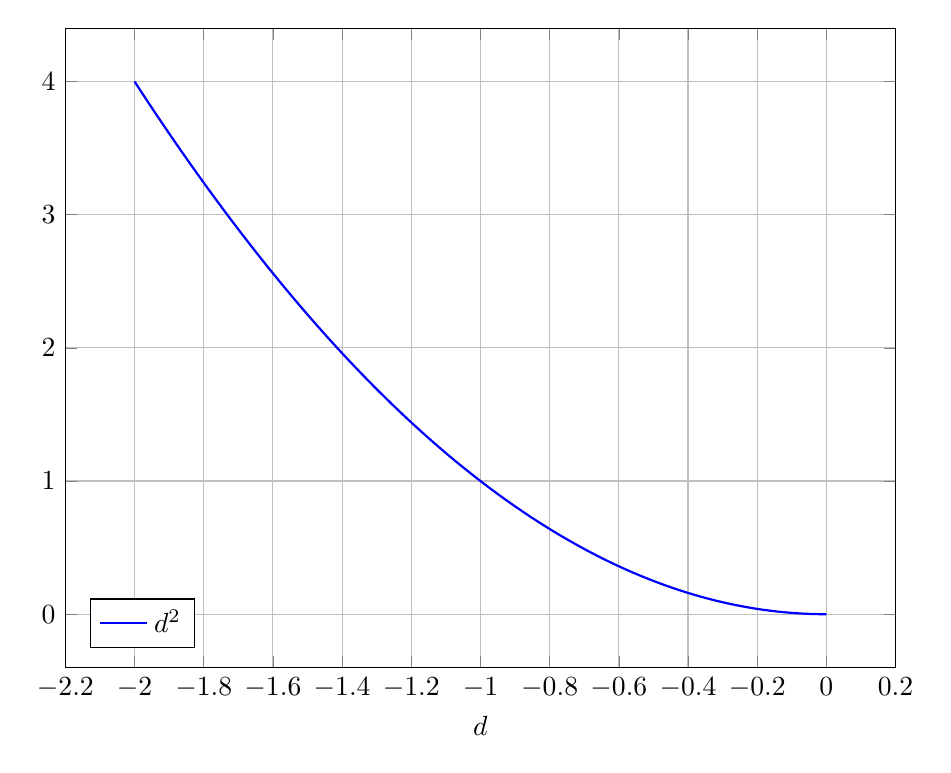
\begin{tikzpicture}
			\begin{axis}[
					xlabel={$d$},
					legend pos=south west,
					grid=major,
					width=\textwidth,
					height=0.8\textwidth
				]
				\addplot[domain=-2:0, samples=100, thick, blue] {x^2};
				\legend{$d^2$}
			\end{axis}
		\end{tikzpicture}
		\caption{Objective Function}
		\label{fig:objective_functions}
	\end{subfigure}
	\caption{Plots the distance to the road boundaries and the objective function.}
	\label{fig:auxiliary_variables}
\end{figure}

While \(\max(x-5, 1-x)\) is a convex function, it is piecewise linear, which can lead to difficulties in optimization.
The benefit of using an auxiliary variable in this context is that it allows us to transform a piecewise linear and potentially non-differentiable
objective function into a smooth and differentiable convex function.
This transformation simplifies the optimization process, making it more efficient and reliable.
Specifically, by introducing the auxiliary variable \( d \) and reformulating the objective as \(\min g(x, u) + d^2\), we obtain a function that is
easier to handle with gradient-based optimization algorithms, which rely on smoothness and differentiability to find optimal solutions effectively.

\subsection{Scenarios} \label{subsec:scenarios}

In order to evaluate the performance of our trajectory planner, we implemented several driving scenarios.
These scenarios are designed to test different aspects of the planner's capabilities.
The Straight Road scenario evaluates the planner's ability to maintain a straight path with minimal control effort, ensuring smooth and efficient
driving.
In the Left Turn scenario, the planner's performance is assessed based on its ability to execute a smooth left turn while adhering to the reference
trajectory.
The Lane Change scenario tests the planner's capability to perform a lane change maneuver safely and efficiently, highlighting its responsiveness and
precision.
The Slalom scenario challenges the planner to navigate through a series of closely spaced obstacles, requiring precise control and smooth transitions
between maneuvers.
The Elchtest, also known as the moose test, evaluates the planner's ability to perform a sudden evasive maneuver to avoid an obstacle, testing its
quick decision-making and control under pressure.
The Elchtest scenario can be visualized as follows:
\begin{figure}[H]
	\centering
	\begin{tikzpicture}
		\draw[thick, dashed] (0,-0.5) -- (5,-0.5); % Road boundary
		\draw[thick, dashed] (0,0.5) -- (3,0.5); % Road boundary
		\draw[thick, dashed] (3,0.5) -- (3,1.5); % Road boundary
		\draw[thick, dashed] (5,0.5) -- (5,-0.5); % Road boundary
		\draw[thick, dashed] (5,0.5) -- (7,0.5); % Road boundary
		\draw[thick, dashed] (3,1.5) -- (9,1.5); % Road boundary
		\draw[thick, dashed] (9,0.5) -- (9,1.5); % Road boundary
		\draw[thick, dashed] (7,0.5) -- (7,-0.5); % Road boundary
		\draw[thick, dashed] (7,-0.5) -- (12,-0.5); % Road boundary
		\draw[thick, dashed] (9,0.5) -- (12,0.5); % Road boundary
		\node at (0,0) {Start};
		\node at (12,0) {End};
	\end{tikzpicture}
	\caption{Elchtest scenario visualization}
	\label{fig:elchtest}
\end{figure}

Finally, the Sharp U Turn scenario tests the planner's ability to execute a sharp U-turn, challenging its control effort and adherence to the desired
terminal state.

By evaluating the planner in these diverse scenarios, we can gain a comprehensive understanding of its strengths and areas for improvement.

\begin{longtable}{l c c c c c}
	\caption{Overview of Road Segments and Their Properties}                                                                                             \\
	\toprule
	\textbf{Road Name}                & \textbf{Segment} & \textbf{Length} & \textbf{Curvature} & \multicolumn{2}{c}{\textbf{Lane Width}}                \\
	\cmidrule(lr){5-6}
	                                  &                  &                 &                    & \textbf{Start}                          & \textbf{End} \\
	\midrule
	\endfirsthead

	\multicolumn{6}{c}{\textit{Continued from previous page}}                                                                                            \\
	\toprule
	\textbf{Road Name}                & \textbf{Segment} & \textbf{Length} & \textbf{Curvature} & \multicolumn{2}{c}{\textbf{Lane Width}}                \\
	\cmidrule(lr){5-6}
	                                  &                  &                 &                    & \textbf{Start}                          & \textbf{End} \\
	\midrule
	\endhead

	\bottomrule
	\multicolumn{6}{c}{\textit{Continued on next page}}                                                                                                  \\
	\endfoot

	\bottomrule
	\endlastfoot

	\multirow{5}{*}{Elchtest}         & 1                & 12.0            & 0.000              & [-1.0,1.0]                              & [-1.0,1.0]   \\
	                                  & 2                & 13.5            & 0.000              & [-1.0,1.0]                              & [2.0,4.7]    \\
	                                  & 3                & 11.0            & 0.000              & [2.0,4.7]                               & [2.0,4.7]    \\
	                                  & 4                & 12.5            & 0.000              & [2.0,4.7]                               & [-1.0,1.0]   \\
	                                  & 5                & 12.0            & 0.000              & [-1.0,1.0]                              & [-1.0,1.0]   \\
	\midrule
	\multirow{1}{*}{Left Turn}        & 1                & 235.6           & 0.007              & [-2.0,2.0]                              & [-2.0,2.0]   \\
	\midrule
	\multirow{1}{*}{Straight}         & 1                & 180.0           & 0.000              & [-2.0,2.0]                              & [-2.0,2.0]   \\
	\midrule
	\multirow{4}{*}{Lane Change}      & 1                & 30.0            & 0.000              & [-2.0,2.0]                              & [-2.0,2.0]   \\
	                                  & 2                & 20.9            & 0.025              & [-2.0,2.0]                              & [-2.0,2.0]   \\
	                                  & 3                & 20.9            & -0.025             & [-2.0,2.0]                              & [-2.0,2.0]   \\
	                                  & 4                & 30.0            & 0.000              & [-2.0,2.0]                              & [-2.0,2.0]   \\
	\midrule
	\multirow{5}{*}{Slalom}           & 1                & 20.0            & 0.000              & [-2.0,2.0]                              & [-2.0,2.0]   \\
	                                  & 2                & 94.2            & -0.033             & [-2.0,2.0]                              & [-2.0,2.0]   \\
	                                  & 3                & 94.2            & 0.033              & [-2.0,2.0]                              & [-2.0,2.0]   \\
	                                  & 4                & 94.2            & -0.033             & [-2.0,2.0]                              & [-2.0,2.0]   \\
	                                  & 5                & 20.0            & 0.000              & [-2.0,2.0]                              & [-2.0,2.0]   \\
	\midrule
	\multirow{3}{*}{Feasible Curve}   & 1                & 20.0            & 0.000              & [-2.0,2.0]                              & [-2.0,2.0]   \\
	                                  & 2                & 15.7            & 0.200              & [-2.0,2.0]                              & [-2.0,2.0]   \\
	                                  & 3                & 20.0            & 0.000              & [-2.0,2.0]                              & [-2.0,2.0]   \\
	\midrule
	\multirow{3}{*}{Infeasible Curve} & 1                & 20.0            & 0.000              & [-2.0,2.0]                              & [-2.0,2.0]   \\
	                                  & 2                & 8.8             & 0.357              & [-2.0,2.0]                              & [-2.0,2.0]   \\
	                                  & 3                & 20.0            & 0.000              & [-2.0,2.0]                              & [-2.0,2.0]   \\
	\midrule
	\label{tab:road_segments}
\end{longtable}

Table \ref{tab:road_segments} provides an overview of the road segments used in our evaluation scenarios.
Each segment is characterized by its length, curvature, and lane width at the start and end points.
This detailed breakdown helps in understanding the specific challenges posed by each scenario and how the trajectory planner adapts to different road
conditions.

\subsection{Simulation Setup} \label{subsec:simulation}

For the vehicle simulation, we employ a more sophisticated model from \cite{noauthor_dateien_2021} and discretize its dynamics using the Runge-Kutta
method \cite{griffiths_rungekutta_2010}, which offers greater accuracy compared to the forward Euler method used for trajectory planning.
To ensure reproducibility, we define the model using the following state variables and control inputs: \[ x = [p_x, p_y, \delta, v, \psi, \dot{\psi},
	\beta]^T, u = [a_x, v_{\delta}]^T \] where $p_x$, $p_y$ represent the vehicle's position coordinates, $\delta$ is the steering angle, $v$ is the
velocity, $\psi$ is the yaw angle, $\dot{\psi}$ is the yaw rate, $\beta$ is the slip angle, $a_x$ is the longitudinal acceleration, and $v_\delta$ is
the steering rate.

The model's dynamics are governed by the following equations, valid for $|v|\geq0.1$:
\[
	f(x, u) = \begin{bmatrix}
		v\cos(\psi + \beta)                                  \\
		v\sin(\psi + \beta)                                  \\
		v_\delta                                             \\
		a_x                                                  \\
		\dot{\psi}                                           \\
		\frac{\mu\,m}{I_{z}(l_{r}+l_{f})}\Bigl(
		l_{f}\,C_{S,f}\bigl(g\,l_{r}-a_xh_{cg}\bigr)\,\delta \\
		\;+                                                 \;\bigl[l_{r}\,C_{S,r}\bigl(g\,l_{f}+a_xh_{cg}\bigr)
			\;-\;l_{f}\,C_{S,f}\bigl(g\,l_{r}-a_xh_{cg}\bigr)\bigr]\,\beta
		\Bigr)                                               \\
		\quad -\;\Bigl[
		l_{f}^{2}\,C_{S,f}\bigl(g\,l_{r}-a_xh_{cg}\bigr)
		\;+\;
		l_{r}^{2}\,C_{S,r}\bigl(g\,l_{f}+a_xh_{cg}\bigr)
		\Bigr]
		\frac{\dot{\psi}}{v}                                 \\
		\frac{\mu}{v\,\bigl(l_{r}+l_{f}\bigr)}\Bigl(
		C_{S,f}\bigl(g\,l_{r}-a_xh_{cg}\bigr)\,\delta
		\;-\;
		\bigl[C_{S,r}\bigl(g\,l_{f}+a_xh_{cg}\bigr)          \\
			\;+\;
		C_{S,f}\bigl(g\,l_{r}-a_xh_{cg}\bigr)\bigr]\,\beta   \\
		\quad +\;\bigl[
			C_{S,r}\bigl(g\,l_{f}+a_xh_{cg}\bigr)\,l_{r}
			\;-\;
			C_{S,f}\bigl(g\,l_{r}-a_xh_{cg}\bigr)\,l_{f}
			\bigr]
		\frac{\dot{\psi}}{v}
		\Bigr)
		\;-\;
		\dot{\psi}
	\end{bmatrix}
\]
For smaller velocities $|v|<0.1$, the dynamics simplify to:
\[
	f(x, u) = \begin{bmatrix}
		v\cos(\psi + \beta) \\
		v\sin(\psi + \beta) \\
		v_\delta            \\
		a_x                 \\
		\dot{\psi}          \\
		\frac{1}{l_{wb}}
		\biggl(
		a_x\,\cos( \beta)\,\tan(\delta)
		\;-\;
		v\,\sin( \beta)\,\tan(\delta)\,\dot{x}_{7}
		\;+\;
		\frac{v\,\cos( \beta)}{\cos^2(\delta)}\,
		v_{\delta}
		\biggr)
		\\
		\frac{1}{1 +
			\bigl(\tan(\delta)\tfrac{l_{r}}{l_{wb}}\bigr)^2}
		\;\cdot\;
		\frac{l_{r}}{l_{wb}\,\cos^2(\delta)}\,
		v_{\delta}
	\end{bmatrix}
\]

We consider a vehicle, with the identifier '1' from \cite{noauthor_dateien_2021} of length \(l = 4.298\,\mathrm{m}\) and width \(w =
1.674\,\mathrm{m}\), with total mass \(m = 1.225\times10^3\,\mathrm{kg}\) and moment of inertia \(I_z = 1.538\times10^3\,\mathrm{kg\,m}^2\).
The center of gravity is located \(l_f = 0.883\,\mathrm{m}\) from the front axle and \(l_r = 1.508\,\mathrm{m}\) from the rear axle, at a height
\(h_{cg} = 0.557\,\mathrm{m}\).
The front and rear cornering stiffness coefficients are both \(C_{S,f} = C_{S,r} = 20.89\,\text{[1/rad]}\), and the friction coefficient is \(\mu =
1.048\).
The switching velocity for the dynamics is set to \(v_S = 4.755\,\mathrm{m/s}\).

\subsection{Results}
\label{subsec:results}

Throughout our simulations, we defined specific ranges for the control inputs to ensure realistic vehicle behavior.
The longitudinal acceleration, $a_x$, was constrained within $[-6, 3]$ m/s², while the steering rate, $v_\delta$, was limited to $[-0.5, 0.5]$ rad/s.
Additionally, the steering angle, $\delta$, was bounded within $[-0.698, 0.698]$ radians.
\[
	a_x \in [-6, 3] \text{ m/s²}, \quad v_\delta \in [-0.5, 0.5] \text{ rad/s}, \quad \delta \in [-0.698, 0.698] \text{ rad}
\]
To evaluate performance under different conditions, we simulated all scenarios at three distinct speeds:
\[
	v_{low}=5 \text{m/s}, v_{mid}=10 \text{m/s}, \text{and } v_{high}=20 \text{m/s}.
\]
We also allowed the vehicle to decelerate down to $70\%$ of its initial speed.

For time discretization, we implemented two configurations, represented as \[ t_{\text{conf}} = (T, R, \Delta t, \Delta^2 t_{\text{replan}}) \] where
$T$ is the time horizon, $R$ is the replanning interval, the initial constant time interval $\Delta t$ for the first few time points, and the
increasing time interval $\Delta^2 t_{\text{replan}}$ for the remaining time points as illustrated in \ref{fig:time_points}.
The first configuration, $t_{\text{conf}}^{(1)}$, was set to a smaller time horizon with a finer $\Delta t$, while the second configuration,
$t_{\text{conf}}^{(2)}$, used a larger time horizon with a coarser $\Delta t$ as well as a smaller slope for the time steps after the replanning
interval, providing two distinct approaches for evaluating planning and control strategies.
\begin{align*}
	t_{\text{conf}}^{(1)} = (3\text{s}, 0.1\text{s}, 10\text{ms}, 40\text{ms}) \\
	t_{\text{conf}}^{(2)} = (5\text{s}, 0.1\text{s}, 20\text{ms}, 20\text{ms})
\end{align*}

We used four objectives to evaluate performance: the control effort cost $J_{control}$, the trajectory tracking cost $J_{tracking}$, the terminal
cost $J_{terminal}$, and the combined cost function $J$ from \eqref{eq:cost_function_combined}, with weighting factors $\alpha = 1$, $\beta = 10^3$,
and $\gamma = 10^4$.
Those weights were chosen to equally balance the objectives.
\[
	J_{control}, J_{tracking}, J_{terminal}, J
\]

All simulations were conducted on a MacBook Air equipped with an Apple M1 processor and 16 GB of unified memory.
The operating system used was macOS 15.3 (24D60).
The simulations were executed using Python 3.11.3, compiled with Clang 13.0.0.

\subsubsection{Solver Times}

This section evaluates solver performance across different models and configurations.
We assessed efficiency by running simulations with varying velocity, scenarios, and objective functions, totaling $96$ simulations per
model-configuration pair.

Table \ref{tab:solver_performance} summarizes the average solver time and its deviation for each model and configuration.

\begin{table}[h]
	\centering
	\caption{Solver Performance for Different Models and Configurations}
	\label{tab:solver_performance}
	\begin{tabular}{lcccc}
		\toprule
		\textbf{Model}    & \textbf{Configuration}  & \textbf{Avg Time (ms)} & \textbf{Time Deviation (ms)} \\
		\midrule
		Double Integrator & $t_{\text{conf}}^{(1)}$ & 3.9                    & 1.0                          \\
		Double Integrator & $t_{\text{conf}}^{(2)}$ & 3.8                    & 1.3                          \\
		Bicycle           & $t_{\text{conf}}^{(1)}$ & 9.5                    & 2.1                          \\
		Bicycle           & $t_{\text{conf}}^{(2)}$ & 9.4                    & 2.9                          \\
		\bottomrule
	\end{tabular}
\end{table}

The double integrator model outperforms the bicycle model, achieving solver times of $3.9$ms and $3.8$ms across both configurations.
In contrast, the bicycle model requires $9.5$ms and $9.4$ms, making it over twice as slow.
Solver time deviations also differ significantly: the double integrator model exhibits deviations of $1.0$ms and $1.3$ms, while the bicycle model
experiences deviations of $2.1$ms and $2.9$ms.

This indicates that the double integrator model provides not only faster solutions but also more stable performance.

\begin{figure}[h!]
	\centering
	\resizebox{\textwidth}{!}{
		\begin{adjustbox}{clip, trim=0cm 0cm 0cm 9.8cm} % left, bottom, right, top
			\input{../code/benchmark-results/slalom-PointMassModel-44e48f14-d19d-4b3f-b484-f84f67a1bcf5/solver_metrics.pgf}
		\end{adjustbox}
	}
	\caption{Solver metrics for Slalom scenario using double integrator model}
	\label{fig:slalom_point_mass_model}
\end{figure}

\begin{figure}[h!]
	\centering
	\resizebox{\textwidth}{!}{
		\begin{adjustbox}{clip, trim=0cm 0cm 0cm 10cm} % left, bottom, right, top
			\input{../code/benchmark-results/slalom-BicycleModel-f33181f3-900a-45bf-88f1-ebadf0bf8a1e/solver_metrics.pgf}
		\end{adjustbox}
	}
	\caption{Solver metrics for Slalom scenario using kinematic bicycle model}
	\label{fig:slalom_bicycle_model}
\end{figure}

Figures \ref{fig:slalom_point_mass_model} and \ref{fig:slalom_bicycle_model} illustrate solver performance in the Slalom scenario.
\begin{itemize}
	\item The double integrator model maintains relatively stable solver times across iterations.
	\item The bicycle model exhibits more variation, aligning with the larger solver time deviations observed in Table \ref{tab:solver_performance}.
\end{itemize}

These findings confirm that the double integrator model provides a more consistent and efficient solution.

\subsubsection{Completion Rates}

Figure \ref{fig:failed_scenarios} presents the number of failed scenarios per model.
As expected, both models fail every test in the Infeasible Curve scenario, which is intentionally designed to be unsolvable.
However, when the curve radius increases slightly (making the scenario marginally feasible), both models successfully complete it at the lowest
velocity $v_{\text{low}}$.

\begin{figure}[h]
	\centering
	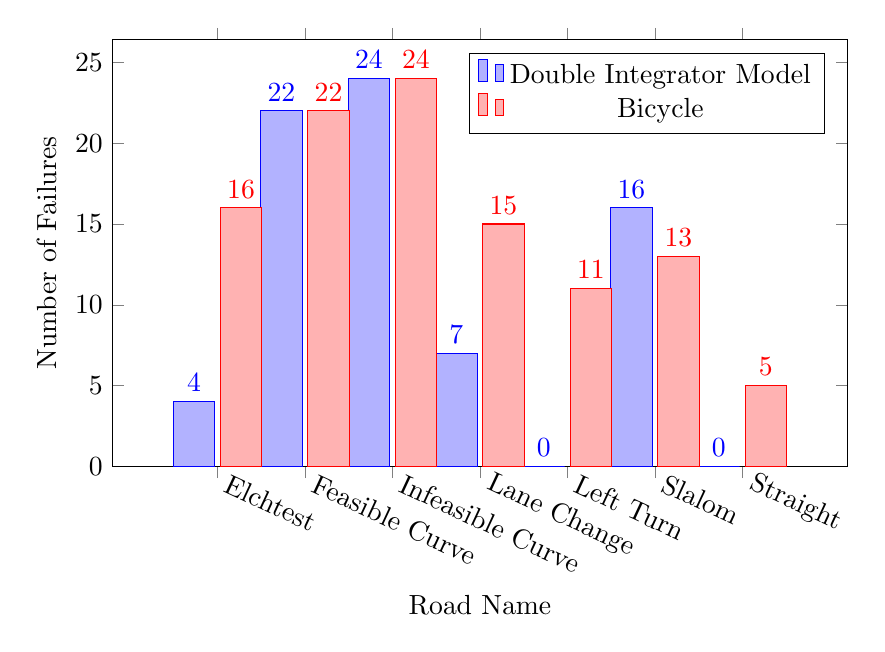
\begin{tikzpicture}
		\begin{axis}[
				ybar,
				bar width=15pt, % Increase bar width
				width=0.9\textwidth, % Increase overall figure width
				height=7cm,
				enlarge x limits=0.2, % Add some space on both sides
				symbolic x coords={Elchtest, Feasible Curve, Infeasible Curve, Lane Change, Left Turn, Slalom, Straight}, % Replace with actual road names
				xtick=data,
				xticklabel style={rotate=-25, anchor=west}, % Rotate labels for readability
				ymin=0,
				ylabel={Number of Failures},
				xlabel={Road Name},
				legend pos=north east,
				nodes near coords
			]
			% Replace the values below with actual failure counts
			\addplot coordinates {(Elchtest,4) (Feasible Curve,22) (Infeasible Curve,24) (Lane Change,7) (Left Turn,0) (Slalom,16) (Straight,0)};
			\addlegendentry{Double Integrator Model}

			\addplot coordinates {(Elchtest,16) (Feasible Curve,22) (Infeasible Curve,24) (Lane Change,15) (Left Turn,11) (Slalom,13) (Straight,5)};
			\addlegendentry{Bicycle}
		\end{axis}
	\end{tikzpicture}
	\caption{Histogram of Failed Scenarios per Model}
	\label{fig:failed_scenarios}
\end{figure}

The results indicate that higher speeds lead to higher failure rates.
However, an anomaly occurs in the Straight scenario, where the bicycle model has a higher failure rate at lower velocities.
This issue arises when using the $J_{\text{terminal}}$ objective function, which prioritizes velocity maximization.
This suggests a numerical instability that may be resolved using soft constraints.

\begin{figure}[h]
	\centering
	\begin{tikzpicture}
		\begin{groupplot}[
				group style={group size=2 by 1, horizontal sep=2cm}, % Two plots side by side
				width=0.5\textwidth, % Adjust width for each plot
				height=7cm,
				symbolic x coords={Elchtest, Feasible Curve, Lane Change, Left Turn, Slalom, Straight}, % Road names
				xtick=data,
				xticklabel style={rotate=-45, anchor=west}, % Rotate labels for readability
				ymin=0,
				ylabel={Number of Failures},
				xlabel={Road Name},
			]

			\nextgroupplot[
				title={Double Integrator Model},
				ybar stacked, % Stacked bars
				bar width=15pt, % Moved inside the groupplot
				nodes near coords, % Show numbers on bars
				every node near coord/.append style={yshift=-1pt}, % Move numbers slightly down
			]
			\addplot coordinates { (Elchtest, 0) (Feasible Curve, 6) (Lane Change, 0) (Left Turn, 0) (Slalom, 8) (Straight, 0) };
			\addplot coordinates { (Elchtest, 0) (Feasible Curve, 8) (Lane Change, 0) (Left Turn, 0) (Slalom, 0) (Straight, 0) };
			\addplot coordinates { (Elchtest, 4) (Feasible Curve, 8) (Lane Change, 7) (Left Turn, 0) (Slalom, 8) (Straight, 0) };
			\legend{5 m/s, 10 m/s, 20 m/s}

			% Second plot: Bicycle Model
			\nextgroupplot[
				title={Kinematic Bicycle Model},
				ybar stacked, % Stacked bars
				bar width=15pt, % Moved inside the groupplot
				nodes near coords, % Show numbers on bars
				every node near coord/.append style={yshift=-1pt}, % Move numbers slightly down
			]
			\addplot coordinates { (Elchtest, 3) (Feasible Curve, 6) (Lane Change, 3) (Left Turn, 2) (Slalom, 3) (Straight, 2) };
			\addplot coordinates { (Elchtest, 5) (Feasible Curve, 8) (Lane Change, 5) (Left Turn, 4) (Slalom, 5) (Straight, 2) };
			\addplot coordinates { (Elchtest, 8) (Feasible Curve, 8) (Lane Change, 7) (Left Turn, 5) (Slalom, 5) (Straight, 1) };
			\legend{5 m/s, 10 m/s, 20 m/s}
		\end{groupplot}
	\end{tikzpicture}
	\caption{Stacked Histogram of Failed Road Names per Model with Velocity}
	\label{fig:failed_scenarios_stacked}
\end{figure}

The bicycle model completes more runs in the slalom scenario compared to the double integrator model.
This is because the double integrator model considers the worst-case scenario and does not find a solution if it is infeasible to drive on the inner
side of the curve, even though it might be feasible to drive on the outer line.
For example driving at the highest speed $v_{max}$, the resulting polytope of the double integrator model is empty.
Limiting the vehicle options to the outer side and reduce the upper speed limit to $14.5$m/s results in a non-empty set.
In fact, we can observe that the bicycle model completes the slalom always at the outer lines (see \ref{fig:slalom_bicycle_model_n}), while driving
at around $14.5$m/s (see \ref{fig:slalom_bicycle_model_velocity}).

\begin{figure}[h!]
	\centering
	\resizebox{\textwidth}{!}{
		\begin{adjustbox}{clip, trim=0cm 14.5cm 0cm 4.8cm}
			%% Creator: Matplotlib, PGF backend
%%
%% To include the figure in your LaTeX document, write
%%   \input{<filename>.pgf}
%%
%% Make sure the required packages are loaded in your preamble
%%   \usepackage{pgf}
%%
%% Also ensure that all the required font packages are loaded; for instance,
%% the lmodern package is sometimes necessary when using math font.
%%   \usepackage{lmodern}
%%
%% Figures using additional raster images can only be included by \input if
%% they are in the same directory as the main LaTeX file. For loading figures
%% from other directories you can use the `import` package
%%   \usepackage{import}
%%
%% and then include the figures with
%%   \import{<path to file>}{<filename>.pgf}
%%
%% Matplotlib used the following preamble
%%   \def\mathdefault#1{#1}
%%   \everymath=\expandafter{\the\everymath\displaystyle}
%%   
%%   \ifdefined\pdftexversion\else  % non-pdftex case.
%%     \usepackage{fontspec}
%%   \fi
%%   \makeatletter\@ifpackageloaded{underscore}{}{\usepackage[strings]{underscore}}\makeatother
%%
\begingroup%
\makeatletter%
\begin{pgfpicture}%
\pgfpathrectangle{\pgfpointorigin}{\pgfqpoint{9.861316in}{7.457149in}}%
\pgfusepath{use as bounding box, clip}%
\begin{pgfscope}%
\pgfsetbuttcap%
\pgfsetmiterjoin%
\definecolor{currentfill}{rgb}{1.000000,1.000000,1.000000}%
\pgfsetfillcolor{currentfill}%
\pgfsetlinewidth{0.000000pt}%
\definecolor{currentstroke}{rgb}{1.000000,1.000000,1.000000}%
\pgfsetstrokecolor{currentstroke}%
\pgfsetdash{}{0pt}%
\pgfpathmoveto{\pgfqpoint{0.000000in}{0.000000in}}%
\pgfpathlineto{\pgfqpoint{9.861316in}{0.000000in}}%
\pgfpathlineto{\pgfqpoint{9.861316in}{7.457149in}}%
\pgfpathlineto{\pgfqpoint{0.000000in}{7.457149in}}%
\pgfpathlineto{\pgfqpoint{0.000000in}{0.000000in}}%
\pgfpathclose%
\pgfusepath{fill}%
\end{pgfscope}%
\begin{pgfscope}%
\pgfsetbuttcap%
\pgfsetmiterjoin%
\definecolor{currentfill}{rgb}{1.000000,1.000000,1.000000}%
\pgfsetfillcolor{currentfill}%
\pgfsetlinewidth{0.000000pt}%
\definecolor{currentstroke}{rgb}{0.000000,0.000000,0.000000}%
\pgfsetstrokecolor{currentstroke}%
\pgfsetstrokeopacity{0.000000}%
\pgfsetdash{}{0pt}%
\pgfpathmoveto{\pgfqpoint{0.716279in}{6.092222in}}%
\pgfpathlineto{\pgfqpoint{9.761316in}{6.092222in}}%
\pgfpathlineto{\pgfqpoint{9.761316in}{7.357149in}}%
\pgfpathlineto{\pgfqpoint{0.716279in}{7.357149in}}%
\pgfpathlineto{\pgfqpoint{0.716279in}{6.092222in}}%
\pgfpathclose%
\pgfusepath{fill}%
\end{pgfscope}%
\begin{pgfscope}%
\pgfsetbuttcap%
\pgfsetroundjoin%
\definecolor{currentfill}{rgb}{0.000000,0.000000,0.000000}%
\pgfsetfillcolor{currentfill}%
\pgfsetlinewidth{0.803000pt}%
\definecolor{currentstroke}{rgb}{0.000000,0.000000,0.000000}%
\pgfsetstrokecolor{currentstroke}%
\pgfsetdash{}{0pt}%
\pgfsys@defobject{currentmarker}{\pgfqpoint{0.000000in}{-0.048611in}}{\pgfqpoint{0.000000in}{0.000000in}}{%
\pgfpathmoveto{\pgfqpoint{0.000000in}{0.000000in}}%
\pgfpathlineto{\pgfqpoint{0.000000in}{-0.048611in}}%
\pgfusepath{stroke,fill}%
}%
\begin{pgfscope}%
\pgfsys@transformshift{1.127417in}{6.092222in}%
\pgfsys@useobject{currentmarker}{}%
\end{pgfscope}%
\end{pgfscope}%
\begin{pgfscope}%
\definecolor{textcolor}{rgb}{0.000000,0.000000,0.000000}%
\pgfsetstrokecolor{textcolor}%
\pgfsetfillcolor{textcolor}%
\pgftext[x=1.127417in,y=5.995000in,,top]{\color{textcolor}{\rmfamily\fontsize{9.000000}{10.800000}\selectfont\catcode`\^=\active\def^{\ifmmode\sp\else\^{}\fi}\catcode`\%=\active\def%{\%}$\mathdefault{0}$}}%
\end{pgfscope}%
\begin{pgfscope}%
\pgfsetbuttcap%
\pgfsetroundjoin%
\definecolor{currentfill}{rgb}{0.000000,0.000000,0.000000}%
\pgfsetfillcolor{currentfill}%
\pgfsetlinewidth{0.803000pt}%
\definecolor{currentstroke}{rgb}{0.000000,0.000000,0.000000}%
\pgfsetstrokecolor{currentstroke}%
\pgfsetdash{}{0pt}%
\pgfsys@defobject{currentmarker}{\pgfqpoint{0.000000in}{-0.048611in}}{\pgfqpoint{0.000000in}{0.000000in}}{%
\pgfpathmoveto{\pgfqpoint{0.000000in}{0.000000in}}%
\pgfpathlineto{\pgfqpoint{0.000000in}{-0.048611in}}%
\pgfusepath{stroke,fill}%
}%
\begin{pgfscope}%
\pgfsys@transformshift{2.739723in}{6.092222in}%
\pgfsys@useobject{currentmarker}{}%
\end{pgfscope}%
\end{pgfscope}%
\begin{pgfscope}%
\definecolor{textcolor}{rgb}{0.000000,0.000000,0.000000}%
\pgfsetstrokecolor{textcolor}%
\pgfsetfillcolor{textcolor}%
\pgftext[x=2.739723in,y=5.995000in,,top]{\color{textcolor}{\rmfamily\fontsize{9.000000}{10.800000}\selectfont\catcode`\^=\active\def^{\ifmmode\sp\else\^{}\fi}\catcode`\%=\active\def%{\%}$\mathdefault{1}$}}%
\end{pgfscope}%
\begin{pgfscope}%
\pgfsetbuttcap%
\pgfsetroundjoin%
\definecolor{currentfill}{rgb}{0.000000,0.000000,0.000000}%
\pgfsetfillcolor{currentfill}%
\pgfsetlinewidth{0.803000pt}%
\definecolor{currentstroke}{rgb}{0.000000,0.000000,0.000000}%
\pgfsetstrokecolor{currentstroke}%
\pgfsetdash{}{0pt}%
\pgfsys@defobject{currentmarker}{\pgfqpoint{0.000000in}{-0.048611in}}{\pgfqpoint{0.000000in}{0.000000in}}{%
\pgfpathmoveto{\pgfqpoint{0.000000in}{0.000000in}}%
\pgfpathlineto{\pgfqpoint{0.000000in}{-0.048611in}}%
\pgfusepath{stroke,fill}%
}%
\begin{pgfscope}%
\pgfsys@transformshift{4.352029in}{6.092222in}%
\pgfsys@useobject{currentmarker}{}%
\end{pgfscope}%
\end{pgfscope}%
\begin{pgfscope}%
\definecolor{textcolor}{rgb}{0.000000,0.000000,0.000000}%
\pgfsetstrokecolor{textcolor}%
\pgfsetfillcolor{textcolor}%
\pgftext[x=4.352029in,y=5.995000in,,top]{\color{textcolor}{\rmfamily\fontsize{9.000000}{10.800000}\selectfont\catcode`\^=\active\def^{\ifmmode\sp\else\^{}\fi}\catcode`\%=\active\def%{\%}$\mathdefault{2}$}}%
\end{pgfscope}%
\begin{pgfscope}%
\pgfsetbuttcap%
\pgfsetroundjoin%
\definecolor{currentfill}{rgb}{0.000000,0.000000,0.000000}%
\pgfsetfillcolor{currentfill}%
\pgfsetlinewidth{0.803000pt}%
\definecolor{currentstroke}{rgb}{0.000000,0.000000,0.000000}%
\pgfsetstrokecolor{currentstroke}%
\pgfsetdash{}{0pt}%
\pgfsys@defobject{currentmarker}{\pgfqpoint{0.000000in}{-0.048611in}}{\pgfqpoint{0.000000in}{0.000000in}}{%
\pgfpathmoveto{\pgfqpoint{0.000000in}{0.000000in}}%
\pgfpathlineto{\pgfqpoint{0.000000in}{-0.048611in}}%
\pgfusepath{stroke,fill}%
}%
\begin{pgfscope}%
\pgfsys@transformshift{5.964335in}{6.092222in}%
\pgfsys@useobject{currentmarker}{}%
\end{pgfscope}%
\end{pgfscope}%
\begin{pgfscope}%
\definecolor{textcolor}{rgb}{0.000000,0.000000,0.000000}%
\pgfsetstrokecolor{textcolor}%
\pgfsetfillcolor{textcolor}%
\pgftext[x=5.964335in,y=5.995000in,,top]{\color{textcolor}{\rmfamily\fontsize{9.000000}{10.800000}\selectfont\catcode`\^=\active\def^{\ifmmode\sp\else\^{}\fi}\catcode`\%=\active\def%{\%}$\mathdefault{3}$}}%
\end{pgfscope}%
\begin{pgfscope}%
\pgfsetbuttcap%
\pgfsetroundjoin%
\definecolor{currentfill}{rgb}{0.000000,0.000000,0.000000}%
\pgfsetfillcolor{currentfill}%
\pgfsetlinewidth{0.803000pt}%
\definecolor{currentstroke}{rgb}{0.000000,0.000000,0.000000}%
\pgfsetstrokecolor{currentstroke}%
\pgfsetdash{}{0pt}%
\pgfsys@defobject{currentmarker}{\pgfqpoint{0.000000in}{-0.048611in}}{\pgfqpoint{0.000000in}{0.000000in}}{%
\pgfpathmoveto{\pgfqpoint{0.000000in}{0.000000in}}%
\pgfpathlineto{\pgfqpoint{0.000000in}{-0.048611in}}%
\pgfusepath{stroke,fill}%
}%
\begin{pgfscope}%
\pgfsys@transformshift{7.576641in}{6.092222in}%
\pgfsys@useobject{currentmarker}{}%
\end{pgfscope}%
\end{pgfscope}%
\begin{pgfscope}%
\definecolor{textcolor}{rgb}{0.000000,0.000000,0.000000}%
\pgfsetstrokecolor{textcolor}%
\pgfsetfillcolor{textcolor}%
\pgftext[x=7.576641in,y=5.995000in,,top]{\color{textcolor}{\rmfamily\fontsize{9.000000}{10.800000}\selectfont\catcode`\^=\active\def^{\ifmmode\sp\else\^{}\fi}\catcode`\%=\active\def%{\%}$\mathdefault{4}$}}%
\end{pgfscope}%
\begin{pgfscope}%
\pgfsetbuttcap%
\pgfsetroundjoin%
\definecolor{currentfill}{rgb}{0.000000,0.000000,0.000000}%
\pgfsetfillcolor{currentfill}%
\pgfsetlinewidth{0.803000pt}%
\definecolor{currentstroke}{rgb}{0.000000,0.000000,0.000000}%
\pgfsetstrokecolor{currentstroke}%
\pgfsetdash{}{0pt}%
\pgfsys@defobject{currentmarker}{\pgfqpoint{0.000000in}{-0.048611in}}{\pgfqpoint{0.000000in}{0.000000in}}{%
\pgfpathmoveto{\pgfqpoint{0.000000in}{0.000000in}}%
\pgfpathlineto{\pgfqpoint{0.000000in}{-0.048611in}}%
\pgfusepath{stroke,fill}%
}%
\begin{pgfscope}%
\pgfsys@transformshift{9.188947in}{6.092222in}%
\pgfsys@useobject{currentmarker}{}%
\end{pgfscope}%
\end{pgfscope}%
\begin{pgfscope}%
\definecolor{textcolor}{rgb}{0.000000,0.000000,0.000000}%
\pgfsetstrokecolor{textcolor}%
\pgfsetfillcolor{textcolor}%
\pgftext[x=9.188947in,y=5.995000in,,top]{\color{textcolor}{\rmfamily\fontsize{9.000000}{10.800000}\selectfont\catcode`\^=\active\def^{\ifmmode\sp\else\^{}\fi}\catcode`\%=\active\def%{\%}$\mathdefault{5}$}}%
\end{pgfscope}%
\begin{pgfscope}%
\definecolor{textcolor}{rgb}{0.000000,0.000000,0.000000}%
\pgfsetstrokecolor{textcolor}%
\pgfsetfillcolor{textcolor}%
\pgftext[x=5.238797in,y=5.828333in,,top]{\color{textcolor}{\rmfamily\fontsize{11.000000}{13.200000}\selectfont\catcode`\^=\active\def^{\ifmmode\sp\else\^{}\fi}\catcode`\%=\active\def%{\%}Time [s]}}%
\end{pgfscope}%
\begin{pgfscope}%
\pgfsetbuttcap%
\pgfsetroundjoin%
\definecolor{currentfill}{rgb}{0.000000,0.000000,0.000000}%
\pgfsetfillcolor{currentfill}%
\pgfsetlinewidth{0.803000pt}%
\definecolor{currentstroke}{rgb}{0.000000,0.000000,0.000000}%
\pgfsetstrokecolor{currentstroke}%
\pgfsetdash{}{0pt}%
\pgfsys@defobject{currentmarker}{\pgfqpoint{-0.048611in}{0.000000in}}{\pgfqpoint{-0.000000in}{0.000000in}}{%
\pgfpathmoveto{\pgfqpoint{-0.000000in}{0.000000in}}%
\pgfpathlineto{\pgfqpoint{-0.048611in}{0.000000in}}%
\pgfusepath{stroke,fill}%
}%
\begin{pgfscope}%
\pgfsys@transformshift{0.716279in}{6.149719in}%
\pgfsys@useobject{currentmarker}{}%
\end{pgfscope}%
\end{pgfscope}%
\begin{pgfscope}%
\definecolor{textcolor}{rgb}{0.000000,0.000000,0.000000}%
\pgfsetstrokecolor{textcolor}%
\pgfsetfillcolor{textcolor}%
\pgftext[x=0.554821in, y=6.106316in, left, base]{\color{textcolor}{\rmfamily\fontsize{9.000000}{10.800000}\selectfont\catcode`\^=\active\def^{\ifmmode\sp\else\^{}\fi}\catcode`\%=\active\def%{\%}$\mathdefault{0}$}}%
\end{pgfscope}%
\begin{pgfscope}%
\pgfsetbuttcap%
\pgfsetroundjoin%
\definecolor{currentfill}{rgb}{0.000000,0.000000,0.000000}%
\pgfsetfillcolor{currentfill}%
\pgfsetlinewidth{0.803000pt}%
\definecolor{currentstroke}{rgb}{0.000000,0.000000,0.000000}%
\pgfsetstrokecolor{currentstroke}%
\pgfsetdash{}{0pt}%
\pgfsys@defobject{currentmarker}{\pgfqpoint{-0.048611in}{0.000000in}}{\pgfqpoint{-0.000000in}{0.000000in}}{%
\pgfpathmoveto{\pgfqpoint{-0.000000in}{0.000000in}}%
\pgfpathlineto{\pgfqpoint{-0.048611in}{0.000000in}}%
\pgfusepath{stroke,fill}%
}%
\begin{pgfscope}%
\pgfsys@transformshift{0.716279in}{6.494458in}%
\pgfsys@useobject{currentmarker}{}%
\end{pgfscope}%
\end{pgfscope}%
\begin{pgfscope}%
\definecolor{textcolor}{rgb}{0.000000,0.000000,0.000000}%
\pgfsetstrokecolor{textcolor}%
\pgfsetfillcolor{textcolor}%
\pgftext[x=0.490585in, y=6.451056in, left, base]{\color{textcolor}{\rmfamily\fontsize{9.000000}{10.800000}\selectfont\catcode`\^=\active\def^{\ifmmode\sp\else\^{}\fi}\catcode`\%=\active\def%{\%}$\mathdefault{10}$}}%
\end{pgfscope}%
\begin{pgfscope}%
\pgfsetbuttcap%
\pgfsetroundjoin%
\definecolor{currentfill}{rgb}{0.000000,0.000000,0.000000}%
\pgfsetfillcolor{currentfill}%
\pgfsetlinewidth{0.803000pt}%
\definecolor{currentstroke}{rgb}{0.000000,0.000000,0.000000}%
\pgfsetstrokecolor{currentstroke}%
\pgfsetdash{}{0pt}%
\pgfsys@defobject{currentmarker}{\pgfqpoint{-0.048611in}{0.000000in}}{\pgfqpoint{-0.000000in}{0.000000in}}{%
\pgfpathmoveto{\pgfqpoint{-0.000000in}{0.000000in}}%
\pgfpathlineto{\pgfqpoint{-0.048611in}{0.000000in}}%
\pgfusepath{stroke,fill}%
}%
\begin{pgfscope}%
\pgfsys@transformshift{0.716279in}{6.839198in}%
\pgfsys@useobject{currentmarker}{}%
\end{pgfscope}%
\end{pgfscope}%
\begin{pgfscope}%
\definecolor{textcolor}{rgb}{0.000000,0.000000,0.000000}%
\pgfsetstrokecolor{textcolor}%
\pgfsetfillcolor{textcolor}%
\pgftext[x=0.490585in, y=6.795795in, left, base]{\color{textcolor}{\rmfamily\fontsize{9.000000}{10.800000}\selectfont\catcode`\^=\active\def^{\ifmmode\sp\else\^{}\fi}\catcode`\%=\active\def%{\%}$\mathdefault{20}$}}%
\end{pgfscope}%
\begin{pgfscope}%
\pgfsetbuttcap%
\pgfsetroundjoin%
\definecolor{currentfill}{rgb}{0.000000,0.000000,0.000000}%
\pgfsetfillcolor{currentfill}%
\pgfsetlinewidth{0.803000pt}%
\definecolor{currentstroke}{rgb}{0.000000,0.000000,0.000000}%
\pgfsetstrokecolor{currentstroke}%
\pgfsetdash{}{0pt}%
\pgfsys@defobject{currentmarker}{\pgfqpoint{-0.048611in}{0.000000in}}{\pgfqpoint{-0.000000in}{0.000000in}}{%
\pgfpathmoveto{\pgfqpoint{-0.000000in}{0.000000in}}%
\pgfpathlineto{\pgfqpoint{-0.048611in}{0.000000in}}%
\pgfusepath{stroke,fill}%
}%
\begin{pgfscope}%
\pgfsys@transformshift{0.716279in}{7.183938in}%
\pgfsys@useobject{currentmarker}{}%
\end{pgfscope}%
\end{pgfscope}%
\begin{pgfscope}%
\definecolor{textcolor}{rgb}{0.000000,0.000000,0.000000}%
\pgfsetstrokecolor{textcolor}%
\pgfsetfillcolor{textcolor}%
\pgftext[x=0.490585in, y=7.140535in, left, base]{\color{textcolor}{\rmfamily\fontsize{9.000000}{10.800000}\selectfont\catcode`\^=\active\def^{\ifmmode\sp\else\^{}\fi}\catcode`\%=\active\def%{\%}$\mathdefault{30}$}}%
\end{pgfscope}%
\begin{pgfscope}%
\definecolor{textcolor}{rgb}{0.000000,0.000000,0.000000}%
\pgfsetstrokecolor{textcolor}%
\pgfsetfillcolor{textcolor}%
\pgftext[x=0.435029in,y=6.724686in,,bottom,rotate=90.000000]{\color{textcolor}{\rmfamily\fontsize{11.000000}{13.200000}\selectfont\catcode`\^=\active\def^{\ifmmode\sp\else\^{}\fi}\catcode`\%=\active\def%{\%}s}}%
\end{pgfscope}%
\begin{pgfscope}%
\pgfpathrectangle{\pgfqpoint{0.716279in}{6.092222in}}{\pgfqpoint{9.045038in}{1.264927in}}%
\pgfusepath{clip}%
\pgfsetrectcap%
\pgfsetroundjoin%
\pgfsetlinewidth{1.505625pt}%
\definecolor{currentstroke}{rgb}{0.000000,0.000000,1.000000}%
\pgfsetstrokecolor{currentstroke}%
\pgfsetdash{}{0pt}%
\pgfpathmoveto{\pgfqpoint{1.159663in}{6.153166in}}%
\pgfpathlineto{\pgfqpoint{1.353140in}{6.175147in}}%
\pgfpathlineto{\pgfqpoint{1.546616in}{6.199120in}}%
\pgfpathlineto{\pgfqpoint{1.740093in}{6.225072in}}%
\pgfpathlineto{\pgfqpoint{2.223785in}{6.293550in}}%
\pgfpathlineto{\pgfqpoint{2.481754in}{6.329857in}}%
\pgfpathlineto{\pgfqpoint{3.191169in}{6.430051in}}%
\pgfpathlineto{\pgfqpoint{3.449138in}{6.466355in}}%
\pgfpathlineto{\pgfqpoint{4.158552in}{6.566546in}}%
\pgfpathlineto{\pgfqpoint{4.416521in}{6.602849in}}%
\pgfpathlineto{\pgfqpoint{5.125936in}{6.703037in}}%
\pgfpathlineto{\pgfqpoint{5.383905in}{6.739338in}}%
\pgfpathlineto{\pgfqpoint{6.093320in}{6.839523in}}%
\pgfpathlineto{\pgfqpoint{6.351289in}{6.875822in}}%
\pgfpathlineto{\pgfqpoint{7.060703in}{6.976005in}}%
\pgfpathlineto{\pgfqpoint{7.318672in}{7.012303in}}%
\pgfpathlineto{\pgfqpoint{8.028087in}{7.112482in}}%
\pgfpathlineto{\pgfqpoint{8.286056in}{7.148780in}}%
\pgfpathlineto{\pgfqpoint{9.350178in}{7.299652in}}%
\pgfpathlineto{\pgfqpoint{9.350178in}{7.299652in}}%
\pgfusepath{stroke}%
\end{pgfscope}%
\begin{pgfscope}%
\pgfpathrectangle{\pgfqpoint{0.716279in}{6.092222in}}{\pgfqpoint{9.045038in}{1.264927in}}%
\pgfusepath{clip}%
\pgfsetrectcap%
\pgfsetroundjoin%
\pgfsetlinewidth{1.505625pt}%
\definecolor{currentstroke}{rgb}{1.000000,0.000000,0.000000}%
\pgfsetstrokecolor{currentstroke}%
\pgfsetdash{}{0pt}%
\pgfpathmoveto{\pgfqpoint{0.000000in}{0.000000in}}%
\pgfusepath{stroke}%
\end{pgfscope}%
\begin{pgfscope}%
\pgfpathrectangle{\pgfqpoint{0.716279in}{6.092222in}}{\pgfqpoint{9.045038in}{1.264927in}}%
\pgfusepath{clip}%
\pgfsetrectcap%
\pgfsetroundjoin%
\pgfsetlinewidth{1.505625pt}%
\definecolor{currentstroke}{rgb}{0.000000,0.501961,0.000000}%
\pgfsetstrokecolor{currentstroke}%
\pgfsetdash{}{0pt}%
\pgfpathmoveto{\pgfqpoint{1.127417in}{6.149719in}}%
\pgfusepath{stroke}%
\end{pgfscope}%
\begin{pgfscope}%
\pgfsetrectcap%
\pgfsetmiterjoin%
\pgfsetlinewidth{0.803000pt}%
\definecolor{currentstroke}{rgb}{0.000000,0.000000,0.000000}%
\pgfsetstrokecolor{currentstroke}%
\pgfsetdash{}{0pt}%
\pgfpathmoveto{\pgfqpoint{0.716279in}{6.092222in}}%
\pgfpathlineto{\pgfqpoint{0.716279in}{7.357149in}}%
\pgfusepath{stroke}%
\end{pgfscope}%
\begin{pgfscope}%
\pgfsetrectcap%
\pgfsetmiterjoin%
\pgfsetlinewidth{0.803000pt}%
\definecolor{currentstroke}{rgb}{0.000000,0.000000,0.000000}%
\pgfsetstrokecolor{currentstroke}%
\pgfsetdash{}{0pt}%
\pgfpathmoveto{\pgfqpoint{9.761316in}{6.092222in}}%
\pgfpathlineto{\pgfqpoint{9.761316in}{7.357149in}}%
\pgfusepath{stroke}%
\end{pgfscope}%
\begin{pgfscope}%
\pgfsetrectcap%
\pgfsetmiterjoin%
\pgfsetlinewidth{0.803000pt}%
\definecolor{currentstroke}{rgb}{0.000000,0.000000,0.000000}%
\pgfsetstrokecolor{currentstroke}%
\pgfsetdash{}{0pt}%
\pgfpathmoveto{\pgfqpoint{0.716279in}{6.092222in}}%
\pgfpathlineto{\pgfqpoint{9.761316in}{6.092222in}}%
\pgfusepath{stroke}%
\end{pgfscope}%
\begin{pgfscope}%
\pgfsetrectcap%
\pgfsetmiterjoin%
\pgfsetlinewidth{0.803000pt}%
\definecolor{currentstroke}{rgb}{0.000000,0.000000,0.000000}%
\pgfsetstrokecolor{currentstroke}%
\pgfsetdash{}{0pt}%
\pgfpathmoveto{\pgfqpoint{0.716279in}{7.357149in}}%
\pgfpathlineto{\pgfqpoint{9.761316in}{7.357149in}}%
\pgfusepath{stroke}%
\end{pgfscope}%
\begin{pgfscope}%
\pgfsetbuttcap%
\pgfsetmiterjoin%
\definecolor{currentfill}{rgb}{1.000000,1.000000,1.000000}%
\pgfsetfillcolor{currentfill}%
\pgfsetfillopacity{0.800000}%
\pgfsetlinewidth{1.003750pt}%
\definecolor{currentstroke}{rgb}{0.800000,0.800000,0.800000}%
\pgfsetstrokecolor{currentstroke}%
\pgfsetstrokeopacity{0.800000}%
\pgfsetdash{}{0pt}%
\pgfpathmoveto{\pgfqpoint{0.813501in}{6.665019in}}%
\pgfpathlineto{\pgfqpoint{1.481711in}{6.665019in}}%
\pgfpathquadraticcurveto{\pgfqpoint{1.509489in}{6.665019in}}{\pgfqpoint{1.509489in}{6.692797in}}%
\pgfpathlineto{\pgfqpoint{1.509489in}{7.259927in}}%
\pgfpathquadraticcurveto{\pgfqpoint{1.509489in}{7.287704in}}{\pgfqpoint{1.481711in}{7.287704in}}%
\pgfpathlineto{\pgfqpoint{0.813501in}{7.287704in}}%
\pgfpathquadraticcurveto{\pgfqpoint{0.785723in}{7.287704in}}{\pgfqpoint{0.785723in}{7.259927in}}%
\pgfpathlineto{\pgfqpoint{0.785723in}{6.692797in}}%
\pgfpathquadraticcurveto{\pgfqpoint{0.785723in}{6.665019in}}{\pgfqpoint{0.813501in}{6.665019in}}%
\pgfpathlineto{\pgfqpoint{0.813501in}{6.665019in}}%
\pgfpathclose%
\pgfusepath{stroke,fill}%
\end{pgfscope}%
\begin{pgfscope}%
\pgfsetrectcap%
\pgfsetroundjoin%
\pgfsetlinewidth{1.505625pt}%
\definecolor{currentstroke}{rgb}{0.000000,0.000000,1.000000}%
\pgfsetstrokecolor{currentstroke}%
\pgfsetdash{}{0pt}%
\pgfpathmoveto{\pgfqpoint{0.841279in}{7.183538in}}%
\pgfpathlineto{\pgfqpoint{0.980168in}{7.183538in}}%
\pgfpathlineto{\pgfqpoint{1.119056in}{7.183538in}}%
\pgfusepath{stroke}%
\end{pgfscope}%
\begin{pgfscope}%
\definecolor{textcolor}{rgb}{0.000000,0.000000,0.000000}%
\pgfsetstrokecolor{textcolor}%
\pgfsetfillcolor{textcolor}%
\pgftext[x=1.230168in,y=7.134927in,left,base]{\color{textcolor}{\rmfamily\fontsize{10.000000}{12.000000}\selectfont\catcode`\^=\active\def^{\ifmmode\sp\else\^{}\fi}\catcode`\%=\active\def%{\%}pos}}%
\end{pgfscope}%
\begin{pgfscope}%
\pgfsetrectcap%
\pgfsetroundjoin%
\pgfsetlinewidth{1.505625pt}%
\definecolor{currentstroke}{rgb}{1.000000,0.000000,0.000000}%
\pgfsetstrokecolor{currentstroke}%
\pgfsetdash{}{0pt}%
\pgfpathmoveto{\pgfqpoint{0.841279in}{6.989865in}}%
\pgfpathlineto{\pgfqpoint{0.980168in}{6.989865in}}%
\pgfpathlineto{\pgfqpoint{1.119056in}{6.989865in}}%
\pgfusepath{stroke}%
\end{pgfscope}%
\begin{pgfscope}%
\definecolor{textcolor}{rgb}{0.000000,0.000000,0.000000}%
\pgfsetstrokecolor{textcolor}%
\pgfsetfillcolor{textcolor}%
\pgftext[x=1.230168in,y=6.941254in,left,base]{\color{textcolor}{\rmfamily\fontsize{10.000000}{12.000000}\selectfont\catcode`\^=\active\def^{\ifmmode\sp\else\^{}\fi}\catcode`\%=\active\def%{\%}neg}}%
\end{pgfscope}%
\begin{pgfscope}%
\pgfsetrectcap%
\pgfsetroundjoin%
\pgfsetlinewidth{1.505625pt}%
\definecolor{currentstroke}{rgb}{0.000000,0.501961,0.000000}%
\pgfsetstrokecolor{currentstroke}%
\pgfsetdash{}{0pt}%
\pgfpathmoveto{\pgfqpoint{0.841279in}{6.796192in}}%
\pgfpathlineto{\pgfqpoint{0.980168in}{6.796192in}}%
\pgfpathlineto{\pgfqpoint{1.119056in}{6.796192in}}%
\pgfusepath{stroke}%
\end{pgfscope}%
\begin{pgfscope}%
\definecolor{textcolor}{rgb}{0.000000,0.000000,0.000000}%
\pgfsetstrokecolor{textcolor}%
\pgfsetfillcolor{textcolor}%
\pgftext[x=1.230168in,y=6.747581in,left,base]{\color{textcolor}{\rmfamily\fontsize{10.000000}{12.000000}\selectfont\catcode`\^=\active\def^{\ifmmode\sp\else\^{}\fi}\catcode`\%=\active\def%{\%}= 0}}%
\end{pgfscope}%
\begin{pgfscope}%
\pgfsetbuttcap%
\pgfsetmiterjoin%
\definecolor{currentfill}{rgb}{1.000000,1.000000,1.000000}%
\pgfsetfillcolor{currentfill}%
\pgfsetlinewidth{0.000000pt}%
\definecolor{currentstroke}{rgb}{0.000000,0.000000,0.000000}%
\pgfsetstrokecolor{currentstroke}%
\pgfsetstrokeopacity{0.000000}%
\pgfsetdash{}{0pt}%
\pgfpathmoveto{\pgfqpoint{0.716279in}{4.233472in}}%
\pgfpathlineto{\pgfqpoint{9.761316in}{4.233472in}}%
\pgfpathlineto{\pgfqpoint{9.761316in}{5.498399in}}%
\pgfpathlineto{\pgfqpoint{0.716279in}{5.498399in}}%
\pgfpathlineto{\pgfqpoint{0.716279in}{4.233472in}}%
\pgfpathclose%
\pgfusepath{fill}%
\end{pgfscope}%
\begin{pgfscope}%
\pgfsetbuttcap%
\pgfsetroundjoin%
\definecolor{currentfill}{rgb}{0.000000,0.000000,0.000000}%
\pgfsetfillcolor{currentfill}%
\pgfsetlinewidth{0.803000pt}%
\definecolor{currentstroke}{rgb}{0.000000,0.000000,0.000000}%
\pgfsetstrokecolor{currentstroke}%
\pgfsetdash{}{0pt}%
\pgfsys@defobject{currentmarker}{\pgfqpoint{0.000000in}{-0.048611in}}{\pgfqpoint{0.000000in}{0.000000in}}{%
\pgfpathmoveto{\pgfqpoint{0.000000in}{0.000000in}}%
\pgfpathlineto{\pgfqpoint{0.000000in}{-0.048611in}}%
\pgfusepath{stroke,fill}%
}%
\begin{pgfscope}%
\pgfsys@transformshift{1.127417in}{4.233472in}%
\pgfsys@useobject{currentmarker}{}%
\end{pgfscope}%
\end{pgfscope}%
\begin{pgfscope}%
\definecolor{textcolor}{rgb}{0.000000,0.000000,0.000000}%
\pgfsetstrokecolor{textcolor}%
\pgfsetfillcolor{textcolor}%
\pgftext[x=1.127417in,y=4.136250in,,top]{\color{textcolor}{\rmfamily\fontsize{9.000000}{10.800000}\selectfont\catcode`\^=\active\def^{\ifmmode\sp\else\^{}\fi}\catcode`\%=\active\def%{\%}$\mathdefault{0}$}}%
\end{pgfscope}%
\begin{pgfscope}%
\pgfsetbuttcap%
\pgfsetroundjoin%
\definecolor{currentfill}{rgb}{0.000000,0.000000,0.000000}%
\pgfsetfillcolor{currentfill}%
\pgfsetlinewidth{0.803000pt}%
\definecolor{currentstroke}{rgb}{0.000000,0.000000,0.000000}%
\pgfsetstrokecolor{currentstroke}%
\pgfsetdash{}{0pt}%
\pgfsys@defobject{currentmarker}{\pgfqpoint{0.000000in}{-0.048611in}}{\pgfqpoint{0.000000in}{0.000000in}}{%
\pgfpathmoveto{\pgfqpoint{0.000000in}{0.000000in}}%
\pgfpathlineto{\pgfqpoint{0.000000in}{-0.048611in}}%
\pgfusepath{stroke,fill}%
}%
\begin{pgfscope}%
\pgfsys@transformshift{2.739723in}{4.233472in}%
\pgfsys@useobject{currentmarker}{}%
\end{pgfscope}%
\end{pgfscope}%
\begin{pgfscope}%
\definecolor{textcolor}{rgb}{0.000000,0.000000,0.000000}%
\pgfsetstrokecolor{textcolor}%
\pgfsetfillcolor{textcolor}%
\pgftext[x=2.739723in,y=4.136250in,,top]{\color{textcolor}{\rmfamily\fontsize{9.000000}{10.800000}\selectfont\catcode`\^=\active\def^{\ifmmode\sp\else\^{}\fi}\catcode`\%=\active\def%{\%}$\mathdefault{1}$}}%
\end{pgfscope}%
\begin{pgfscope}%
\pgfsetbuttcap%
\pgfsetroundjoin%
\definecolor{currentfill}{rgb}{0.000000,0.000000,0.000000}%
\pgfsetfillcolor{currentfill}%
\pgfsetlinewidth{0.803000pt}%
\definecolor{currentstroke}{rgb}{0.000000,0.000000,0.000000}%
\pgfsetstrokecolor{currentstroke}%
\pgfsetdash{}{0pt}%
\pgfsys@defobject{currentmarker}{\pgfqpoint{0.000000in}{-0.048611in}}{\pgfqpoint{0.000000in}{0.000000in}}{%
\pgfpathmoveto{\pgfqpoint{0.000000in}{0.000000in}}%
\pgfpathlineto{\pgfqpoint{0.000000in}{-0.048611in}}%
\pgfusepath{stroke,fill}%
}%
\begin{pgfscope}%
\pgfsys@transformshift{4.352029in}{4.233472in}%
\pgfsys@useobject{currentmarker}{}%
\end{pgfscope}%
\end{pgfscope}%
\begin{pgfscope}%
\definecolor{textcolor}{rgb}{0.000000,0.000000,0.000000}%
\pgfsetstrokecolor{textcolor}%
\pgfsetfillcolor{textcolor}%
\pgftext[x=4.352029in,y=4.136250in,,top]{\color{textcolor}{\rmfamily\fontsize{9.000000}{10.800000}\selectfont\catcode`\^=\active\def^{\ifmmode\sp\else\^{}\fi}\catcode`\%=\active\def%{\%}$\mathdefault{2}$}}%
\end{pgfscope}%
\begin{pgfscope}%
\pgfsetbuttcap%
\pgfsetroundjoin%
\definecolor{currentfill}{rgb}{0.000000,0.000000,0.000000}%
\pgfsetfillcolor{currentfill}%
\pgfsetlinewidth{0.803000pt}%
\definecolor{currentstroke}{rgb}{0.000000,0.000000,0.000000}%
\pgfsetstrokecolor{currentstroke}%
\pgfsetdash{}{0pt}%
\pgfsys@defobject{currentmarker}{\pgfqpoint{0.000000in}{-0.048611in}}{\pgfqpoint{0.000000in}{0.000000in}}{%
\pgfpathmoveto{\pgfqpoint{0.000000in}{0.000000in}}%
\pgfpathlineto{\pgfqpoint{0.000000in}{-0.048611in}}%
\pgfusepath{stroke,fill}%
}%
\begin{pgfscope}%
\pgfsys@transformshift{5.964335in}{4.233472in}%
\pgfsys@useobject{currentmarker}{}%
\end{pgfscope}%
\end{pgfscope}%
\begin{pgfscope}%
\definecolor{textcolor}{rgb}{0.000000,0.000000,0.000000}%
\pgfsetstrokecolor{textcolor}%
\pgfsetfillcolor{textcolor}%
\pgftext[x=5.964335in,y=4.136250in,,top]{\color{textcolor}{\rmfamily\fontsize{9.000000}{10.800000}\selectfont\catcode`\^=\active\def^{\ifmmode\sp\else\^{}\fi}\catcode`\%=\active\def%{\%}$\mathdefault{3}$}}%
\end{pgfscope}%
\begin{pgfscope}%
\pgfsetbuttcap%
\pgfsetroundjoin%
\definecolor{currentfill}{rgb}{0.000000,0.000000,0.000000}%
\pgfsetfillcolor{currentfill}%
\pgfsetlinewidth{0.803000pt}%
\definecolor{currentstroke}{rgb}{0.000000,0.000000,0.000000}%
\pgfsetstrokecolor{currentstroke}%
\pgfsetdash{}{0pt}%
\pgfsys@defobject{currentmarker}{\pgfqpoint{0.000000in}{-0.048611in}}{\pgfqpoint{0.000000in}{0.000000in}}{%
\pgfpathmoveto{\pgfqpoint{0.000000in}{0.000000in}}%
\pgfpathlineto{\pgfqpoint{0.000000in}{-0.048611in}}%
\pgfusepath{stroke,fill}%
}%
\begin{pgfscope}%
\pgfsys@transformshift{7.576641in}{4.233472in}%
\pgfsys@useobject{currentmarker}{}%
\end{pgfscope}%
\end{pgfscope}%
\begin{pgfscope}%
\definecolor{textcolor}{rgb}{0.000000,0.000000,0.000000}%
\pgfsetstrokecolor{textcolor}%
\pgfsetfillcolor{textcolor}%
\pgftext[x=7.576641in,y=4.136250in,,top]{\color{textcolor}{\rmfamily\fontsize{9.000000}{10.800000}\selectfont\catcode`\^=\active\def^{\ifmmode\sp\else\^{}\fi}\catcode`\%=\active\def%{\%}$\mathdefault{4}$}}%
\end{pgfscope}%
\begin{pgfscope}%
\pgfsetbuttcap%
\pgfsetroundjoin%
\definecolor{currentfill}{rgb}{0.000000,0.000000,0.000000}%
\pgfsetfillcolor{currentfill}%
\pgfsetlinewidth{0.803000pt}%
\definecolor{currentstroke}{rgb}{0.000000,0.000000,0.000000}%
\pgfsetstrokecolor{currentstroke}%
\pgfsetdash{}{0pt}%
\pgfsys@defobject{currentmarker}{\pgfqpoint{0.000000in}{-0.048611in}}{\pgfqpoint{0.000000in}{0.000000in}}{%
\pgfpathmoveto{\pgfqpoint{0.000000in}{0.000000in}}%
\pgfpathlineto{\pgfqpoint{0.000000in}{-0.048611in}}%
\pgfusepath{stroke,fill}%
}%
\begin{pgfscope}%
\pgfsys@transformshift{9.188947in}{4.233472in}%
\pgfsys@useobject{currentmarker}{}%
\end{pgfscope}%
\end{pgfscope}%
\begin{pgfscope}%
\definecolor{textcolor}{rgb}{0.000000,0.000000,0.000000}%
\pgfsetstrokecolor{textcolor}%
\pgfsetfillcolor{textcolor}%
\pgftext[x=9.188947in,y=4.136250in,,top]{\color{textcolor}{\rmfamily\fontsize{9.000000}{10.800000}\selectfont\catcode`\^=\active\def^{\ifmmode\sp\else\^{}\fi}\catcode`\%=\active\def%{\%}$\mathdefault{5}$}}%
\end{pgfscope}%
\begin{pgfscope}%
\definecolor{textcolor}{rgb}{0.000000,0.000000,0.000000}%
\pgfsetstrokecolor{textcolor}%
\pgfsetfillcolor{textcolor}%
\pgftext[x=5.238797in,y=3.969583in,,top]{\color{textcolor}{\rmfamily\fontsize{11.000000}{13.200000}\selectfont\catcode`\^=\active\def^{\ifmmode\sp\else\^{}\fi}\catcode`\%=\active\def%{\%}Time [s]}}%
\end{pgfscope}%
\begin{pgfscope}%
\pgfsetbuttcap%
\pgfsetroundjoin%
\definecolor{currentfill}{rgb}{0.000000,0.000000,0.000000}%
\pgfsetfillcolor{currentfill}%
\pgfsetlinewidth{0.803000pt}%
\definecolor{currentstroke}{rgb}{0.000000,0.000000,0.000000}%
\pgfsetstrokecolor{currentstroke}%
\pgfsetdash{}{0pt}%
\pgfsys@defobject{currentmarker}{\pgfqpoint{-0.048611in}{0.000000in}}{\pgfqpoint{-0.000000in}{0.000000in}}{%
\pgfpathmoveto{\pgfqpoint{-0.000000in}{0.000000in}}%
\pgfpathlineto{\pgfqpoint{-0.048611in}{0.000000in}}%
\pgfusepath{stroke,fill}%
}%
\begin{pgfscope}%
\pgfsys@transformshift{0.716279in}{4.282131in}%
\pgfsys@useobject{currentmarker}{}%
\end{pgfscope}%
\end{pgfscope}%
\begin{pgfscope}%
\definecolor{textcolor}{rgb}{0.000000,0.000000,0.000000}%
\pgfsetstrokecolor{textcolor}%
\pgfsetfillcolor{textcolor}%
\pgftext[x=0.290741in, y=4.238728in, left, base]{\color{textcolor}{\rmfamily\fontsize{9.000000}{10.800000}\selectfont\catcode`\^=\active\def^{\ifmmode\sp\else\^{}\fi}\catcode`\%=\active\def%{\%}$\mathdefault{\ensuremath{-}0.05}$}}%
\end{pgfscope}%
\begin{pgfscope}%
\pgfsetbuttcap%
\pgfsetroundjoin%
\definecolor{currentfill}{rgb}{0.000000,0.000000,0.000000}%
\pgfsetfillcolor{currentfill}%
\pgfsetlinewidth{0.803000pt}%
\definecolor{currentstroke}{rgb}{0.000000,0.000000,0.000000}%
\pgfsetstrokecolor{currentstroke}%
\pgfsetdash{}{0pt}%
\pgfsys@defobject{currentmarker}{\pgfqpoint{-0.048611in}{0.000000in}}{\pgfqpoint{-0.000000in}{0.000000in}}{%
\pgfpathmoveto{\pgfqpoint{-0.000000in}{0.000000in}}%
\pgfpathlineto{\pgfqpoint{-0.048611in}{0.000000in}}%
\pgfusepath{stroke,fill}%
}%
\begin{pgfscope}%
\pgfsys@transformshift{0.716279in}{4.572500in}%
\pgfsys@useobject{currentmarker}{}%
\end{pgfscope}%
\end{pgfscope}%
\begin{pgfscope}%
\definecolor{textcolor}{rgb}{0.000000,0.000000,0.000000}%
\pgfsetstrokecolor{textcolor}%
\pgfsetfillcolor{textcolor}%
\pgftext[x=0.390663in, y=4.529097in, left, base]{\color{textcolor}{\rmfamily\fontsize{9.000000}{10.800000}\selectfont\catcode`\^=\active\def^{\ifmmode\sp\else\^{}\fi}\catcode`\%=\active\def%{\%}$\mathdefault{0.00}$}}%
\end{pgfscope}%
\begin{pgfscope}%
\pgfsetbuttcap%
\pgfsetroundjoin%
\definecolor{currentfill}{rgb}{0.000000,0.000000,0.000000}%
\pgfsetfillcolor{currentfill}%
\pgfsetlinewidth{0.803000pt}%
\definecolor{currentstroke}{rgb}{0.000000,0.000000,0.000000}%
\pgfsetstrokecolor{currentstroke}%
\pgfsetdash{}{0pt}%
\pgfsys@defobject{currentmarker}{\pgfqpoint{-0.048611in}{0.000000in}}{\pgfqpoint{-0.000000in}{0.000000in}}{%
\pgfpathmoveto{\pgfqpoint{-0.000000in}{0.000000in}}%
\pgfpathlineto{\pgfqpoint{-0.048611in}{0.000000in}}%
\pgfusepath{stroke,fill}%
}%
\begin{pgfscope}%
\pgfsys@transformshift{0.716279in}{4.862868in}%
\pgfsys@useobject{currentmarker}{}%
\end{pgfscope}%
\end{pgfscope}%
\begin{pgfscope}%
\definecolor{textcolor}{rgb}{0.000000,0.000000,0.000000}%
\pgfsetstrokecolor{textcolor}%
\pgfsetfillcolor{textcolor}%
\pgftext[x=0.390663in, y=4.819465in, left, base]{\color{textcolor}{\rmfamily\fontsize{9.000000}{10.800000}\selectfont\catcode`\^=\active\def^{\ifmmode\sp\else\^{}\fi}\catcode`\%=\active\def%{\%}$\mathdefault{0.05}$}}%
\end{pgfscope}%
\begin{pgfscope}%
\pgfsetbuttcap%
\pgfsetroundjoin%
\definecolor{currentfill}{rgb}{0.000000,0.000000,0.000000}%
\pgfsetfillcolor{currentfill}%
\pgfsetlinewidth{0.803000pt}%
\definecolor{currentstroke}{rgb}{0.000000,0.000000,0.000000}%
\pgfsetstrokecolor{currentstroke}%
\pgfsetdash{}{0pt}%
\pgfsys@defobject{currentmarker}{\pgfqpoint{-0.048611in}{0.000000in}}{\pgfqpoint{-0.000000in}{0.000000in}}{%
\pgfpathmoveto{\pgfqpoint{-0.000000in}{0.000000in}}%
\pgfpathlineto{\pgfqpoint{-0.048611in}{0.000000in}}%
\pgfusepath{stroke,fill}%
}%
\begin{pgfscope}%
\pgfsys@transformshift{0.716279in}{5.153236in}%
\pgfsys@useobject{currentmarker}{}%
\end{pgfscope}%
\end{pgfscope}%
\begin{pgfscope}%
\definecolor{textcolor}{rgb}{0.000000,0.000000,0.000000}%
\pgfsetstrokecolor{textcolor}%
\pgfsetfillcolor{textcolor}%
\pgftext[x=0.390663in, y=5.109834in, left, base]{\color{textcolor}{\rmfamily\fontsize{9.000000}{10.800000}\selectfont\catcode`\^=\active\def^{\ifmmode\sp\else\^{}\fi}\catcode`\%=\active\def%{\%}$\mathdefault{0.10}$}}%
\end{pgfscope}%
\begin{pgfscope}%
\pgfsetbuttcap%
\pgfsetroundjoin%
\definecolor{currentfill}{rgb}{0.000000,0.000000,0.000000}%
\pgfsetfillcolor{currentfill}%
\pgfsetlinewidth{0.803000pt}%
\definecolor{currentstroke}{rgb}{0.000000,0.000000,0.000000}%
\pgfsetstrokecolor{currentstroke}%
\pgfsetdash{}{0pt}%
\pgfsys@defobject{currentmarker}{\pgfqpoint{-0.048611in}{0.000000in}}{\pgfqpoint{-0.000000in}{0.000000in}}{%
\pgfpathmoveto{\pgfqpoint{-0.000000in}{0.000000in}}%
\pgfpathlineto{\pgfqpoint{-0.048611in}{0.000000in}}%
\pgfusepath{stroke,fill}%
}%
\begin{pgfscope}%
\pgfsys@transformshift{0.716279in}{5.443605in}%
\pgfsys@useobject{currentmarker}{}%
\end{pgfscope}%
\end{pgfscope}%
\begin{pgfscope}%
\definecolor{textcolor}{rgb}{0.000000,0.000000,0.000000}%
\pgfsetstrokecolor{textcolor}%
\pgfsetfillcolor{textcolor}%
\pgftext[x=0.390663in, y=5.400202in, left, base]{\color{textcolor}{\rmfamily\fontsize{9.000000}{10.800000}\selectfont\catcode`\^=\active\def^{\ifmmode\sp\else\^{}\fi}\catcode`\%=\active\def%{\%}$\mathdefault{0.15}$}}%
\end{pgfscope}%
\begin{pgfscope}%
\definecolor{textcolor}{rgb}{0.000000,0.000000,0.000000}%
\pgfsetstrokecolor{textcolor}%
\pgfsetfillcolor{textcolor}%
\pgftext[x=0.235185in,y=4.865936in,,bottom,rotate=90.000000]{\color{textcolor}{\rmfamily\fontsize{11.000000}{13.200000}\selectfont\catcode`\^=\active\def^{\ifmmode\sp\else\^{}\fi}\catcode`\%=\active\def%{\%}n}}%
\end{pgfscope}%
\begin{pgfscope}%
\pgfpathrectangle{\pgfqpoint{0.716279in}{4.233472in}}{\pgfqpoint{9.045038in}{1.264927in}}%
\pgfusepath{clip}%
\pgfsetrectcap%
\pgfsetroundjoin%
\pgfsetlinewidth{1.505625pt}%
\definecolor{currentstroke}{rgb}{0.000000,0.000000,1.000000}%
\pgfsetstrokecolor{currentstroke}%
\pgfsetdash{}{0pt}%
\pgfpathmoveto{\pgfqpoint{1.191909in}{4.576419in}}%
\pgfpathlineto{\pgfqpoint{1.224155in}{4.582773in}}%
\pgfpathlineto{\pgfqpoint{1.256401in}{4.590407in}}%
\pgfpathmoveto{\pgfqpoint{8.382794in}{4.574507in}}%
\pgfpathlineto{\pgfqpoint{8.415041in}{4.582901in}}%
\pgfpathlineto{\pgfqpoint{8.447287in}{4.595227in}}%
\pgfpathlineto{\pgfqpoint{8.479533in}{4.610322in}}%
\pgfpathlineto{\pgfqpoint{8.511779in}{4.627394in}}%
\pgfpathlineto{\pgfqpoint{8.544025in}{4.596868in}}%
\pgfpathlineto{\pgfqpoint{8.576271in}{4.602840in}}%
\pgfpathlineto{\pgfqpoint{8.608517in}{4.610748in}}%
\pgfpathlineto{\pgfqpoint{8.673010in}{4.629915in}}%
\pgfpathlineto{\pgfqpoint{8.705256in}{4.662220in}}%
\pgfpathlineto{\pgfqpoint{8.737502in}{4.660203in}}%
\pgfpathlineto{\pgfqpoint{8.769748in}{4.660445in}}%
\pgfpathlineto{\pgfqpoint{8.801994in}{4.662551in}}%
\pgfpathlineto{\pgfqpoint{8.834240in}{4.665843in}}%
\pgfpathlineto{\pgfqpoint{8.866486in}{4.846123in}}%
\pgfpathlineto{\pgfqpoint{8.898732in}{4.843081in}}%
\pgfpathlineto{\pgfqpoint{8.930978in}{4.842326in}}%
\pgfpathlineto{\pgfqpoint{8.963225in}{4.843412in}}%
\pgfpathlineto{\pgfqpoint{8.995471in}{4.845610in}}%
\pgfpathlineto{\pgfqpoint{9.027717in}{5.051814in}}%
\pgfpathlineto{\pgfqpoint{9.059963in}{5.048566in}}%
\pgfpathlineto{\pgfqpoint{9.092209in}{5.047625in}}%
\pgfpathlineto{\pgfqpoint{9.156701in}{5.050278in}}%
\pgfpathlineto{\pgfqpoint{9.188947in}{5.250879in}}%
\pgfpathlineto{\pgfqpoint{9.221194in}{5.247016in}}%
\pgfpathlineto{\pgfqpoint{9.253440in}{5.245278in}}%
\pgfpathlineto{\pgfqpoint{9.317932in}{5.245795in}}%
\pgfpathlineto{\pgfqpoint{9.350178in}{5.440902in}}%
\pgfpathlineto{\pgfqpoint{9.350178in}{5.440902in}}%
\pgfusepath{stroke}%
\end{pgfscope}%
\begin{pgfscope}%
\pgfpathrectangle{\pgfqpoint{0.716279in}{4.233472in}}{\pgfqpoint{9.045038in}{1.264927in}}%
\pgfusepath{clip}%
\pgfsetrectcap%
\pgfsetroundjoin%
\pgfsetlinewidth{1.505625pt}%
\definecolor{currentstroke}{rgb}{1.000000,0.000000,0.000000}%
\pgfsetstrokecolor{currentstroke}%
\pgfsetdash{}{0pt}%
\pgfpathmoveto{\pgfqpoint{1.288647in}{4.528431in}}%
\pgfpathlineto{\pgfqpoint{1.320893in}{4.526420in}}%
\pgfpathlineto{\pgfqpoint{1.353140in}{4.528503in}}%
\pgfpathlineto{\pgfqpoint{1.385386in}{4.533258in}}%
\pgfpathlineto{\pgfqpoint{1.417632in}{4.539481in}}%
\pgfpathlineto{\pgfqpoint{1.449878in}{4.444816in}}%
\pgfpathlineto{\pgfqpoint{1.482124in}{4.439606in}}%
\pgfpathlineto{\pgfqpoint{1.514370in}{4.438503in}}%
\pgfpathlineto{\pgfqpoint{1.546616in}{4.440328in}}%
\pgfpathlineto{\pgfqpoint{1.578862in}{4.443866in}}%
\pgfpathlineto{\pgfqpoint{1.611109in}{4.372210in}}%
\pgfpathlineto{\pgfqpoint{1.643355in}{4.364753in}}%
\pgfpathlineto{\pgfqpoint{1.675601in}{4.361517in}}%
\pgfpathlineto{\pgfqpoint{1.707847in}{4.361479in}}%
\pgfpathlineto{\pgfqpoint{1.740093in}{4.363400in}}%
\pgfpathlineto{\pgfqpoint{1.772339in}{4.322205in}}%
\pgfpathlineto{\pgfqpoint{1.836831in}{4.306528in}}%
\pgfpathlineto{\pgfqpoint{1.901324in}{4.294429in}}%
\pgfpathlineto{\pgfqpoint{1.933570in}{4.312159in}}%
\pgfpathlineto{\pgfqpoint{1.998062in}{4.300060in}}%
\pgfpathlineto{\pgfqpoint{2.062554in}{4.290969in}}%
\pgfpathlineto{\pgfqpoint{2.094800in}{4.330637in}}%
\pgfpathlineto{\pgfqpoint{2.159293in}{4.323349in}}%
\pgfpathlineto{\pgfqpoint{2.223785in}{4.318276in}}%
\pgfpathlineto{\pgfqpoint{2.256031in}{4.351548in}}%
\pgfpathlineto{\pgfqpoint{2.288277in}{4.349527in}}%
\pgfpathlineto{\pgfqpoint{2.320523in}{4.351658in}}%
\pgfpathlineto{\pgfqpoint{2.352769in}{4.356638in}}%
\pgfpathlineto{\pgfqpoint{2.385015in}{4.363257in}}%
\pgfpathlineto{\pgfqpoint{2.417262in}{4.346649in}}%
\pgfpathlineto{\pgfqpoint{2.449508in}{4.344579in}}%
\pgfpathlineto{\pgfqpoint{2.481754in}{4.346455in}}%
\pgfpathlineto{\pgfqpoint{2.514000in}{4.351054in}}%
\pgfpathlineto{\pgfqpoint{2.546246in}{4.357243in}}%
\pgfpathlineto{\pgfqpoint{2.578492in}{4.319179in}}%
\pgfpathlineto{\pgfqpoint{2.642984in}{4.313897in}}%
\pgfpathlineto{\pgfqpoint{2.707477in}{4.310761in}}%
\pgfpathlineto{\pgfqpoint{2.739723in}{4.313583in}}%
\pgfpathlineto{\pgfqpoint{2.804215in}{4.309624in}}%
\pgfpathlineto{\pgfqpoint{2.868707in}{4.307471in}}%
\pgfpathlineto{\pgfqpoint{2.900953in}{4.330497in}}%
\pgfpathlineto{\pgfqpoint{2.965446in}{4.329228in}}%
\pgfpathlineto{\pgfqpoint{3.029938in}{4.329322in}}%
\pgfpathlineto{\pgfqpoint{3.062184in}{4.349415in}}%
\pgfpathlineto{\pgfqpoint{3.094430in}{4.349684in}}%
\pgfpathlineto{\pgfqpoint{3.126676in}{4.354030in}}%
\pgfpathlineto{\pgfqpoint{3.158922in}{4.361029in}}%
\pgfpathlineto{\pgfqpoint{3.191169in}{4.369501in}}%
\pgfpathlineto{\pgfqpoint{3.223415in}{4.342163in}}%
\pgfpathlineto{\pgfqpoint{3.255661in}{4.341714in}}%
\pgfpathlineto{\pgfqpoint{3.287907in}{4.345333in}}%
\pgfpathlineto{\pgfqpoint{3.320153in}{4.351649in}}%
\pgfpathlineto{\pgfqpoint{3.352399in}{4.359481in}}%
\pgfpathlineto{\pgfqpoint{3.384645in}{4.309238in}}%
\pgfpathlineto{\pgfqpoint{3.449138in}{4.305734in}}%
\pgfpathlineto{\pgfqpoint{3.513630in}{4.303893in}}%
\pgfpathlineto{\pgfqpoint{3.545876in}{4.296729in}}%
\pgfpathlineto{\pgfqpoint{3.610368in}{4.293527in}}%
\pgfpathlineto{\pgfqpoint{3.674860in}{4.291999in}}%
\pgfpathlineto{\pgfqpoint{3.707107in}{4.309338in}}%
\pgfpathlineto{\pgfqpoint{3.771599in}{4.308329in}}%
\pgfpathlineto{\pgfqpoint{3.836091in}{4.308718in}}%
\pgfpathlineto{\pgfqpoint{3.868337in}{4.327219in}}%
\pgfpathlineto{\pgfqpoint{3.965076in}{4.328970in}}%
\pgfpathlineto{\pgfqpoint{3.997322in}{4.329976in}}%
\pgfpathlineto{\pgfqpoint{4.029568in}{4.343809in}}%
\pgfpathlineto{\pgfqpoint{4.061814in}{4.344830in}}%
\pgfpathlineto{\pgfqpoint{4.094060in}{4.349765in}}%
\pgfpathlineto{\pgfqpoint{4.126306in}{4.357210in}}%
\pgfpathlineto{\pgfqpoint{4.158552in}{4.366036in}}%
\pgfpathlineto{\pgfqpoint{4.190798in}{4.334843in}}%
\pgfpathlineto{\pgfqpoint{4.287537in}{4.335796in}}%
\pgfpathlineto{\pgfqpoint{4.319783in}{4.336542in}}%
\pgfpathlineto{\pgfqpoint{4.352029in}{4.324633in}}%
\pgfpathlineto{\pgfqpoint{4.448767in}{4.324814in}}%
\pgfpathlineto{\pgfqpoint{4.481013in}{4.325403in}}%
\pgfpathlineto{\pgfqpoint{4.513260in}{4.334853in}}%
\pgfpathlineto{\pgfqpoint{4.609998in}{4.336693in}}%
\pgfpathlineto{\pgfqpoint{4.642244in}{4.337701in}}%
\pgfpathlineto{\pgfqpoint{4.674490in}{4.348558in}}%
\pgfpathlineto{\pgfqpoint{4.706736in}{4.349501in}}%
\pgfpathlineto{\pgfqpoint{4.738982in}{4.354367in}}%
\pgfpathlineto{\pgfqpoint{4.771229in}{4.361753in}}%
\pgfpathlineto{\pgfqpoint{4.803475in}{4.370533in}}%
\pgfpathlineto{\pgfqpoint{4.835721in}{4.339133in}}%
\pgfpathlineto{\pgfqpoint{4.932459in}{4.339867in}}%
\pgfpathlineto{\pgfqpoint{4.964705in}{4.340525in}}%
\pgfpathlineto{\pgfqpoint{4.996951in}{4.328354in}}%
\pgfpathlineto{\pgfqpoint{5.093690in}{4.328184in}}%
\pgfpathlineto{\pgfqpoint{5.125936in}{4.328605in}}%
\pgfpathlineto{\pgfqpoint{5.158182in}{4.336717in}}%
\pgfpathlineto{\pgfqpoint{5.254920in}{4.338034in}}%
\pgfpathlineto{\pgfqpoint{5.287167in}{4.338847in}}%
\pgfpathlineto{\pgfqpoint{5.319413in}{4.348352in}}%
\pgfpathlineto{\pgfqpoint{5.351659in}{4.349074in}}%
\pgfpathlineto{\pgfqpoint{5.383905in}{4.353547in}}%
\pgfpathlineto{\pgfqpoint{5.416151in}{4.360429in}}%
\pgfpathlineto{\pgfqpoint{5.448397in}{4.368640in}}%
\pgfpathlineto{\pgfqpoint{5.480643in}{4.337960in}}%
\pgfpathlineto{\pgfqpoint{5.577382in}{4.338009in}}%
\pgfpathlineto{\pgfqpoint{5.609628in}{4.338392in}}%
\pgfpathlineto{\pgfqpoint{5.641874in}{4.325611in}}%
\pgfpathlineto{\pgfqpoint{5.738612in}{4.324644in}}%
\pgfpathlineto{\pgfqpoint{5.770858in}{4.324758in}}%
\pgfpathlineto{\pgfqpoint{5.803105in}{4.330942in}}%
\pgfpathlineto{\pgfqpoint{5.899843in}{4.331208in}}%
\pgfpathlineto{\pgfqpoint{5.932089in}{4.331649in}}%
\pgfpathlineto{\pgfqpoint{5.964335in}{4.339852in}}%
\pgfpathlineto{\pgfqpoint{5.996581in}{4.340194in}}%
\pgfpathlineto{\pgfqpoint{6.028827in}{4.344240in}}%
\pgfpathlineto{\pgfqpoint{6.061074in}{4.350687in}}%
\pgfpathlineto{\pgfqpoint{6.093320in}{4.358470in}}%
\pgfpathlineto{\pgfqpoint{6.125566in}{4.328804in}}%
\pgfpathlineto{\pgfqpoint{6.222304in}{4.328049in}}%
\pgfpathlineto{\pgfqpoint{6.254550in}{4.328228in}}%
\pgfpathlineto{\pgfqpoint{6.286796in}{4.317711in}}%
\pgfpathlineto{\pgfqpoint{6.383535in}{4.316341in}}%
\pgfpathlineto{\pgfqpoint{6.415781in}{4.316372in}}%
\pgfpathlineto{\pgfqpoint{6.448027in}{4.324889in}}%
\pgfpathlineto{\pgfqpoint{6.544765in}{4.325142in}}%
\pgfpathlineto{\pgfqpoint{6.577011in}{4.325635in}}%
\pgfpathlineto{\pgfqpoint{6.609258in}{4.336409in}}%
\pgfpathlineto{\pgfqpoint{6.738242in}{4.339230in}}%
\pgfpathlineto{\pgfqpoint{6.770488in}{4.348988in}}%
\pgfpathlineto{\pgfqpoint{6.802734in}{4.349932in}}%
\pgfpathlineto{\pgfqpoint{6.834980in}{4.354658in}}%
\pgfpathlineto{\pgfqpoint{6.867227in}{4.361800in}}%
\pgfpathlineto{\pgfqpoint{6.899473in}{4.370290in}}%
\pgfpathlineto{\pgfqpoint{6.931719in}{4.342218in}}%
\pgfpathlineto{\pgfqpoint{6.963965in}{4.342385in}}%
\pgfpathlineto{\pgfqpoint{6.996211in}{4.346059in}}%
\pgfpathlineto{\pgfqpoint{7.028457in}{4.352062in}}%
\pgfpathlineto{\pgfqpoint{7.060703in}{4.359433in}}%
\pgfpathlineto{\pgfqpoint{7.092949in}{4.322837in}}%
\pgfpathlineto{\pgfqpoint{7.157442in}{4.321709in}}%
\pgfpathlineto{\pgfqpoint{7.221934in}{4.322188in}}%
\pgfpathlineto{\pgfqpoint{7.254180in}{4.327476in}}%
\pgfpathlineto{\pgfqpoint{7.318672in}{4.327676in}}%
\pgfpathlineto{\pgfqpoint{7.383165in}{4.329527in}}%
\pgfpathlineto{\pgfqpoint{7.415411in}{4.356927in}}%
\pgfpathlineto{\pgfqpoint{7.447657in}{4.358349in}}%
\pgfpathlineto{\pgfqpoint{7.479903in}{4.363654in}}%
\pgfpathlineto{\pgfqpoint{7.512149in}{4.371527in}}%
\pgfpathlineto{\pgfqpoint{7.544395in}{4.380945in}}%
\pgfpathlineto{\pgfqpoint{7.576641in}{4.376264in}}%
\pgfpathlineto{\pgfqpoint{7.608887in}{4.378091in}}%
\pgfpathlineto{\pgfqpoint{7.641134in}{4.383568in}}%
\pgfpathlineto{\pgfqpoint{7.673380in}{4.391465in}}%
\pgfpathlineto{\pgfqpoint{7.705626in}{4.400840in}}%
\pgfpathlineto{\pgfqpoint{7.737872in}{4.384512in}}%
\pgfpathlineto{\pgfqpoint{7.770118in}{4.386300in}}%
\pgfpathlineto{\pgfqpoint{7.802364in}{4.392093in}}%
\pgfpathlineto{\pgfqpoint{7.834610in}{4.400597in}}%
\pgfpathlineto{\pgfqpoint{7.866856in}{4.410804in}}%
\pgfpathlineto{\pgfqpoint{7.899103in}{4.399916in}}%
\pgfpathlineto{\pgfqpoint{7.931349in}{4.402078in}}%
\pgfpathlineto{\pgfqpoint{7.963595in}{4.408331in}}%
\pgfpathlineto{\pgfqpoint{7.995841in}{4.417436in}}%
\pgfpathlineto{\pgfqpoint{8.028087in}{4.428415in}}%
\pgfpathlineto{\pgfqpoint{8.092579in}{4.434280in}}%
\pgfpathlineto{\pgfqpoint{8.124825in}{4.441453in}}%
\pgfpathlineto{\pgfqpoint{8.157072in}{4.451427in}}%
\pgfpathlineto{\pgfqpoint{8.189318in}{4.463347in}}%
\pgfpathlineto{\pgfqpoint{8.221564in}{4.489537in}}%
\pgfpathlineto{\pgfqpoint{8.253810in}{4.495044in}}%
\pgfpathlineto{\pgfqpoint{8.286056in}{4.504447in}}%
\pgfpathlineto{\pgfqpoint{8.318302in}{4.516609in}}%
\pgfpathlineto{\pgfqpoint{8.350548in}{4.530698in}}%
\pgfpathlineto{\pgfqpoint{8.350548in}{4.530698in}}%
\pgfusepath{stroke}%
\end{pgfscope}%
\begin{pgfscope}%
\pgfpathrectangle{\pgfqpoint{0.716279in}{4.233472in}}{\pgfqpoint{9.045038in}{1.264927in}}%
\pgfusepath{clip}%
\pgfsetrectcap%
\pgfsetroundjoin%
\pgfsetlinewidth{1.505625pt}%
\definecolor{currentstroke}{rgb}{0.000000,0.501961,0.000000}%
\pgfsetstrokecolor{currentstroke}%
\pgfsetdash{}{0pt}%
\pgfpathmoveto{\pgfqpoint{1.127417in}{4.572500in}}%
\pgfpathlineto{\pgfqpoint{1.159663in}{4.572500in}}%
\pgfpathlineto{\pgfqpoint{1.159663in}{4.572500in}}%
\pgfusepath{stroke}%
\end{pgfscope}%
\begin{pgfscope}%
\pgfsetrectcap%
\pgfsetmiterjoin%
\pgfsetlinewidth{0.803000pt}%
\definecolor{currentstroke}{rgb}{0.000000,0.000000,0.000000}%
\pgfsetstrokecolor{currentstroke}%
\pgfsetdash{}{0pt}%
\pgfpathmoveto{\pgfqpoint{0.716279in}{4.233472in}}%
\pgfpathlineto{\pgfqpoint{0.716279in}{5.498399in}}%
\pgfusepath{stroke}%
\end{pgfscope}%
\begin{pgfscope}%
\pgfsetrectcap%
\pgfsetmiterjoin%
\pgfsetlinewidth{0.803000pt}%
\definecolor{currentstroke}{rgb}{0.000000,0.000000,0.000000}%
\pgfsetstrokecolor{currentstroke}%
\pgfsetdash{}{0pt}%
\pgfpathmoveto{\pgfqpoint{9.761316in}{4.233472in}}%
\pgfpathlineto{\pgfqpoint{9.761316in}{5.498399in}}%
\pgfusepath{stroke}%
\end{pgfscope}%
\begin{pgfscope}%
\pgfsetrectcap%
\pgfsetmiterjoin%
\pgfsetlinewidth{0.803000pt}%
\definecolor{currentstroke}{rgb}{0.000000,0.000000,0.000000}%
\pgfsetstrokecolor{currentstroke}%
\pgfsetdash{}{0pt}%
\pgfpathmoveto{\pgfqpoint{0.716279in}{4.233472in}}%
\pgfpathlineto{\pgfqpoint{9.761316in}{4.233472in}}%
\pgfusepath{stroke}%
\end{pgfscope}%
\begin{pgfscope}%
\pgfsetrectcap%
\pgfsetmiterjoin%
\pgfsetlinewidth{0.803000pt}%
\definecolor{currentstroke}{rgb}{0.000000,0.000000,0.000000}%
\pgfsetstrokecolor{currentstroke}%
\pgfsetdash{}{0pt}%
\pgfpathmoveto{\pgfqpoint{0.716279in}{5.498399in}}%
\pgfpathlineto{\pgfqpoint{9.761316in}{5.498399in}}%
\pgfusepath{stroke}%
\end{pgfscope}%
\begin{pgfscope}%
\pgfsetbuttcap%
\pgfsetmiterjoin%
\definecolor{currentfill}{rgb}{1.000000,1.000000,1.000000}%
\pgfsetfillcolor{currentfill}%
\pgfsetfillopacity{0.800000}%
\pgfsetlinewidth{1.003750pt}%
\definecolor{currentstroke}{rgb}{0.800000,0.800000,0.800000}%
\pgfsetstrokecolor{currentstroke}%
\pgfsetstrokeopacity{0.800000}%
\pgfsetdash{}{0pt}%
\pgfpathmoveto{\pgfqpoint{0.813501in}{4.806269in}}%
\pgfpathlineto{\pgfqpoint{1.481711in}{4.806269in}}%
\pgfpathquadraticcurveto{\pgfqpoint{1.509489in}{4.806269in}}{\pgfqpoint{1.509489in}{4.834047in}}%
\pgfpathlineto{\pgfqpoint{1.509489in}{5.401177in}}%
\pgfpathquadraticcurveto{\pgfqpoint{1.509489in}{5.428954in}}{\pgfqpoint{1.481711in}{5.428954in}}%
\pgfpathlineto{\pgfqpoint{0.813501in}{5.428954in}}%
\pgfpathquadraticcurveto{\pgfqpoint{0.785723in}{5.428954in}}{\pgfqpoint{0.785723in}{5.401177in}}%
\pgfpathlineto{\pgfqpoint{0.785723in}{4.834047in}}%
\pgfpathquadraticcurveto{\pgfqpoint{0.785723in}{4.806269in}}{\pgfqpoint{0.813501in}{4.806269in}}%
\pgfpathlineto{\pgfqpoint{0.813501in}{4.806269in}}%
\pgfpathclose%
\pgfusepath{stroke,fill}%
\end{pgfscope}%
\begin{pgfscope}%
\pgfsetrectcap%
\pgfsetroundjoin%
\pgfsetlinewidth{1.505625pt}%
\definecolor{currentstroke}{rgb}{0.000000,0.000000,1.000000}%
\pgfsetstrokecolor{currentstroke}%
\pgfsetdash{}{0pt}%
\pgfpathmoveto{\pgfqpoint{0.841279in}{5.324788in}}%
\pgfpathlineto{\pgfqpoint{0.980168in}{5.324788in}}%
\pgfpathlineto{\pgfqpoint{1.119056in}{5.324788in}}%
\pgfusepath{stroke}%
\end{pgfscope}%
\begin{pgfscope}%
\definecolor{textcolor}{rgb}{0.000000,0.000000,0.000000}%
\pgfsetstrokecolor{textcolor}%
\pgfsetfillcolor{textcolor}%
\pgftext[x=1.230168in,y=5.276177in,left,base]{\color{textcolor}{\rmfamily\fontsize{10.000000}{12.000000}\selectfont\catcode`\^=\active\def^{\ifmmode\sp\else\^{}\fi}\catcode`\%=\active\def%{\%}pos}}%
\end{pgfscope}%
\begin{pgfscope}%
\pgfsetrectcap%
\pgfsetroundjoin%
\pgfsetlinewidth{1.505625pt}%
\definecolor{currentstroke}{rgb}{1.000000,0.000000,0.000000}%
\pgfsetstrokecolor{currentstroke}%
\pgfsetdash{}{0pt}%
\pgfpathmoveto{\pgfqpoint{0.841279in}{5.131115in}}%
\pgfpathlineto{\pgfqpoint{0.980168in}{5.131115in}}%
\pgfpathlineto{\pgfqpoint{1.119056in}{5.131115in}}%
\pgfusepath{stroke}%
\end{pgfscope}%
\begin{pgfscope}%
\definecolor{textcolor}{rgb}{0.000000,0.000000,0.000000}%
\pgfsetstrokecolor{textcolor}%
\pgfsetfillcolor{textcolor}%
\pgftext[x=1.230168in,y=5.082504in,left,base]{\color{textcolor}{\rmfamily\fontsize{10.000000}{12.000000}\selectfont\catcode`\^=\active\def^{\ifmmode\sp\else\^{}\fi}\catcode`\%=\active\def%{\%}neg}}%
\end{pgfscope}%
\begin{pgfscope}%
\pgfsetrectcap%
\pgfsetroundjoin%
\pgfsetlinewidth{1.505625pt}%
\definecolor{currentstroke}{rgb}{0.000000,0.501961,0.000000}%
\pgfsetstrokecolor{currentstroke}%
\pgfsetdash{}{0pt}%
\pgfpathmoveto{\pgfqpoint{0.841279in}{4.937442in}}%
\pgfpathlineto{\pgfqpoint{0.980168in}{4.937442in}}%
\pgfpathlineto{\pgfqpoint{1.119056in}{4.937442in}}%
\pgfusepath{stroke}%
\end{pgfscope}%
\begin{pgfscope}%
\definecolor{textcolor}{rgb}{0.000000,0.000000,0.000000}%
\pgfsetstrokecolor{textcolor}%
\pgfsetfillcolor{textcolor}%
\pgftext[x=1.230168in,y=4.888831in,left,base]{\color{textcolor}{\rmfamily\fontsize{10.000000}{12.000000}\selectfont\catcode`\^=\active\def^{\ifmmode\sp\else\^{}\fi}\catcode`\%=\active\def%{\%}= 0}}%
\end{pgfscope}%
\begin{pgfscope}%
\pgfsetbuttcap%
\pgfsetmiterjoin%
\definecolor{currentfill}{rgb}{1.000000,1.000000,1.000000}%
\pgfsetfillcolor{currentfill}%
\pgfsetlinewidth{0.000000pt}%
\definecolor{currentstroke}{rgb}{0.000000,0.000000,0.000000}%
\pgfsetstrokecolor{currentstroke}%
\pgfsetstrokeopacity{0.000000}%
\pgfsetdash{}{0pt}%
\pgfpathmoveto{\pgfqpoint{0.716279in}{2.374722in}}%
\pgfpathlineto{\pgfqpoint{9.761316in}{2.374722in}}%
\pgfpathlineto{\pgfqpoint{9.761316in}{3.639649in}}%
\pgfpathlineto{\pgfqpoint{0.716279in}{3.639649in}}%
\pgfpathlineto{\pgfqpoint{0.716279in}{2.374722in}}%
\pgfpathclose%
\pgfusepath{fill}%
\end{pgfscope}%
\begin{pgfscope}%
\pgfsetbuttcap%
\pgfsetroundjoin%
\definecolor{currentfill}{rgb}{0.000000,0.000000,0.000000}%
\pgfsetfillcolor{currentfill}%
\pgfsetlinewidth{0.803000pt}%
\definecolor{currentstroke}{rgb}{0.000000,0.000000,0.000000}%
\pgfsetstrokecolor{currentstroke}%
\pgfsetdash{}{0pt}%
\pgfsys@defobject{currentmarker}{\pgfqpoint{0.000000in}{-0.048611in}}{\pgfqpoint{0.000000in}{0.000000in}}{%
\pgfpathmoveto{\pgfqpoint{0.000000in}{0.000000in}}%
\pgfpathlineto{\pgfqpoint{0.000000in}{-0.048611in}}%
\pgfusepath{stroke,fill}%
}%
\begin{pgfscope}%
\pgfsys@transformshift{1.127417in}{2.374722in}%
\pgfsys@useobject{currentmarker}{}%
\end{pgfscope}%
\end{pgfscope}%
\begin{pgfscope}%
\definecolor{textcolor}{rgb}{0.000000,0.000000,0.000000}%
\pgfsetstrokecolor{textcolor}%
\pgfsetfillcolor{textcolor}%
\pgftext[x=1.127417in,y=2.277500in,,top]{\color{textcolor}{\rmfamily\fontsize{9.000000}{10.800000}\selectfont\catcode`\^=\active\def^{\ifmmode\sp\else\^{}\fi}\catcode`\%=\active\def%{\%}$\mathdefault{0}$}}%
\end{pgfscope}%
\begin{pgfscope}%
\pgfsetbuttcap%
\pgfsetroundjoin%
\definecolor{currentfill}{rgb}{0.000000,0.000000,0.000000}%
\pgfsetfillcolor{currentfill}%
\pgfsetlinewidth{0.803000pt}%
\definecolor{currentstroke}{rgb}{0.000000,0.000000,0.000000}%
\pgfsetstrokecolor{currentstroke}%
\pgfsetdash{}{0pt}%
\pgfsys@defobject{currentmarker}{\pgfqpoint{0.000000in}{-0.048611in}}{\pgfqpoint{0.000000in}{0.000000in}}{%
\pgfpathmoveto{\pgfqpoint{0.000000in}{0.000000in}}%
\pgfpathlineto{\pgfqpoint{0.000000in}{-0.048611in}}%
\pgfusepath{stroke,fill}%
}%
\begin{pgfscope}%
\pgfsys@transformshift{2.739723in}{2.374722in}%
\pgfsys@useobject{currentmarker}{}%
\end{pgfscope}%
\end{pgfscope}%
\begin{pgfscope}%
\definecolor{textcolor}{rgb}{0.000000,0.000000,0.000000}%
\pgfsetstrokecolor{textcolor}%
\pgfsetfillcolor{textcolor}%
\pgftext[x=2.739723in,y=2.277500in,,top]{\color{textcolor}{\rmfamily\fontsize{9.000000}{10.800000}\selectfont\catcode`\^=\active\def^{\ifmmode\sp\else\^{}\fi}\catcode`\%=\active\def%{\%}$\mathdefault{1}$}}%
\end{pgfscope}%
\begin{pgfscope}%
\pgfsetbuttcap%
\pgfsetroundjoin%
\definecolor{currentfill}{rgb}{0.000000,0.000000,0.000000}%
\pgfsetfillcolor{currentfill}%
\pgfsetlinewidth{0.803000pt}%
\definecolor{currentstroke}{rgb}{0.000000,0.000000,0.000000}%
\pgfsetstrokecolor{currentstroke}%
\pgfsetdash{}{0pt}%
\pgfsys@defobject{currentmarker}{\pgfqpoint{0.000000in}{-0.048611in}}{\pgfqpoint{0.000000in}{0.000000in}}{%
\pgfpathmoveto{\pgfqpoint{0.000000in}{0.000000in}}%
\pgfpathlineto{\pgfqpoint{0.000000in}{-0.048611in}}%
\pgfusepath{stroke,fill}%
}%
\begin{pgfscope}%
\pgfsys@transformshift{4.352029in}{2.374722in}%
\pgfsys@useobject{currentmarker}{}%
\end{pgfscope}%
\end{pgfscope}%
\begin{pgfscope}%
\definecolor{textcolor}{rgb}{0.000000,0.000000,0.000000}%
\pgfsetstrokecolor{textcolor}%
\pgfsetfillcolor{textcolor}%
\pgftext[x=4.352029in,y=2.277500in,,top]{\color{textcolor}{\rmfamily\fontsize{9.000000}{10.800000}\selectfont\catcode`\^=\active\def^{\ifmmode\sp\else\^{}\fi}\catcode`\%=\active\def%{\%}$\mathdefault{2}$}}%
\end{pgfscope}%
\begin{pgfscope}%
\pgfsetbuttcap%
\pgfsetroundjoin%
\definecolor{currentfill}{rgb}{0.000000,0.000000,0.000000}%
\pgfsetfillcolor{currentfill}%
\pgfsetlinewidth{0.803000pt}%
\definecolor{currentstroke}{rgb}{0.000000,0.000000,0.000000}%
\pgfsetstrokecolor{currentstroke}%
\pgfsetdash{}{0pt}%
\pgfsys@defobject{currentmarker}{\pgfqpoint{0.000000in}{-0.048611in}}{\pgfqpoint{0.000000in}{0.000000in}}{%
\pgfpathmoveto{\pgfqpoint{0.000000in}{0.000000in}}%
\pgfpathlineto{\pgfqpoint{0.000000in}{-0.048611in}}%
\pgfusepath{stroke,fill}%
}%
\begin{pgfscope}%
\pgfsys@transformshift{5.964335in}{2.374722in}%
\pgfsys@useobject{currentmarker}{}%
\end{pgfscope}%
\end{pgfscope}%
\begin{pgfscope}%
\definecolor{textcolor}{rgb}{0.000000,0.000000,0.000000}%
\pgfsetstrokecolor{textcolor}%
\pgfsetfillcolor{textcolor}%
\pgftext[x=5.964335in,y=2.277500in,,top]{\color{textcolor}{\rmfamily\fontsize{9.000000}{10.800000}\selectfont\catcode`\^=\active\def^{\ifmmode\sp\else\^{}\fi}\catcode`\%=\active\def%{\%}$\mathdefault{3}$}}%
\end{pgfscope}%
\begin{pgfscope}%
\pgfsetbuttcap%
\pgfsetroundjoin%
\definecolor{currentfill}{rgb}{0.000000,0.000000,0.000000}%
\pgfsetfillcolor{currentfill}%
\pgfsetlinewidth{0.803000pt}%
\definecolor{currentstroke}{rgb}{0.000000,0.000000,0.000000}%
\pgfsetstrokecolor{currentstroke}%
\pgfsetdash{}{0pt}%
\pgfsys@defobject{currentmarker}{\pgfqpoint{0.000000in}{-0.048611in}}{\pgfqpoint{0.000000in}{0.000000in}}{%
\pgfpathmoveto{\pgfqpoint{0.000000in}{0.000000in}}%
\pgfpathlineto{\pgfqpoint{0.000000in}{-0.048611in}}%
\pgfusepath{stroke,fill}%
}%
\begin{pgfscope}%
\pgfsys@transformshift{7.576641in}{2.374722in}%
\pgfsys@useobject{currentmarker}{}%
\end{pgfscope}%
\end{pgfscope}%
\begin{pgfscope}%
\definecolor{textcolor}{rgb}{0.000000,0.000000,0.000000}%
\pgfsetstrokecolor{textcolor}%
\pgfsetfillcolor{textcolor}%
\pgftext[x=7.576641in,y=2.277500in,,top]{\color{textcolor}{\rmfamily\fontsize{9.000000}{10.800000}\selectfont\catcode`\^=\active\def^{\ifmmode\sp\else\^{}\fi}\catcode`\%=\active\def%{\%}$\mathdefault{4}$}}%
\end{pgfscope}%
\begin{pgfscope}%
\pgfsetbuttcap%
\pgfsetroundjoin%
\definecolor{currentfill}{rgb}{0.000000,0.000000,0.000000}%
\pgfsetfillcolor{currentfill}%
\pgfsetlinewidth{0.803000pt}%
\definecolor{currentstroke}{rgb}{0.000000,0.000000,0.000000}%
\pgfsetstrokecolor{currentstroke}%
\pgfsetdash{}{0pt}%
\pgfsys@defobject{currentmarker}{\pgfqpoint{0.000000in}{-0.048611in}}{\pgfqpoint{0.000000in}{0.000000in}}{%
\pgfpathmoveto{\pgfqpoint{0.000000in}{0.000000in}}%
\pgfpathlineto{\pgfqpoint{0.000000in}{-0.048611in}}%
\pgfusepath{stroke,fill}%
}%
\begin{pgfscope}%
\pgfsys@transformshift{9.188947in}{2.374722in}%
\pgfsys@useobject{currentmarker}{}%
\end{pgfscope}%
\end{pgfscope}%
\begin{pgfscope}%
\definecolor{textcolor}{rgb}{0.000000,0.000000,0.000000}%
\pgfsetstrokecolor{textcolor}%
\pgfsetfillcolor{textcolor}%
\pgftext[x=9.188947in,y=2.277500in,,top]{\color{textcolor}{\rmfamily\fontsize{9.000000}{10.800000}\selectfont\catcode`\^=\active\def^{\ifmmode\sp\else\^{}\fi}\catcode`\%=\active\def%{\%}$\mathdefault{5}$}}%
\end{pgfscope}%
\begin{pgfscope}%
\definecolor{textcolor}{rgb}{0.000000,0.000000,0.000000}%
\pgfsetstrokecolor{textcolor}%
\pgfsetfillcolor{textcolor}%
\pgftext[x=5.238797in,y=2.110833in,,top]{\color{textcolor}{\rmfamily\fontsize{11.000000}{13.200000}\selectfont\catcode`\^=\active\def^{\ifmmode\sp\else\^{}\fi}\catcode`\%=\active\def%{\%}Time [s]}}%
\end{pgfscope}%
\begin{pgfscope}%
\pgfsetbuttcap%
\pgfsetroundjoin%
\definecolor{currentfill}{rgb}{0.000000,0.000000,0.000000}%
\pgfsetfillcolor{currentfill}%
\pgfsetlinewidth{0.803000pt}%
\definecolor{currentstroke}{rgb}{0.000000,0.000000,0.000000}%
\pgfsetstrokecolor{currentstroke}%
\pgfsetdash{}{0pt}%
\pgfsys@defobject{currentmarker}{\pgfqpoint{-0.048611in}{0.000000in}}{\pgfqpoint{-0.000000in}{0.000000in}}{%
\pgfpathmoveto{\pgfqpoint{-0.000000in}{0.000000in}}%
\pgfpathlineto{\pgfqpoint{-0.048611in}{0.000000in}}%
\pgfusepath{stroke,fill}%
}%
\begin{pgfscope}%
\pgfsys@transformshift{0.716279in}{2.432219in}%
\pgfsys@useobject{currentmarker}{}%
\end{pgfscope}%
\end{pgfscope}%
\begin{pgfscope}%
\definecolor{textcolor}{rgb}{0.000000,0.000000,0.000000}%
\pgfsetstrokecolor{textcolor}%
\pgfsetfillcolor{textcolor}%
\pgftext[x=0.454898in, y=2.388816in, left, base]{\color{textcolor}{\rmfamily\fontsize{9.000000}{10.800000}\selectfont\catcode`\^=\active\def^{\ifmmode\sp\else\^{}\fi}\catcode`\%=\active\def%{\%}$\mathdefault{5.0}$}}%
\end{pgfscope}%
\begin{pgfscope}%
\pgfsetbuttcap%
\pgfsetroundjoin%
\definecolor{currentfill}{rgb}{0.000000,0.000000,0.000000}%
\pgfsetfillcolor{currentfill}%
\pgfsetlinewidth{0.803000pt}%
\definecolor{currentstroke}{rgb}{0.000000,0.000000,0.000000}%
\pgfsetstrokecolor{currentstroke}%
\pgfsetdash{}{0pt}%
\pgfsys@defobject{currentmarker}{\pgfqpoint{-0.048611in}{0.000000in}}{\pgfqpoint{-0.000000in}{0.000000in}}{%
\pgfpathmoveto{\pgfqpoint{-0.000000in}{0.000000in}}%
\pgfpathlineto{\pgfqpoint{-0.048611in}{0.000000in}}%
\pgfusepath{stroke,fill}%
}%
\begin{pgfscope}%
\pgfsys@transformshift{0.716279in}{2.776555in}%
\pgfsys@useobject{currentmarker}{}%
\end{pgfscope}%
\end{pgfscope}%
\begin{pgfscope}%
\definecolor{textcolor}{rgb}{0.000000,0.000000,0.000000}%
\pgfsetstrokecolor{textcolor}%
\pgfsetfillcolor{textcolor}%
\pgftext[x=0.454898in, y=2.733152in, left, base]{\color{textcolor}{\rmfamily\fontsize{9.000000}{10.800000}\selectfont\catcode`\^=\active\def^{\ifmmode\sp\else\^{}\fi}\catcode`\%=\active\def%{\%}$\mathdefault{5.5}$}}%
\end{pgfscope}%
\begin{pgfscope}%
\pgfsetbuttcap%
\pgfsetroundjoin%
\definecolor{currentfill}{rgb}{0.000000,0.000000,0.000000}%
\pgfsetfillcolor{currentfill}%
\pgfsetlinewidth{0.803000pt}%
\definecolor{currentstroke}{rgb}{0.000000,0.000000,0.000000}%
\pgfsetstrokecolor{currentstroke}%
\pgfsetdash{}{0pt}%
\pgfsys@defobject{currentmarker}{\pgfqpoint{-0.048611in}{0.000000in}}{\pgfqpoint{-0.000000in}{0.000000in}}{%
\pgfpathmoveto{\pgfqpoint{-0.000000in}{0.000000in}}%
\pgfpathlineto{\pgfqpoint{-0.048611in}{0.000000in}}%
\pgfusepath{stroke,fill}%
}%
\begin{pgfscope}%
\pgfsys@transformshift{0.716279in}{3.120890in}%
\pgfsys@useobject{currentmarker}{}%
\end{pgfscope}%
\end{pgfscope}%
\begin{pgfscope}%
\definecolor{textcolor}{rgb}{0.000000,0.000000,0.000000}%
\pgfsetstrokecolor{textcolor}%
\pgfsetfillcolor{textcolor}%
\pgftext[x=0.454898in, y=3.077488in, left, base]{\color{textcolor}{\rmfamily\fontsize{9.000000}{10.800000}\selectfont\catcode`\^=\active\def^{\ifmmode\sp\else\^{}\fi}\catcode`\%=\active\def%{\%}$\mathdefault{6.0}$}}%
\end{pgfscope}%
\begin{pgfscope}%
\pgfsetbuttcap%
\pgfsetroundjoin%
\definecolor{currentfill}{rgb}{0.000000,0.000000,0.000000}%
\pgfsetfillcolor{currentfill}%
\pgfsetlinewidth{0.803000pt}%
\definecolor{currentstroke}{rgb}{0.000000,0.000000,0.000000}%
\pgfsetstrokecolor{currentstroke}%
\pgfsetdash{}{0pt}%
\pgfsys@defobject{currentmarker}{\pgfqpoint{-0.048611in}{0.000000in}}{\pgfqpoint{-0.000000in}{0.000000in}}{%
\pgfpathmoveto{\pgfqpoint{-0.000000in}{0.000000in}}%
\pgfpathlineto{\pgfqpoint{-0.048611in}{0.000000in}}%
\pgfusepath{stroke,fill}%
}%
\begin{pgfscope}%
\pgfsys@transformshift{0.716279in}{3.465226in}%
\pgfsys@useobject{currentmarker}{}%
\end{pgfscope}%
\end{pgfscope}%
\begin{pgfscope}%
\definecolor{textcolor}{rgb}{0.000000,0.000000,0.000000}%
\pgfsetstrokecolor{textcolor}%
\pgfsetfillcolor{textcolor}%
\pgftext[x=0.454898in, y=3.421823in, left, base]{\color{textcolor}{\rmfamily\fontsize{9.000000}{10.800000}\selectfont\catcode`\^=\active\def^{\ifmmode\sp\else\^{}\fi}\catcode`\%=\active\def%{\%}$\mathdefault{6.5}$}}%
\end{pgfscope}%
\begin{pgfscope}%
\definecolor{textcolor}{rgb}{0.000000,0.000000,0.000000}%
\pgfsetstrokecolor{textcolor}%
\pgfsetfillcolor{textcolor}%
\pgftext[x=0.399343in,y=3.007186in,,bottom,rotate=90.000000]{\color{textcolor}{\rmfamily\fontsize{11.000000}{13.200000}\selectfont\catcode`\^=\active\def^{\ifmmode\sp\else\^{}\fi}\catcode`\%=\active\def%{\%}ds}}%
\end{pgfscope}%
\begin{pgfscope}%
\pgfpathrectangle{\pgfqpoint{0.716279in}{2.374722in}}{\pgfqpoint{9.045038in}{1.264927in}}%
\pgfusepath{clip}%
\pgfsetrectcap%
\pgfsetroundjoin%
\pgfsetlinewidth{1.505625pt}%
\definecolor{currentstroke}{rgb}{0.000000,0.000000,1.000000}%
\pgfsetstrokecolor{currentstroke}%
\pgfsetdash{}{0pt}%
\pgfpathmoveto{\pgfqpoint{1.127417in}{2.432219in}}%
\pgfpathlineto{\pgfqpoint{1.772339in}{3.533659in}}%
\pgfpathlineto{\pgfqpoint{1.804585in}{3.580693in}}%
\pgfpathlineto{\pgfqpoint{1.901324in}{3.580693in}}%
\pgfpathlineto{\pgfqpoint{1.933570in}{3.533655in}}%
\pgfpathlineto{\pgfqpoint{1.965816in}{3.580693in}}%
\pgfpathlineto{\pgfqpoint{2.062554in}{3.580693in}}%
\pgfpathlineto{\pgfqpoint{2.094800in}{3.533688in}}%
\pgfpathlineto{\pgfqpoint{2.127046in}{3.580693in}}%
\pgfpathlineto{\pgfqpoint{2.223785in}{3.580693in}}%
\pgfpathlineto{\pgfqpoint{2.256031in}{3.533708in}}%
\pgfpathlineto{\pgfqpoint{2.288277in}{3.580693in}}%
\pgfpathlineto{\pgfqpoint{2.385015in}{3.580693in}}%
\pgfpathlineto{\pgfqpoint{2.417262in}{3.533648in}}%
\pgfpathlineto{\pgfqpoint{2.449508in}{3.580693in}}%
\pgfpathlineto{\pgfqpoint{2.546246in}{3.580693in}}%
\pgfpathlineto{\pgfqpoint{2.578492in}{3.533590in}}%
\pgfpathlineto{\pgfqpoint{2.610738in}{3.580693in}}%
\pgfpathlineto{\pgfqpoint{2.707477in}{3.580693in}}%
\pgfpathlineto{\pgfqpoint{2.739723in}{3.533592in}}%
\pgfpathlineto{\pgfqpoint{2.771969in}{3.580693in}}%
\pgfpathlineto{\pgfqpoint{2.868707in}{3.580693in}}%
\pgfpathlineto{\pgfqpoint{2.900953in}{3.533603in}}%
\pgfpathlineto{\pgfqpoint{2.933200in}{3.580693in}}%
\pgfpathlineto{\pgfqpoint{3.029938in}{3.580693in}}%
\pgfpathlineto{\pgfqpoint{3.062184in}{3.533609in}}%
\pgfpathlineto{\pgfqpoint{3.094430in}{3.580693in}}%
\pgfpathlineto{\pgfqpoint{3.191169in}{3.580693in}}%
\pgfpathlineto{\pgfqpoint{3.223415in}{3.533490in}}%
\pgfpathlineto{\pgfqpoint{3.255661in}{3.580693in}}%
\pgfpathlineto{\pgfqpoint{3.352399in}{3.580693in}}%
\pgfpathlineto{\pgfqpoint{3.384645in}{3.533382in}}%
\pgfpathlineto{\pgfqpoint{3.416891in}{3.580693in}}%
\pgfpathlineto{\pgfqpoint{3.513630in}{3.580693in}}%
\pgfpathlineto{\pgfqpoint{3.545876in}{3.533380in}}%
\pgfpathlineto{\pgfqpoint{3.578122in}{3.580693in}}%
\pgfpathlineto{\pgfqpoint{3.674860in}{3.580693in}}%
\pgfpathlineto{\pgfqpoint{3.707107in}{3.533389in}}%
\pgfpathlineto{\pgfqpoint{3.739353in}{3.580693in}}%
\pgfpathlineto{\pgfqpoint{3.836091in}{3.580693in}}%
\pgfpathlineto{\pgfqpoint{3.868337in}{3.533395in}}%
\pgfpathlineto{\pgfqpoint{3.900583in}{3.580693in}}%
\pgfpathlineto{\pgfqpoint{3.997322in}{3.580693in}}%
\pgfpathlineto{\pgfqpoint{4.029568in}{3.533396in}}%
\pgfpathlineto{\pgfqpoint{4.061814in}{3.580693in}}%
\pgfpathlineto{\pgfqpoint{4.158552in}{3.580693in}}%
\pgfpathlineto{\pgfqpoint{4.190798in}{3.533269in}}%
\pgfpathlineto{\pgfqpoint{4.223045in}{3.580693in}}%
\pgfpathlineto{\pgfqpoint{4.319783in}{3.580693in}}%
\pgfpathlineto{\pgfqpoint{4.352029in}{3.533273in}}%
\pgfpathlineto{\pgfqpoint{4.384275in}{3.580693in}}%
\pgfpathlineto{\pgfqpoint{4.481013in}{3.580693in}}%
\pgfpathlineto{\pgfqpoint{4.513260in}{3.533277in}}%
\pgfpathlineto{\pgfqpoint{4.545506in}{3.580693in}}%
\pgfpathlineto{\pgfqpoint{4.642244in}{3.580693in}}%
\pgfpathlineto{\pgfqpoint{4.674490in}{3.533279in}}%
\pgfpathlineto{\pgfqpoint{4.706736in}{3.580693in}}%
\pgfpathlineto{\pgfqpoint{4.803475in}{3.580693in}}%
\pgfpathlineto{\pgfqpoint{4.835721in}{3.533155in}}%
\pgfpathlineto{\pgfqpoint{4.867967in}{3.580693in}}%
\pgfpathlineto{\pgfqpoint{4.964705in}{3.580693in}}%
\pgfpathlineto{\pgfqpoint{4.996951in}{3.533158in}}%
\pgfpathlineto{\pgfqpoint{5.029198in}{3.580693in}}%
\pgfpathlineto{\pgfqpoint{5.125936in}{3.580693in}}%
\pgfpathlineto{\pgfqpoint{5.158182in}{3.533161in}}%
\pgfpathlineto{\pgfqpoint{5.190428in}{3.580693in}}%
\pgfpathlineto{\pgfqpoint{5.287167in}{3.580693in}}%
\pgfpathlineto{\pgfqpoint{5.319413in}{3.533162in}}%
\pgfpathlineto{\pgfqpoint{5.351659in}{3.580693in}}%
\pgfpathlineto{\pgfqpoint{5.448397in}{3.580693in}}%
\pgfpathlineto{\pgfqpoint{5.480643in}{3.533049in}}%
\pgfpathlineto{\pgfqpoint{5.512889in}{3.580693in}}%
\pgfpathlineto{\pgfqpoint{5.609628in}{3.580693in}}%
\pgfpathlineto{\pgfqpoint{5.641874in}{3.533050in}}%
\pgfpathlineto{\pgfqpoint{5.674120in}{3.580693in}}%
\pgfpathlineto{\pgfqpoint{5.770858in}{3.580693in}}%
\pgfpathlineto{\pgfqpoint{5.803105in}{3.533052in}}%
\pgfpathlineto{\pgfqpoint{5.835351in}{3.580693in}}%
\pgfpathlineto{\pgfqpoint{5.932089in}{3.580693in}}%
\pgfpathlineto{\pgfqpoint{5.964335in}{3.533053in}}%
\pgfpathlineto{\pgfqpoint{5.996581in}{3.580693in}}%
\pgfpathlineto{\pgfqpoint{6.093320in}{3.580693in}}%
\pgfpathlineto{\pgfqpoint{6.125566in}{3.532952in}}%
\pgfpathlineto{\pgfqpoint{6.157812in}{3.580693in}}%
\pgfpathlineto{\pgfqpoint{6.254550in}{3.580693in}}%
\pgfpathlineto{\pgfqpoint{6.286796in}{3.532952in}}%
\pgfpathlineto{\pgfqpoint{6.319043in}{3.580693in}}%
\pgfpathlineto{\pgfqpoint{6.415781in}{3.580693in}}%
\pgfpathlineto{\pgfqpoint{6.448027in}{3.532955in}}%
\pgfpathlineto{\pgfqpoint{6.480273in}{3.580693in}}%
\pgfpathlineto{\pgfqpoint{6.577011in}{3.580693in}}%
\pgfpathlineto{\pgfqpoint{6.609258in}{3.532957in}}%
\pgfpathlineto{\pgfqpoint{6.641504in}{3.580693in}}%
\pgfpathlineto{\pgfqpoint{6.738242in}{3.580693in}}%
\pgfpathlineto{\pgfqpoint{6.770488in}{3.532958in}}%
\pgfpathlineto{\pgfqpoint{6.802734in}{3.580693in}}%
\pgfpathlineto{\pgfqpoint{6.899473in}{3.580693in}}%
\pgfpathlineto{\pgfqpoint{6.931719in}{3.532859in}}%
\pgfpathlineto{\pgfqpoint{6.963965in}{3.580693in}}%
\pgfpathlineto{\pgfqpoint{7.060703in}{3.580693in}}%
\pgfpathlineto{\pgfqpoint{7.092949in}{3.532817in}}%
\pgfpathlineto{\pgfqpoint{7.125196in}{3.580693in}}%
\pgfpathlineto{\pgfqpoint{7.221934in}{3.580693in}}%
\pgfpathlineto{\pgfqpoint{7.254180in}{3.532828in}}%
\pgfpathlineto{\pgfqpoint{7.286426in}{3.580693in}}%
\pgfpathlineto{\pgfqpoint{7.383165in}{3.580693in}}%
\pgfpathlineto{\pgfqpoint{7.415411in}{3.532839in}}%
\pgfpathlineto{\pgfqpoint{7.447657in}{3.580693in}}%
\pgfpathlineto{\pgfqpoint{7.544395in}{3.580693in}}%
\pgfpathlineto{\pgfqpoint{7.576641in}{3.532809in}}%
\pgfpathlineto{\pgfqpoint{7.608887in}{3.580693in}}%
\pgfpathlineto{\pgfqpoint{7.705626in}{3.580693in}}%
\pgfpathlineto{\pgfqpoint{7.737872in}{3.532817in}}%
\pgfpathlineto{\pgfqpoint{7.770118in}{3.580693in}}%
\pgfpathlineto{\pgfqpoint{7.866856in}{3.580693in}}%
\pgfpathlineto{\pgfqpoint{7.899103in}{3.532858in}}%
\pgfpathlineto{\pgfqpoint{7.931349in}{3.580693in}}%
\pgfpathlineto{\pgfqpoint{8.028087in}{3.580693in}}%
\pgfpathlineto{\pgfqpoint{8.060333in}{3.532968in}}%
\pgfpathlineto{\pgfqpoint{8.092579in}{3.580693in}}%
\pgfpathlineto{\pgfqpoint{8.189318in}{3.580693in}}%
\pgfpathlineto{\pgfqpoint{8.221564in}{3.533167in}}%
\pgfpathlineto{\pgfqpoint{8.253810in}{3.580693in}}%
\pgfpathlineto{\pgfqpoint{8.350548in}{3.580693in}}%
\pgfpathlineto{\pgfqpoint{8.382794in}{3.533367in}}%
\pgfpathlineto{\pgfqpoint{8.415041in}{3.580693in}}%
\pgfpathlineto{\pgfqpoint{8.511779in}{3.580693in}}%
\pgfpathlineto{\pgfqpoint{8.544025in}{3.533318in}}%
\pgfpathlineto{\pgfqpoint{8.673010in}{3.559148in}}%
\pgfpathlineto{\pgfqpoint{8.705256in}{3.566841in}}%
\pgfpathlineto{\pgfqpoint{8.769748in}{3.579756in}}%
\pgfpathlineto{\pgfqpoint{8.834240in}{3.580693in}}%
\pgfpathlineto{\pgfqpoint{8.866486in}{3.570452in}}%
\pgfpathlineto{\pgfqpoint{8.898732in}{3.576910in}}%
\pgfpathlineto{\pgfqpoint{8.930978in}{3.580693in}}%
\pgfpathlineto{\pgfqpoint{8.995471in}{3.580693in}}%
\pgfpathlineto{\pgfqpoint{9.027717in}{3.574507in}}%
\pgfpathlineto{\pgfqpoint{9.059963in}{3.580693in}}%
\pgfpathlineto{\pgfqpoint{9.156701in}{3.580693in}}%
\pgfpathlineto{\pgfqpoint{9.188947in}{3.578419in}}%
\pgfpathlineto{\pgfqpoint{9.221194in}{3.580693in}}%
\pgfpathlineto{\pgfqpoint{9.317932in}{3.580693in}}%
\pgfpathlineto{\pgfqpoint{9.350178in}{3.582152in}}%
\pgfpathlineto{\pgfqpoint{9.350178in}{3.582152in}}%
\pgfusepath{stroke}%
\end{pgfscope}%
\begin{pgfscope}%
\pgfpathrectangle{\pgfqpoint{0.716279in}{2.374722in}}{\pgfqpoint{9.045038in}{1.264927in}}%
\pgfusepath{clip}%
\pgfsetrectcap%
\pgfsetroundjoin%
\pgfsetlinewidth{1.505625pt}%
\definecolor{currentstroke}{rgb}{1.000000,0.000000,0.000000}%
\pgfsetstrokecolor{currentstroke}%
\pgfsetdash{}{0pt}%
\pgfpathmoveto{\pgfqpoint{0.000000in}{0.000000in}}%
\pgfusepath{stroke}%
\end{pgfscope}%
\begin{pgfscope}%
\pgfpathrectangle{\pgfqpoint{0.716279in}{2.374722in}}{\pgfqpoint{9.045038in}{1.264927in}}%
\pgfusepath{clip}%
\pgfsetrectcap%
\pgfsetroundjoin%
\pgfsetlinewidth{1.505625pt}%
\definecolor{currentstroke}{rgb}{0.000000,0.501961,0.000000}%
\pgfsetstrokecolor{currentstroke}%
\pgfsetdash{}{0pt}%
\pgfpathmoveto{\pgfqpoint{0.000000in}{0.000000in}}%
\pgfusepath{stroke}%
\end{pgfscope}%
\begin{pgfscope}%
\pgfsetrectcap%
\pgfsetmiterjoin%
\pgfsetlinewidth{0.803000pt}%
\definecolor{currentstroke}{rgb}{0.000000,0.000000,0.000000}%
\pgfsetstrokecolor{currentstroke}%
\pgfsetdash{}{0pt}%
\pgfpathmoveto{\pgfqpoint{0.716279in}{2.374722in}}%
\pgfpathlineto{\pgfqpoint{0.716279in}{3.639649in}}%
\pgfusepath{stroke}%
\end{pgfscope}%
\begin{pgfscope}%
\pgfsetrectcap%
\pgfsetmiterjoin%
\pgfsetlinewidth{0.803000pt}%
\definecolor{currentstroke}{rgb}{0.000000,0.000000,0.000000}%
\pgfsetstrokecolor{currentstroke}%
\pgfsetdash{}{0pt}%
\pgfpathmoveto{\pgfqpoint{9.761316in}{2.374722in}}%
\pgfpathlineto{\pgfqpoint{9.761316in}{3.639649in}}%
\pgfusepath{stroke}%
\end{pgfscope}%
\begin{pgfscope}%
\pgfsetrectcap%
\pgfsetmiterjoin%
\pgfsetlinewidth{0.803000pt}%
\definecolor{currentstroke}{rgb}{0.000000,0.000000,0.000000}%
\pgfsetstrokecolor{currentstroke}%
\pgfsetdash{}{0pt}%
\pgfpathmoveto{\pgfqpoint{0.716279in}{2.374722in}}%
\pgfpathlineto{\pgfqpoint{9.761316in}{2.374722in}}%
\pgfusepath{stroke}%
\end{pgfscope}%
\begin{pgfscope}%
\pgfsetrectcap%
\pgfsetmiterjoin%
\pgfsetlinewidth{0.803000pt}%
\definecolor{currentstroke}{rgb}{0.000000,0.000000,0.000000}%
\pgfsetstrokecolor{currentstroke}%
\pgfsetdash{}{0pt}%
\pgfpathmoveto{\pgfqpoint{0.716279in}{3.639649in}}%
\pgfpathlineto{\pgfqpoint{9.761316in}{3.639649in}}%
\pgfusepath{stroke}%
\end{pgfscope}%
\begin{pgfscope}%
\pgfsetbuttcap%
\pgfsetmiterjoin%
\definecolor{currentfill}{rgb}{1.000000,1.000000,1.000000}%
\pgfsetfillcolor{currentfill}%
\pgfsetfillopacity{0.800000}%
\pgfsetlinewidth{1.003750pt}%
\definecolor{currentstroke}{rgb}{0.800000,0.800000,0.800000}%
\pgfsetstrokecolor{currentstroke}%
\pgfsetstrokeopacity{0.800000}%
\pgfsetdash{}{0pt}%
\pgfpathmoveto{\pgfqpoint{8.995884in}{2.947519in}}%
\pgfpathlineto{\pgfqpoint{9.664094in}{2.947519in}}%
\pgfpathquadraticcurveto{\pgfqpoint{9.691872in}{2.947519in}}{\pgfqpoint{9.691872in}{2.975297in}}%
\pgfpathlineto{\pgfqpoint{9.691872in}{3.542427in}}%
\pgfpathquadraticcurveto{\pgfqpoint{9.691872in}{3.570204in}}{\pgfqpoint{9.664094in}{3.570204in}}%
\pgfpathlineto{\pgfqpoint{8.995884in}{3.570204in}}%
\pgfpathquadraticcurveto{\pgfqpoint{8.968106in}{3.570204in}}{\pgfqpoint{8.968106in}{3.542427in}}%
\pgfpathlineto{\pgfqpoint{8.968106in}{2.975297in}}%
\pgfpathquadraticcurveto{\pgfqpoint{8.968106in}{2.947519in}}{\pgfqpoint{8.995884in}{2.947519in}}%
\pgfpathlineto{\pgfqpoint{8.995884in}{2.947519in}}%
\pgfpathclose%
\pgfusepath{stroke,fill}%
\end{pgfscope}%
\begin{pgfscope}%
\pgfsetrectcap%
\pgfsetroundjoin%
\pgfsetlinewidth{1.505625pt}%
\definecolor{currentstroke}{rgb}{0.000000,0.000000,1.000000}%
\pgfsetstrokecolor{currentstroke}%
\pgfsetdash{}{0pt}%
\pgfpathmoveto{\pgfqpoint{9.023661in}{3.466038in}}%
\pgfpathlineto{\pgfqpoint{9.162550in}{3.466038in}}%
\pgfpathlineto{\pgfqpoint{9.301439in}{3.466038in}}%
\pgfusepath{stroke}%
\end{pgfscope}%
\begin{pgfscope}%
\definecolor{textcolor}{rgb}{0.000000,0.000000,0.000000}%
\pgfsetstrokecolor{textcolor}%
\pgfsetfillcolor{textcolor}%
\pgftext[x=9.412550in,y=3.417427in,left,base]{\color{textcolor}{\rmfamily\fontsize{10.000000}{12.000000}\selectfont\catcode`\^=\active\def^{\ifmmode\sp\else\^{}\fi}\catcode`\%=\active\def%{\%}pos}}%
\end{pgfscope}%
\begin{pgfscope}%
\pgfsetrectcap%
\pgfsetroundjoin%
\pgfsetlinewidth{1.505625pt}%
\definecolor{currentstroke}{rgb}{1.000000,0.000000,0.000000}%
\pgfsetstrokecolor{currentstroke}%
\pgfsetdash{}{0pt}%
\pgfpathmoveto{\pgfqpoint{9.023661in}{3.272365in}}%
\pgfpathlineto{\pgfqpoint{9.162550in}{3.272365in}}%
\pgfpathlineto{\pgfqpoint{9.301439in}{3.272365in}}%
\pgfusepath{stroke}%
\end{pgfscope}%
\begin{pgfscope}%
\definecolor{textcolor}{rgb}{0.000000,0.000000,0.000000}%
\pgfsetstrokecolor{textcolor}%
\pgfsetfillcolor{textcolor}%
\pgftext[x=9.412550in,y=3.223754in,left,base]{\color{textcolor}{\rmfamily\fontsize{10.000000}{12.000000}\selectfont\catcode`\^=\active\def^{\ifmmode\sp\else\^{}\fi}\catcode`\%=\active\def%{\%}neg}}%
\end{pgfscope}%
\begin{pgfscope}%
\pgfsetrectcap%
\pgfsetroundjoin%
\pgfsetlinewidth{1.505625pt}%
\definecolor{currentstroke}{rgb}{0.000000,0.501961,0.000000}%
\pgfsetstrokecolor{currentstroke}%
\pgfsetdash{}{0pt}%
\pgfpathmoveto{\pgfqpoint{9.023661in}{3.078692in}}%
\pgfpathlineto{\pgfqpoint{9.162550in}{3.078692in}}%
\pgfpathlineto{\pgfqpoint{9.301439in}{3.078692in}}%
\pgfusepath{stroke}%
\end{pgfscope}%
\begin{pgfscope}%
\definecolor{textcolor}{rgb}{0.000000,0.000000,0.000000}%
\pgfsetstrokecolor{textcolor}%
\pgfsetfillcolor{textcolor}%
\pgftext[x=9.412550in,y=3.030081in,left,base]{\color{textcolor}{\rmfamily\fontsize{10.000000}{12.000000}\selectfont\catcode`\^=\active\def^{\ifmmode\sp\else\^{}\fi}\catcode`\%=\active\def%{\%}= 0}}%
\end{pgfscope}%
\begin{pgfscope}%
\pgfsetbuttcap%
\pgfsetmiterjoin%
\definecolor{currentfill}{rgb}{1.000000,1.000000,1.000000}%
\pgfsetfillcolor{currentfill}%
\pgfsetlinewidth{0.000000pt}%
\definecolor{currentstroke}{rgb}{0.000000,0.000000,0.000000}%
\pgfsetstrokecolor{currentstroke}%
\pgfsetstrokeopacity{0.000000}%
\pgfsetdash{}{0pt}%
\pgfpathmoveto{\pgfqpoint{0.716279in}{0.515972in}}%
\pgfpathlineto{\pgfqpoint{9.761316in}{0.515972in}}%
\pgfpathlineto{\pgfqpoint{9.761316in}{1.780899in}}%
\pgfpathlineto{\pgfqpoint{0.716279in}{1.780899in}}%
\pgfpathlineto{\pgfqpoint{0.716279in}{0.515972in}}%
\pgfpathclose%
\pgfusepath{fill}%
\end{pgfscope}%
\begin{pgfscope}%
\pgfsetbuttcap%
\pgfsetroundjoin%
\definecolor{currentfill}{rgb}{0.000000,0.000000,0.000000}%
\pgfsetfillcolor{currentfill}%
\pgfsetlinewidth{0.803000pt}%
\definecolor{currentstroke}{rgb}{0.000000,0.000000,0.000000}%
\pgfsetstrokecolor{currentstroke}%
\pgfsetdash{}{0pt}%
\pgfsys@defobject{currentmarker}{\pgfqpoint{0.000000in}{-0.048611in}}{\pgfqpoint{0.000000in}{0.000000in}}{%
\pgfpathmoveto{\pgfqpoint{0.000000in}{0.000000in}}%
\pgfpathlineto{\pgfqpoint{0.000000in}{-0.048611in}}%
\pgfusepath{stroke,fill}%
}%
\begin{pgfscope}%
\pgfsys@transformshift{1.127417in}{0.515972in}%
\pgfsys@useobject{currentmarker}{}%
\end{pgfscope}%
\end{pgfscope}%
\begin{pgfscope}%
\definecolor{textcolor}{rgb}{0.000000,0.000000,0.000000}%
\pgfsetstrokecolor{textcolor}%
\pgfsetfillcolor{textcolor}%
\pgftext[x=1.127417in,y=0.418750in,,top]{\color{textcolor}{\rmfamily\fontsize{9.000000}{10.800000}\selectfont\catcode`\^=\active\def^{\ifmmode\sp\else\^{}\fi}\catcode`\%=\active\def%{\%}$\mathdefault{0}$}}%
\end{pgfscope}%
\begin{pgfscope}%
\pgfsetbuttcap%
\pgfsetroundjoin%
\definecolor{currentfill}{rgb}{0.000000,0.000000,0.000000}%
\pgfsetfillcolor{currentfill}%
\pgfsetlinewidth{0.803000pt}%
\definecolor{currentstroke}{rgb}{0.000000,0.000000,0.000000}%
\pgfsetstrokecolor{currentstroke}%
\pgfsetdash{}{0pt}%
\pgfsys@defobject{currentmarker}{\pgfqpoint{0.000000in}{-0.048611in}}{\pgfqpoint{0.000000in}{0.000000in}}{%
\pgfpathmoveto{\pgfqpoint{0.000000in}{0.000000in}}%
\pgfpathlineto{\pgfqpoint{0.000000in}{-0.048611in}}%
\pgfusepath{stroke,fill}%
}%
\begin{pgfscope}%
\pgfsys@transformshift{2.739723in}{0.515972in}%
\pgfsys@useobject{currentmarker}{}%
\end{pgfscope}%
\end{pgfscope}%
\begin{pgfscope}%
\definecolor{textcolor}{rgb}{0.000000,0.000000,0.000000}%
\pgfsetstrokecolor{textcolor}%
\pgfsetfillcolor{textcolor}%
\pgftext[x=2.739723in,y=0.418750in,,top]{\color{textcolor}{\rmfamily\fontsize{9.000000}{10.800000}\selectfont\catcode`\^=\active\def^{\ifmmode\sp\else\^{}\fi}\catcode`\%=\active\def%{\%}$\mathdefault{1}$}}%
\end{pgfscope}%
\begin{pgfscope}%
\pgfsetbuttcap%
\pgfsetroundjoin%
\definecolor{currentfill}{rgb}{0.000000,0.000000,0.000000}%
\pgfsetfillcolor{currentfill}%
\pgfsetlinewidth{0.803000pt}%
\definecolor{currentstroke}{rgb}{0.000000,0.000000,0.000000}%
\pgfsetstrokecolor{currentstroke}%
\pgfsetdash{}{0pt}%
\pgfsys@defobject{currentmarker}{\pgfqpoint{0.000000in}{-0.048611in}}{\pgfqpoint{0.000000in}{0.000000in}}{%
\pgfpathmoveto{\pgfqpoint{0.000000in}{0.000000in}}%
\pgfpathlineto{\pgfqpoint{0.000000in}{-0.048611in}}%
\pgfusepath{stroke,fill}%
}%
\begin{pgfscope}%
\pgfsys@transformshift{4.352029in}{0.515972in}%
\pgfsys@useobject{currentmarker}{}%
\end{pgfscope}%
\end{pgfscope}%
\begin{pgfscope}%
\definecolor{textcolor}{rgb}{0.000000,0.000000,0.000000}%
\pgfsetstrokecolor{textcolor}%
\pgfsetfillcolor{textcolor}%
\pgftext[x=4.352029in,y=0.418750in,,top]{\color{textcolor}{\rmfamily\fontsize{9.000000}{10.800000}\selectfont\catcode`\^=\active\def^{\ifmmode\sp\else\^{}\fi}\catcode`\%=\active\def%{\%}$\mathdefault{2}$}}%
\end{pgfscope}%
\begin{pgfscope}%
\pgfsetbuttcap%
\pgfsetroundjoin%
\definecolor{currentfill}{rgb}{0.000000,0.000000,0.000000}%
\pgfsetfillcolor{currentfill}%
\pgfsetlinewidth{0.803000pt}%
\definecolor{currentstroke}{rgb}{0.000000,0.000000,0.000000}%
\pgfsetstrokecolor{currentstroke}%
\pgfsetdash{}{0pt}%
\pgfsys@defobject{currentmarker}{\pgfqpoint{0.000000in}{-0.048611in}}{\pgfqpoint{0.000000in}{0.000000in}}{%
\pgfpathmoveto{\pgfqpoint{0.000000in}{0.000000in}}%
\pgfpathlineto{\pgfqpoint{0.000000in}{-0.048611in}}%
\pgfusepath{stroke,fill}%
}%
\begin{pgfscope}%
\pgfsys@transformshift{5.964335in}{0.515972in}%
\pgfsys@useobject{currentmarker}{}%
\end{pgfscope}%
\end{pgfscope}%
\begin{pgfscope}%
\definecolor{textcolor}{rgb}{0.000000,0.000000,0.000000}%
\pgfsetstrokecolor{textcolor}%
\pgfsetfillcolor{textcolor}%
\pgftext[x=5.964335in,y=0.418750in,,top]{\color{textcolor}{\rmfamily\fontsize{9.000000}{10.800000}\selectfont\catcode`\^=\active\def^{\ifmmode\sp\else\^{}\fi}\catcode`\%=\active\def%{\%}$\mathdefault{3}$}}%
\end{pgfscope}%
\begin{pgfscope}%
\pgfsetbuttcap%
\pgfsetroundjoin%
\definecolor{currentfill}{rgb}{0.000000,0.000000,0.000000}%
\pgfsetfillcolor{currentfill}%
\pgfsetlinewidth{0.803000pt}%
\definecolor{currentstroke}{rgb}{0.000000,0.000000,0.000000}%
\pgfsetstrokecolor{currentstroke}%
\pgfsetdash{}{0pt}%
\pgfsys@defobject{currentmarker}{\pgfqpoint{0.000000in}{-0.048611in}}{\pgfqpoint{0.000000in}{0.000000in}}{%
\pgfpathmoveto{\pgfqpoint{0.000000in}{0.000000in}}%
\pgfpathlineto{\pgfqpoint{0.000000in}{-0.048611in}}%
\pgfusepath{stroke,fill}%
}%
\begin{pgfscope}%
\pgfsys@transformshift{7.576641in}{0.515972in}%
\pgfsys@useobject{currentmarker}{}%
\end{pgfscope}%
\end{pgfscope}%
\begin{pgfscope}%
\definecolor{textcolor}{rgb}{0.000000,0.000000,0.000000}%
\pgfsetstrokecolor{textcolor}%
\pgfsetfillcolor{textcolor}%
\pgftext[x=7.576641in,y=0.418750in,,top]{\color{textcolor}{\rmfamily\fontsize{9.000000}{10.800000}\selectfont\catcode`\^=\active\def^{\ifmmode\sp\else\^{}\fi}\catcode`\%=\active\def%{\%}$\mathdefault{4}$}}%
\end{pgfscope}%
\begin{pgfscope}%
\pgfsetbuttcap%
\pgfsetroundjoin%
\definecolor{currentfill}{rgb}{0.000000,0.000000,0.000000}%
\pgfsetfillcolor{currentfill}%
\pgfsetlinewidth{0.803000pt}%
\definecolor{currentstroke}{rgb}{0.000000,0.000000,0.000000}%
\pgfsetstrokecolor{currentstroke}%
\pgfsetdash{}{0pt}%
\pgfsys@defobject{currentmarker}{\pgfqpoint{0.000000in}{-0.048611in}}{\pgfqpoint{0.000000in}{0.000000in}}{%
\pgfpathmoveto{\pgfqpoint{0.000000in}{0.000000in}}%
\pgfpathlineto{\pgfqpoint{0.000000in}{-0.048611in}}%
\pgfusepath{stroke,fill}%
}%
\begin{pgfscope}%
\pgfsys@transformshift{9.188947in}{0.515972in}%
\pgfsys@useobject{currentmarker}{}%
\end{pgfscope}%
\end{pgfscope}%
\begin{pgfscope}%
\definecolor{textcolor}{rgb}{0.000000,0.000000,0.000000}%
\pgfsetstrokecolor{textcolor}%
\pgfsetfillcolor{textcolor}%
\pgftext[x=9.188947in,y=0.418750in,,top]{\color{textcolor}{\rmfamily\fontsize{9.000000}{10.800000}\selectfont\catcode`\^=\active\def^{\ifmmode\sp\else\^{}\fi}\catcode`\%=\active\def%{\%}$\mathdefault{5}$}}%
\end{pgfscope}%
\begin{pgfscope}%
\definecolor{textcolor}{rgb}{0.000000,0.000000,0.000000}%
\pgfsetstrokecolor{textcolor}%
\pgfsetfillcolor{textcolor}%
\pgftext[x=5.238797in,y=0.252083in,,top]{\color{textcolor}{\rmfamily\fontsize{11.000000}{13.200000}\selectfont\catcode`\^=\active\def^{\ifmmode\sp\else\^{}\fi}\catcode`\%=\active\def%{\%}Time [s]}}%
\end{pgfscope}%
\begin{pgfscope}%
\pgfsetbuttcap%
\pgfsetroundjoin%
\definecolor{currentfill}{rgb}{0.000000,0.000000,0.000000}%
\pgfsetfillcolor{currentfill}%
\pgfsetlinewidth{0.803000pt}%
\definecolor{currentstroke}{rgb}{0.000000,0.000000,0.000000}%
\pgfsetstrokecolor{currentstroke}%
\pgfsetdash{}{0pt}%
\pgfsys@defobject{currentmarker}{\pgfqpoint{-0.048611in}{0.000000in}}{\pgfqpoint{-0.000000in}{0.000000in}}{%
\pgfpathmoveto{\pgfqpoint{-0.000000in}{0.000000in}}%
\pgfpathlineto{\pgfqpoint{-0.048611in}{0.000000in}}%
\pgfusepath{stroke,fill}%
}%
\begin{pgfscope}%
\pgfsys@transformshift{0.716279in}{0.935215in}%
\pgfsys@useobject{currentmarker}{}%
\end{pgfscope}%
\end{pgfscope}%
\begin{pgfscope}%
\definecolor{textcolor}{rgb}{0.000000,0.000000,0.000000}%
\pgfsetstrokecolor{textcolor}%
\pgfsetfillcolor{textcolor}%
\pgftext[x=0.454898in, y=0.891813in, left, base]{\color{textcolor}{\rmfamily\fontsize{9.000000}{10.800000}\selectfont\catcode`\^=\active\def^{\ifmmode\sp\else\^{}\fi}\catcode`\%=\active\def%{\%}$\mathdefault{0.0}$}}%
\end{pgfscope}%
\begin{pgfscope}%
\pgfsetbuttcap%
\pgfsetroundjoin%
\definecolor{currentfill}{rgb}{0.000000,0.000000,0.000000}%
\pgfsetfillcolor{currentfill}%
\pgfsetlinewidth{0.803000pt}%
\definecolor{currentstroke}{rgb}{0.000000,0.000000,0.000000}%
\pgfsetstrokecolor{currentstroke}%
\pgfsetdash{}{0pt}%
\pgfsys@defobject{currentmarker}{\pgfqpoint{-0.048611in}{0.000000in}}{\pgfqpoint{-0.000000in}{0.000000in}}{%
\pgfpathmoveto{\pgfqpoint{-0.000000in}{0.000000in}}%
\pgfpathlineto{\pgfqpoint{-0.048611in}{0.000000in}}%
\pgfusepath{stroke,fill}%
}%
\begin{pgfscope}%
\pgfsys@transformshift{0.716279in}{1.439875in}%
\pgfsys@useobject{currentmarker}{}%
\end{pgfscope}%
\end{pgfscope}%
\begin{pgfscope}%
\definecolor{textcolor}{rgb}{0.000000,0.000000,0.000000}%
\pgfsetstrokecolor{textcolor}%
\pgfsetfillcolor{textcolor}%
\pgftext[x=0.454898in, y=1.396472in, left, base]{\color{textcolor}{\rmfamily\fontsize{9.000000}{10.800000}\selectfont\catcode`\^=\active\def^{\ifmmode\sp\else\^{}\fi}\catcode`\%=\active\def%{\%}$\mathdefault{0.1}$}}%
\end{pgfscope}%
\begin{pgfscope}%
\definecolor{textcolor}{rgb}{0.000000,0.000000,0.000000}%
\pgfsetstrokecolor{textcolor}%
\pgfsetfillcolor{textcolor}%
\pgftext[x=0.399343in,y=1.148436in,,bottom,rotate=90.000000]{\color{textcolor}{\rmfamily\fontsize{11.000000}{13.200000}\selectfont\catcode`\^=\active\def^{\ifmmode\sp\else\^{}\fi}\catcode`\%=\active\def%{\%}dn}}%
\end{pgfscope}%
\begin{pgfscope}%
\pgfpathrectangle{\pgfqpoint{0.716279in}{0.515972in}}{\pgfqpoint{9.045038in}{1.264927in}}%
\pgfusepath{clip}%
\pgfsetrectcap%
\pgfsetroundjoin%
\pgfsetlinewidth{1.505625pt}%
\definecolor{currentstroke}{rgb}{0.000000,0.000000,1.000000}%
\pgfsetstrokecolor{currentstroke}%
\pgfsetdash{}{0pt}%
\pgfpathmoveto{\pgfqpoint{1.159663in}{1.105520in}}%
\pgfpathlineto{\pgfqpoint{1.191909in}{1.211292in}}%
\pgfpathlineto{\pgfqpoint{1.224155in}{1.266921in}}%
\pgfpathlineto{\pgfqpoint{1.256401in}{1.269379in}}%
\pgfpathmoveto{\pgfqpoint{1.320893in}{1.025748in}}%
\pgfpathlineto{\pgfqpoint{1.353140in}{1.141811in}}%
\pgfpathlineto{\pgfqpoint{1.385386in}{1.205573in}}%
\pgfpathlineto{\pgfqpoint{1.417632in}{1.214652in}}%
\pgfpathmoveto{\pgfqpoint{1.514370in}{1.014528in}}%
\pgfpathlineto{\pgfqpoint{1.546616in}{1.088947in}}%
\pgfpathlineto{\pgfqpoint{1.578862in}{1.109065in}}%
\pgfpathmoveto{\pgfqpoint{1.707847in}{1.018682in}}%
\pgfpathlineto{\pgfqpoint{1.740093in}{1.048870in}}%
\pgfpathmoveto{\pgfqpoint{2.288277in}{1.027834in}}%
\pgfpathlineto{\pgfqpoint{2.320523in}{1.151577in}}%
\pgfpathlineto{\pgfqpoint{2.352769in}{1.222801in}}%
\pgfpathlineto{\pgfqpoint{2.385015in}{1.238339in}}%
\pgfpathmoveto{\pgfqpoint{2.449508in}{1.016716in}}%
\pgfpathlineto{\pgfqpoint{2.481754in}{1.135029in}}%
\pgfpathlineto{\pgfqpoint{2.514000in}{1.204128in}}%
\pgfpathlineto{\pgfqpoint{2.546246in}{1.220934in}}%
\pgfpathmoveto{\pgfqpoint{2.997692in}{0.943588in}}%
\pgfpathlineto{\pgfqpoint{3.029938in}{0.954142in}}%
\pgfpathlineto{\pgfqpoint{3.062184in}{0.946902in}}%
\pgfpathlineto{\pgfqpoint{3.094430in}{1.124037in}}%
\pgfpathlineto{\pgfqpoint{3.126676in}{1.239333in}}%
\pgfpathlineto{\pgfqpoint{3.158922in}{1.303314in}}%
\pgfpathlineto{\pgfqpoint{3.191169in}{1.312419in}}%
\pgfpathmoveto{\pgfqpoint{3.255661in}{1.092469in}}%
\pgfpathlineto{\pgfqpoint{3.287907in}{1.209621in}}%
\pgfpathlineto{\pgfqpoint{3.320153in}{1.275530in}}%
\pgfpathlineto{\pgfqpoint{3.352399in}{1.286886in}}%
\pgfpathmoveto{\pgfqpoint{3.771599in}{0.937213in}}%
\pgfpathlineto{\pgfqpoint{3.803845in}{0.950109in}}%
\pgfpathlineto{\pgfqpoint{3.836091in}{0.960783in}}%
\pgfpathlineto{\pgfqpoint{3.868337in}{0.949653in}}%
\pgfpathlineto{\pgfqpoint{3.900583in}{0.961236in}}%
\pgfpathlineto{\pgfqpoint{3.932829in}{0.970826in}}%
\pgfpathlineto{\pgfqpoint{3.965076in}{0.978914in}}%
\pgfpathlineto{\pgfqpoint{3.997322in}{0.985283in}}%
\pgfpathlineto{\pgfqpoint{4.029568in}{0.979561in}}%
\pgfpathlineto{\pgfqpoint{4.061814in}{1.149647in}}%
\pgfpathlineto{\pgfqpoint{4.094060in}{1.258720in}}%
\pgfpathlineto{\pgfqpoint{4.126306in}{1.318697in}}%
\pgfpathlineto{\pgfqpoint{4.158552in}{1.325782in}}%
\pgfpathlineto{\pgfqpoint{4.190798in}{0.938025in}}%
\pgfpathlineto{\pgfqpoint{4.223045in}{0.949623in}}%
\pgfpathlineto{\pgfqpoint{4.255291in}{0.959395in}}%
\pgfpathlineto{\pgfqpoint{4.287537in}{0.967661in}}%
\pgfpathlineto{\pgfqpoint{4.319783in}{0.974295in}}%
\pgfpathmoveto{\pgfqpoint{4.384275in}{0.938522in}}%
\pgfpathlineto{\pgfqpoint{4.416521in}{0.950632in}}%
\pgfpathlineto{\pgfqpoint{4.448767in}{0.960844in}}%
\pgfpathlineto{\pgfqpoint{4.481013in}{0.969107in}}%
\pgfpathlineto{\pgfqpoint{4.513260in}{0.951606in}}%
\pgfpathlineto{\pgfqpoint{4.545506in}{0.962501in}}%
\pgfpathlineto{\pgfqpoint{4.577752in}{0.971481in}}%
\pgfpathlineto{\pgfqpoint{4.609998in}{0.979051in}}%
\pgfpathlineto{\pgfqpoint{4.642244in}{0.984985in}}%
\pgfpathlineto{\pgfqpoint{4.674490in}{0.976214in}}%
\pgfpathlineto{\pgfqpoint{4.706736in}{1.146646in}}%
\pgfpathlineto{\pgfqpoint{4.738982in}{1.256143in}}%
\pgfpathlineto{\pgfqpoint{4.771229in}{1.316683in}}%
\pgfpathlineto{\pgfqpoint{4.803475in}{1.324265in}}%
\pgfpathmoveto{\pgfqpoint{4.867967in}{0.946475in}}%
\pgfpathlineto{\pgfqpoint{4.900213in}{0.955949in}}%
\pgfpathlineto{\pgfqpoint{4.932459in}{0.963842in}}%
\pgfpathlineto{\pgfqpoint{4.964705in}{0.970033in}}%
\pgfpathmoveto{\pgfqpoint{5.061444in}{0.944333in}}%
\pgfpathlineto{\pgfqpoint{5.093690in}{0.953487in}}%
\pgfpathlineto{\pgfqpoint{5.125936in}{0.960830in}}%
\pgfpathlineto{\pgfqpoint{5.158182in}{0.944541in}}%
\pgfpathlineto{\pgfqpoint{5.190428in}{0.954888in}}%
\pgfpathlineto{\pgfqpoint{5.222674in}{0.963420in}}%
\pgfpathlineto{\pgfqpoint{5.254920in}{0.970540in}}%
\pgfpathlineto{\pgfqpoint{5.287167in}{0.976066in}}%
\pgfpathlineto{\pgfqpoint{5.319413in}{0.966623in}}%
\pgfpathlineto{\pgfqpoint{5.351659in}{1.129552in}}%
\pgfpathlineto{\pgfqpoint{5.383905in}{1.234222in}}%
\pgfpathlineto{\pgfqpoint{5.416151in}{1.291979in}}%
\pgfpathlineto{\pgfqpoint{5.448397in}{1.299026in}}%
\pgfpathmoveto{\pgfqpoint{5.512889in}{0.936520in}}%
\pgfpathlineto{\pgfqpoint{5.545136in}{0.944975in}}%
\pgfpathlineto{\pgfqpoint{5.577382in}{0.951862in}}%
\pgfpathlineto{\pgfqpoint{5.609628in}{0.957116in}}%
\pgfpathmoveto{\pgfqpoint{5.738612in}{0.940160in}}%
\pgfpathlineto{\pgfqpoint{5.770858in}{0.946648in}}%
\pgfpathmoveto{\pgfqpoint{5.835351in}{0.939605in}}%
\pgfpathlineto{\pgfqpoint{5.867597in}{0.947671in}}%
\pgfpathlineto{\pgfqpoint{5.899843in}{0.954367in}}%
\pgfpathlineto{\pgfqpoint{5.932089in}{0.959605in}}%
\pgfpathlineto{\pgfqpoint{5.964335in}{0.950097in}}%
\pgfpathlineto{\pgfqpoint{5.996581in}{1.110990in}}%
\pgfpathlineto{\pgfqpoint{6.028827in}{1.215362in}}%
\pgfpathlineto{\pgfqpoint{6.061074in}{1.273399in}}%
\pgfpathlineto{\pgfqpoint{6.093320in}{1.281376in}}%
\pgfpathmoveto{\pgfqpoint{6.222304in}{0.942974in}}%
\pgfpathlineto{\pgfqpoint{6.254550in}{0.949532in}}%
\pgfpathmoveto{\pgfqpoint{6.383535in}{0.936562in}}%
\pgfpathlineto{\pgfqpoint{6.415781in}{0.944112in}}%
\pgfpathmoveto{\pgfqpoint{6.480273in}{0.939395in}}%
\pgfpathlineto{\pgfqpoint{6.512519in}{0.948689in}}%
\pgfpathlineto{\pgfqpoint{6.544765in}{0.956649in}}%
\pgfpathlineto{\pgfqpoint{6.577011in}{0.963189in}}%
\pgfpathlineto{\pgfqpoint{6.609258in}{0.954728in}}%
\pgfpathlineto{\pgfqpoint{6.641504in}{0.962933in}}%
\pgfpathlineto{\pgfqpoint{6.705996in}{0.975913in}}%
\pgfpathlineto{\pgfqpoint{6.738242in}{0.980929in}}%
\pgfpathlineto{\pgfqpoint{6.770488in}{0.976236in}}%
\pgfpathlineto{\pgfqpoint{6.802734in}{1.140533in}}%
\pgfpathlineto{\pgfqpoint{6.834980in}{1.245544in}}%
\pgfpathlineto{\pgfqpoint{6.867227in}{1.304113in}}%
\pgfpathlineto{\pgfqpoint{6.899473in}{1.312659in}}%
\pgfpathlineto{\pgfqpoint{6.931719in}{0.942437in}}%
\pgfpathlineto{\pgfqpoint{6.963965in}{1.094891in}}%
\pgfpathlineto{\pgfqpoint{6.996211in}{1.196039in}}%
\pgfpathlineto{\pgfqpoint{7.028457in}{1.255461in}}%
\pgfpathlineto{\pgfqpoint{7.060703in}{1.269807in}}%
\pgfpathmoveto{\pgfqpoint{7.157442in}{0.937664in}}%
\pgfpathlineto{\pgfqpoint{7.189688in}{0.953582in}}%
\pgfpathlineto{\pgfqpoint{7.221934in}{0.968037in}}%
\pgfpathmoveto{\pgfqpoint{7.286426in}{0.949153in}}%
\pgfpathlineto{\pgfqpoint{7.350918in}{0.983827in}}%
\pgfpathlineto{\pgfqpoint{7.383165in}{0.999445in}}%
\pgfpathlineto{\pgfqpoint{7.415411in}{0.996971in}}%
\pgfpathlineto{\pgfqpoint{7.447657in}{1.165727in}}%
\pgfpathlineto{\pgfqpoint{7.479903in}{1.277320in}}%
\pgfpathlineto{\pgfqpoint{7.512149in}{1.344412in}}%
\pgfpathlineto{\pgfqpoint{7.544395in}{1.362941in}}%
\pgfpathlineto{\pgfqpoint{7.576641in}{1.014609in}}%
\pgfpathlineto{\pgfqpoint{7.608887in}{1.173181in}}%
\pgfpathlineto{\pgfqpoint{7.641134in}{1.278311in}}%
\pgfpathlineto{\pgfqpoint{7.673380in}{1.342566in}}%
\pgfpathlineto{\pgfqpoint{7.705626in}{1.362568in}}%
\pgfpathlineto{\pgfqpoint{7.737872in}{1.012899in}}%
\pgfpathlineto{\pgfqpoint{7.770118in}{1.186913in}}%
\pgfpathlineto{\pgfqpoint{7.802364in}{1.304710in}}%
\pgfpathlineto{\pgfqpoint{7.834610in}{1.378735in}}%
\pgfpathlineto{\pgfqpoint{7.866856in}{1.404679in}}%
\pgfpathlineto{\pgfqpoint{7.899103in}{1.029133in}}%
\pgfpathlineto{\pgfqpoint{7.931349in}{1.206933in}}%
\pgfpathlineto{\pgfqpoint{7.963595in}{1.330799in}}%
\pgfpathlineto{\pgfqpoint{7.995841in}{1.412247in}}%
\pgfpathlineto{\pgfqpoint{8.028087in}{1.446157in}}%
\pgfpathlineto{\pgfqpoint{8.060333in}{1.077252in}}%
\pgfpathlineto{\pgfqpoint{8.092579in}{1.246911in}}%
\pgfpathlineto{\pgfqpoint{8.124825in}{1.368576in}}%
\pgfpathlineto{\pgfqpoint{8.157072in}{1.453122in}}%
\pgfpathlineto{\pgfqpoint{8.189318in}{1.495672in}}%
\pgfpathlineto{\pgfqpoint{8.221564in}{1.174488in}}%
\pgfpathlineto{\pgfqpoint{8.253810in}{1.343768in}}%
\pgfpathlineto{\pgfqpoint{8.286056in}{1.463647in}}%
\pgfpathlineto{\pgfqpoint{8.318302in}{1.547400in}}%
\pgfpathlineto{\pgfqpoint{8.350548in}{1.590608in}}%
\pgfpathlineto{\pgfqpoint{8.382794in}{1.299951in}}%
\pgfpathlineto{\pgfqpoint{8.415041in}{1.470754in}}%
\pgfpathlineto{\pgfqpoint{8.447287in}{1.591091in}}%
\pgfpathlineto{\pgfqpoint{8.479533in}{1.676985in}}%
\pgfpathlineto{\pgfqpoint{8.511779in}{1.723402in}}%
\pgfpathlineto{\pgfqpoint{8.544025in}{1.194676in}}%
\pgfpathlineto{\pgfqpoint{8.576271in}{1.278833in}}%
\pgfpathlineto{\pgfqpoint{8.608517in}{1.336765in}}%
\pgfpathlineto{\pgfqpoint{8.640763in}{1.366486in}}%
\pgfpathlineto{\pgfqpoint{8.673010in}{1.361548in}}%
\pgfpathmoveto{\pgfqpoint{8.737502in}{0.945692in}}%
\pgfpathlineto{\pgfqpoint{8.769748in}{1.026732in}}%
\pgfpathlineto{\pgfqpoint{8.801994in}{1.078265in}}%
\pgfpathlineto{\pgfqpoint{8.834240in}{1.095299in}}%
\pgfpathmoveto{\pgfqpoint{8.930978in}{0.982409in}}%
\pgfpathlineto{\pgfqpoint{8.963225in}{1.030731in}}%
\pgfpathlineto{\pgfqpoint{8.995471in}{1.043595in}}%
\pgfpathmoveto{\pgfqpoint{9.092209in}{0.971060in}}%
\pgfpathlineto{\pgfqpoint{9.124455in}{1.014655in}}%
\pgfpathlineto{\pgfqpoint{9.156701in}{1.022422in}}%
\pgfpathmoveto{\pgfqpoint{9.285686in}{0.965189in}}%
\pgfpathlineto{\pgfqpoint{9.317932in}{0.969885in}}%
\pgfpathlineto{\pgfqpoint{9.317932in}{0.969885in}}%
\pgfusepath{stroke}%
\end{pgfscope}%
\begin{pgfscope}%
\pgfpathrectangle{\pgfqpoint{0.716279in}{0.515972in}}{\pgfqpoint{9.045038in}{1.264927in}}%
\pgfusepath{clip}%
\pgfsetrectcap%
\pgfsetroundjoin%
\pgfsetlinewidth{1.505625pt}%
\definecolor{currentstroke}{rgb}{1.000000,0.000000,0.000000}%
\pgfsetstrokecolor{currentstroke}%
\pgfsetdash{}{0pt}%
\pgfpathmoveto{\pgfqpoint{1.449878in}{0.708864in}}%
\pgfpathlineto{\pgfqpoint{1.482124in}{0.887276in}}%
\pgfpathmoveto{\pgfqpoint{1.611109in}{0.611213in}}%
\pgfpathlineto{\pgfqpoint{1.643355in}{0.794643in}}%
\pgfpathlineto{\pgfqpoint{1.675601in}{0.933529in}}%
\pgfpathmoveto{\pgfqpoint{1.772339in}{0.573469in}}%
\pgfpathlineto{\pgfqpoint{1.804585in}{0.615820in}}%
\pgfpathlineto{\pgfqpoint{1.836831in}{0.655680in}}%
\pgfpathlineto{\pgfqpoint{1.869078in}{0.689033in}}%
\pgfpathlineto{\pgfqpoint{1.901324in}{0.718194in}}%
\pgfpathlineto{\pgfqpoint{1.933570in}{0.654457in}}%
\pgfpathlineto{\pgfqpoint{1.965816in}{0.690293in}}%
\pgfpathlineto{\pgfqpoint{1.998062in}{0.723647in}}%
\pgfpathlineto{\pgfqpoint{2.030308in}{0.751757in}}%
\pgfpathlineto{\pgfqpoint{2.062554in}{0.776224in}}%
\pgfpathlineto{\pgfqpoint{2.094800in}{0.763524in}}%
\pgfpathlineto{\pgfqpoint{2.127046in}{0.790252in}}%
\pgfpathlineto{\pgfqpoint{2.159293in}{0.814752in}}%
\pgfpathlineto{\pgfqpoint{2.191539in}{0.835248in}}%
\pgfpathlineto{\pgfqpoint{2.223785in}{0.852797in}}%
\pgfpathlineto{\pgfqpoint{2.256031in}{0.847366in}}%
\pgfpathmoveto{\pgfqpoint{2.578492in}{0.807452in}}%
\pgfpathlineto{\pgfqpoint{2.610738in}{0.833482in}}%
\pgfpathlineto{\pgfqpoint{2.642984in}{0.857073in}}%
\pgfpathlineto{\pgfqpoint{2.675231in}{0.877086in}}%
\pgfpathlineto{\pgfqpoint{2.707477in}{0.894224in}}%
\pgfpathlineto{\pgfqpoint{2.739723in}{0.838179in}}%
\pgfpathlineto{\pgfqpoint{2.771969in}{0.860242in}}%
\pgfpathlineto{\pgfqpoint{2.804215in}{0.880054in}}%
\pgfpathlineto{\pgfqpoint{2.836461in}{0.896827in}}%
\pgfpathlineto{\pgfqpoint{2.868707in}{0.911062in}}%
\pgfpathlineto{\pgfqpoint{2.900953in}{0.899173in}}%
\pgfpathlineto{\pgfqpoint{2.933200in}{0.916107in}}%
\pgfpathlineto{\pgfqpoint{2.965446in}{0.930949in}}%
\pgfpathmoveto{\pgfqpoint{3.384645in}{0.848795in}}%
\pgfpathlineto{\pgfqpoint{3.416891in}{0.869378in}}%
\pgfpathlineto{\pgfqpoint{3.449138in}{0.887629in}}%
\pgfpathlineto{\pgfqpoint{3.481384in}{0.902826in}}%
\pgfpathlineto{\pgfqpoint{3.513630in}{0.915438in}}%
\pgfpathlineto{\pgfqpoint{3.545876in}{0.855340in}}%
\pgfpathlineto{\pgfqpoint{3.578122in}{0.875979in}}%
\pgfpathlineto{\pgfqpoint{3.610368in}{0.894308in}}%
\pgfpathlineto{\pgfqpoint{3.642614in}{0.909745in}}%
\pgfpathlineto{\pgfqpoint{3.674860in}{0.922679in}}%
\pgfpathlineto{\pgfqpoint{3.707107in}{0.904556in}}%
\pgfpathlineto{\pgfqpoint{3.739353in}{0.922022in}}%
\pgfpathmoveto{\pgfqpoint{4.996951in}{0.920527in}}%
\pgfpathlineto{\pgfqpoint{5.029198in}{0.933392in}}%
\pgfpathmoveto{\pgfqpoint{5.641874in}{0.909909in}}%
\pgfpathlineto{\pgfqpoint{5.674120in}{0.921820in}}%
\pgfpathlineto{\pgfqpoint{5.706366in}{0.931898in}}%
\pgfpathmoveto{\pgfqpoint{6.125566in}{0.913227in}}%
\pgfpathlineto{\pgfqpoint{6.157812in}{0.924858in}}%
\pgfpathlineto{\pgfqpoint{6.190058in}{0.934757in}}%
\pgfpathmoveto{\pgfqpoint{6.286796in}{0.902941in}}%
\pgfpathlineto{\pgfqpoint{6.319043in}{0.915993in}}%
\pgfpathlineto{\pgfqpoint{6.351289in}{0.927220in}}%
\pgfpathmoveto{\pgfqpoint{7.092949in}{0.901216in}}%
\pgfpathlineto{\pgfqpoint{7.125196in}{0.920185in}}%
\pgfpathmoveto{\pgfqpoint{8.866486in}{0.803044in}}%
\pgfpathlineto{\pgfqpoint{8.898732in}{0.902398in}}%
\pgfpathmoveto{\pgfqpoint{9.027717in}{0.794098in}}%
\pgfpathlineto{\pgfqpoint{9.059963in}{0.894330in}}%
\pgfpathmoveto{\pgfqpoint{9.188947in}{0.767358in}}%
\pgfpathlineto{\pgfqpoint{9.221194in}{0.859721in}}%
\pgfpathlineto{\pgfqpoint{9.253440in}{0.927683in}}%
\pgfpathmoveto{\pgfqpoint{9.350178in}{0.729152in}}%
\pgfusepath{stroke}%
\end{pgfscope}%
\begin{pgfscope}%
\pgfpathrectangle{\pgfqpoint{0.716279in}{0.515972in}}{\pgfqpoint{9.045038in}{1.264927in}}%
\pgfusepath{clip}%
\pgfsetrectcap%
\pgfsetroundjoin%
\pgfsetlinewidth{1.505625pt}%
\definecolor{currentstroke}{rgb}{0.000000,0.501961,0.000000}%
\pgfsetstrokecolor{currentstroke}%
\pgfsetdash{}{0pt}%
\pgfpathmoveto{\pgfqpoint{1.127417in}{0.935215in}}%
\pgfusepath{stroke}%
\end{pgfscope}%
\begin{pgfscope}%
\pgfsetrectcap%
\pgfsetmiterjoin%
\pgfsetlinewidth{0.803000pt}%
\definecolor{currentstroke}{rgb}{0.000000,0.000000,0.000000}%
\pgfsetstrokecolor{currentstroke}%
\pgfsetdash{}{0pt}%
\pgfpathmoveto{\pgfqpoint{0.716279in}{0.515972in}}%
\pgfpathlineto{\pgfqpoint{0.716279in}{1.780899in}}%
\pgfusepath{stroke}%
\end{pgfscope}%
\begin{pgfscope}%
\pgfsetrectcap%
\pgfsetmiterjoin%
\pgfsetlinewidth{0.803000pt}%
\definecolor{currentstroke}{rgb}{0.000000,0.000000,0.000000}%
\pgfsetstrokecolor{currentstroke}%
\pgfsetdash{}{0pt}%
\pgfpathmoveto{\pgfqpoint{9.761316in}{0.515972in}}%
\pgfpathlineto{\pgfqpoint{9.761316in}{1.780899in}}%
\pgfusepath{stroke}%
\end{pgfscope}%
\begin{pgfscope}%
\pgfsetrectcap%
\pgfsetmiterjoin%
\pgfsetlinewidth{0.803000pt}%
\definecolor{currentstroke}{rgb}{0.000000,0.000000,0.000000}%
\pgfsetstrokecolor{currentstroke}%
\pgfsetdash{}{0pt}%
\pgfpathmoveto{\pgfqpoint{0.716279in}{0.515972in}}%
\pgfpathlineto{\pgfqpoint{9.761316in}{0.515972in}}%
\pgfusepath{stroke}%
\end{pgfscope}%
\begin{pgfscope}%
\pgfsetrectcap%
\pgfsetmiterjoin%
\pgfsetlinewidth{0.803000pt}%
\definecolor{currentstroke}{rgb}{0.000000,0.000000,0.000000}%
\pgfsetstrokecolor{currentstroke}%
\pgfsetdash{}{0pt}%
\pgfpathmoveto{\pgfqpoint{0.716279in}{1.780899in}}%
\pgfpathlineto{\pgfqpoint{9.761316in}{1.780899in}}%
\pgfusepath{stroke}%
\end{pgfscope}%
\begin{pgfscope}%
\pgfsetbuttcap%
\pgfsetmiterjoin%
\definecolor{currentfill}{rgb}{1.000000,1.000000,1.000000}%
\pgfsetfillcolor{currentfill}%
\pgfsetfillopacity{0.800000}%
\pgfsetlinewidth{1.003750pt}%
\definecolor{currentstroke}{rgb}{0.800000,0.800000,0.800000}%
\pgfsetstrokecolor{currentstroke}%
\pgfsetstrokeopacity{0.800000}%
\pgfsetdash{}{0pt}%
\pgfpathmoveto{\pgfqpoint{8.995884in}{1.088769in}}%
\pgfpathlineto{\pgfqpoint{9.664094in}{1.088769in}}%
\pgfpathquadraticcurveto{\pgfqpoint{9.691872in}{1.088769in}}{\pgfqpoint{9.691872in}{1.116547in}}%
\pgfpathlineto{\pgfqpoint{9.691872in}{1.683677in}}%
\pgfpathquadraticcurveto{\pgfqpoint{9.691872in}{1.711454in}}{\pgfqpoint{9.664094in}{1.711454in}}%
\pgfpathlineto{\pgfqpoint{8.995884in}{1.711454in}}%
\pgfpathquadraticcurveto{\pgfqpoint{8.968106in}{1.711454in}}{\pgfqpoint{8.968106in}{1.683677in}}%
\pgfpathlineto{\pgfqpoint{8.968106in}{1.116547in}}%
\pgfpathquadraticcurveto{\pgfqpoint{8.968106in}{1.088769in}}{\pgfqpoint{8.995884in}{1.088769in}}%
\pgfpathlineto{\pgfqpoint{8.995884in}{1.088769in}}%
\pgfpathclose%
\pgfusepath{stroke,fill}%
\end{pgfscope}%
\begin{pgfscope}%
\pgfsetrectcap%
\pgfsetroundjoin%
\pgfsetlinewidth{1.505625pt}%
\definecolor{currentstroke}{rgb}{0.000000,0.000000,1.000000}%
\pgfsetstrokecolor{currentstroke}%
\pgfsetdash{}{0pt}%
\pgfpathmoveto{\pgfqpoint{9.023661in}{1.607288in}}%
\pgfpathlineto{\pgfqpoint{9.162550in}{1.607288in}}%
\pgfpathlineto{\pgfqpoint{9.301439in}{1.607288in}}%
\pgfusepath{stroke}%
\end{pgfscope}%
\begin{pgfscope}%
\definecolor{textcolor}{rgb}{0.000000,0.000000,0.000000}%
\pgfsetstrokecolor{textcolor}%
\pgfsetfillcolor{textcolor}%
\pgftext[x=9.412550in,y=1.558677in,left,base]{\color{textcolor}{\rmfamily\fontsize{10.000000}{12.000000}\selectfont\catcode`\^=\active\def^{\ifmmode\sp\else\^{}\fi}\catcode`\%=\active\def%{\%}pos}}%
\end{pgfscope}%
\begin{pgfscope}%
\pgfsetrectcap%
\pgfsetroundjoin%
\pgfsetlinewidth{1.505625pt}%
\definecolor{currentstroke}{rgb}{1.000000,0.000000,0.000000}%
\pgfsetstrokecolor{currentstroke}%
\pgfsetdash{}{0pt}%
\pgfpathmoveto{\pgfqpoint{9.023661in}{1.413615in}}%
\pgfpathlineto{\pgfqpoint{9.162550in}{1.413615in}}%
\pgfpathlineto{\pgfqpoint{9.301439in}{1.413615in}}%
\pgfusepath{stroke}%
\end{pgfscope}%
\begin{pgfscope}%
\definecolor{textcolor}{rgb}{0.000000,0.000000,0.000000}%
\pgfsetstrokecolor{textcolor}%
\pgfsetfillcolor{textcolor}%
\pgftext[x=9.412550in,y=1.365004in,left,base]{\color{textcolor}{\rmfamily\fontsize{10.000000}{12.000000}\selectfont\catcode`\^=\active\def^{\ifmmode\sp\else\^{}\fi}\catcode`\%=\active\def%{\%}neg}}%
\end{pgfscope}%
\begin{pgfscope}%
\pgfsetrectcap%
\pgfsetroundjoin%
\pgfsetlinewidth{1.505625pt}%
\definecolor{currentstroke}{rgb}{0.000000,0.501961,0.000000}%
\pgfsetstrokecolor{currentstroke}%
\pgfsetdash{}{0pt}%
\pgfpathmoveto{\pgfqpoint{9.023661in}{1.219942in}}%
\pgfpathlineto{\pgfqpoint{9.162550in}{1.219942in}}%
\pgfpathlineto{\pgfqpoint{9.301439in}{1.219942in}}%
\pgfusepath{stroke}%
\end{pgfscope}%
\begin{pgfscope}%
\definecolor{textcolor}{rgb}{0.000000,0.000000,0.000000}%
\pgfsetstrokecolor{textcolor}%
\pgfsetfillcolor{textcolor}%
\pgftext[x=9.412550in,y=1.171331in,left,base]{\color{textcolor}{\rmfamily\fontsize{10.000000}{12.000000}\selectfont\catcode`\^=\active\def^{\ifmmode\sp\else\^{}\fi}\catcode`\%=\active\def%{\%}= 0}}%
\end{pgfscope}%
\end{pgfpicture}%
\makeatother%
\endgroup%

		\end{adjustbox}
	}
	\caption{Later offset for slalom using bicycle model}
	\label{fig:slalom_bicycle_model_n}
\end{figure}

\begin{figure}[h!]
	\centering
	\resizebox{\textwidth}{!}{
		\begin{adjustbox}{clip, trim=0cm 5cm 0cm 14.3cm} % left, bottom, right, top
			%% Creator: Matplotlib, PGF backend
%%
%% To include the figure in your LaTeX document, write
%%   \input{<filename>.pgf}
%%
%% Make sure the required packages are loaded in your preamble
%%   \usepackage{pgf}
%%
%% Also ensure that all the required font packages are loaded; for instance,
%% the lmodern package is sometimes necessary when using math font.
%%   \usepackage{lmodern}
%%
%% Figures using additional raster images can only be included by \input if
%% they are in the same directory as the main LaTeX file. For loading figures
%% from other directories you can use the `import` package
%%   \usepackage{import}
%%
%% and then include the figures with
%%   \import{<path to file>}{<filename>.pgf}
%%
%% Matplotlib used the following preamble
%%   \def\mathdefault#1{#1}
%%   \everymath=\expandafter{\the\everymath\displaystyle}
%%   
%%   \ifdefined\pdftexversion\else  % non-pdftex case.
%%     \usepackage{fontspec}
%%   \fi
%%   \makeatletter\@ifpackageloaded{underscore}{}{\usepackage[strings]{underscore}}\makeatother
%%
\begingroup%
\makeatletter%
\begin{pgfpicture}%
\pgfpathrectangle{\pgfpointorigin}{\pgfqpoint{9.861316in}{7.457149in}}%
\pgfusepath{use as bounding box, clip}%
\begin{pgfscope}%
\pgfsetbuttcap%
\pgfsetmiterjoin%
\definecolor{currentfill}{rgb}{1.000000,1.000000,1.000000}%
\pgfsetfillcolor{currentfill}%
\pgfsetlinewidth{0.000000pt}%
\definecolor{currentstroke}{rgb}{1.000000,1.000000,1.000000}%
\pgfsetstrokecolor{currentstroke}%
\pgfsetdash{}{0pt}%
\pgfpathmoveto{\pgfqpoint{0.000000in}{0.000000in}}%
\pgfpathlineto{\pgfqpoint{9.861316in}{0.000000in}}%
\pgfpathlineto{\pgfqpoint{9.861316in}{7.457149in}}%
\pgfpathlineto{\pgfqpoint{0.000000in}{7.457149in}}%
\pgfpathlineto{\pgfqpoint{0.000000in}{0.000000in}}%
\pgfpathclose%
\pgfusepath{fill}%
\end{pgfscope}%
\begin{pgfscope}%
\pgfsetbuttcap%
\pgfsetmiterjoin%
\definecolor{currentfill}{rgb}{1.000000,1.000000,1.000000}%
\pgfsetfillcolor{currentfill}%
\pgfsetlinewidth{0.000000pt}%
\definecolor{currentstroke}{rgb}{0.000000,0.000000,0.000000}%
\pgfsetstrokecolor{currentstroke}%
\pgfsetstrokeopacity{0.000000}%
\pgfsetdash{}{0pt}%
\pgfpathmoveto{\pgfqpoint{0.716279in}{6.092222in}}%
\pgfpathlineto{\pgfqpoint{9.761316in}{6.092222in}}%
\pgfpathlineto{\pgfqpoint{9.761316in}{7.357149in}}%
\pgfpathlineto{\pgfqpoint{0.716279in}{7.357149in}}%
\pgfpathlineto{\pgfqpoint{0.716279in}{6.092222in}}%
\pgfpathclose%
\pgfusepath{fill}%
\end{pgfscope}%
\begin{pgfscope}%
\pgfsetbuttcap%
\pgfsetroundjoin%
\definecolor{currentfill}{rgb}{0.000000,0.000000,0.000000}%
\pgfsetfillcolor{currentfill}%
\pgfsetlinewidth{0.803000pt}%
\definecolor{currentstroke}{rgb}{0.000000,0.000000,0.000000}%
\pgfsetstrokecolor{currentstroke}%
\pgfsetdash{}{0pt}%
\pgfsys@defobject{currentmarker}{\pgfqpoint{0.000000in}{-0.048611in}}{\pgfqpoint{0.000000in}{0.000000in}}{%
\pgfpathmoveto{\pgfqpoint{0.000000in}{0.000000in}}%
\pgfpathlineto{\pgfqpoint{0.000000in}{-0.048611in}}%
\pgfusepath{stroke,fill}%
}%
\begin{pgfscope}%
\pgfsys@transformshift{1.127417in}{6.092222in}%
\pgfsys@useobject{currentmarker}{}%
\end{pgfscope}%
\end{pgfscope}%
\begin{pgfscope}%
\definecolor{textcolor}{rgb}{0.000000,0.000000,0.000000}%
\pgfsetstrokecolor{textcolor}%
\pgfsetfillcolor{textcolor}%
\pgftext[x=1.127417in,y=5.995000in,,top]{\color{textcolor}{\rmfamily\fontsize{9.000000}{10.800000}\selectfont\catcode`\^=\active\def^{\ifmmode\sp\else\^{}\fi}\catcode`\%=\active\def%{\%}$\mathdefault{0}$}}%
\end{pgfscope}%
\begin{pgfscope}%
\pgfsetbuttcap%
\pgfsetroundjoin%
\definecolor{currentfill}{rgb}{0.000000,0.000000,0.000000}%
\pgfsetfillcolor{currentfill}%
\pgfsetlinewidth{0.803000pt}%
\definecolor{currentstroke}{rgb}{0.000000,0.000000,0.000000}%
\pgfsetstrokecolor{currentstroke}%
\pgfsetdash{}{0pt}%
\pgfsys@defobject{currentmarker}{\pgfqpoint{0.000000in}{-0.048611in}}{\pgfqpoint{0.000000in}{0.000000in}}{%
\pgfpathmoveto{\pgfqpoint{0.000000in}{0.000000in}}%
\pgfpathlineto{\pgfqpoint{0.000000in}{-0.048611in}}%
\pgfusepath{stroke,fill}%
}%
\begin{pgfscope}%
\pgfsys@transformshift{2.739723in}{6.092222in}%
\pgfsys@useobject{currentmarker}{}%
\end{pgfscope}%
\end{pgfscope}%
\begin{pgfscope}%
\definecolor{textcolor}{rgb}{0.000000,0.000000,0.000000}%
\pgfsetstrokecolor{textcolor}%
\pgfsetfillcolor{textcolor}%
\pgftext[x=2.739723in,y=5.995000in,,top]{\color{textcolor}{\rmfamily\fontsize{9.000000}{10.800000}\selectfont\catcode`\^=\active\def^{\ifmmode\sp\else\^{}\fi}\catcode`\%=\active\def%{\%}$\mathdefault{1}$}}%
\end{pgfscope}%
\begin{pgfscope}%
\pgfsetbuttcap%
\pgfsetroundjoin%
\definecolor{currentfill}{rgb}{0.000000,0.000000,0.000000}%
\pgfsetfillcolor{currentfill}%
\pgfsetlinewidth{0.803000pt}%
\definecolor{currentstroke}{rgb}{0.000000,0.000000,0.000000}%
\pgfsetstrokecolor{currentstroke}%
\pgfsetdash{}{0pt}%
\pgfsys@defobject{currentmarker}{\pgfqpoint{0.000000in}{-0.048611in}}{\pgfqpoint{0.000000in}{0.000000in}}{%
\pgfpathmoveto{\pgfqpoint{0.000000in}{0.000000in}}%
\pgfpathlineto{\pgfqpoint{0.000000in}{-0.048611in}}%
\pgfusepath{stroke,fill}%
}%
\begin{pgfscope}%
\pgfsys@transformshift{4.352029in}{6.092222in}%
\pgfsys@useobject{currentmarker}{}%
\end{pgfscope}%
\end{pgfscope}%
\begin{pgfscope}%
\definecolor{textcolor}{rgb}{0.000000,0.000000,0.000000}%
\pgfsetstrokecolor{textcolor}%
\pgfsetfillcolor{textcolor}%
\pgftext[x=4.352029in,y=5.995000in,,top]{\color{textcolor}{\rmfamily\fontsize{9.000000}{10.800000}\selectfont\catcode`\^=\active\def^{\ifmmode\sp\else\^{}\fi}\catcode`\%=\active\def%{\%}$\mathdefault{2}$}}%
\end{pgfscope}%
\begin{pgfscope}%
\pgfsetbuttcap%
\pgfsetroundjoin%
\definecolor{currentfill}{rgb}{0.000000,0.000000,0.000000}%
\pgfsetfillcolor{currentfill}%
\pgfsetlinewidth{0.803000pt}%
\definecolor{currentstroke}{rgb}{0.000000,0.000000,0.000000}%
\pgfsetstrokecolor{currentstroke}%
\pgfsetdash{}{0pt}%
\pgfsys@defobject{currentmarker}{\pgfqpoint{0.000000in}{-0.048611in}}{\pgfqpoint{0.000000in}{0.000000in}}{%
\pgfpathmoveto{\pgfqpoint{0.000000in}{0.000000in}}%
\pgfpathlineto{\pgfqpoint{0.000000in}{-0.048611in}}%
\pgfusepath{stroke,fill}%
}%
\begin{pgfscope}%
\pgfsys@transformshift{5.964335in}{6.092222in}%
\pgfsys@useobject{currentmarker}{}%
\end{pgfscope}%
\end{pgfscope}%
\begin{pgfscope}%
\definecolor{textcolor}{rgb}{0.000000,0.000000,0.000000}%
\pgfsetstrokecolor{textcolor}%
\pgfsetfillcolor{textcolor}%
\pgftext[x=5.964335in,y=5.995000in,,top]{\color{textcolor}{\rmfamily\fontsize{9.000000}{10.800000}\selectfont\catcode`\^=\active\def^{\ifmmode\sp\else\^{}\fi}\catcode`\%=\active\def%{\%}$\mathdefault{3}$}}%
\end{pgfscope}%
\begin{pgfscope}%
\pgfsetbuttcap%
\pgfsetroundjoin%
\definecolor{currentfill}{rgb}{0.000000,0.000000,0.000000}%
\pgfsetfillcolor{currentfill}%
\pgfsetlinewidth{0.803000pt}%
\definecolor{currentstroke}{rgb}{0.000000,0.000000,0.000000}%
\pgfsetstrokecolor{currentstroke}%
\pgfsetdash{}{0pt}%
\pgfsys@defobject{currentmarker}{\pgfqpoint{0.000000in}{-0.048611in}}{\pgfqpoint{0.000000in}{0.000000in}}{%
\pgfpathmoveto{\pgfqpoint{0.000000in}{0.000000in}}%
\pgfpathlineto{\pgfqpoint{0.000000in}{-0.048611in}}%
\pgfusepath{stroke,fill}%
}%
\begin{pgfscope}%
\pgfsys@transformshift{7.576641in}{6.092222in}%
\pgfsys@useobject{currentmarker}{}%
\end{pgfscope}%
\end{pgfscope}%
\begin{pgfscope}%
\definecolor{textcolor}{rgb}{0.000000,0.000000,0.000000}%
\pgfsetstrokecolor{textcolor}%
\pgfsetfillcolor{textcolor}%
\pgftext[x=7.576641in,y=5.995000in,,top]{\color{textcolor}{\rmfamily\fontsize{9.000000}{10.800000}\selectfont\catcode`\^=\active\def^{\ifmmode\sp\else\^{}\fi}\catcode`\%=\active\def%{\%}$\mathdefault{4}$}}%
\end{pgfscope}%
\begin{pgfscope}%
\pgfsetbuttcap%
\pgfsetroundjoin%
\definecolor{currentfill}{rgb}{0.000000,0.000000,0.000000}%
\pgfsetfillcolor{currentfill}%
\pgfsetlinewidth{0.803000pt}%
\definecolor{currentstroke}{rgb}{0.000000,0.000000,0.000000}%
\pgfsetstrokecolor{currentstroke}%
\pgfsetdash{}{0pt}%
\pgfsys@defobject{currentmarker}{\pgfqpoint{0.000000in}{-0.048611in}}{\pgfqpoint{0.000000in}{0.000000in}}{%
\pgfpathmoveto{\pgfqpoint{0.000000in}{0.000000in}}%
\pgfpathlineto{\pgfqpoint{0.000000in}{-0.048611in}}%
\pgfusepath{stroke,fill}%
}%
\begin{pgfscope}%
\pgfsys@transformshift{9.188947in}{6.092222in}%
\pgfsys@useobject{currentmarker}{}%
\end{pgfscope}%
\end{pgfscope}%
\begin{pgfscope}%
\definecolor{textcolor}{rgb}{0.000000,0.000000,0.000000}%
\pgfsetstrokecolor{textcolor}%
\pgfsetfillcolor{textcolor}%
\pgftext[x=9.188947in,y=5.995000in,,top]{\color{textcolor}{\rmfamily\fontsize{9.000000}{10.800000}\selectfont\catcode`\^=\active\def^{\ifmmode\sp\else\^{}\fi}\catcode`\%=\active\def%{\%}$\mathdefault{5}$}}%
\end{pgfscope}%
\begin{pgfscope}%
\definecolor{textcolor}{rgb}{0.000000,0.000000,0.000000}%
\pgfsetstrokecolor{textcolor}%
\pgfsetfillcolor{textcolor}%
\pgftext[x=5.238797in,y=5.828333in,,top]{\color{textcolor}{\rmfamily\fontsize{11.000000}{13.200000}\selectfont\catcode`\^=\active\def^{\ifmmode\sp\else\^{}\fi}\catcode`\%=\active\def%{\%}Time [s]}}%
\end{pgfscope}%
\begin{pgfscope}%
\pgfsetbuttcap%
\pgfsetroundjoin%
\definecolor{currentfill}{rgb}{0.000000,0.000000,0.000000}%
\pgfsetfillcolor{currentfill}%
\pgfsetlinewidth{0.803000pt}%
\definecolor{currentstroke}{rgb}{0.000000,0.000000,0.000000}%
\pgfsetstrokecolor{currentstroke}%
\pgfsetdash{}{0pt}%
\pgfsys@defobject{currentmarker}{\pgfqpoint{-0.048611in}{0.000000in}}{\pgfqpoint{-0.000000in}{0.000000in}}{%
\pgfpathmoveto{\pgfqpoint{-0.000000in}{0.000000in}}%
\pgfpathlineto{\pgfqpoint{-0.048611in}{0.000000in}}%
\pgfusepath{stroke,fill}%
}%
\begin{pgfscope}%
\pgfsys@transformshift{0.716279in}{6.149719in}%
\pgfsys@useobject{currentmarker}{}%
\end{pgfscope}%
\end{pgfscope}%
\begin{pgfscope}%
\definecolor{textcolor}{rgb}{0.000000,0.000000,0.000000}%
\pgfsetstrokecolor{textcolor}%
\pgfsetfillcolor{textcolor}%
\pgftext[x=0.554821in, y=6.106316in, left, base]{\color{textcolor}{\rmfamily\fontsize{9.000000}{10.800000}\selectfont\catcode`\^=\active\def^{\ifmmode\sp\else\^{}\fi}\catcode`\%=\active\def%{\%}$\mathdefault{0}$}}%
\end{pgfscope}%
\begin{pgfscope}%
\pgfsetbuttcap%
\pgfsetroundjoin%
\definecolor{currentfill}{rgb}{0.000000,0.000000,0.000000}%
\pgfsetfillcolor{currentfill}%
\pgfsetlinewidth{0.803000pt}%
\definecolor{currentstroke}{rgb}{0.000000,0.000000,0.000000}%
\pgfsetstrokecolor{currentstroke}%
\pgfsetdash{}{0pt}%
\pgfsys@defobject{currentmarker}{\pgfqpoint{-0.048611in}{0.000000in}}{\pgfqpoint{-0.000000in}{0.000000in}}{%
\pgfpathmoveto{\pgfqpoint{-0.000000in}{0.000000in}}%
\pgfpathlineto{\pgfqpoint{-0.048611in}{0.000000in}}%
\pgfusepath{stroke,fill}%
}%
\begin{pgfscope}%
\pgfsys@transformshift{0.716279in}{6.494458in}%
\pgfsys@useobject{currentmarker}{}%
\end{pgfscope}%
\end{pgfscope}%
\begin{pgfscope}%
\definecolor{textcolor}{rgb}{0.000000,0.000000,0.000000}%
\pgfsetstrokecolor{textcolor}%
\pgfsetfillcolor{textcolor}%
\pgftext[x=0.490585in, y=6.451056in, left, base]{\color{textcolor}{\rmfamily\fontsize{9.000000}{10.800000}\selectfont\catcode`\^=\active\def^{\ifmmode\sp\else\^{}\fi}\catcode`\%=\active\def%{\%}$\mathdefault{10}$}}%
\end{pgfscope}%
\begin{pgfscope}%
\pgfsetbuttcap%
\pgfsetroundjoin%
\definecolor{currentfill}{rgb}{0.000000,0.000000,0.000000}%
\pgfsetfillcolor{currentfill}%
\pgfsetlinewidth{0.803000pt}%
\definecolor{currentstroke}{rgb}{0.000000,0.000000,0.000000}%
\pgfsetstrokecolor{currentstroke}%
\pgfsetdash{}{0pt}%
\pgfsys@defobject{currentmarker}{\pgfqpoint{-0.048611in}{0.000000in}}{\pgfqpoint{-0.000000in}{0.000000in}}{%
\pgfpathmoveto{\pgfqpoint{-0.000000in}{0.000000in}}%
\pgfpathlineto{\pgfqpoint{-0.048611in}{0.000000in}}%
\pgfusepath{stroke,fill}%
}%
\begin{pgfscope}%
\pgfsys@transformshift{0.716279in}{6.839198in}%
\pgfsys@useobject{currentmarker}{}%
\end{pgfscope}%
\end{pgfscope}%
\begin{pgfscope}%
\definecolor{textcolor}{rgb}{0.000000,0.000000,0.000000}%
\pgfsetstrokecolor{textcolor}%
\pgfsetfillcolor{textcolor}%
\pgftext[x=0.490585in, y=6.795795in, left, base]{\color{textcolor}{\rmfamily\fontsize{9.000000}{10.800000}\selectfont\catcode`\^=\active\def^{\ifmmode\sp\else\^{}\fi}\catcode`\%=\active\def%{\%}$\mathdefault{20}$}}%
\end{pgfscope}%
\begin{pgfscope}%
\pgfsetbuttcap%
\pgfsetroundjoin%
\definecolor{currentfill}{rgb}{0.000000,0.000000,0.000000}%
\pgfsetfillcolor{currentfill}%
\pgfsetlinewidth{0.803000pt}%
\definecolor{currentstroke}{rgb}{0.000000,0.000000,0.000000}%
\pgfsetstrokecolor{currentstroke}%
\pgfsetdash{}{0pt}%
\pgfsys@defobject{currentmarker}{\pgfqpoint{-0.048611in}{0.000000in}}{\pgfqpoint{-0.000000in}{0.000000in}}{%
\pgfpathmoveto{\pgfqpoint{-0.000000in}{0.000000in}}%
\pgfpathlineto{\pgfqpoint{-0.048611in}{0.000000in}}%
\pgfusepath{stroke,fill}%
}%
\begin{pgfscope}%
\pgfsys@transformshift{0.716279in}{7.183938in}%
\pgfsys@useobject{currentmarker}{}%
\end{pgfscope}%
\end{pgfscope}%
\begin{pgfscope}%
\definecolor{textcolor}{rgb}{0.000000,0.000000,0.000000}%
\pgfsetstrokecolor{textcolor}%
\pgfsetfillcolor{textcolor}%
\pgftext[x=0.490585in, y=7.140535in, left, base]{\color{textcolor}{\rmfamily\fontsize{9.000000}{10.800000}\selectfont\catcode`\^=\active\def^{\ifmmode\sp\else\^{}\fi}\catcode`\%=\active\def%{\%}$\mathdefault{30}$}}%
\end{pgfscope}%
\begin{pgfscope}%
\definecolor{textcolor}{rgb}{0.000000,0.000000,0.000000}%
\pgfsetstrokecolor{textcolor}%
\pgfsetfillcolor{textcolor}%
\pgftext[x=0.435029in,y=6.724686in,,bottom,rotate=90.000000]{\color{textcolor}{\rmfamily\fontsize{11.000000}{13.200000}\selectfont\catcode`\^=\active\def^{\ifmmode\sp\else\^{}\fi}\catcode`\%=\active\def%{\%}s}}%
\end{pgfscope}%
\begin{pgfscope}%
\pgfpathrectangle{\pgfqpoint{0.716279in}{6.092222in}}{\pgfqpoint{9.045038in}{1.264927in}}%
\pgfusepath{clip}%
\pgfsetrectcap%
\pgfsetroundjoin%
\pgfsetlinewidth{1.505625pt}%
\definecolor{currentstroke}{rgb}{0.000000,0.000000,1.000000}%
\pgfsetstrokecolor{currentstroke}%
\pgfsetdash{}{0pt}%
\pgfpathmoveto{\pgfqpoint{1.159663in}{6.153166in}}%
\pgfpathlineto{\pgfqpoint{1.353140in}{6.175147in}}%
\pgfpathlineto{\pgfqpoint{1.546616in}{6.199120in}}%
\pgfpathlineto{\pgfqpoint{1.740093in}{6.225072in}}%
\pgfpathlineto{\pgfqpoint{2.223785in}{6.293550in}}%
\pgfpathlineto{\pgfqpoint{2.481754in}{6.329857in}}%
\pgfpathlineto{\pgfqpoint{3.191169in}{6.430051in}}%
\pgfpathlineto{\pgfqpoint{3.449138in}{6.466355in}}%
\pgfpathlineto{\pgfqpoint{4.158552in}{6.566546in}}%
\pgfpathlineto{\pgfqpoint{4.416521in}{6.602849in}}%
\pgfpathlineto{\pgfqpoint{5.125936in}{6.703037in}}%
\pgfpathlineto{\pgfqpoint{5.383905in}{6.739338in}}%
\pgfpathlineto{\pgfqpoint{6.093320in}{6.839523in}}%
\pgfpathlineto{\pgfqpoint{6.351289in}{6.875822in}}%
\pgfpathlineto{\pgfqpoint{7.060703in}{6.976005in}}%
\pgfpathlineto{\pgfqpoint{7.318672in}{7.012303in}}%
\pgfpathlineto{\pgfqpoint{8.028087in}{7.112482in}}%
\pgfpathlineto{\pgfqpoint{8.286056in}{7.148780in}}%
\pgfpathlineto{\pgfqpoint{9.350178in}{7.299652in}}%
\pgfpathlineto{\pgfqpoint{9.350178in}{7.299652in}}%
\pgfusepath{stroke}%
\end{pgfscope}%
\begin{pgfscope}%
\pgfpathrectangle{\pgfqpoint{0.716279in}{6.092222in}}{\pgfqpoint{9.045038in}{1.264927in}}%
\pgfusepath{clip}%
\pgfsetrectcap%
\pgfsetroundjoin%
\pgfsetlinewidth{1.505625pt}%
\definecolor{currentstroke}{rgb}{1.000000,0.000000,0.000000}%
\pgfsetstrokecolor{currentstroke}%
\pgfsetdash{}{0pt}%
\pgfpathmoveto{\pgfqpoint{0.000000in}{0.000000in}}%
\pgfusepath{stroke}%
\end{pgfscope}%
\begin{pgfscope}%
\pgfpathrectangle{\pgfqpoint{0.716279in}{6.092222in}}{\pgfqpoint{9.045038in}{1.264927in}}%
\pgfusepath{clip}%
\pgfsetrectcap%
\pgfsetroundjoin%
\pgfsetlinewidth{1.505625pt}%
\definecolor{currentstroke}{rgb}{0.000000,0.501961,0.000000}%
\pgfsetstrokecolor{currentstroke}%
\pgfsetdash{}{0pt}%
\pgfpathmoveto{\pgfqpoint{1.127417in}{6.149719in}}%
\pgfusepath{stroke}%
\end{pgfscope}%
\begin{pgfscope}%
\pgfsetrectcap%
\pgfsetmiterjoin%
\pgfsetlinewidth{0.803000pt}%
\definecolor{currentstroke}{rgb}{0.000000,0.000000,0.000000}%
\pgfsetstrokecolor{currentstroke}%
\pgfsetdash{}{0pt}%
\pgfpathmoveto{\pgfqpoint{0.716279in}{6.092222in}}%
\pgfpathlineto{\pgfqpoint{0.716279in}{7.357149in}}%
\pgfusepath{stroke}%
\end{pgfscope}%
\begin{pgfscope}%
\pgfsetrectcap%
\pgfsetmiterjoin%
\pgfsetlinewidth{0.803000pt}%
\definecolor{currentstroke}{rgb}{0.000000,0.000000,0.000000}%
\pgfsetstrokecolor{currentstroke}%
\pgfsetdash{}{0pt}%
\pgfpathmoveto{\pgfqpoint{9.761316in}{6.092222in}}%
\pgfpathlineto{\pgfqpoint{9.761316in}{7.357149in}}%
\pgfusepath{stroke}%
\end{pgfscope}%
\begin{pgfscope}%
\pgfsetrectcap%
\pgfsetmiterjoin%
\pgfsetlinewidth{0.803000pt}%
\definecolor{currentstroke}{rgb}{0.000000,0.000000,0.000000}%
\pgfsetstrokecolor{currentstroke}%
\pgfsetdash{}{0pt}%
\pgfpathmoveto{\pgfqpoint{0.716279in}{6.092222in}}%
\pgfpathlineto{\pgfqpoint{9.761316in}{6.092222in}}%
\pgfusepath{stroke}%
\end{pgfscope}%
\begin{pgfscope}%
\pgfsetrectcap%
\pgfsetmiterjoin%
\pgfsetlinewidth{0.803000pt}%
\definecolor{currentstroke}{rgb}{0.000000,0.000000,0.000000}%
\pgfsetstrokecolor{currentstroke}%
\pgfsetdash{}{0pt}%
\pgfpathmoveto{\pgfqpoint{0.716279in}{7.357149in}}%
\pgfpathlineto{\pgfqpoint{9.761316in}{7.357149in}}%
\pgfusepath{stroke}%
\end{pgfscope}%
\begin{pgfscope}%
\pgfsetbuttcap%
\pgfsetmiterjoin%
\definecolor{currentfill}{rgb}{1.000000,1.000000,1.000000}%
\pgfsetfillcolor{currentfill}%
\pgfsetfillopacity{0.800000}%
\pgfsetlinewidth{1.003750pt}%
\definecolor{currentstroke}{rgb}{0.800000,0.800000,0.800000}%
\pgfsetstrokecolor{currentstroke}%
\pgfsetstrokeopacity{0.800000}%
\pgfsetdash{}{0pt}%
\pgfpathmoveto{\pgfqpoint{0.813501in}{6.665019in}}%
\pgfpathlineto{\pgfqpoint{1.481711in}{6.665019in}}%
\pgfpathquadraticcurveto{\pgfqpoint{1.509489in}{6.665019in}}{\pgfqpoint{1.509489in}{6.692797in}}%
\pgfpathlineto{\pgfqpoint{1.509489in}{7.259927in}}%
\pgfpathquadraticcurveto{\pgfqpoint{1.509489in}{7.287704in}}{\pgfqpoint{1.481711in}{7.287704in}}%
\pgfpathlineto{\pgfqpoint{0.813501in}{7.287704in}}%
\pgfpathquadraticcurveto{\pgfqpoint{0.785723in}{7.287704in}}{\pgfqpoint{0.785723in}{7.259927in}}%
\pgfpathlineto{\pgfqpoint{0.785723in}{6.692797in}}%
\pgfpathquadraticcurveto{\pgfqpoint{0.785723in}{6.665019in}}{\pgfqpoint{0.813501in}{6.665019in}}%
\pgfpathlineto{\pgfqpoint{0.813501in}{6.665019in}}%
\pgfpathclose%
\pgfusepath{stroke,fill}%
\end{pgfscope}%
\begin{pgfscope}%
\pgfsetrectcap%
\pgfsetroundjoin%
\pgfsetlinewidth{1.505625pt}%
\definecolor{currentstroke}{rgb}{0.000000,0.000000,1.000000}%
\pgfsetstrokecolor{currentstroke}%
\pgfsetdash{}{0pt}%
\pgfpathmoveto{\pgfqpoint{0.841279in}{7.183538in}}%
\pgfpathlineto{\pgfqpoint{0.980168in}{7.183538in}}%
\pgfpathlineto{\pgfqpoint{1.119056in}{7.183538in}}%
\pgfusepath{stroke}%
\end{pgfscope}%
\begin{pgfscope}%
\definecolor{textcolor}{rgb}{0.000000,0.000000,0.000000}%
\pgfsetstrokecolor{textcolor}%
\pgfsetfillcolor{textcolor}%
\pgftext[x=1.230168in,y=7.134927in,left,base]{\color{textcolor}{\rmfamily\fontsize{10.000000}{12.000000}\selectfont\catcode`\^=\active\def^{\ifmmode\sp\else\^{}\fi}\catcode`\%=\active\def%{\%}pos}}%
\end{pgfscope}%
\begin{pgfscope}%
\pgfsetrectcap%
\pgfsetroundjoin%
\pgfsetlinewidth{1.505625pt}%
\definecolor{currentstroke}{rgb}{1.000000,0.000000,0.000000}%
\pgfsetstrokecolor{currentstroke}%
\pgfsetdash{}{0pt}%
\pgfpathmoveto{\pgfqpoint{0.841279in}{6.989865in}}%
\pgfpathlineto{\pgfqpoint{0.980168in}{6.989865in}}%
\pgfpathlineto{\pgfqpoint{1.119056in}{6.989865in}}%
\pgfusepath{stroke}%
\end{pgfscope}%
\begin{pgfscope}%
\definecolor{textcolor}{rgb}{0.000000,0.000000,0.000000}%
\pgfsetstrokecolor{textcolor}%
\pgfsetfillcolor{textcolor}%
\pgftext[x=1.230168in,y=6.941254in,left,base]{\color{textcolor}{\rmfamily\fontsize{10.000000}{12.000000}\selectfont\catcode`\^=\active\def^{\ifmmode\sp\else\^{}\fi}\catcode`\%=\active\def%{\%}neg}}%
\end{pgfscope}%
\begin{pgfscope}%
\pgfsetrectcap%
\pgfsetroundjoin%
\pgfsetlinewidth{1.505625pt}%
\definecolor{currentstroke}{rgb}{0.000000,0.501961,0.000000}%
\pgfsetstrokecolor{currentstroke}%
\pgfsetdash{}{0pt}%
\pgfpathmoveto{\pgfqpoint{0.841279in}{6.796192in}}%
\pgfpathlineto{\pgfqpoint{0.980168in}{6.796192in}}%
\pgfpathlineto{\pgfqpoint{1.119056in}{6.796192in}}%
\pgfusepath{stroke}%
\end{pgfscope}%
\begin{pgfscope}%
\definecolor{textcolor}{rgb}{0.000000,0.000000,0.000000}%
\pgfsetstrokecolor{textcolor}%
\pgfsetfillcolor{textcolor}%
\pgftext[x=1.230168in,y=6.747581in,left,base]{\color{textcolor}{\rmfamily\fontsize{10.000000}{12.000000}\selectfont\catcode`\^=\active\def^{\ifmmode\sp\else\^{}\fi}\catcode`\%=\active\def%{\%}= 0}}%
\end{pgfscope}%
\begin{pgfscope}%
\pgfsetbuttcap%
\pgfsetmiterjoin%
\definecolor{currentfill}{rgb}{1.000000,1.000000,1.000000}%
\pgfsetfillcolor{currentfill}%
\pgfsetlinewidth{0.000000pt}%
\definecolor{currentstroke}{rgb}{0.000000,0.000000,0.000000}%
\pgfsetstrokecolor{currentstroke}%
\pgfsetstrokeopacity{0.000000}%
\pgfsetdash{}{0pt}%
\pgfpathmoveto{\pgfqpoint{0.716279in}{4.233472in}}%
\pgfpathlineto{\pgfqpoint{9.761316in}{4.233472in}}%
\pgfpathlineto{\pgfqpoint{9.761316in}{5.498399in}}%
\pgfpathlineto{\pgfqpoint{0.716279in}{5.498399in}}%
\pgfpathlineto{\pgfqpoint{0.716279in}{4.233472in}}%
\pgfpathclose%
\pgfusepath{fill}%
\end{pgfscope}%
\begin{pgfscope}%
\pgfsetbuttcap%
\pgfsetroundjoin%
\definecolor{currentfill}{rgb}{0.000000,0.000000,0.000000}%
\pgfsetfillcolor{currentfill}%
\pgfsetlinewidth{0.803000pt}%
\definecolor{currentstroke}{rgb}{0.000000,0.000000,0.000000}%
\pgfsetstrokecolor{currentstroke}%
\pgfsetdash{}{0pt}%
\pgfsys@defobject{currentmarker}{\pgfqpoint{0.000000in}{-0.048611in}}{\pgfqpoint{0.000000in}{0.000000in}}{%
\pgfpathmoveto{\pgfqpoint{0.000000in}{0.000000in}}%
\pgfpathlineto{\pgfqpoint{0.000000in}{-0.048611in}}%
\pgfusepath{stroke,fill}%
}%
\begin{pgfscope}%
\pgfsys@transformshift{1.127417in}{4.233472in}%
\pgfsys@useobject{currentmarker}{}%
\end{pgfscope}%
\end{pgfscope}%
\begin{pgfscope}%
\definecolor{textcolor}{rgb}{0.000000,0.000000,0.000000}%
\pgfsetstrokecolor{textcolor}%
\pgfsetfillcolor{textcolor}%
\pgftext[x=1.127417in,y=4.136250in,,top]{\color{textcolor}{\rmfamily\fontsize{9.000000}{10.800000}\selectfont\catcode`\^=\active\def^{\ifmmode\sp\else\^{}\fi}\catcode`\%=\active\def%{\%}$\mathdefault{0}$}}%
\end{pgfscope}%
\begin{pgfscope}%
\pgfsetbuttcap%
\pgfsetroundjoin%
\definecolor{currentfill}{rgb}{0.000000,0.000000,0.000000}%
\pgfsetfillcolor{currentfill}%
\pgfsetlinewidth{0.803000pt}%
\definecolor{currentstroke}{rgb}{0.000000,0.000000,0.000000}%
\pgfsetstrokecolor{currentstroke}%
\pgfsetdash{}{0pt}%
\pgfsys@defobject{currentmarker}{\pgfqpoint{0.000000in}{-0.048611in}}{\pgfqpoint{0.000000in}{0.000000in}}{%
\pgfpathmoveto{\pgfqpoint{0.000000in}{0.000000in}}%
\pgfpathlineto{\pgfqpoint{0.000000in}{-0.048611in}}%
\pgfusepath{stroke,fill}%
}%
\begin{pgfscope}%
\pgfsys@transformshift{2.739723in}{4.233472in}%
\pgfsys@useobject{currentmarker}{}%
\end{pgfscope}%
\end{pgfscope}%
\begin{pgfscope}%
\definecolor{textcolor}{rgb}{0.000000,0.000000,0.000000}%
\pgfsetstrokecolor{textcolor}%
\pgfsetfillcolor{textcolor}%
\pgftext[x=2.739723in,y=4.136250in,,top]{\color{textcolor}{\rmfamily\fontsize{9.000000}{10.800000}\selectfont\catcode`\^=\active\def^{\ifmmode\sp\else\^{}\fi}\catcode`\%=\active\def%{\%}$\mathdefault{1}$}}%
\end{pgfscope}%
\begin{pgfscope}%
\pgfsetbuttcap%
\pgfsetroundjoin%
\definecolor{currentfill}{rgb}{0.000000,0.000000,0.000000}%
\pgfsetfillcolor{currentfill}%
\pgfsetlinewidth{0.803000pt}%
\definecolor{currentstroke}{rgb}{0.000000,0.000000,0.000000}%
\pgfsetstrokecolor{currentstroke}%
\pgfsetdash{}{0pt}%
\pgfsys@defobject{currentmarker}{\pgfqpoint{0.000000in}{-0.048611in}}{\pgfqpoint{0.000000in}{0.000000in}}{%
\pgfpathmoveto{\pgfqpoint{0.000000in}{0.000000in}}%
\pgfpathlineto{\pgfqpoint{0.000000in}{-0.048611in}}%
\pgfusepath{stroke,fill}%
}%
\begin{pgfscope}%
\pgfsys@transformshift{4.352029in}{4.233472in}%
\pgfsys@useobject{currentmarker}{}%
\end{pgfscope}%
\end{pgfscope}%
\begin{pgfscope}%
\definecolor{textcolor}{rgb}{0.000000,0.000000,0.000000}%
\pgfsetstrokecolor{textcolor}%
\pgfsetfillcolor{textcolor}%
\pgftext[x=4.352029in,y=4.136250in,,top]{\color{textcolor}{\rmfamily\fontsize{9.000000}{10.800000}\selectfont\catcode`\^=\active\def^{\ifmmode\sp\else\^{}\fi}\catcode`\%=\active\def%{\%}$\mathdefault{2}$}}%
\end{pgfscope}%
\begin{pgfscope}%
\pgfsetbuttcap%
\pgfsetroundjoin%
\definecolor{currentfill}{rgb}{0.000000,0.000000,0.000000}%
\pgfsetfillcolor{currentfill}%
\pgfsetlinewidth{0.803000pt}%
\definecolor{currentstroke}{rgb}{0.000000,0.000000,0.000000}%
\pgfsetstrokecolor{currentstroke}%
\pgfsetdash{}{0pt}%
\pgfsys@defobject{currentmarker}{\pgfqpoint{0.000000in}{-0.048611in}}{\pgfqpoint{0.000000in}{0.000000in}}{%
\pgfpathmoveto{\pgfqpoint{0.000000in}{0.000000in}}%
\pgfpathlineto{\pgfqpoint{0.000000in}{-0.048611in}}%
\pgfusepath{stroke,fill}%
}%
\begin{pgfscope}%
\pgfsys@transformshift{5.964335in}{4.233472in}%
\pgfsys@useobject{currentmarker}{}%
\end{pgfscope}%
\end{pgfscope}%
\begin{pgfscope}%
\definecolor{textcolor}{rgb}{0.000000,0.000000,0.000000}%
\pgfsetstrokecolor{textcolor}%
\pgfsetfillcolor{textcolor}%
\pgftext[x=5.964335in,y=4.136250in,,top]{\color{textcolor}{\rmfamily\fontsize{9.000000}{10.800000}\selectfont\catcode`\^=\active\def^{\ifmmode\sp\else\^{}\fi}\catcode`\%=\active\def%{\%}$\mathdefault{3}$}}%
\end{pgfscope}%
\begin{pgfscope}%
\pgfsetbuttcap%
\pgfsetroundjoin%
\definecolor{currentfill}{rgb}{0.000000,0.000000,0.000000}%
\pgfsetfillcolor{currentfill}%
\pgfsetlinewidth{0.803000pt}%
\definecolor{currentstroke}{rgb}{0.000000,0.000000,0.000000}%
\pgfsetstrokecolor{currentstroke}%
\pgfsetdash{}{0pt}%
\pgfsys@defobject{currentmarker}{\pgfqpoint{0.000000in}{-0.048611in}}{\pgfqpoint{0.000000in}{0.000000in}}{%
\pgfpathmoveto{\pgfqpoint{0.000000in}{0.000000in}}%
\pgfpathlineto{\pgfqpoint{0.000000in}{-0.048611in}}%
\pgfusepath{stroke,fill}%
}%
\begin{pgfscope}%
\pgfsys@transformshift{7.576641in}{4.233472in}%
\pgfsys@useobject{currentmarker}{}%
\end{pgfscope}%
\end{pgfscope}%
\begin{pgfscope}%
\definecolor{textcolor}{rgb}{0.000000,0.000000,0.000000}%
\pgfsetstrokecolor{textcolor}%
\pgfsetfillcolor{textcolor}%
\pgftext[x=7.576641in,y=4.136250in,,top]{\color{textcolor}{\rmfamily\fontsize{9.000000}{10.800000}\selectfont\catcode`\^=\active\def^{\ifmmode\sp\else\^{}\fi}\catcode`\%=\active\def%{\%}$\mathdefault{4}$}}%
\end{pgfscope}%
\begin{pgfscope}%
\pgfsetbuttcap%
\pgfsetroundjoin%
\definecolor{currentfill}{rgb}{0.000000,0.000000,0.000000}%
\pgfsetfillcolor{currentfill}%
\pgfsetlinewidth{0.803000pt}%
\definecolor{currentstroke}{rgb}{0.000000,0.000000,0.000000}%
\pgfsetstrokecolor{currentstroke}%
\pgfsetdash{}{0pt}%
\pgfsys@defobject{currentmarker}{\pgfqpoint{0.000000in}{-0.048611in}}{\pgfqpoint{0.000000in}{0.000000in}}{%
\pgfpathmoveto{\pgfqpoint{0.000000in}{0.000000in}}%
\pgfpathlineto{\pgfqpoint{0.000000in}{-0.048611in}}%
\pgfusepath{stroke,fill}%
}%
\begin{pgfscope}%
\pgfsys@transformshift{9.188947in}{4.233472in}%
\pgfsys@useobject{currentmarker}{}%
\end{pgfscope}%
\end{pgfscope}%
\begin{pgfscope}%
\definecolor{textcolor}{rgb}{0.000000,0.000000,0.000000}%
\pgfsetstrokecolor{textcolor}%
\pgfsetfillcolor{textcolor}%
\pgftext[x=9.188947in,y=4.136250in,,top]{\color{textcolor}{\rmfamily\fontsize{9.000000}{10.800000}\selectfont\catcode`\^=\active\def^{\ifmmode\sp\else\^{}\fi}\catcode`\%=\active\def%{\%}$\mathdefault{5}$}}%
\end{pgfscope}%
\begin{pgfscope}%
\definecolor{textcolor}{rgb}{0.000000,0.000000,0.000000}%
\pgfsetstrokecolor{textcolor}%
\pgfsetfillcolor{textcolor}%
\pgftext[x=5.238797in,y=3.969583in,,top]{\color{textcolor}{\rmfamily\fontsize{11.000000}{13.200000}\selectfont\catcode`\^=\active\def^{\ifmmode\sp\else\^{}\fi}\catcode`\%=\active\def%{\%}Time [s]}}%
\end{pgfscope}%
\begin{pgfscope}%
\pgfsetbuttcap%
\pgfsetroundjoin%
\definecolor{currentfill}{rgb}{0.000000,0.000000,0.000000}%
\pgfsetfillcolor{currentfill}%
\pgfsetlinewidth{0.803000pt}%
\definecolor{currentstroke}{rgb}{0.000000,0.000000,0.000000}%
\pgfsetstrokecolor{currentstroke}%
\pgfsetdash{}{0pt}%
\pgfsys@defobject{currentmarker}{\pgfqpoint{-0.048611in}{0.000000in}}{\pgfqpoint{-0.000000in}{0.000000in}}{%
\pgfpathmoveto{\pgfqpoint{-0.000000in}{0.000000in}}%
\pgfpathlineto{\pgfqpoint{-0.048611in}{0.000000in}}%
\pgfusepath{stroke,fill}%
}%
\begin{pgfscope}%
\pgfsys@transformshift{0.716279in}{4.282131in}%
\pgfsys@useobject{currentmarker}{}%
\end{pgfscope}%
\end{pgfscope}%
\begin{pgfscope}%
\definecolor{textcolor}{rgb}{0.000000,0.000000,0.000000}%
\pgfsetstrokecolor{textcolor}%
\pgfsetfillcolor{textcolor}%
\pgftext[x=0.290741in, y=4.238728in, left, base]{\color{textcolor}{\rmfamily\fontsize{9.000000}{10.800000}\selectfont\catcode`\^=\active\def^{\ifmmode\sp\else\^{}\fi}\catcode`\%=\active\def%{\%}$\mathdefault{\ensuremath{-}0.05}$}}%
\end{pgfscope}%
\begin{pgfscope}%
\pgfsetbuttcap%
\pgfsetroundjoin%
\definecolor{currentfill}{rgb}{0.000000,0.000000,0.000000}%
\pgfsetfillcolor{currentfill}%
\pgfsetlinewidth{0.803000pt}%
\definecolor{currentstroke}{rgb}{0.000000,0.000000,0.000000}%
\pgfsetstrokecolor{currentstroke}%
\pgfsetdash{}{0pt}%
\pgfsys@defobject{currentmarker}{\pgfqpoint{-0.048611in}{0.000000in}}{\pgfqpoint{-0.000000in}{0.000000in}}{%
\pgfpathmoveto{\pgfqpoint{-0.000000in}{0.000000in}}%
\pgfpathlineto{\pgfqpoint{-0.048611in}{0.000000in}}%
\pgfusepath{stroke,fill}%
}%
\begin{pgfscope}%
\pgfsys@transformshift{0.716279in}{4.572500in}%
\pgfsys@useobject{currentmarker}{}%
\end{pgfscope}%
\end{pgfscope}%
\begin{pgfscope}%
\definecolor{textcolor}{rgb}{0.000000,0.000000,0.000000}%
\pgfsetstrokecolor{textcolor}%
\pgfsetfillcolor{textcolor}%
\pgftext[x=0.390663in, y=4.529097in, left, base]{\color{textcolor}{\rmfamily\fontsize{9.000000}{10.800000}\selectfont\catcode`\^=\active\def^{\ifmmode\sp\else\^{}\fi}\catcode`\%=\active\def%{\%}$\mathdefault{0.00}$}}%
\end{pgfscope}%
\begin{pgfscope}%
\pgfsetbuttcap%
\pgfsetroundjoin%
\definecolor{currentfill}{rgb}{0.000000,0.000000,0.000000}%
\pgfsetfillcolor{currentfill}%
\pgfsetlinewidth{0.803000pt}%
\definecolor{currentstroke}{rgb}{0.000000,0.000000,0.000000}%
\pgfsetstrokecolor{currentstroke}%
\pgfsetdash{}{0pt}%
\pgfsys@defobject{currentmarker}{\pgfqpoint{-0.048611in}{0.000000in}}{\pgfqpoint{-0.000000in}{0.000000in}}{%
\pgfpathmoveto{\pgfqpoint{-0.000000in}{0.000000in}}%
\pgfpathlineto{\pgfqpoint{-0.048611in}{0.000000in}}%
\pgfusepath{stroke,fill}%
}%
\begin{pgfscope}%
\pgfsys@transformshift{0.716279in}{4.862868in}%
\pgfsys@useobject{currentmarker}{}%
\end{pgfscope}%
\end{pgfscope}%
\begin{pgfscope}%
\definecolor{textcolor}{rgb}{0.000000,0.000000,0.000000}%
\pgfsetstrokecolor{textcolor}%
\pgfsetfillcolor{textcolor}%
\pgftext[x=0.390663in, y=4.819465in, left, base]{\color{textcolor}{\rmfamily\fontsize{9.000000}{10.800000}\selectfont\catcode`\^=\active\def^{\ifmmode\sp\else\^{}\fi}\catcode`\%=\active\def%{\%}$\mathdefault{0.05}$}}%
\end{pgfscope}%
\begin{pgfscope}%
\pgfsetbuttcap%
\pgfsetroundjoin%
\definecolor{currentfill}{rgb}{0.000000,0.000000,0.000000}%
\pgfsetfillcolor{currentfill}%
\pgfsetlinewidth{0.803000pt}%
\definecolor{currentstroke}{rgb}{0.000000,0.000000,0.000000}%
\pgfsetstrokecolor{currentstroke}%
\pgfsetdash{}{0pt}%
\pgfsys@defobject{currentmarker}{\pgfqpoint{-0.048611in}{0.000000in}}{\pgfqpoint{-0.000000in}{0.000000in}}{%
\pgfpathmoveto{\pgfqpoint{-0.000000in}{0.000000in}}%
\pgfpathlineto{\pgfqpoint{-0.048611in}{0.000000in}}%
\pgfusepath{stroke,fill}%
}%
\begin{pgfscope}%
\pgfsys@transformshift{0.716279in}{5.153236in}%
\pgfsys@useobject{currentmarker}{}%
\end{pgfscope}%
\end{pgfscope}%
\begin{pgfscope}%
\definecolor{textcolor}{rgb}{0.000000,0.000000,0.000000}%
\pgfsetstrokecolor{textcolor}%
\pgfsetfillcolor{textcolor}%
\pgftext[x=0.390663in, y=5.109834in, left, base]{\color{textcolor}{\rmfamily\fontsize{9.000000}{10.800000}\selectfont\catcode`\^=\active\def^{\ifmmode\sp\else\^{}\fi}\catcode`\%=\active\def%{\%}$\mathdefault{0.10}$}}%
\end{pgfscope}%
\begin{pgfscope}%
\pgfsetbuttcap%
\pgfsetroundjoin%
\definecolor{currentfill}{rgb}{0.000000,0.000000,0.000000}%
\pgfsetfillcolor{currentfill}%
\pgfsetlinewidth{0.803000pt}%
\definecolor{currentstroke}{rgb}{0.000000,0.000000,0.000000}%
\pgfsetstrokecolor{currentstroke}%
\pgfsetdash{}{0pt}%
\pgfsys@defobject{currentmarker}{\pgfqpoint{-0.048611in}{0.000000in}}{\pgfqpoint{-0.000000in}{0.000000in}}{%
\pgfpathmoveto{\pgfqpoint{-0.000000in}{0.000000in}}%
\pgfpathlineto{\pgfqpoint{-0.048611in}{0.000000in}}%
\pgfusepath{stroke,fill}%
}%
\begin{pgfscope}%
\pgfsys@transformshift{0.716279in}{5.443605in}%
\pgfsys@useobject{currentmarker}{}%
\end{pgfscope}%
\end{pgfscope}%
\begin{pgfscope}%
\definecolor{textcolor}{rgb}{0.000000,0.000000,0.000000}%
\pgfsetstrokecolor{textcolor}%
\pgfsetfillcolor{textcolor}%
\pgftext[x=0.390663in, y=5.400202in, left, base]{\color{textcolor}{\rmfamily\fontsize{9.000000}{10.800000}\selectfont\catcode`\^=\active\def^{\ifmmode\sp\else\^{}\fi}\catcode`\%=\active\def%{\%}$\mathdefault{0.15}$}}%
\end{pgfscope}%
\begin{pgfscope}%
\definecolor{textcolor}{rgb}{0.000000,0.000000,0.000000}%
\pgfsetstrokecolor{textcolor}%
\pgfsetfillcolor{textcolor}%
\pgftext[x=0.235185in,y=4.865936in,,bottom,rotate=90.000000]{\color{textcolor}{\rmfamily\fontsize{11.000000}{13.200000}\selectfont\catcode`\^=\active\def^{\ifmmode\sp\else\^{}\fi}\catcode`\%=\active\def%{\%}n}}%
\end{pgfscope}%
\begin{pgfscope}%
\pgfpathrectangle{\pgfqpoint{0.716279in}{4.233472in}}{\pgfqpoint{9.045038in}{1.264927in}}%
\pgfusepath{clip}%
\pgfsetrectcap%
\pgfsetroundjoin%
\pgfsetlinewidth{1.505625pt}%
\definecolor{currentstroke}{rgb}{0.000000,0.000000,1.000000}%
\pgfsetstrokecolor{currentstroke}%
\pgfsetdash{}{0pt}%
\pgfpathmoveto{\pgfqpoint{1.191909in}{4.576419in}}%
\pgfpathlineto{\pgfqpoint{1.224155in}{4.582773in}}%
\pgfpathlineto{\pgfqpoint{1.256401in}{4.590407in}}%
\pgfpathmoveto{\pgfqpoint{8.382794in}{4.574507in}}%
\pgfpathlineto{\pgfqpoint{8.415041in}{4.582901in}}%
\pgfpathlineto{\pgfqpoint{8.447287in}{4.595227in}}%
\pgfpathlineto{\pgfqpoint{8.479533in}{4.610322in}}%
\pgfpathlineto{\pgfqpoint{8.511779in}{4.627394in}}%
\pgfpathlineto{\pgfqpoint{8.544025in}{4.596868in}}%
\pgfpathlineto{\pgfqpoint{8.576271in}{4.602840in}}%
\pgfpathlineto{\pgfqpoint{8.608517in}{4.610748in}}%
\pgfpathlineto{\pgfqpoint{8.673010in}{4.629915in}}%
\pgfpathlineto{\pgfqpoint{8.705256in}{4.662220in}}%
\pgfpathlineto{\pgfqpoint{8.737502in}{4.660203in}}%
\pgfpathlineto{\pgfqpoint{8.769748in}{4.660445in}}%
\pgfpathlineto{\pgfqpoint{8.801994in}{4.662551in}}%
\pgfpathlineto{\pgfqpoint{8.834240in}{4.665843in}}%
\pgfpathlineto{\pgfqpoint{8.866486in}{4.846123in}}%
\pgfpathlineto{\pgfqpoint{8.898732in}{4.843081in}}%
\pgfpathlineto{\pgfqpoint{8.930978in}{4.842326in}}%
\pgfpathlineto{\pgfqpoint{8.963225in}{4.843412in}}%
\pgfpathlineto{\pgfqpoint{8.995471in}{4.845610in}}%
\pgfpathlineto{\pgfqpoint{9.027717in}{5.051814in}}%
\pgfpathlineto{\pgfqpoint{9.059963in}{5.048566in}}%
\pgfpathlineto{\pgfqpoint{9.092209in}{5.047625in}}%
\pgfpathlineto{\pgfqpoint{9.156701in}{5.050278in}}%
\pgfpathlineto{\pgfqpoint{9.188947in}{5.250879in}}%
\pgfpathlineto{\pgfqpoint{9.221194in}{5.247016in}}%
\pgfpathlineto{\pgfqpoint{9.253440in}{5.245278in}}%
\pgfpathlineto{\pgfqpoint{9.317932in}{5.245795in}}%
\pgfpathlineto{\pgfqpoint{9.350178in}{5.440902in}}%
\pgfpathlineto{\pgfqpoint{9.350178in}{5.440902in}}%
\pgfusepath{stroke}%
\end{pgfscope}%
\begin{pgfscope}%
\pgfpathrectangle{\pgfqpoint{0.716279in}{4.233472in}}{\pgfqpoint{9.045038in}{1.264927in}}%
\pgfusepath{clip}%
\pgfsetrectcap%
\pgfsetroundjoin%
\pgfsetlinewidth{1.505625pt}%
\definecolor{currentstroke}{rgb}{1.000000,0.000000,0.000000}%
\pgfsetstrokecolor{currentstroke}%
\pgfsetdash{}{0pt}%
\pgfpathmoveto{\pgfqpoint{1.288647in}{4.528431in}}%
\pgfpathlineto{\pgfqpoint{1.320893in}{4.526420in}}%
\pgfpathlineto{\pgfqpoint{1.353140in}{4.528503in}}%
\pgfpathlineto{\pgfqpoint{1.385386in}{4.533258in}}%
\pgfpathlineto{\pgfqpoint{1.417632in}{4.539481in}}%
\pgfpathlineto{\pgfqpoint{1.449878in}{4.444816in}}%
\pgfpathlineto{\pgfqpoint{1.482124in}{4.439606in}}%
\pgfpathlineto{\pgfqpoint{1.514370in}{4.438503in}}%
\pgfpathlineto{\pgfqpoint{1.546616in}{4.440328in}}%
\pgfpathlineto{\pgfqpoint{1.578862in}{4.443866in}}%
\pgfpathlineto{\pgfqpoint{1.611109in}{4.372210in}}%
\pgfpathlineto{\pgfqpoint{1.643355in}{4.364753in}}%
\pgfpathlineto{\pgfqpoint{1.675601in}{4.361517in}}%
\pgfpathlineto{\pgfqpoint{1.707847in}{4.361479in}}%
\pgfpathlineto{\pgfqpoint{1.740093in}{4.363400in}}%
\pgfpathlineto{\pgfqpoint{1.772339in}{4.322205in}}%
\pgfpathlineto{\pgfqpoint{1.836831in}{4.306528in}}%
\pgfpathlineto{\pgfqpoint{1.901324in}{4.294429in}}%
\pgfpathlineto{\pgfqpoint{1.933570in}{4.312159in}}%
\pgfpathlineto{\pgfqpoint{1.998062in}{4.300060in}}%
\pgfpathlineto{\pgfqpoint{2.062554in}{4.290969in}}%
\pgfpathlineto{\pgfqpoint{2.094800in}{4.330637in}}%
\pgfpathlineto{\pgfqpoint{2.159293in}{4.323349in}}%
\pgfpathlineto{\pgfqpoint{2.223785in}{4.318276in}}%
\pgfpathlineto{\pgfqpoint{2.256031in}{4.351548in}}%
\pgfpathlineto{\pgfqpoint{2.288277in}{4.349527in}}%
\pgfpathlineto{\pgfqpoint{2.320523in}{4.351658in}}%
\pgfpathlineto{\pgfqpoint{2.352769in}{4.356638in}}%
\pgfpathlineto{\pgfqpoint{2.385015in}{4.363257in}}%
\pgfpathlineto{\pgfqpoint{2.417262in}{4.346649in}}%
\pgfpathlineto{\pgfqpoint{2.449508in}{4.344579in}}%
\pgfpathlineto{\pgfqpoint{2.481754in}{4.346455in}}%
\pgfpathlineto{\pgfqpoint{2.514000in}{4.351054in}}%
\pgfpathlineto{\pgfqpoint{2.546246in}{4.357243in}}%
\pgfpathlineto{\pgfqpoint{2.578492in}{4.319179in}}%
\pgfpathlineto{\pgfqpoint{2.642984in}{4.313897in}}%
\pgfpathlineto{\pgfqpoint{2.707477in}{4.310761in}}%
\pgfpathlineto{\pgfqpoint{2.739723in}{4.313583in}}%
\pgfpathlineto{\pgfqpoint{2.804215in}{4.309624in}}%
\pgfpathlineto{\pgfqpoint{2.868707in}{4.307471in}}%
\pgfpathlineto{\pgfqpoint{2.900953in}{4.330497in}}%
\pgfpathlineto{\pgfqpoint{2.965446in}{4.329228in}}%
\pgfpathlineto{\pgfqpoint{3.029938in}{4.329322in}}%
\pgfpathlineto{\pgfqpoint{3.062184in}{4.349415in}}%
\pgfpathlineto{\pgfqpoint{3.094430in}{4.349684in}}%
\pgfpathlineto{\pgfqpoint{3.126676in}{4.354030in}}%
\pgfpathlineto{\pgfqpoint{3.158922in}{4.361029in}}%
\pgfpathlineto{\pgfqpoint{3.191169in}{4.369501in}}%
\pgfpathlineto{\pgfqpoint{3.223415in}{4.342163in}}%
\pgfpathlineto{\pgfqpoint{3.255661in}{4.341714in}}%
\pgfpathlineto{\pgfqpoint{3.287907in}{4.345333in}}%
\pgfpathlineto{\pgfqpoint{3.320153in}{4.351649in}}%
\pgfpathlineto{\pgfqpoint{3.352399in}{4.359481in}}%
\pgfpathlineto{\pgfqpoint{3.384645in}{4.309238in}}%
\pgfpathlineto{\pgfqpoint{3.449138in}{4.305734in}}%
\pgfpathlineto{\pgfqpoint{3.513630in}{4.303893in}}%
\pgfpathlineto{\pgfqpoint{3.545876in}{4.296729in}}%
\pgfpathlineto{\pgfqpoint{3.610368in}{4.293527in}}%
\pgfpathlineto{\pgfqpoint{3.674860in}{4.291999in}}%
\pgfpathlineto{\pgfqpoint{3.707107in}{4.309338in}}%
\pgfpathlineto{\pgfqpoint{3.771599in}{4.308329in}}%
\pgfpathlineto{\pgfqpoint{3.836091in}{4.308718in}}%
\pgfpathlineto{\pgfqpoint{3.868337in}{4.327219in}}%
\pgfpathlineto{\pgfqpoint{3.965076in}{4.328970in}}%
\pgfpathlineto{\pgfqpoint{3.997322in}{4.329976in}}%
\pgfpathlineto{\pgfqpoint{4.029568in}{4.343809in}}%
\pgfpathlineto{\pgfqpoint{4.061814in}{4.344830in}}%
\pgfpathlineto{\pgfqpoint{4.094060in}{4.349765in}}%
\pgfpathlineto{\pgfqpoint{4.126306in}{4.357210in}}%
\pgfpathlineto{\pgfqpoint{4.158552in}{4.366036in}}%
\pgfpathlineto{\pgfqpoint{4.190798in}{4.334843in}}%
\pgfpathlineto{\pgfqpoint{4.287537in}{4.335796in}}%
\pgfpathlineto{\pgfqpoint{4.319783in}{4.336542in}}%
\pgfpathlineto{\pgfqpoint{4.352029in}{4.324633in}}%
\pgfpathlineto{\pgfqpoint{4.448767in}{4.324814in}}%
\pgfpathlineto{\pgfqpoint{4.481013in}{4.325403in}}%
\pgfpathlineto{\pgfqpoint{4.513260in}{4.334853in}}%
\pgfpathlineto{\pgfqpoint{4.609998in}{4.336693in}}%
\pgfpathlineto{\pgfqpoint{4.642244in}{4.337701in}}%
\pgfpathlineto{\pgfqpoint{4.674490in}{4.348558in}}%
\pgfpathlineto{\pgfqpoint{4.706736in}{4.349501in}}%
\pgfpathlineto{\pgfqpoint{4.738982in}{4.354367in}}%
\pgfpathlineto{\pgfqpoint{4.771229in}{4.361753in}}%
\pgfpathlineto{\pgfqpoint{4.803475in}{4.370533in}}%
\pgfpathlineto{\pgfqpoint{4.835721in}{4.339133in}}%
\pgfpathlineto{\pgfqpoint{4.932459in}{4.339867in}}%
\pgfpathlineto{\pgfqpoint{4.964705in}{4.340525in}}%
\pgfpathlineto{\pgfqpoint{4.996951in}{4.328354in}}%
\pgfpathlineto{\pgfqpoint{5.093690in}{4.328184in}}%
\pgfpathlineto{\pgfqpoint{5.125936in}{4.328605in}}%
\pgfpathlineto{\pgfqpoint{5.158182in}{4.336717in}}%
\pgfpathlineto{\pgfqpoint{5.254920in}{4.338034in}}%
\pgfpathlineto{\pgfqpoint{5.287167in}{4.338847in}}%
\pgfpathlineto{\pgfqpoint{5.319413in}{4.348352in}}%
\pgfpathlineto{\pgfqpoint{5.351659in}{4.349074in}}%
\pgfpathlineto{\pgfqpoint{5.383905in}{4.353547in}}%
\pgfpathlineto{\pgfqpoint{5.416151in}{4.360429in}}%
\pgfpathlineto{\pgfqpoint{5.448397in}{4.368640in}}%
\pgfpathlineto{\pgfqpoint{5.480643in}{4.337960in}}%
\pgfpathlineto{\pgfqpoint{5.577382in}{4.338009in}}%
\pgfpathlineto{\pgfqpoint{5.609628in}{4.338392in}}%
\pgfpathlineto{\pgfqpoint{5.641874in}{4.325611in}}%
\pgfpathlineto{\pgfqpoint{5.738612in}{4.324644in}}%
\pgfpathlineto{\pgfqpoint{5.770858in}{4.324758in}}%
\pgfpathlineto{\pgfqpoint{5.803105in}{4.330942in}}%
\pgfpathlineto{\pgfqpoint{5.899843in}{4.331208in}}%
\pgfpathlineto{\pgfqpoint{5.932089in}{4.331649in}}%
\pgfpathlineto{\pgfqpoint{5.964335in}{4.339852in}}%
\pgfpathlineto{\pgfqpoint{5.996581in}{4.340194in}}%
\pgfpathlineto{\pgfqpoint{6.028827in}{4.344240in}}%
\pgfpathlineto{\pgfqpoint{6.061074in}{4.350687in}}%
\pgfpathlineto{\pgfqpoint{6.093320in}{4.358470in}}%
\pgfpathlineto{\pgfqpoint{6.125566in}{4.328804in}}%
\pgfpathlineto{\pgfqpoint{6.222304in}{4.328049in}}%
\pgfpathlineto{\pgfqpoint{6.254550in}{4.328228in}}%
\pgfpathlineto{\pgfqpoint{6.286796in}{4.317711in}}%
\pgfpathlineto{\pgfqpoint{6.383535in}{4.316341in}}%
\pgfpathlineto{\pgfqpoint{6.415781in}{4.316372in}}%
\pgfpathlineto{\pgfqpoint{6.448027in}{4.324889in}}%
\pgfpathlineto{\pgfqpoint{6.544765in}{4.325142in}}%
\pgfpathlineto{\pgfqpoint{6.577011in}{4.325635in}}%
\pgfpathlineto{\pgfqpoint{6.609258in}{4.336409in}}%
\pgfpathlineto{\pgfqpoint{6.738242in}{4.339230in}}%
\pgfpathlineto{\pgfqpoint{6.770488in}{4.348988in}}%
\pgfpathlineto{\pgfqpoint{6.802734in}{4.349932in}}%
\pgfpathlineto{\pgfqpoint{6.834980in}{4.354658in}}%
\pgfpathlineto{\pgfqpoint{6.867227in}{4.361800in}}%
\pgfpathlineto{\pgfqpoint{6.899473in}{4.370290in}}%
\pgfpathlineto{\pgfqpoint{6.931719in}{4.342218in}}%
\pgfpathlineto{\pgfqpoint{6.963965in}{4.342385in}}%
\pgfpathlineto{\pgfqpoint{6.996211in}{4.346059in}}%
\pgfpathlineto{\pgfqpoint{7.028457in}{4.352062in}}%
\pgfpathlineto{\pgfqpoint{7.060703in}{4.359433in}}%
\pgfpathlineto{\pgfqpoint{7.092949in}{4.322837in}}%
\pgfpathlineto{\pgfqpoint{7.157442in}{4.321709in}}%
\pgfpathlineto{\pgfqpoint{7.221934in}{4.322188in}}%
\pgfpathlineto{\pgfqpoint{7.254180in}{4.327476in}}%
\pgfpathlineto{\pgfqpoint{7.318672in}{4.327676in}}%
\pgfpathlineto{\pgfqpoint{7.383165in}{4.329527in}}%
\pgfpathlineto{\pgfqpoint{7.415411in}{4.356927in}}%
\pgfpathlineto{\pgfqpoint{7.447657in}{4.358349in}}%
\pgfpathlineto{\pgfqpoint{7.479903in}{4.363654in}}%
\pgfpathlineto{\pgfqpoint{7.512149in}{4.371527in}}%
\pgfpathlineto{\pgfqpoint{7.544395in}{4.380945in}}%
\pgfpathlineto{\pgfqpoint{7.576641in}{4.376264in}}%
\pgfpathlineto{\pgfqpoint{7.608887in}{4.378091in}}%
\pgfpathlineto{\pgfqpoint{7.641134in}{4.383568in}}%
\pgfpathlineto{\pgfqpoint{7.673380in}{4.391465in}}%
\pgfpathlineto{\pgfqpoint{7.705626in}{4.400840in}}%
\pgfpathlineto{\pgfqpoint{7.737872in}{4.384512in}}%
\pgfpathlineto{\pgfqpoint{7.770118in}{4.386300in}}%
\pgfpathlineto{\pgfqpoint{7.802364in}{4.392093in}}%
\pgfpathlineto{\pgfqpoint{7.834610in}{4.400597in}}%
\pgfpathlineto{\pgfqpoint{7.866856in}{4.410804in}}%
\pgfpathlineto{\pgfqpoint{7.899103in}{4.399916in}}%
\pgfpathlineto{\pgfqpoint{7.931349in}{4.402078in}}%
\pgfpathlineto{\pgfqpoint{7.963595in}{4.408331in}}%
\pgfpathlineto{\pgfqpoint{7.995841in}{4.417436in}}%
\pgfpathlineto{\pgfqpoint{8.028087in}{4.428415in}}%
\pgfpathlineto{\pgfqpoint{8.092579in}{4.434280in}}%
\pgfpathlineto{\pgfqpoint{8.124825in}{4.441453in}}%
\pgfpathlineto{\pgfqpoint{8.157072in}{4.451427in}}%
\pgfpathlineto{\pgfqpoint{8.189318in}{4.463347in}}%
\pgfpathlineto{\pgfqpoint{8.221564in}{4.489537in}}%
\pgfpathlineto{\pgfqpoint{8.253810in}{4.495044in}}%
\pgfpathlineto{\pgfqpoint{8.286056in}{4.504447in}}%
\pgfpathlineto{\pgfqpoint{8.318302in}{4.516609in}}%
\pgfpathlineto{\pgfqpoint{8.350548in}{4.530698in}}%
\pgfpathlineto{\pgfqpoint{8.350548in}{4.530698in}}%
\pgfusepath{stroke}%
\end{pgfscope}%
\begin{pgfscope}%
\pgfpathrectangle{\pgfqpoint{0.716279in}{4.233472in}}{\pgfqpoint{9.045038in}{1.264927in}}%
\pgfusepath{clip}%
\pgfsetrectcap%
\pgfsetroundjoin%
\pgfsetlinewidth{1.505625pt}%
\definecolor{currentstroke}{rgb}{0.000000,0.501961,0.000000}%
\pgfsetstrokecolor{currentstroke}%
\pgfsetdash{}{0pt}%
\pgfpathmoveto{\pgfqpoint{1.127417in}{4.572500in}}%
\pgfpathlineto{\pgfqpoint{1.159663in}{4.572500in}}%
\pgfpathlineto{\pgfqpoint{1.159663in}{4.572500in}}%
\pgfusepath{stroke}%
\end{pgfscope}%
\begin{pgfscope}%
\pgfsetrectcap%
\pgfsetmiterjoin%
\pgfsetlinewidth{0.803000pt}%
\definecolor{currentstroke}{rgb}{0.000000,0.000000,0.000000}%
\pgfsetstrokecolor{currentstroke}%
\pgfsetdash{}{0pt}%
\pgfpathmoveto{\pgfqpoint{0.716279in}{4.233472in}}%
\pgfpathlineto{\pgfqpoint{0.716279in}{5.498399in}}%
\pgfusepath{stroke}%
\end{pgfscope}%
\begin{pgfscope}%
\pgfsetrectcap%
\pgfsetmiterjoin%
\pgfsetlinewidth{0.803000pt}%
\definecolor{currentstroke}{rgb}{0.000000,0.000000,0.000000}%
\pgfsetstrokecolor{currentstroke}%
\pgfsetdash{}{0pt}%
\pgfpathmoveto{\pgfqpoint{9.761316in}{4.233472in}}%
\pgfpathlineto{\pgfqpoint{9.761316in}{5.498399in}}%
\pgfusepath{stroke}%
\end{pgfscope}%
\begin{pgfscope}%
\pgfsetrectcap%
\pgfsetmiterjoin%
\pgfsetlinewidth{0.803000pt}%
\definecolor{currentstroke}{rgb}{0.000000,0.000000,0.000000}%
\pgfsetstrokecolor{currentstroke}%
\pgfsetdash{}{0pt}%
\pgfpathmoveto{\pgfqpoint{0.716279in}{4.233472in}}%
\pgfpathlineto{\pgfqpoint{9.761316in}{4.233472in}}%
\pgfusepath{stroke}%
\end{pgfscope}%
\begin{pgfscope}%
\pgfsetrectcap%
\pgfsetmiterjoin%
\pgfsetlinewidth{0.803000pt}%
\definecolor{currentstroke}{rgb}{0.000000,0.000000,0.000000}%
\pgfsetstrokecolor{currentstroke}%
\pgfsetdash{}{0pt}%
\pgfpathmoveto{\pgfqpoint{0.716279in}{5.498399in}}%
\pgfpathlineto{\pgfqpoint{9.761316in}{5.498399in}}%
\pgfusepath{stroke}%
\end{pgfscope}%
\begin{pgfscope}%
\pgfsetbuttcap%
\pgfsetmiterjoin%
\definecolor{currentfill}{rgb}{1.000000,1.000000,1.000000}%
\pgfsetfillcolor{currentfill}%
\pgfsetfillopacity{0.800000}%
\pgfsetlinewidth{1.003750pt}%
\definecolor{currentstroke}{rgb}{0.800000,0.800000,0.800000}%
\pgfsetstrokecolor{currentstroke}%
\pgfsetstrokeopacity{0.800000}%
\pgfsetdash{}{0pt}%
\pgfpathmoveto{\pgfqpoint{0.813501in}{4.806269in}}%
\pgfpathlineto{\pgfqpoint{1.481711in}{4.806269in}}%
\pgfpathquadraticcurveto{\pgfqpoint{1.509489in}{4.806269in}}{\pgfqpoint{1.509489in}{4.834047in}}%
\pgfpathlineto{\pgfqpoint{1.509489in}{5.401177in}}%
\pgfpathquadraticcurveto{\pgfqpoint{1.509489in}{5.428954in}}{\pgfqpoint{1.481711in}{5.428954in}}%
\pgfpathlineto{\pgfqpoint{0.813501in}{5.428954in}}%
\pgfpathquadraticcurveto{\pgfqpoint{0.785723in}{5.428954in}}{\pgfqpoint{0.785723in}{5.401177in}}%
\pgfpathlineto{\pgfqpoint{0.785723in}{4.834047in}}%
\pgfpathquadraticcurveto{\pgfqpoint{0.785723in}{4.806269in}}{\pgfqpoint{0.813501in}{4.806269in}}%
\pgfpathlineto{\pgfqpoint{0.813501in}{4.806269in}}%
\pgfpathclose%
\pgfusepath{stroke,fill}%
\end{pgfscope}%
\begin{pgfscope}%
\pgfsetrectcap%
\pgfsetroundjoin%
\pgfsetlinewidth{1.505625pt}%
\definecolor{currentstroke}{rgb}{0.000000,0.000000,1.000000}%
\pgfsetstrokecolor{currentstroke}%
\pgfsetdash{}{0pt}%
\pgfpathmoveto{\pgfqpoint{0.841279in}{5.324788in}}%
\pgfpathlineto{\pgfqpoint{0.980168in}{5.324788in}}%
\pgfpathlineto{\pgfqpoint{1.119056in}{5.324788in}}%
\pgfusepath{stroke}%
\end{pgfscope}%
\begin{pgfscope}%
\definecolor{textcolor}{rgb}{0.000000,0.000000,0.000000}%
\pgfsetstrokecolor{textcolor}%
\pgfsetfillcolor{textcolor}%
\pgftext[x=1.230168in,y=5.276177in,left,base]{\color{textcolor}{\rmfamily\fontsize{10.000000}{12.000000}\selectfont\catcode`\^=\active\def^{\ifmmode\sp\else\^{}\fi}\catcode`\%=\active\def%{\%}pos}}%
\end{pgfscope}%
\begin{pgfscope}%
\pgfsetrectcap%
\pgfsetroundjoin%
\pgfsetlinewidth{1.505625pt}%
\definecolor{currentstroke}{rgb}{1.000000,0.000000,0.000000}%
\pgfsetstrokecolor{currentstroke}%
\pgfsetdash{}{0pt}%
\pgfpathmoveto{\pgfqpoint{0.841279in}{5.131115in}}%
\pgfpathlineto{\pgfqpoint{0.980168in}{5.131115in}}%
\pgfpathlineto{\pgfqpoint{1.119056in}{5.131115in}}%
\pgfusepath{stroke}%
\end{pgfscope}%
\begin{pgfscope}%
\definecolor{textcolor}{rgb}{0.000000,0.000000,0.000000}%
\pgfsetstrokecolor{textcolor}%
\pgfsetfillcolor{textcolor}%
\pgftext[x=1.230168in,y=5.082504in,left,base]{\color{textcolor}{\rmfamily\fontsize{10.000000}{12.000000}\selectfont\catcode`\^=\active\def^{\ifmmode\sp\else\^{}\fi}\catcode`\%=\active\def%{\%}neg}}%
\end{pgfscope}%
\begin{pgfscope}%
\pgfsetrectcap%
\pgfsetroundjoin%
\pgfsetlinewidth{1.505625pt}%
\definecolor{currentstroke}{rgb}{0.000000,0.501961,0.000000}%
\pgfsetstrokecolor{currentstroke}%
\pgfsetdash{}{0pt}%
\pgfpathmoveto{\pgfqpoint{0.841279in}{4.937442in}}%
\pgfpathlineto{\pgfqpoint{0.980168in}{4.937442in}}%
\pgfpathlineto{\pgfqpoint{1.119056in}{4.937442in}}%
\pgfusepath{stroke}%
\end{pgfscope}%
\begin{pgfscope}%
\definecolor{textcolor}{rgb}{0.000000,0.000000,0.000000}%
\pgfsetstrokecolor{textcolor}%
\pgfsetfillcolor{textcolor}%
\pgftext[x=1.230168in,y=4.888831in,left,base]{\color{textcolor}{\rmfamily\fontsize{10.000000}{12.000000}\selectfont\catcode`\^=\active\def^{\ifmmode\sp\else\^{}\fi}\catcode`\%=\active\def%{\%}= 0}}%
\end{pgfscope}%
\begin{pgfscope}%
\pgfsetbuttcap%
\pgfsetmiterjoin%
\definecolor{currentfill}{rgb}{1.000000,1.000000,1.000000}%
\pgfsetfillcolor{currentfill}%
\pgfsetlinewidth{0.000000pt}%
\definecolor{currentstroke}{rgb}{0.000000,0.000000,0.000000}%
\pgfsetstrokecolor{currentstroke}%
\pgfsetstrokeopacity{0.000000}%
\pgfsetdash{}{0pt}%
\pgfpathmoveto{\pgfqpoint{0.716279in}{2.374722in}}%
\pgfpathlineto{\pgfqpoint{9.761316in}{2.374722in}}%
\pgfpathlineto{\pgfqpoint{9.761316in}{3.639649in}}%
\pgfpathlineto{\pgfqpoint{0.716279in}{3.639649in}}%
\pgfpathlineto{\pgfqpoint{0.716279in}{2.374722in}}%
\pgfpathclose%
\pgfusepath{fill}%
\end{pgfscope}%
\begin{pgfscope}%
\pgfsetbuttcap%
\pgfsetroundjoin%
\definecolor{currentfill}{rgb}{0.000000,0.000000,0.000000}%
\pgfsetfillcolor{currentfill}%
\pgfsetlinewidth{0.803000pt}%
\definecolor{currentstroke}{rgb}{0.000000,0.000000,0.000000}%
\pgfsetstrokecolor{currentstroke}%
\pgfsetdash{}{0pt}%
\pgfsys@defobject{currentmarker}{\pgfqpoint{0.000000in}{-0.048611in}}{\pgfqpoint{0.000000in}{0.000000in}}{%
\pgfpathmoveto{\pgfqpoint{0.000000in}{0.000000in}}%
\pgfpathlineto{\pgfqpoint{0.000000in}{-0.048611in}}%
\pgfusepath{stroke,fill}%
}%
\begin{pgfscope}%
\pgfsys@transformshift{1.127417in}{2.374722in}%
\pgfsys@useobject{currentmarker}{}%
\end{pgfscope}%
\end{pgfscope}%
\begin{pgfscope}%
\definecolor{textcolor}{rgb}{0.000000,0.000000,0.000000}%
\pgfsetstrokecolor{textcolor}%
\pgfsetfillcolor{textcolor}%
\pgftext[x=1.127417in,y=2.277500in,,top]{\color{textcolor}{\rmfamily\fontsize{9.000000}{10.800000}\selectfont\catcode`\^=\active\def^{\ifmmode\sp\else\^{}\fi}\catcode`\%=\active\def%{\%}$\mathdefault{0}$}}%
\end{pgfscope}%
\begin{pgfscope}%
\pgfsetbuttcap%
\pgfsetroundjoin%
\definecolor{currentfill}{rgb}{0.000000,0.000000,0.000000}%
\pgfsetfillcolor{currentfill}%
\pgfsetlinewidth{0.803000pt}%
\definecolor{currentstroke}{rgb}{0.000000,0.000000,0.000000}%
\pgfsetstrokecolor{currentstroke}%
\pgfsetdash{}{0pt}%
\pgfsys@defobject{currentmarker}{\pgfqpoint{0.000000in}{-0.048611in}}{\pgfqpoint{0.000000in}{0.000000in}}{%
\pgfpathmoveto{\pgfqpoint{0.000000in}{0.000000in}}%
\pgfpathlineto{\pgfqpoint{0.000000in}{-0.048611in}}%
\pgfusepath{stroke,fill}%
}%
\begin{pgfscope}%
\pgfsys@transformshift{2.739723in}{2.374722in}%
\pgfsys@useobject{currentmarker}{}%
\end{pgfscope}%
\end{pgfscope}%
\begin{pgfscope}%
\definecolor{textcolor}{rgb}{0.000000,0.000000,0.000000}%
\pgfsetstrokecolor{textcolor}%
\pgfsetfillcolor{textcolor}%
\pgftext[x=2.739723in,y=2.277500in,,top]{\color{textcolor}{\rmfamily\fontsize{9.000000}{10.800000}\selectfont\catcode`\^=\active\def^{\ifmmode\sp\else\^{}\fi}\catcode`\%=\active\def%{\%}$\mathdefault{1}$}}%
\end{pgfscope}%
\begin{pgfscope}%
\pgfsetbuttcap%
\pgfsetroundjoin%
\definecolor{currentfill}{rgb}{0.000000,0.000000,0.000000}%
\pgfsetfillcolor{currentfill}%
\pgfsetlinewidth{0.803000pt}%
\definecolor{currentstroke}{rgb}{0.000000,0.000000,0.000000}%
\pgfsetstrokecolor{currentstroke}%
\pgfsetdash{}{0pt}%
\pgfsys@defobject{currentmarker}{\pgfqpoint{0.000000in}{-0.048611in}}{\pgfqpoint{0.000000in}{0.000000in}}{%
\pgfpathmoveto{\pgfqpoint{0.000000in}{0.000000in}}%
\pgfpathlineto{\pgfqpoint{0.000000in}{-0.048611in}}%
\pgfusepath{stroke,fill}%
}%
\begin{pgfscope}%
\pgfsys@transformshift{4.352029in}{2.374722in}%
\pgfsys@useobject{currentmarker}{}%
\end{pgfscope}%
\end{pgfscope}%
\begin{pgfscope}%
\definecolor{textcolor}{rgb}{0.000000,0.000000,0.000000}%
\pgfsetstrokecolor{textcolor}%
\pgfsetfillcolor{textcolor}%
\pgftext[x=4.352029in,y=2.277500in,,top]{\color{textcolor}{\rmfamily\fontsize{9.000000}{10.800000}\selectfont\catcode`\^=\active\def^{\ifmmode\sp\else\^{}\fi}\catcode`\%=\active\def%{\%}$\mathdefault{2}$}}%
\end{pgfscope}%
\begin{pgfscope}%
\pgfsetbuttcap%
\pgfsetroundjoin%
\definecolor{currentfill}{rgb}{0.000000,0.000000,0.000000}%
\pgfsetfillcolor{currentfill}%
\pgfsetlinewidth{0.803000pt}%
\definecolor{currentstroke}{rgb}{0.000000,0.000000,0.000000}%
\pgfsetstrokecolor{currentstroke}%
\pgfsetdash{}{0pt}%
\pgfsys@defobject{currentmarker}{\pgfqpoint{0.000000in}{-0.048611in}}{\pgfqpoint{0.000000in}{0.000000in}}{%
\pgfpathmoveto{\pgfqpoint{0.000000in}{0.000000in}}%
\pgfpathlineto{\pgfqpoint{0.000000in}{-0.048611in}}%
\pgfusepath{stroke,fill}%
}%
\begin{pgfscope}%
\pgfsys@transformshift{5.964335in}{2.374722in}%
\pgfsys@useobject{currentmarker}{}%
\end{pgfscope}%
\end{pgfscope}%
\begin{pgfscope}%
\definecolor{textcolor}{rgb}{0.000000,0.000000,0.000000}%
\pgfsetstrokecolor{textcolor}%
\pgfsetfillcolor{textcolor}%
\pgftext[x=5.964335in,y=2.277500in,,top]{\color{textcolor}{\rmfamily\fontsize{9.000000}{10.800000}\selectfont\catcode`\^=\active\def^{\ifmmode\sp\else\^{}\fi}\catcode`\%=\active\def%{\%}$\mathdefault{3}$}}%
\end{pgfscope}%
\begin{pgfscope}%
\pgfsetbuttcap%
\pgfsetroundjoin%
\definecolor{currentfill}{rgb}{0.000000,0.000000,0.000000}%
\pgfsetfillcolor{currentfill}%
\pgfsetlinewidth{0.803000pt}%
\definecolor{currentstroke}{rgb}{0.000000,0.000000,0.000000}%
\pgfsetstrokecolor{currentstroke}%
\pgfsetdash{}{0pt}%
\pgfsys@defobject{currentmarker}{\pgfqpoint{0.000000in}{-0.048611in}}{\pgfqpoint{0.000000in}{0.000000in}}{%
\pgfpathmoveto{\pgfqpoint{0.000000in}{0.000000in}}%
\pgfpathlineto{\pgfqpoint{0.000000in}{-0.048611in}}%
\pgfusepath{stroke,fill}%
}%
\begin{pgfscope}%
\pgfsys@transformshift{7.576641in}{2.374722in}%
\pgfsys@useobject{currentmarker}{}%
\end{pgfscope}%
\end{pgfscope}%
\begin{pgfscope}%
\definecolor{textcolor}{rgb}{0.000000,0.000000,0.000000}%
\pgfsetstrokecolor{textcolor}%
\pgfsetfillcolor{textcolor}%
\pgftext[x=7.576641in,y=2.277500in,,top]{\color{textcolor}{\rmfamily\fontsize{9.000000}{10.800000}\selectfont\catcode`\^=\active\def^{\ifmmode\sp\else\^{}\fi}\catcode`\%=\active\def%{\%}$\mathdefault{4}$}}%
\end{pgfscope}%
\begin{pgfscope}%
\pgfsetbuttcap%
\pgfsetroundjoin%
\definecolor{currentfill}{rgb}{0.000000,0.000000,0.000000}%
\pgfsetfillcolor{currentfill}%
\pgfsetlinewidth{0.803000pt}%
\definecolor{currentstroke}{rgb}{0.000000,0.000000,0.000000}%
\pgfsetstrokecolor{currentstroke}%
\pgfsetdash{}{0pt}%
\pgfsys@defobject{currentmarker}{\pgfqpoint{0.000000in}{-0.048611in}}{\pgfqpoint{0.000000in}{0.000000in}}{%
\pgfpathmoveto{\pgfqpoint{0.000000in}{0.000000in}}%
\pgfpathlineto{\pgfqpoint{0.000000in}{-0.048611in}}%
\pgfusepath{stroke,fill}%
}%
\begin{pgfscope}%
\pgfsys@transformshift{9.188947in}{2.374722in}%
\pgfsys@useobject{currentmarker}{}%
\end{pgfscope}%
\end{pgfscope}%
\begin{pgfscope}%
\definecolor{textcolor}{rgb}{0.000000,0.000000,0.000000}%
\pgfsetstrokecolor{textcolor}%
\pgfsetfillcolor{textcolor}%
\pgftext[x=9.188947in,y=2.277500in,,top]{\color{textcolor}{\rmfamily\fontsize{9.000000}{10.800000}\selectfont\catcode`\^=\active\def^{\ifmmode\sp\else\^{}\fi}\catcode`\%=\active\def%{\%}$\mathdefault{5}$}}%
\end{pgfscope}%
\begin{pgfscope}%
\definecolor{textcolor}{rgb}{0.000000,0.000000,0.000000}%
\pgfsetstrokecolor{textcolor}%
\pgfsetfillcolor{textcolor}%
\pgftext[x=5.238797in,y=2.110833in,,top]{\color{textcolor}{\rmfamily\fontsize{11.000000}{13.200000}\selectfont\catcode`\^=\active\def^{\ifmmode\sp\else\^{}\fi}\catcode`\%=\active\def%{\%}Time [s]}}%
\end{pgfscope}%
\begin{pgfscope}%
\pgfsetbuttcap%
\pgfsetroundjoin%
\definecolor{currentfill}{rgb}{0.000000,0.000000,0.000000}%
\pgfsetfillcolor{currentfill}%
\pgfsetlinewidth{0.803000pt}%
\definecolor{currentstroke}{rgb}{0.000000,0.000000,0.000000}%
\pgfsetstrokecolor{currentstroke}%
\pgfsetdash{}{0pt}%
\pgfsys@defobject{currentmarker}{\pgfqpoint{-0.048611in}{0.000000in}}{\pgfqpoint{-0.000000in}{0.000000in}}{%
\pgfpathmoveto{\pgfqpoint{-0.000000in}{0.000000in}}%
\pgfpathlineto{\pgfqpoint{-0.048611in}{0.000000in}}%
\pgfusepath{stroke,fill}%
}%
\begin{pgfscope}%
\pgfsys@transformshift{0.716279in}{2.432219in}%
\pgfsys@useobject{currentmarker}{}%
\end{pgfscope}%
\end{pgfscope}%
\begin{pgfscope}%
\definecolor{textcolor}{rgb}{0.000000,0.000000,0.000000}%
\pgfsetstrokecolor{textcolor}%
\pgfsetfillcolor{textcolor}%
\pgftext[x=0.454898in, y=2.388816in, left, base]{\color{textcolor}{\rmfamily\fontsize{9.000000}{10.800000}\selectfont\catcode`\^=\active\def^{\ifmmode\sp\else\^{}\fi}\catcode`\%=\active\def%{\%}$\mathdefault{5.0}$}}%
\end{pgfscope}%
\begin{pgfscope}%
\pgfsetbuttcap%
\pgfsetroundjoin%
\definecolor{currentfill}{rgb}{0.000000,0.000000,0.000000}%
\pgfsetfillcolor{currentfill}%
\pgfsetlinewidth{0.803000pt}%
\definecolor{currentstroke}{rgb}{0.000000,0.000000,0.000000}%
\pgfsetstrokecolor{currentstroke}%
\pgfsetdash{}{0pt}%
\pgfsys@defobject{currentmarker}{\pgfqpoint{-0.048611in}{0.000000in}}{\pgfqpoint{-0.000000in}{0.000000in}}{%
\pgfpathmoveto{\pgfqpoint{-0.000000in}{0.000000in}}%
\pgfpathlineto{\pgfqpoint{-0.048611in}{0.000000in}}%
\pgfusepath{stroke,fill}%
}%
\begin{pgfscope}%
\pgfsys@transformshift{0.716279in}{2.776555in}%
\pgfsys@useobject{currentmarker}{}%
\end{pgfscope}%
\end{pgfscope}%
\begin{pgfscope}%
\definecolor{textcolor}{rgb}{0.000000,0.000000,0.000000}%
\pgfsetstrokecolor{textcolor}%
\pgfsetfillcolor{textcolor}%
\pgftext[x=0.454898in, y=2.733152in, left, base]{\color{textcolor}{\rmfamily\fontsize{9.000000}{10.800000}\selectfont\catcode`\^=\active\def^{\ifmmode\sp\else\^{}\fi}\catcode`\%=\active\def%{\%}$\mathdefault{5.5}$}}%
\end{pgfscope}%
\begin{pgfscope}%
\pgfsetbuttcap%
\pgfsetroundjoin%
\definecolor{currentfill}{rgb}{0.000000,0.000000,0.000000}%
\pgfsetfillcolor{currentfill}%
\pgfsetlinewidth{0.803000pt}%
\definecolor{currentstroke}{rgb}{0.000000,0.000000,0.000000}%
\pgfsetstrokecolor{currentstroke}%
\pgfsetdash{}{0pt}%
\pgfsys@defobject{currentmarker}{\pgfqpoint{-0.048611in}{0.000000in}}{\pgfqpoint{-0.000000in}{0.000000in}}{%
\pgfpathmoveto{\pgfqpoint{-0.000000in}{0.000000in}}%
\pgfpathlineto{\pgfqpoint{-0.048611in}{0.000000in}}%
\pgfusepath{stroke,fill}%
}%
\begin{pgfscope}%
\pgfsys@transformshift{0.716279in}{3.120890in}%
\pgfsys@useobject{currentmarker}{}%
\end{pgfscope}%
\end{pgfscope}%
\begin{pgfscope}%
\definecolor{textcolor}{rgb}{0.000000,0.000000,0.000000}%
\pgfsetstrokecolor{textcolor}%
\pgfsetfillcolor{textcolor}%
\pgftext[x=0.454898in, y=3.077488in, left, base]{\color{textcolor}{\rmfamily\fontsize{9.000000}{10.800000}\selectfont\catcode`\^=\active\def^{\ifmmode\sp\else\^{}\fi}\catcode`\%=\active\def%{\%}$\mathdefault{6.0}$}}%
\end{pgfscope}%
\begin{pgfscope}%
\pgfsetbuttcap%
\pgfsetroundjoin%
\definecolor{currentfill}{rgb}{0.000000,0.000000,0.000000}%
\pgfsetfillcolor{currentfill}%
\pgfsetlinewidth{0.803000pt}%
\definecolor{currentstroke}{rgb}{0.000000,0.000000,0.000000}%
\pgfsetstrokecolor{currentstroke}%
\pgfsetdash{}{0pt}%
\pgfsys@defobject{currentmarker}{\pgfqpoint{-0.048611in}{0.000000in}}{\pgfqpoint{-0.000000in}{0.000000in}}{%
\pgfpathmoveto{\pgfqpoint{-0.000000in}{0.000000in}}%
\pgfpathlineto{\pgfqpoint{-0.048611in}{0.000000in}}%
\pgfusepath{stroke,fill}%
}%
\begin{pgfscope}%
\pgfsys@transformshift{0.716279in}{3.465226in}%
\pgfsys@useobject{currentmarker}{}%
\end{pgfscope}%
\end{pgfscope}%
\begin{pgfscope}%
\definecolor{textcolor}{rgb}{0.000000,0.000000,0.000000}%
\pgfsetstrokecolor{textcolor}%
\pgfsetfillcolor{textcolor}%
\pgftext[x=0.454898in, y=3.421823in, left, base]{\color{textcolor}{\rmfamily\fontsize{9.000000}{10.800000}\selectfont\catcode`\^=\active\def^{\ifmmode\sp\else\^{}\fi}\catcode`\%=\active\def%{\%}$\mathdefault{6.5}$}}%
\end{pgfscope}%
\begin{pgfscope}%
\definecolor{textcolor}{rgb}{0.000000,0.000000,0.000000}%
\pgfsetstrokecolor{textcolor}%
\pgfsetfillcolor{textcolor}%
\pgftext[x=0.399343in,y=3.007186in,,bottom,rotate=90.000000]{\color{textcolor}{\rmfamily\fontsize{11.000000}{13.200000}\selectfont\catcode`\^=\active\def^{\ifmmode\sp\else\^{}\fi}\catcode`\%=\active\def%{\%}ds}}%
\end{pgfscope}%
\begin{pgfscope}%
\pgfpathrectangle{\pgfqpoint{0.716279in}{2.374722in}}{\pgfqpoint{9.045038in}{1.264927in}}%
\pgfusepath{clip}%
\pgfsetrectcap%
\pgfsetroundjoin%
\pgfsetlinewidth{1.505625pt}%
\definecolor{currentstroke}{rgb}{0.000000,0.000000,1.000000}%
\pgfsetstrokecolor{currentstroke}%
\pgfsetdash{}{0pt}%
\pgfpathmoveto{\pgfqpoint{1.127417in}{2.432219in}}%
\pgfpathlineto{\pgfqpoint{1.772339in}{3.533659in}}%
\pgfpathlineto{\pgfqpoint{1.804585in}{3.580693in}}%
\pgfpathlineto{\pgfqpoint{1.901324in}{3.580693in}}%
\pgfpathlineto{\pgfqpoint{1.933570in}{3.533655in}}%
\pgfpathlineto{\pgfqpoint{1.965816in}{3.580693in}}%
\pgfpathlineto{\pgfqpoint{2.062554in}{3.580693in}}%
\pgfpathlineto{\pgfqpoint{2.094800in}{3.533688in}}%
\pgfpathlineto{\pgfqpoint{2.127046in}{3.580693in}}%
\pgfpathlineto{\pgfqpoint{2.223785in}{3.580693in}}%
\pgfpathlineto{\pgfqpoint{2.256031in}{3.533708in}}%
\pgfpathlineto{\pgfqpoint{2.288277in}{3.580693in}}%
\pgfpathlineto{\pgfqpoint{2.385015in}{3.580693in}}%
\pgfpathlineto{\pgfqpoint{2.417262in}{3.533648in}}%
\pgfpathlineto{\pgfqpoint{2.449508in}{3.580693in}}%
\pgfpathlineto{\pgfqpoint{2.546246in}{3.580693in}}%
\pgfpathlineto{\pgfqpoint{2.578492in}{3.533590in}}%
\pgfpathlineto{\pgfqpoint{2.610738in}{3.580693in}}%
\pgfpathlineto{\pgfqpoint{2.707477in}{3.580693in}}%
\pgfpathlineto{\pgfqpoint{2.739723in}{3.533592in}}%
\pgfpathlineto{\pgfqpoint{2.771969in}{3.580693in}}%
\pgfpathlineto{\pgfqpoint{2.868707in}{3.580693in}}%
\pgfpathlineto{\pgfqpoint{2.900953in}{3.533603in}}%
\pgfpathlineto{\pgfqpoint{2.933200in}{3.580693in}}%
\pgfpathlineto{\pgfqpoint{3.029938in}{3.580693in}}%
\pgfpathlineto{\pgfqpoint{3.062184in}{3.533609in}}%
\pgfpathlineto{\pgfqpoint{3.094430in}{3.580693in}}%
\pgfpathlineto{\pgfqpoint{3.191169in}{3.580693in}}%
\pgfpathlineto{\pgfqpoint{3.223415in}{3.533490in}}%
\pgfpathlineto{\pgfqpoint{3.255661in}{3.580693in}}%
\pgfpathlineto{\pgfqpoint{3.352399in}{3.580693in}}%
\pgfpathlineto{\pgfqpoint{3.384645in}{3.533382in}}%
\pgfpathlineto{\pgfqpoint{3.416891in}{3.580693in}}%
\pgfpathlineto{\pgfqpoint{3.513630in}{3.580693in}}%
\pgfpathlineto{\pgfqpoint{3.545876in}{3.533380in}}%
\pgfpathlineto{\pgfqpoint{3.578122in}{3.580693in}}%
\pgfpathlineto{\pgfqpoint{3.674860in}{3.580693in}}%
\pgfpathlineto{\pgfqpoint{3.707107in}{3.533389in}}%
\pgfpathlineto{\pgfqpoint{3.739353in}{3.580693in}}%
\pgfpathlineto{\pgfqpoint{3.836091in}{3.580693in}}%
\pgfpathlineto{\pgfqpoint{3.868337in}{3.533395in}}%
\pgfpathlineto{\pgfqpoint{3.900583in}{3.580693in}}%
\pgfpathlineto{\pgfqpoint{3.997322in}{3.580693in}}%
\pgfpathlineto{\pgfqpoint{4.029568in}{3.533396in}}%
\pgfpathlineto{\pgfqpoint{4.061814in}{3.580693in}}%
\pgfpathlineto{\pgfqpoint{4.158552in}{3.580693in}}%
\pgfpathlineto{\pgfqpoint{4.190798in}{3.533269in}}%
\pgfpathlineto{\pgfqpoint{4.223045in}{3.580693in}}%
\pgfpathlineto{\pgfqpoint{4.319783in}{3.580693in}}%
\pgfpathlineto{\pgfqpoint{4.352029in}{3.533273in}}%
\pgfpathlineto{\pgfqpoint{4.384275in}{3.580693in}}%
\pgfpathlineto{\pgfqpoint{4.481013in}{3.580693in}}%
\pgfpathlineto{\pgfqpoint{4.513260in}{3.533277in}}%
\pgfpathlineto{\pgfqpoint{4.545506in}{3.580693in}}%
\pgfpathlineto{\pgfqpoint{4.642244in}{3.580693in}}%
\pgfpathlineto{\pgfqpoint{4.674490in}{3.533279in}}%
\pgfpathlineto{\pgfqpoint{4.706736in}{3.580693in}}%
\pgfpathlineto{\pgfqpoint{4.803475in}{3.580693in}}%
\pgfpathlineto{\pgfqpoint{4.835721in}{3.533155in}}%
\pgfpathlineto{\pgfqpoint{4.867967in}{3.580693in}}%
\pgfpathlineto{\pgfqpoint{4.964705in}{3.580693in}}%
\pgfpathlineto{\pgfqpoint{4.996951in}{3.533158in}}%
\pgfpathlineto{\pgfqpoint{5.029198in}{3.580693in}}%
\pgfpathlineto{\pgfqpoint{5.125936in}{3.580693in}}%
\pgfpathlineto{\pgfqpoint{5.158182in}{3.533161in}}%
\pgfpathlineto{\pgfqpoint{5.190428in}{3.580693in}}%
\pgfpathlineto{\pgfqpoint{5.287167in}{3.580693in}}%
\pgfpathlineto{\pgfqpoint{5.319413in}{3.533162in}}%
\pgfpathlineto{\pgfqpoint{5.351659in}{3.580693in}}%
\pgfpathlineto{\pgfqpoint{5.448397in}{3.580693in}}%
\pgfpathlineto{\pgfqpoint{5.480643in}{3.533049in}}%
\pgfpathlineto{\pgfqpoint{5.512889in}{3.580693in}}%
\pgfpathlineto{\pgfqpoint{5.609628in}{3.580693in}}%
\pgfpathlineto{\pgfqpoint{5.641874in}{3.533050in}}%
\pgfpathlineto{\pgfqpoint{5.674120in}{3.580693in}}%
\pgfpathlineto{\pgfqpoint{5.770858in}{3.580693in}}%
\pgfpathlineto{\pgfqpoint{5.803105in}{3.533052in}}%
\pgfpathlineto{\pgfqpoint{5.835351in}{3.580693in}}%
\pgfpathlineto{\pgfqpoint{5.932089in}{3.580693in}}%
\pgfpathlineto{\pgfqpoint{5.964335in}{3.533053in}}%
\pgfpathlineto{\pgfqpoint{5.996581in}{3.580693in}}%
\pgfpathlineto{\pgfqpoint{6.093320in}{3.580693in}}%
\pgfpathlineto{\pgfqpoint{6.125566in}{3.532952in}}%
\pgfpathlineto{\pgfqpoint{6.157812in}{3.580693in}}%
\pgfpathlineto{\pgfqpoint{6.254550in}{3.580693in}}%
\pgfpathlineto{\pgfqpoint{6.286796in}{3.532952in}}%
\pgfpathlineto{\pgfqpoint{6.319043in}{3.580693in}}%
\pgfpathlineto{\pgfqpoint{6.415781in}{3.580693in}}%
\pgfpathlineto{\pgfqpoint{6.448027in}{3.532955in}}%
\pgfpathlineto{\pgfqpoint{6.480273in}{3.580693in}}%
\pgfpathlineto{\pgfqpoint{6.577011in}{3.580693in}}%
\pgfpathlineto{\pgfqpoint{6.609258in}{3.532957in}}%
\pgfpathlineto{\pgfqpoint{6.641504in}{3.580693in}}%
\pgfpathlineto{\pgfqpoint{6.738242in}{3.580693in}}%
\pgfpathlineto{\pgfqpoint{6.770488in}{3.532958in}}%
\pgfpathlineto{\pgfqpoint{6.802734in}{3.580693in}}%
\pgfpathlineto{\pgfqpoint{6.899473in}{3.580693in}}%
\pgfpathlineto{\pgfqpoint{6.931719in}{3.532859in}}%
\pgfpathlineto{\pgfqpoint{6.963965in}{3.580693in}}%
\pgfpathlineto{\pgfqpoint{7.060703in}{3.580693in}}%
\pgfpathlineto{\pgfqpoint{7.092949in}{3.532817in}}%
\pgfpathlineto{\pgfqpoint{7.125196in}{3.580693in}}%
\pgfpathlineto{\pgfqpoint{7.221934in}{3.580693in}}%
\pgfpathlineto{\pgfqpoint{7.254180in}{3.532828in}}%
\pgfpathlineto{\pgfqpoint{7.286426in}{3.580693in}}%
\pgfpathlineto{\pgfqpoint{7.383165in}{3.580693in}}%
\pgfpathlineto{\pgfqpoint{7.415411in}{3.532839in}}%
\pgfpathlineto{\pgfqpoint{7.447657in}{3.580693in}}%
\pgfpathlineto{\pgfqpoint{7.544395in}{3.580693in}}%
\pgfpathlineto{\pgfqpoint{7.576641in}{3.532809in}}%
\pgfpathlineto{\pgfqpoint{7.608887in}{3.580693in}}%
\pgfpathlineto{\pgfqpoint{7.705626in}{3.580693in}}%
\pgfpathlineto{\pgfqpoint{7.737872in}{3.532817in}}%
\pgfpathlineto{\pgfqpoint{7.770118in}{3.580693in}}%
\pgfpathlineto{\pgfqpoint{7.866856in}{3.580693in}}%
\pgfpathlineto{\pgfqpoint{7.899103in}{3.532858in}}%
\pgfpathlineto{\pgfqpoint{7.931349in}{3.580693in}}%
\pgfpathlineto{\pgfqpoint{8.028087in}{3.580693in}}%
\pgfpathlineto{\pgfqpoint{8.060333in}{3.532968in}}%
\pgfpathlineto{\pgfqpoint{8.092579in}{3.580693in}}%
\pgfpathlineto{\pgfqpoint{8.189318in}{3.580693in}}%
\pgfpathlineto{\pgfqpoint{8.221564in}{3.533167in}}%
\pgfpathlineto{\pgfqpoint{8.253810in}{3.580693in}}%
\pgfpathlineto{\pgfqpoint{8.350548in}{3.580693in}}%
\pgfpathlineto{\pgfqpoint{8.382794in}{3.533367in}}%
\pgfpathlineto{\pgfqpoint{8.415041in}{3.580693in}}%
\pgfpathlineto{\pgfqpoint{8.511779in}{3.580693in}}%
\pgfpathlineto{\pgfqpoint{8.544025in}{3.533318in}}%
\pgfpathlineto{\pgfqpoint{8.673010in}{3.559148in}}%
\pgfpathlineto{\pgfqpoint{8.705256in}{3.566841in}}%
\pgfpathlineto{\pgfqpoint{8.769748in}{3.579756in}}%
\pgfpathlineto{\pgfqpoint{8.834240in}{3.580693in}}%
\pgfpathlineto{\pgfqpoint{8.866486in}{3.570452in}}%
\pgfpathlineto{\pgfqpoint{8.898732in}{3.576910in}}%
\pgfpathlineto{\pgfqpoint{8.930978in}{3.580693in}}%
\pgfpathlineto{\pgfqpoint{8.995471in}{3.580693in}}%
\pgfpathlineto{\pgfqpoint{9.027717in}{3.574507in}}%
\pgfpathlineto{\pgfqpoint{9.059963in}{3.580693in}}%
\pgfpathlineto{\pgfqpoint{9.156701in}{3.580693in}}%
\pgfpathlineto{\pgfqpoint{9.188947in}{3.578419in}}%
\pgfpathlineto{\pgfqpoint{9.221194in}{3.580693in}}%
\pgfpathlineto{\pgfqpoint{9.317932in}{3.580693in}}%
\pgfpathlineto{\pgfqpoint{9.350178in}{3.582152in}}%
\pgfpathlineto{\pgfqpoint{9.350178in}{3.582152in}}%
\pgfusepath{stroke}%
\end{pgfscope}%
\begin{pgfscope}%
\pgfpathrectangle{\pgfqpoint{0.716279in}{2.374722in}}{\pgfqpoint{9.045038in}{1.264927in}}%
\pgfusepath{clip}%
\pgfsetrectcap%
\pgfsetroundjoin%
\pgfsetlinewidth{1.505625pt}%
\definecolor{currentstroke}{rgb}{1.000000,0.000000,0.000000}%
\pgfsetstrokecolor{currentstroke}%
\pgfsetdash{}{0pt}%
\pgfpathmoveto{\pgfqpoint{0.000000in}{0.000000in}}%
\pgfusepath{stroke}%
\end{pgfscope}%
\begin{pgfscope}%
\pgfpathrectangle{\pgfqpoint{0.716279in}{2.374722in}}{\pgfqpoint{9.045038in}{1.264927in}}%
\pgfusepath{clip}%
\pgfsetrectcap%
\pgfsetroundjoin%
\pgfsetlinewidth{1.505625pt}%
\definecolor{currentstroke}{rgb}{0.000000,0.501961,0.000000}%
\pgfsetstrokecolor{currentstroke}%
\pgfsetdash{}{0pt}%
\pgfpathmoveto{\pgfqpoint{0.000000in}{0.000000in}}%
\pgfusepath{stroke}%
\end{pgfscope}%
\begin{pgfscope}%
\pgfsetrectcap%
\pgfsetmiterjoin%
\pgfsetlinewidth{0.803000pt}%
\definecolor{currentstroke}{rgb}{0.000000,0.000000,0.000000}%
\pgfsetstrokecolor{currentstroke}%
\pgfsetdash{}{0pt}%
\pgfpathmoveto{\pgfqpoint{0.716279in}{2.374722in}}%
\pgfpathlineto{\pgfqpoint{0.716279in}{3.639649in}}%
\pgfusepath{stroke}%
\end{pgfscope}%
\begin{pgfscope}%
\pgfsetrectcap%
\pgfsetmiterjoin%
\pgfsetlinewidth{0.803000pt}%
\definecolor{currentstroke}{rgb}{0.000000,0.000000,0.000000}%
\pgfsetstrokecolor{currentstroke}%
\pgfsetdash{}{0pt}%
\pgfpathmoveto{\pgfqpoint{9.761316in}{2.374722in}}%
\pgfpathlineto{\pgfqpoint{9.761316in}{3.639649in}}%
\pgfusepath{stroke}%
\end{pgfscope}%
\begin{pgfscope}%
\pgfsetrectcap%
\pgfsetmiterjoin%
\pgfsetlinewidth{0.803000pt}%
\definecolor{currentstroke}{rgb}{0.000000,0.000000,0.000000}%
\pgfsetstrokecolor{currentstroke}%
\pgfsetdash{}{0pt}%
\pgfpathmoveto{\pgfqpoint{0.716279in}{2.374722in}}%
\pgfpathlineto{\pgfqpoint{9.761316in}{2.374722in}}%
\pgfusepath{stroke}%
\end{pgfscope}%
\begin{pgfscope}%
\pgfsetrectcap%
\pgfsetmiterjoin%
\pgfsetlinewidth{0.803000pt}%
\definecolor{currentstroke}{rgb}{0.000000,0.000000,0.000000}%
\pgfsetstrokecolor{currentstroke}%
\pgfsetdash{}{0pt}%
\pgfpathmoveto{\pgfqpoint{0.716279in}{3.639649in}}%
\pgfpathlineto{\pgfqpoint{9.761316in}{3.639649in}}%
\pgfusepath{stroke}%
\end{pgfscope}%
\begin{pgfscope}%
\pgfsetbuttcap%
\pgfsetmiterjoin%
\definecolor{currentfill}{rgb}{1.000000,1.000000,1.000000}%
\pgfsetfillcolor{currentfill}%
\pgfsetfillopacity{0.800000}%
\pgfsetlinewidth{1.003750pt}%
\definecolor{currentstroke}{rgb}{0.800000,0.800000,0.800000}%
\pgfsetstrokecolor{currentstroke}%
\pgfsetstrokeopacity{0.800000}%
\pgfsetdash{}{0pt}%
\pgfpathmoveto{\pgfqpoint{8.995884in}{2.947519in}}%
\pgfpathlineto{\pgfqpoint{9.664094in}{2.947519in}}%
\pgfpathquadraticcurveto{\pgfqpoint{9.691872in}{2.947519in}}{\pgfqpoint{9.691872in}{2.975297in}}%
\pgfpathlineto{\pgfqpoint{9.691872in}{3.542427in}}%
\pgfpathquadraticcurveto{\pgfqpoint{9.691872in}{3.570204in}}{\pgfqpoint{9.664094in}{3.570204in}}%
\pgfpathlineto{\pgfqpoint{8.995884in}{3.570204in}}%
\pgfpathquadraticcurveto{\pgfqpoint{8.968106in}{3.570204in}}{\pgfqpoint{8.968106in}{3.542427in}}%
\pgfpathlineto{\pgfqpoint{8.968106in}{2.975297in}}%
\pgfpathquadraticcurveto{\pgfqpoint{8.968106in}{2.947519in}}{\pgfqpoint{8.995884in}{2.947519in}}%
\pgfpathlineto{\pgfqpoint{8.995884in}{2.947519in}}%
\pgfpathclose%
\pgfusepath{stroke,fill}%
\end{pgfscope}%
\begin{pgfscope}%
\pgfsetrectcap%
\pgfsetroundjoin%
\pgfsetlinewidth{1.505625pt}%
\definecolor{currentstroke}{rgb}{0.000000,0.000000,1.000000}%
\pgfsetstrokecolor{currentstroke}%
\pgfsetdash{}{0pt}%
\pgfpathmoveto{\pgfqpoint{9.023661in}{3.466038in}}%
\pgfpathlineto{\pgfqpoint{9.162550in}{3.466038in}}%
\pgfpathlineto{\pgfqpoint{9.301439in}{3.466038in}}%
\pgfusepath{stroke}%
\end{pgfscope}%
\begin{pgfscope}%
\definecolor{textcolor}{rgb}{0.000000,0.000000,0.000000}%
\pgfsetstrokecolor{textcolor}%
\pgfsetfillcolor{textcolor}%
\pgftext[x=9.412550in,y=3.417427in,left,base]{\color{textcolor}{\rmfamily\fontsize{10.000000}{12.000000}\selectfont\catcode`\^=\active\def^{\ifmmode\sp\else\^{}\fi}\catcode`\%=\active\def%{\%}pos}}%
\end{pgfscope}%
\begin{pgfscope}%
\pgfsetrectcap%
\pgfsetroundjoin%
\pgfsetlinewidth{1.505625pt}%
\definecolor{currentstroke}{rgb}{1.000000,0.000000,0.000000}%
\pgfsetstrokecolor{currentstroke}%
\pgfsetdash{}{0pt}%
\pgfpathmoveto{\pgfqpoint{9.023661in}{3.272365in}}%
\pgfpathlineto{\pgfqpoint{9.162550in}{3.272365in}}%
\pgfpathlineto{\pgfqpoint{9.301439in}{3.272365in}}%
\pgfusepath{stroke}%
\end{pgfscope}%
\begin{pgfscope}%
\definecolor{textcolor}{rgb}{0.000000,0.000000,0.000000}%
\pgfsetstrokecolor{textcolor}%
\pgfsetfillcolor{textcolor}%
\pgftext[x=9.412550in,y=3.223754in,left,base]{\color{textcolor}{\rmfamily\fontsize{10.000000}{12.000000}\selectfont\catcode`\^=\active\def^{\ifmmode\sp\else\^{}\fi}\catcode`\%=\active\def%{\%}neg}}%
\end{pgfscope}%
\begin{pgfscope}%
\pgfsetrectcap%
\pgfsetroundjoin%
\pgfsetlinewidth{1.505625pt}%
\definecolor{currentstroke}{rgb}{0.000000,0.501961,0.000000}%
\pgfsetstrokecolor{currentstroke}%
\pgfsetdash{}{0pt}%
\pgfpathmoveto{\pgfqpoint{9.023661in}{3.078692in}}%
\pgfpathlineto{\pgfqpoint{9.162550in}{3.078692in}}%
\pgfpathlineto{\pgfqpoint{9.301439in}{3.078692in}}%
\pgfusepath{stroke}%
\end{pgfscope}%
\begin{pgfscope}%
\definecolor{textcolor}{rgb}{0.000000,0.000000,0.000000}%
\pgfsetstrokecolor{textcolor}%
\pgfsetfillcolor{textcolor}%
\pgftext[x=9.412550in,y=3.030081in,left,base]{\color{textcolor}{\rmfamily\fontsize{10.000000}{12.000000}\selectfont\catcode`\^=\active\def^{\ifmmode\sp\else\^{}\fi}\catcode`\%=\active\def%{\%}= 0}}%
\end{pgfscope}%
\begin{pgfscope}%
\pgfsetbuttcap%
\pgfsetmiterjoin%
\definecolor{currentfill}{rgb}{1.000000,1.000000,1.000000}%
\pgfsetfillcolor{currentfill}%
\pgfsetlinewidth{0.000000pt}%
\definecolor{currentstroke}{rgb}{0.000000,0.000000,0.000000}%
\pgfsetstrokecolor{currentstroke}%
\pgfsetstrokeopacity{0.000000}%
\pgfsetdash{}{0pt}%
\pgfpathmoveto{\pgfqpoint{0.716279in}{0.515972in}}%
\pgfpathlineto{\pgfqpoint{9.761316in}{0.515972in}}%
\pgfpathlineto{\pgfqpoint{9.761316in}{1.780899in}}%
\pgfpathlineto{\pgfqpoint{0.716279in}{1.780899in}}%
\pgfpathlineto{\pgfqpoint{0.716279in}{0.515972in}}%
\pgfpathclose%
\pgfusepath{fill}%
\end{pgfscope}%
\begin{pgfscope}%
\pgfsetbuttcap%
\pgfsetroundjoin%
\definecolor{currentfill}{rgb}{0.000000,0.000000,0.000000}%
\pgfsetfillcolor{currentfill}%
\pgfsetlinewidth{0.803000pt}%
\definecolor{currentstroke}{rgb}{0.000000,0.000000,0.000000}%
\pgfsetstrokecolor{currentstroke}%
\pgfsetdash{}{0pt}%
\pgfsys@defobject{currentmarker}{\pgfqpoint{0.000000in}{-0.048611in}}{\pgfqpoint{0.000000in}{0.000000in}}{%
\pgfpathmoveto{\pgfqpoint{0.000000in}{0.000000in}}%
\pgfpathlineto{\pgfqpoint{0.000000in}{-0.048611in}}%
\pgfusepath{stroke,fill}%
}%
\begin{pgfscope}%
\pgfsys@transformshift{1.127417in}{0.515972in}%
\pgfsys@useobject{currentmarker}{}%
\end{pgfscope}%
\end{pgfscope}%
\begin{pgfscope}%
\definecolor{textcolor}{rgb}{0.000000,0.000000,0.000000}%
\pgfsetstrokecolor{textcolor}%
\pgfsetfillcolor{textcolor}%
\pgftext[x=1.127417in,y=0.418750in,,top]{\color{textcolor}{\rmfamily\fontsize{9.000000}{10.800000}\selectfont\catcode`\^=\active\def^{\ifmmode\sp\else\^{}\fi}\catcode`\%=\active\def%{\%}$\mathdefault{0}$}}%
\end{pgfscope}%
\begin{pgfscope}%
\pgfsetbuttcap%
\pgfsetroundjoin%
\definecolor{currentfill}{rgb}{0.000000,0.000000,0.000000}%
\pgfsetfillcolor{currentfill}%
\pgfsetlinewidth{0.803000pt}%
\definecolor{currentstroke}{rgb}{0.000000,0.000000,0.000000}%
\pgfsetstrokecolor{currentstroke}%
\pgfsetdash{}{0pt}%
\pgfsys@defobject{currentmarker}{\pgfqpoint{0.000000in}{-0.048611in}}{\pgfqpoint{0.000000in}{0.000000in}}{%
\pgfpathmoveto{\pgfqpoint{0.000000in}{0.000000in}}%
\pgfpathlineto{\pgfqpoint{0.000000in}{-0.048611in}}%
\pgfusepath{stroke,fill}%
}%
\begin{pgfscope}%
\pgfsys@transformshift{2.739723in}{0.515972in}%
\pgfsys@useobject{currentmarker}{}%
\end{pgfscope}%
\end{pgfscope}%
\begin{pgfscope}%
\definecolor{textcolor}{rgb}{0.000000,0.000000,0.000000}%
\pgfsetstrokecolor{textcolor}%
\pgfsetfillcolor{textcolor}%
\pgftext[x=2.739723in,y=0.418750in,,top]{\color{textcolor}{\rmfamily\fontsize{9.000000}{10.800000}\selectfont\catcode`\^=\active\def^{\ifmmode\sp\else\^{}\fi}\catcode`\%=\active\def%{\%}$\mathdefault{1}$}}%
\end{pgfscope}%
\begin{pgfscope}%
\pgfsetbuttcap%
\pgfsetroundjoin%
\definecolor{currentfill}{rgb}{0.000000,0.000000,0.000000}%
\pgfsetfillcolor{currentfill}%
\pgfsetlinewidth{0.803000pt}%
\definecolor{currentstroke}{rgb}{0.000000,0.000000,0.000000}%
\pgfsetstrokecolor{currentstroke}%
\pgfsetdash{}{0pt}%
\pgfsys@defobject{currentmarker}{\pgfqpoint{0.000000in}{-0.048611in}}{\pgfqpoint{0.000000in}{0.000000in}}{%
\pgfpathmoveto{\pgfqpoint{0.000000in}{0.000000in}}%
\pgfpathlineto{\pgfqpoint{0.000000in}{-0.048611in}}%
\pgfusepath{stroke,fill}%
}%
\begin{pgfscope}%
\pgfsys@transformshift{4.352029in}{0.515972in}%
\pgfsys@useobject{currentmarker}{}%
\end{pgfscope}%
\end{pgfscope}%
\begin{pgfscope}%
\definecolor{textcolor}{rgb}{0.000000,0.000000,0.000000}%
\pgfsetstrokecolor{textcolor}%
\pgfsetfillcolor{textcolor}%
\pgftext[x=4.352029in,y=0.418750in,,top]{\color{textcolor}{\rmfamily\fontsize{9.000000}{10.800000}\selectfont\catcode`\^=\active\def^{\ifmmode\sp\else\^{}\fi}\catcode`\%=\active\def%{\%}$\mathdefault{2}$}}%
\end{pgfscope}%
\begin{pgfscope}%
\pgfsetbuttcap%
\pgfsetroundjoin%
\definecolor{currentfill}{rgb}{0.000000,0.000000,0.000000}%
\pgfsetfillcolor{currentfill}%
\pgfsetlinewidth{0.803000pt}%
\definecolor{currentstroke}{rgb}{0.000000,0.000000,0.000000}%
\pgfsetstrokecolor{currentstroke}%
\pgfsetdash{}{0pt}%
\pgfsys@defobject{currentmarker}{\pgfqpoint{0.000000in}{-0.048611in}}{\pgfqpoint{0.000000in}{0.000000in}}{%
\pgfpathmoveto{\pgfqpoint{0.000000in}{0.000000in}}%
\pgfpathlineto{\pgfqpoint{0.000000in}{-0.048611in}}%
\pgfusepath{stroke,fill}%
}%
\begin{pgfscope}%
\pgfsys@transformshift{5.964335in}{0.515972in}%
\pgfsys@useobject{currentmarker}{}%
\end{pgfscope}%
\end{pgfscope}%
\begin{pgfscope}%
\definecolor{textcolor}{rgb}{0.000000,0.000000,0.000000}%
\pgfsetstrokecolor{textcolor}%
\pgfsetfillcolor{textcolor}%
\pgftext[x=5.964335in,y=0.418750in,,top]{\color{textcolor}{\rmfamily\fontsize{9.000000}{10.800000}\selectfont\catcode`\^=\active\def^{\ifmmode\sp\else\^{}\fi}\catcode`\%=\active\def%{\%}$\mathdefault{3}$}}%
\end{pgfscope}%
\begin{pgfscope}%
\pgfsetbuttcap%
\pgfsetroundjoin%
\definecolor{currentfill}{rgb}{0.000000,0.000000,0.000000}%
\pgfsetfillcolor{currentfill}%
\pgfsetlinewidth{0.803000pt}%
\definecolor{currentstroke}{rgb}{0.000000,0.000000,0.000000}%
\pgfsetstrokecolor{currentstroke}%
\pgfsetdash{}{0pt}%
\pgfsys@defobject{currentmarker}{\pgfqpoint{0.000000in}{-0.048611in}}{\pgfqpoint{0.000000in}{0.000000in}}{%
\pgfpathmoveto{\pgfqpoint{0.000000in}{0.000000in}}%
\pgfpathlineto{\pgfqpoint{0.000000in}{-0.048611in}}%
\pgfusepath{stroke,fill}%
}%
\begin{pgfscope}%
\pgfsys@transformshift{7.576641in}{0.515972in}%
\pgfsys@useobject{currentmarker}{}%
\end{pgfscope}%
\end{pgfscope}%
\begin{pgfscope}%
\definecolor{textcolor}{rgb}{0.000000,0.000000,0.000000}%
\pgfsetstrokecolor{textcolor}%
\pgfsetfillcolor{textcolor}%
\pgftext[x=7.576641in,y=0.418750in,,top]{\color{textcolor}{\rmfamily\fontsize{9.000000}{10.800000}\selectfont\catcode`\^=\active\def^{\ifmmode\sp\else\^{}\fi}\catcode`\%=\active\def%{\%}$\mathdefault{4}$}}%
\end{pgfscope}%
\begin{pgfscope}%
\pgfsetbuttcap%
\pgfsetroundjoin%
\definecolor{currentfill}{rgb}{0.000000,0.000000,0.000000}%
\pgfsetfillcolor{currentfill}%
\pgfsetlinewidth{0.803000pt}%
\definecolor{currentstroke}{rgb}{0.000000,0.000000,0.000000}%
\pgfsetstrokecolor{currentstroke}%
\pgfsetdash{}{0pt}%
\pgfsys@defobject{currentmarker}{\pgfqpoint{0.000000in}{-0.048611in}}{\pgfqpoint{0.000000in}{0.000000in}}{%
\pgfpathmoveto{\pgfqpoint{0.000000in}{0.000000in}}%
\pgfpathlineto{\pgfqpoint{0.000000in}{-0.048611in}}%
\pgfusepath{stroke,fill}%
}%
\begin{pgfscope}%
\pgfsys@transformshift{9.188947in}{0.515972in}%
\pgfsys@useobject{currentmarker}{}%
\end{pgfscope}%
\end{pgfscope}%
\begin{pgfscope}%
\definecolor{textcolor}{rgb}{0.000000,0.000000,0.000000}%
\pgfsetstrokecolor{textcolor}%
\pgfsetfillcolor{textcolor}%
\pgftext[x=9.188947in,y=0.418750in,,top]{\color{textcolor}{\rmfamily\fontsize{9.000000}{10.800000}\selectfont\catcode`\^=\active\def^{\ifmmode\sp\else\^{}\fi}\catcode`\%=\active\def%{\%}$\mathdefault{5}$}}%
\end{pgfscope}%
\begin{pgfscope}%
\definecolor{textcolor}{rgb}{0.000000,0.000000,0.000000}%
\pgfsetstrokecolor{textcolor}%
\pgfsetfillcolor{textcolor}%
\pgftext[x=5.238797in,y=0.252083in,,top]{\color{textcolor}{\rmfamily\fontsize{11.000000}{13.200000}\selectfont\catcode`\^=\active\def^{\ifmmode\sp\else\^{}\fi}\catcode`\%=\active\def%{\%}Time [s]}}%
\end{pgfscope}%
\begin{pgfscope}%
\pgfsetbuttcap%
\pgfsetroundjoin%
\definecolor{currentfill}{rgb}{0.000000,0.000000,0.000000}%
\pgfsetfillcolor{currentfill}%
\pgfsetlinewidth{0.803000pt}%
\definecolor{currentstroke}{rgb}{0.000000,0.000000,0.000000}%
\pgfsetstrokecolor{currentstroke}%
\pgfsetdash{}{0pt}%
\pgfsys@defobject{currentmarker}{\pgfqpoint{-0.048611in}{0.000000in}}{\pgfqpoint{-0.000000in}{0.000000in}}{%
\pgfpathmoveto{\pgfqpoint{-0.000000in}{0.000000in}}%
\pgfpathlineto{\pgfqpoint{-0.048611in}{0.000000in}}%
\pgfusepath{stroke,fill}%
}%
\begin{pgfscope}%
\pgfsys@transformshift{0.716279in}{0.935215in}%
\pgfsys@useobject{currentmarker}{}%
\end{pgfscope}%
\end{pgfscope}%
\begin{pgfscope}%
\definecolor{textcolor}{rgb}{0.000000,0.000000,0.000000}%
\pgfsetstrokecolor{textcolor}%
\pgfsetfillcolor{textcolor}%
\pgftext[x=0.454898in, y=0.891813in, left, base]{\color{textcolor}{\rmfamily\fontsize{9.000000}{10.800000}\selectfont\catcode`\^=\active\def^{\ifmmode\sp\else\^{}\fi}\catcode`\%=\active\def%{\%}$\mathdefault{0.0}$}}%
\end{pgfscope}%
\begin{pgfscope}%
\pgfsetbuttcap%
\pgfsetroundjoin%
\definecolor{currentfill}{rgb}{0.000000,0.000000,0.000000}%
\pgfsetfillcolor{currentfill}%
\pgfsetlinewidth{0.803000pt}%
\definecolor{currentstroke}{rgb}{0.000000,0.000000,0.000000}%
\pgfsetstrokecolor{currentstroke}%
\pgfsetdash{}{0pt}%
\pgfsys@defobject{currentmarker}{\pgfqpoint{-0.048611in}{0.000000in}}{\pgfqpoint{-0.000000in}{0.000000in}}{%
\pgfpathmoveto{\pgfqpoint{-0.000000in}{0.000000in}}%
\pgfpathlineto{\pgfqpoint{-0.048611in}{0.000000in}}%
\pgfusepath{stroke,fill}%
}%
\begin{pgfscope}%
\pgfsys@transformshift{0.716279in}{1.439875in}%
\pgfsys@useobject{currentmarker}{}%
\end{pgfscope}%
\end{pgfscope}%
\begin{pgfscope}%
\definecolor{textcolor}{rgb}{0.000000,0.000000,0.000000}%
\pgfsetstrokecolor{textcolor}%
\pgfsetfillcolor{textcolor}%
\pgftext[x=0.454898in, y=1.396472in, left, base]{\color{textcolor}{\rmfamily\fontsize{9.000000}{10.800000}\selectfont\catcode`\^=\active\def^{\ifmmode\sp\else\^{}\fi}\catcode`\%=\active\def%{\%}$\mathdefault{0.1}$}}%
\end{pgfscope}%
\begin{pgfscope}%
\definecolor{textcolor}{rgb}{0.000000,0.000000,0.000000}%
\pgfsetstrokecolor{textcolor}%
\pgfsetfillcolor{textcolor}%
\pgftext[x=0.399343in,y=1.148436in,,bottom,rotate=90.000000]{\color{textcolor}{\rmfamily\fontsize{11.000000}{13.200000}\selectfont\catcode`\^=\active\def^{\ifmmode\sp\else\^{}\fi}\catcode`\%=\active\def%{\%}dn}}%
\end{pgfscope}%
\begin{pgfscope}%
\pgfpathrectangle{\pgfqpoint{0.716279in}{0.515972in}}{\pgfqpoint{9.045038in}{1.264927in}}%
\pgfusepath{clip}%
\pgfsetrectcap%
\pgfsetroundjoin%
\pgfsetlinewidth{1.505625pt}%
\definecolor{currentstroke}{rgb}{0.000000,0.000000,1.000000}%
\pgfsetstrokecolor{currentstroke}%
\pgfsetdash{}{0pt}%
\pgfpathmoveto{\pgfqpoint{1.159663in}{1.105520in}}%
\pgfpathlineto{\pgfqpoint{1.191909in}{1.211292in}}%
\pgfpathlineto{\pgfqpoint{1.224155in}{1.266921in}}%
\pgfpathlineto{\pgfqpoint{1.256401in}{1.269379in}}%
\pgfpathmoveto{\pgfqpoint{1.320893in}{1.025748in}}%
\pgfpathlineto{\pgfqpoint{1.353140in}{1.141811in}}%
\pgfpathlineto{\pgfqpoint{1.385386in}{1.205573in}}%
\pgfpathlineto{\pgfqpoint{1.417632in}{1.214652in}}%
\pgfpathmoveto{\pgfqpoint{1.514370in}{1.014528in}}%
\pgfpathlineto{\pgfqpoint{1.546616in}{1.088947in}}%
\pgfpathlineto{\pgfqpoint{1.578862in}{1.109065in}}%
\pgfpathmoveto{\pgfqpoint{1.707847in}{1.018682in}}%
\pgfpathlineto{\pgfqpoint{1.740093in}{1.048870in}}%
\pgfpathmoveto{\pgfqpoint{2.288277in}{1.027834in}}%
\pgfpathlineto{\pgfqpoint{2.320523in}{1.151577in}}%
\pgfpathlineto{\pgfqpoint{2.352769in}{1.222801in}}%
\pgfpathlineto{\pgfqpoint{2.385015in}{1.238339in}}%
\pgfpathmoveto{\pgfqpoint{2.449508in}{1.016716in}}%
\pgfpathlineto{\pgfqpoint{2.481754in}{1.135029in}}%
\pgfpathlineto{\pgfqpoint{2.514000in}{1.204128in}}%
\pgfpathlineto{\pgfqpoint{2.546246in}{1.220934in}}%
\pgfpathmoveto{\pgfqpoint{2.997692in}{0.943588in}}%
\pgfpathlineto{\pgfqpoint{3.029938in}{0.954142in}}%
\pgfpathlineto{\pgfqpoint{3.062184in}{0.946902in}}%
\pgfpathlineto{\pgfqpoint{3.094430in}{1.124037in}}%
\pgfpathlineto{\pgfqpoint{3.126676in}{1.239333in}}%
\pgfpathlineto{\pgfqpoint{3.158922in}{1.303314in}}%
\pgfpathlineto{\pgfqpoint{3.191169in}{1.312419in}}%
\pgfpathmoveto{\pgfqpoint{3.255661in}{1.092469in}}%
\pgfpathlineto{\pgfqpoint{3.287907in}{1.209621in}}%
\pgfpathlineto{\pgfqpoint{3.320153in}{1.275530in}}%
\pgfpathlineto{\pgfqpoint{3.352399in}{1.286886in}}%
\pgfpathmoveto{\pgfqpoint{3.771599in}{0.937213in}}%
\pgfpathlineto{\pgfqpoint{3.803845in}{0.950109in}}%
\pgfpathlineto{\pgfqpoint{3.836091in}{0.960783in}}%
\pgfpathlineto{\pgfqpoint{3.868337in}{0.949653in}}%
\pgfpathlineto{\pgfqpoint{3.900583in}{0.961236in}}%
\pgfpathlineto{\pgfqpoint{3.932829in}{0.970826in}}%
\pgfpathlineto{\pgfqpoint{3.965076in}{0.978914in}}%
\pgfpathlineto{\pgfqpoint{3.997322in}{0.985283in}}%
\pgfpathlineto{\pgfqpoint{4.029568in}{0.979561in}}%
\pgfpathlineto{\pgfqpoint{4.061814in}{1.149647in}}%
\pgfpathlineto{\pgfqpoint{4.094060in}{1.258720in}}%
\pgfpathlineto{\pgfqpoint{4.126306in}{1.318697in}}%
\pgfpathlineto{\pgfqpoint{4.158552in}{1.325782in}}%
\pgfpathlineto{\pgfqpoint{4.190798in}{0.938025in}}%
\pgfpathlineto{\pgfqpoint{4.223045in}{0.949623in}}%
\pgfpathlineto{\pgfqpoint{4.255291in}{0.959395in}}%
\pgfpathlineto{\pgfqpoint{4.287537in}{0.967661in}}%
\pgfpathlineto{\pgfqpoint{4.319783in}{0.974295in}}%
\pgfpathmoveto{\pgfqpoint{4.384275in}{0.938522in}}%
\pgfpathlineto{\pgfqpoint{4.416521in}{0.950632in}}%
\pgfpathlineto{\pgfqpoint{4.448767in}{0.960844in}}%
\pgfpathlineto{\pgfqpoint{4.481013in}{0.969107in}}%
\pgfpathlineto{\pgfqpoint{4.513260in}{0.951606in}}%
\pgfpathlineto{\pgfqpoint{4.545506in}{0.962501in}}%
\pgfpathlineto{\pgfqpoint{4.577752in}{0.971481in}}%
\pgfpathlineto{\pgfqpoint{4.609998in}{0.979051in}}%
\pgfpathlineto{\pgfqpoint{4.642244in}{0.984985in}}%
\pgfpathlineto{\pgfqpoint{4.674490in}{0.976214in}}%
\pgfpathlineto{\pgfqpoint{4.706736in}{1.146646in}}%
\pgfpathlineto{\pgfqpoint{4.738982in}{1.256143in}}%
\pgfpathlineto{\pgfqpoint{4.771229in}{1.316683in}}%
\pgfpathlineto{\pgfqpoint{4.803475in}{1.324265in}}%
\pgfpathmoveto{\pgfqpoint{4.867967in}{0.946475in}}%
\pgfpathlineto{\pgfqpoint{4.900213in}{0.955949in}}%
\pgfpathlineto{\pgfqpoint{4.932459in}{0.963842in}}%
\pgfpathlineto{\pgfqpoint{4.964705in}{0.970033in}}%
\pgfpathmoveto{\pgfqpoint{5.061444in}{0.944333in}}%
\pgfpathlineto{\pgfqpoint{5.093690in}{0.953487in}}%
\pgfpathlineto{\pgfqpoint{5.125936in}{0.960830in}}%
\pgfpathlineto{\pgfqpoint{5.158182in}{0.944541in}}%
\pgfpathlineto{\pgfqpoint{5.190428in}{0.954888in}}%
\pgfpathlineto{\pgfqpoint{5.222674in}{0.963420in}}%
\pgfpathlineto{\pgfqpoint{5.254920in}{0.970540in}}%
\pgfpathlineto{\pgfqpoint{5.287167in}{0.976066in}}%
\pgfpathlineto{\pgfqpoint{5.319413in}{0.966623in}}%
\pgfpathlineto{\pgfqpoint{5.351659in}{1.129552in}}%
\pgfpathlineto{\pgfqpoint{5.383905in}{1.234222in}}%
\pgfpathlineto{\pgfqpoint{5.416151in}{1.291979in}}%
\pgfpathlineto{\pgfqpoint{5.448397in}{1.299026in}}%
\pgfpathmoveto{\pgfqpoint{5.512889in}{0.936520in}}%
\pgfpathlineto{\pgfqpoint{5.545136in}{0.944975in}}%
\pgfpathlineto{\pgfqpoint{5.577382in}{0.951862in}}%
\pgfpathlineto{\pgfqpoint{5.609628in}{0.957116in}}%
\pgfpathmoveto{\pgfqpoint{5.738612in}{0.940160in}}%
\pgfpathlineto{\pgfqpoint{5.770858in}{0.946648in}}%
\pgfpathmoveto{\pgfqpoint{5.835351in}{0.939605in}}%
\pgfpathlineto{\pgfqpoint{5.867597in}{0.947671in}}%
\pgfpathlineto{\pgfqpoint{5.899843in}{0.954367in}}%
\pgfpathlineto{\pgfqpoint{5.932089in}{0.959605in}}%
\pgfpathlineto{\pgfqpoint{5.964335in}{0.950097in}}%
\pgfpathlineto{\pgfqpoint{5.996581in}{1.110990in}}%
\pgfpathlineto{\pgfqpoint{6.028827in}{1.215362in}}%
\pgfpathlineto{\pgfqpoint{6.061074in}{1.273399in}}%
\pgfpathlineto{\pgfqpoint{6.093320in}{1.281376in}}%
\pgfpathmoveto{\pgfqpoint{6.222304in}{0.942974in}}%
\pgfpathlineto{\pgfqpoint{6.254550in}{0.949532in}}%
\pgfpathmoveto{\pgfqpoint{6.383535in}{0.936562in}}%
\pgfpathlineto{\pgfqpoint{6.415781in}{0.944112in}}%
\pgfpathmoveto{\pgfqpoint{6.480273in}{0.939395in}}%
\pgfpathlineto{\pgfqpoint{6.512519in}{0.948689in}}%
\pgfpathlineto{\pgfqpoint{6.544765in}{0.956649in}}%
\pgfpathlineto{\pgfqpoint{6.577011in}{0.963189in}}%
\pgfpathlineto{\pgfqpoint{6.609258in}{0.954728in}}%
\pgfpathlineto{\pgfqpoint{6.641504in}{0.962933in}}%
\pgfpathlineto{\pgfqpoint{6.705996in}{0.975913in}}%
\pgfpathlineto{\pgfqpoint{6.738242in}{0.980929in}}%
\pgfpathlineto{\pgfqpoint{6.770488in}{0.976236in}}%
\pgfpathlineto{\pgfqpoint{6.802734in}{1.140533in}}%
\pgfpathlineto{\pgfqpoint{6.834980in}{1.245544in}}%
\pgfpathlineto{\pgfqpoint{6.867227in}{1.304113in}}%
\pgfpathlineto{\pgfqpoint{6.899473in}{1.312659in}}%
\pgfpathlineto{\pgfqpoint{6.931719in}{0.942437in}}%
\pgfpathlineto{\pgfqpoint{6.963965in}{1.094891in}}%
\pgfpathlineto{\pgfqpoint{6.996211in}{1.196039in}}%
\pgfpathlineto{\pgfqpoint{7.028457in}{1.255461in}}%
\pgfpathlineto{\pgfqpoint{7.060703in}{1.269807in}}%
\pgfpathmoveto{\pgfqpoint{7.157442in}{0.937664in}}%
\pgfpathlineto{\pgfqpoint{7.189688in}{0.953582in}}%
\pgfpathlineto{\pgfqpoint{7.221934in}{0.968037in}}%
\pgfpathmoveto{\pgfqpoint{7.286426in}{0.949153in}}%
\pgfpathlineto{\pgfqpoint{7.350918in}{0.983827in}}%
\pgfpathlineto{\pgfqpoint{7.383165in}{0.999445in}}%
\pgfpathlineto{\pgfqpoint{7.415411in}{0.996971in}}%
\pgfpathlineto{\pgfqpoint{7.447657in}{1.165727in}}%
\pgfpathlineto{\pgfqpoint{7.479903in}{1.277320in}}%
\pgfpathlineto{\pgfqpoint{7.512149in}{1.344412in}}%
\pgfpathlineto{\pgfqpoint{7.544395in}{1.362941in}}%
\pgfpathlineto{\pgfqpoint{7.576641in}{1.014609in}}%
\pgfpathlineto{\pgfqpoint{7.608887in}{1.173181in}}%
\pgfpathlineto{\pgfqpoint{7.641134in}{1.278311in}}%
\pgfpathlineto{\pgfqpoint{7.673380in}{1.342566in}}%
\pgfpathlineto{\pgfqpoint{7.705626in}{1.362568in}}%
\pgfpathlineto{\pgfqpoint{7.737872in}{1.012899in}}%
\pgfpathlineto{\pgfqpoint{7.770118in}{1.186913in}}%
\pgfpathlineto{\pgfqpoint{7.802364in}{1.304710in}}%
\pgfpathlineto{\pgfqpoint{7.834610in}{1.378735in}}%
\pgfpathlineto{\pgfqpoint{7.866856in}{1.404679in}}%
\pgfpathlineto{\pgfqpoint{7.899103in}{1.029133in}}%
\pgfpathlineto{\pgfqpoint{7.931349in}{1.206933in}}%
\pgfpathlineto{\pgfqpoint{7.963595in}{1.330799in}}%
\pgfpathlineto{\pgfqpoint{7.995841in}{1.412247in}}%
\pgfpathlineto{\pgfqpoint{8.028087in}{1.446157in}}%
\pgfpathlineto{\pgfqpoint{8.060333in}{1.077252in}}%
\pgfpathlineto{\pgfqpoint{8.092579in}{1.246911in}}%
\pgfpathlineto{\pgfqpoint{8.124825in}{1.368576in}}%
\pgfpathlineto{\pgfqpoint{8.157072in}{1.453122in}}%
\pgfpathlineto{\pgfqpoint{8.189318in}{1.495672in}}%
\pgfpathlineto{\pgfqpoint{8.221564in}{1.174488in}}%
\pgfpathlineto{\pgfqpoint{8.253810in}{1.343768in}}%
\pgfpathlineto{\pgfqpoint{8.286056in}{1.463647in}}%
\pgfpathlineto{\pgfqpoint{8.318302in}{1.547400in}}%
\pgfpathlineto{\pgfqpoint{8.350548in}{1.590608in}}%
\pgfpathlineto{\pgfqpoint{8.382794in}{1.299951in}}%
\pgfpathlineto{\pgfqpoint{8.415041in}{1.470754in}}%
\pgfpathlineto{\pgfqpoint{8.447287in}{1.591091in}}%
\pgfpathlineto{\pgfqpoint{8.479533in}{1.676985in}}%
\pgfpathlineto{\pgfqpoint{8.511779in}{1.723402in}}%
\pgfpathlineto{\pgfqpoint{8.544025in}{1.194676in}}%
\pgfpathlineto{\pgfqpoint{8.576271in}{1.278833in}}%
\pgfpathlineto{\pgfqpoint{8.608517in}{1.336765in}}%
\pgfpathlineto{\pgfqpoint{8.640763in}{1.366486in}}%
\pgfpathlineto{\pgfqpoint{8.673010in}{1.361548in}}%
\pgfpathmoveto{\pgfqpoint{8.737502in}{0.945692in}}%
\pgfpathlineto{\pgfqpoint{8.769748in}{1.026732in}}%
\pgfpathlineto{\pgfqpoint{8.801994in}{1.078265in}}%
\pgfpathlineto{\pgfqpoint{8.834240in}{1.095299in}}%
\pgfpathmoveto{\pgfqpoint{8.930978in}{0.982409in}}%
\pgfpathlineto{\pgfqpoint{8.963225in}{1.030731in}}%
\pgfpathlineto{\pgfqpoint{8.995471in}{1.043595in}}%
\pgfpathmoveto{\pgfqpoint{9.092209in}{0.971060in}}%
\pgfpathlineto{\pgfqpoint{9.124455in}{1.014655in}}%
\pgfpathlineto{\pgfqpoint{9.156701in}{1.022422in}}%
\pgfpathmoveto{\pgfqpoint{9.285686in}{0.965189in}}%
\pgfpathlineto{\pgfqpoint{9.317932in}{0.969885in}}%
\pgfpathlineto{\pgfqpoint{9.317932in}{0.969885in}}%
\pgfusepath{stroke}%
\end{pgfscope}%
\begin{pgfscope}%
\pgfpathrectangle{\pgfqpoint{0.716279in}{0.515972in}}{\pgfqpoint{9.045038in}{1.264927in}}%
\pgfusepath{clip}%
\pgfsetrectcap%
\pgfsetroundjoin%
\pgfsetlinewidth{1.505625pt}%
\definecolor{currentstroke}{rgb}{1.000000,0.000000,0.000000}%
\pgfsetstrokecolor{currentstroke}%
\pgfsetdash{}{0pt}%
\pgfpathmoveto{\pgfqpoint{1.449878in}{0.708864in}}%
\pgfpathlineto{\pgfqpoint{1.482124in}{0.887276in}}%
\pgfpathmoveto{\pgfqpoint{1.611109in}{0.611213in}}%
\pgfpathlineto{\pgfqpoint{1.643355in}{0.794643in}}%
\pgfpathlineto{\pgfqpoint{1.675601in}{0.933529in}}%
\pgfpathmoveto{\pgfqpoint{1.772339in}{0.573469in}}%
\pgfpathlineto{\pgfqpoint{1.804585in}{0.615820in}}%
\pgfpathlineto{\pgfqpoint{1.836831in}{0.655680in}}%
\pgfpathlineto{\pgfqpoint{1.869078in}{0.689033in}}%
\pgfpathlineto{\pgfqpoint{1.901324in}{0.718194in}}%
\pgfpathlineto{\pgfqpoint{1.933570in}{0.654457in}}%
\pgfpathlineto{\pgfqpoint{1.965816in}{0.690293in}}%
\pgfpathlineto{\pgfqpoint{1.998062in}{0.723647in}}%
\pgfpathlineto{\pgfqpoint{2.030308in}{0.751757in}}%
\pgfpathlineto{\pgfqpoint{2.062554in}{0.776224in}}%
\pgfpathlineto{\pgfqpoint{2.094800in}{0.763524in}}%
\pgfpathlineto{\pgfqpoint{2.127046in}{0.790252in}}%
\pgfpathlineto{\pgfqpoint{2.159293in}{0.814752in}}%
\pgfpathlineto{\pgfqpoint{2.191539in}{0.835248in}}%
\pgfpathlineto{\pgfqpoint{2.223785in}{0.852797in}}%
\pgfpathlineto{\pgfqpoint{2.256031in}{0.847366in}}%
\pgfpathmoveto{\pgfqpoint{2.578492in}{0.807452in}}%
\pgfpathlineto{\pgfqpoint{2.610738in}{0.833482in}}%
\pgfpathlineto{\pgfqpoint{2.642984in}{0.857073in}}%
\pgfpathlineto{\pgfqpoint{2.675231in}{0.877086in}}%
\pgfpathlineto{\pgfqpoint{2.707477in}{0.894224in}}%
\pgfpathlineto{\pgfqpoint{2.739723in}{0.838179in}}%
\pgfpathlineto{\pgfqpoint{2.771969in}{0.860242in}}%
\pgfpathlineto{\pgfqpoint{2.804215in}{0.880054in}}%
\pgfpathlineto{\pgfqpoint{2.836461in}{0.896827in}}%
\pgfpathlineto{\pgfqpoint{2.868707in}{0.911062in}}%
\pgfpathlineto{\pgfqpoint{2.900953in}{0.899173in}}%
\pgfpathlineto{\pgfqpoint{2.933200in}{0.916107in}}%
\pgfpathlineto{\pgfqpoint{2.965446in}{0.930949in}}%
\pgfpathmoveto{\pgfqpoint{3.384645in}{0.848795in}}%
\pgfpathlineto{\pgfqpoint{3.416891in}{0.869378in}}%
\pgfpathlineto{\pgfqpoint{3.449138in}{0.887629in}}%
\pgfpathlineto{\pgfqpoint{3.481384in}{0.902826in}}%
\pgfpathlineto{\pgfqpoint{3.513630in}{0.915438in}}%
\pgfpathlineto{\pgfqpoint{3.545876in}{0.855340in}}%
\pgfpathlineto{\pgfqpoint{3.578122in}{0.875979in}}%
\pgfpathlineto{\pgfqpoint{3.610368in}{0.894308in}}%
\pgfpathlineto{\pgfqpoint{3.642614in}{0.909745in}}%
\pgfpathlineto{\pgfqpoint{3.674860in}{0.922679in}}%
\pgfpathlineto{\pgfqpoint{3.707107in}{0.904556in}}%
\pgfpathlineto{\pgfqpoint{3.739353in}{0.922022in}}%
\pgfpathmoveto{\pgfqpoint{4.996951in}{0.920527in}}%
\pgfpathlineto{\pgfqpoint{5.029198in}{0.933392in}}%
\pgfpathmoveto{\pgfqpoint{5.641874in}{0.909909in}}%
\pgfpathlineto{\pgfqpoint{5.674120in}{0.921820in}}%
\pgfpathlineto{\pgfqpoint{5.706366in}{0.931898in}}%
\pgfpathmoveto{\pgfqpoint{6.125566in}{0.913227in}}%
\pgfpathlineto{\pgfqpoint{6.157812in}{0.924858in}}%
\pgfpathlineto{\pgfqpoint{6.190058in}{0.934757in}}%
\pgfpathmoveto{\pgfqpoint{6.286796in}{0.902941in}}%
\pgfpathlineto{\pgfqpoint{6.319043in}{0.915993in}}%
\pgfpathlineto{\pgfqpoint{6.351289in}{0.927220in}}%
\pgfpathmoveto{\pgfqpoint{7.092949in}{0.901216in}}%
\pgfpathlineto{\pgfqpoint{7.125196in}{0.920185in}}%
\pgfpathmoveto{\pgfqpoint{8.866486in}{0.803044in}}%
\pgfpathlineto{\pgfqpoint{8.898732in}{0.902398in}}%
\pgfpathmoveto{\pgfqpoint{9.027717in}{0.794098in}}%
\pgfpathlineto{\pgfqpoint{9.059963in}{0.894330in}}%
\pgfpathmoveto{\pgfqpoint{9.188947in}{0.767358in}}%
\pgfpathlineto{\pgfqpoint{9.221194in}{0.859721in}}%
\pgfpathlineto{\pgfqpoint{9.253440in}{0.927683in}}%
\pgfpathmoveto{\pgfqpoint{9.350178in}{0.729152in}}%
\pgfusepath{stroke}%
\end{pgfscope}%
\begin{pgfscope}%
\pgfpathrectangle{\pgfqpoint{0.716279in}{0.515972in}}{\pgfqpoint{9.045038in}{1.264927in}}%
\pgfusepath{clip}%
\pgfsetrectcap%
\pgfsetroundjoin%
\pgfsetlinewidth{1.505625pt}%
\definecolor{currentstroke}{rgb}{0.000000,0.501961,0.000000}%
\pgfsetstrokecolor{currentstroke}%
\pgfsetdash{}{0pt}%
\pgfpathmoveto{\pgfqpoint{1.127417in}{0.935215in}}%
\pgfusepath{stroke}%
\end{pgfscope}%
\begin{pgfscope}%
\pgfsetrectcap%
\pgfsetmiterjoin%
\pgfsetlinewidth{0.803000pt}%
\definecolor{currentstroke}{rgb}{0.000000,0.000000,0.000000}%
\pgfsetstrokecolor{currentstroke}%
\pgfsetdash{}{0pt}%
\pgfpathmoveto{\pgfqpoint{0.716279in}{0.515972in}}%
\pgfpathlineto{\pgfqpoint{0.716279in}{1.780899in}}%
\pgfusepath{stroke}%
\end{pgfscope}%
\begin{pgfscope}%
\pgfsetrectcap%
\pgfsetmiterjoin%
\pgfsetlinewidth{0.803000pt}%
\definecolor{currentstroke}{rgb}{0.000000,0.000000,0.000000}%
\pgfsetstrokecolor{currentstroke}%
\pgfsetdash{}{0pt}%
\pgfpathmoveto{\pgfqpoint{9.761316in}{0.515972in}}%
\pgfpathlineto{\pgfqpoint{9.761316in}{1.780899in}}%
\pgfusepath{stroke}%
\end{pgfscope}%
\begin{pgfscope}%
\pgfsetrectcap%
\pgfsetmiterjoin%
\pgfsetlinewidth{0.803000pt}%
\definecolor{currentstroke}{rgb}{0.000000,0.000000,0.000000}%
\pgfsetstrokecolor{currentstroke}%
\pgfsetdash{}{0pt}%
\pgfpathmoveto{\pgfqpoint{0.716279in}{0.515972in}}%
\pgfpathlineto{\pgfqpoint{9.761316in}{0.515972in}}%
\pgfusepath{stroke}%
\end{pgfscope}%
\begin{pgfscope}%
\pgfsetrectcap%
\pgfsetmiterjoin%
\pgfsetlinewidth{0.803000pt}%
\definecolor{currentstroke}{rgb}{0.000000,0.000000,0.000000}%
\pgfsetstrokecolor{currentstroke}%
\pgfsetdash{}{0pt}%
\pgfpathmoveto{\pgfqpoint{0.716279in}{1.780899in}}%
\pgfpathlineto{\pgfqpoint{9.761316in}{1.780899in}}%
\pgfusepath{stroke}%
\end{pgfscope}%
\begin{pgfscope}%
\pgfsetbuttcap%
\pgfsetmiterjoin%
\definecolor{currentfill}{rgb}{1.000000,1.000000,1.000000}%
\pgfsetfillcolor{currentfill}%
\pgfsetfillopacity{0.800000}%
\pgfsetlinewidth{1.003750pt}%
\definecolor{currentstroke}{rgb}{0.800000,0.800000,0.800000}%
\pgfsetstrokecolor{currentstroke}%
\pgfsetstrokeopacity{0.800000}%
\pgfsetdash{}{0pt}%
\pgfpathmoveto{\pgfqpoint{8.995884in}{1.088769in}}%
\pgfpathlineto{\pgfqpoint{9.664094in}{1.088769in}}%
\pgfpathquadraticcurveto{\pgfqpoint{9.691872in}{1.088769in}}{\pgfqpoint{9.691872in}{1.116547in}}%
\pgfpathlineto{\pgfqpoint{9.691872in}{1.683677in}}%
\pgfpathquadraticcurveto{\pgfqpoint{9.691872in}{1.711454in}}{\pgfqpoint{9.664094in}{1.711454in}}%
\pgfpathlineto{\pgfqpoint{8.995884in}{1.711454in}}%
\pgfpathquadraticcurveto{\pgfqpoint{8.968106in}{1.711454in}}{\pgfqpoint{8.968106in}{1.683677in}}%
\pgfpathlineto{\pgfqpoint{8.968106in}{1.116547in}}%
\pgfpathquadraticcurveto{\pgfqpoint{8.968106in}{1.088769in}}{\pgfqpoint{8.995884in}{1.088769in}}%
\pgfpathlineto{\pgfqpoint{8.995884in}{1.088769in}}%
\pgfpathclose%
\pgfusepath{stroke,fill}%
\end{pgfscope}%
\begin{pgfscope}%
\pgfsetrectcap%
\pgfsetroundjoin%
\pgfsetlinewidth{1.505625pt}%
\definecolor{currentstroke}{rgb}{0.000000,0.000000,1.000000}%
\pgfsetstrokecolor{currentstroke}%
\pgfsetdash{}{0pt}%
\pgfpathmoveto{\pgfqpoint{9.023661in}{1.607288in}}%
\pgfpathlineto{\pgfqpoint{9.162550in}{1.607288in}}%
\pgfpathlineto{\pgfqpoint{9.301439in}{1.607288in}}%
\pgfusepath{stroke}%
\end{pgfscope}%
\begin{pgfscope}%
\definecolor{textcolor}{rgb}{0.000000,0.000000,0.000000}%
\pgfsetstrokecolor{textcolor}%
\pgfsetfillcolor{textcolor}%
\pgftext[x=9.412550in,y=1.558677in,left,base]{\color{textcolor}{\rmfamily\fontsize{10.000000}{12.000000}\selectfont\catcode`\^=\active\def^{\ifmmode\sp\else\^{}\fi}\catcode`\%=\active\def%{\%}pos}}%
\end{pgfscope}%
\begin{pgfscope}%
\pgfsetrectcap%
\pgfsetroundjoin%
\pgfsetlinewidth{1.505625pt}%
\definecolor{currentstroke}{rgb}{1.000000,0.000000,0.000000}%
\pgfsetstrokecolor{currentstroke}%
\pgfsetdash{}{0pt}%
\pgfpathmoveto{\pgfqpoint{9.023661in}{1.413615in}}%
\pgfpathlineto{\pgfqpoint{9.162550in}{1.413615in}}%
\pgfpathlineto{\pgfqpoint{9.301439in}{1.413615in}}%
\pgfusepath{stroke}%
\end{pgfscope}%
\begin{pgfscope}%
\definecolor{textcolor}{rgb}{0.000000,0.000000,0.000000}%
\pgfsetstrokecolor{textcolor}%
\pgfsetfillcolor{textcolor}%
\pgftext[x=9.412550in,y=1.365004in,left,base]{\color{textcolor}{\rmfamily\fontsize{10.000000}{12.000000}\selectfont\catcode`\^=\active\def^{\ifmmode\sp\else\^{}\fi}\catcode`\%=\active\def%{\%}neg}}%
\end{pgfscope}%
\begin{pgfscope}%
\pgfsetrectcap%
\pgfsetroundjoin%
\pgfsetlinewidth{1.505625pt}%
\definecolor{currentstroke}{rgb}{0.000000,0.501961,0.000000}%
\pgfsetstrokecolor{currentstroke}%
\pgfsetdash{}{0pt}%
\pgfpathmoveto{\pgfqpoint{9.023661in}{1.219942in}}%
\pgfpathlineto{\pgfqpoint{9.162550in}{1.219942in}}%
\pgfpathlineto{\pgfqpoint{9.301439in}{1.219942in}}%
\pgfusepath{stroke}%
\end{pgfscope}%
\begin{pgfscope}%
\definecolor{textcolor}{rgb}{0.000000,0.000000,0.000000}%
\pgfsetstrokecolor{textcolor}%
\pgfsetfillcolor{textcolor}%
\pgftext[x=9.412550in,y=1.171331in,left,base]{\color{textcolor}{\rmfamily\fontsize{10.000000}{12.000000}\selectfont\catcode`\^=\active\def^{\ifmmode\sp\else\^{}\fi}\catcode`\%=\active\def%{\%}= 0}}%
\end{pgfscope}%
\end{pgfpicture}%
\makeatother%
\endgroup%

		\end{adjustbox}
	}
	\caption{Velocity for slalom using bicycle model}
	\label{fig:slalom_bicycle_model_velocity}
\end{figure}

Overall, the kinematic bicycle model exhibits a higher failure rate, particularly in the Elchtest and Lane Change scenarios at high speeds (see
Figure \ref{fig:failed_scenarios_stacked}), where sharp turns are necessary.
This is primarily due to the limitations imposed by the friction circle approximation, which the model struggles to handle effectively.
In contrast, the double integrator model performs better in these scenarios as it does not depend on the friction circle approximation.
The double integrator model incorporates this constraint statically, whereas the dynamic approach of the bicycle model allows it to choose between
higher speeds with reduced steering capability or lower speeds with increased steering capability.
Further investigation into this behavior is warranted.

\subsubsection{Friction	circle}
We can calculate the constraints on the steering angle for $v_{high}$, resulting in a steering angle range of $\delta \in \emptyset$, while the exact
range for the model is $\delta \in [-0.07, 0.07]$.
For $v_{mid}$, the exact range is $\delta \in [-0.26, 0.26]$, whereas the approximated range is $\delta \in [-0.21, 0.21]$.
Without considering the friction circle, the model completes more simulations but violates the friction circle constraints.
This makes high-speed maneuvers infeasible for the bicycle model, as the friction circle approximation is too restrictive to accommodate the required
steering angles.

Using $J_{terminal}$, the model tries to maximize its velocity, exacerbating the problem since it does not slow down to achieve a higher steering
angle range.
This issue can be mitigated by introducing soft constraints, but the model will still attempt to keep the steering angle as low as possible.
In the left turn scenario, this results in a decreasing lateral offset.
Combined with the small angle approximation inaccuracies and ignoring forces during planning, the vehicle ends up hitting the right boundary of the
road.

To address this, we introduce a default constraint with an additional auxiliary variable $d_3$: \[ \min \left\{ \overline{n}(s(t_i)) - n(t_i), n(t_i)
	- \underline{n}(s(t_i)) \right\} \geq c - d_3 \] where $c$ is a constant modeling the desired distance to the road boundary, and $d_3 \geq 0$
converts the constraint into a soft constraint.
This way, the model can still try to minimize the cost function but must pay a penalty for getting too close to the road boundary.
\begin{figure}[h]
	\centering
	\resizebox{\textwidth}{!}{
		\begin{adjustbox}{clip, trim=0cm 9.5cm 0cm 5cm}
			%% Creator: Matplotlib, PGF backend
%%
%% To include the figure in your LaTeX document, write
%%   \input{<filename>.pgf}
%%
%% Make sure the required packages are loaded in your preamble
%%   \usepackage{pgf}
%%
%% Also ensure that all the required font packages are loaded; for instance,
%% the lmodern package is sometimes necessary when using math font.
%%   \usepackage{lmodern}
%%
%% Figures using additional raster images can only be included by \input if
%% they are in the same directory as the main LaTeX file. For loading figures
%% from other directories you can use the `import` package
%%   \usepackage{import}
%%
%% and then include the figures with
%%   \import{<path to file>}{<filename>.pgf}
%%
%% Matplotlib used the following preamble
%%   \def\mathdefault#1{#1}
%%   \everymath=\expandafter{\the\everymath\displaystyle}
%%   
%%   \ifdefined\pdftexversion\else  % non-pdftex case.
%%     \usepackage{fontspec}
%%   \fi
%%   \makeatletter\@ifpackageloaded{underscore}{}{\usepackage[strings]{underscore}}\makeatother
%%
\begingroup%
\makeatletter%
\begin{pgfpicture}%
\pgfpathrectangle{\pgfpointorigin}{\pgfqpoint{9.861316in}{7.457149in}}%
\pgfusepath{use as bounding box, clip}%
\begin{pgfscope}%
\pgfsetbuttcap%
\pgfsetmiterjoin%
\definecolor{currentfill}{rgb}{1.000000,1.000000,1.000000}%
\pgfsetfillcolor{currentfill}%
\pgfsetlinewidth{0.000000pt}%
\definecolor{currentstroke}{rgb}{1.000000,1.000000,1.000000}%
\pgfsetstrokecolor{currentstroke}%
\pgfsetdash{}{0pt}%
\pgfpathmoveto{\pgfqpoint{0.000000in}{0.000000in}}%
\pgfpathlineto{\pgfqpoint{9.861316in}{0.000000in}}%
\pgfpathlineto{\pgfqpoint{9.861316in}{7.457149in}}%
\pgfpathlineto{\pgfqpoint{0.000000in}{7.457149in}}%
\pgfpathlineto{\pgfqpoint{0.000000in}{0.000000in}}%
\pgfpathclose%
\pgfusepath{fill}%
\end{pgfscope}%
\begin{pgfscope}%
\pgfsetbuttcap%
\pgfsetmiterjoin%
\definecolor{currentfill}{rgb}{1.000000,1.000000,1.000000}%
\pgfsetfillcolor{currentfill}%
\pgfsetlinewidth{0.000000pt}%
\definecolor{currentstroke}{rgb}{0.000000,0.000000,0.000000}%
\pgfsetstrokecolor{currentstroke}%
\pgfsetstrokeopacity{0.000000}%
\pgfsetdash{}{0pt}%
\pgfpathmoveto{\pgfqpoint{0.716279in}{6.092222in}}%
\pgfpathlineto{\pgfqpoint{9.761316in}{6.092222in}}%
\pgfpathlineto{\pgfqpoint{9.761316in}{7.357149in}}%
\pgfpathlineto{\pgfqpoint{0.716279in}{7.357149in}}%
\pgfpathlineto{\pgfqpoint{0.716279in}{6.092222in}}%
\pgfpathclose%
\pgfusepath{fill}%
\end{pgfscope}%
\begin{pgfscope}%
\pgfsetbuttcap%
\pgfsetroundjoin%
\definecolor{currentfill}{rgb}{0.000000,0.000000,0.000000}%
\pgfsetfillcolor{currentfill}%
\pgfsetlinewidth{0.803000pt}%
\definecolor{currentstroke}{rgb}{0.000000,0.000000,0.000000}%
\pgfsetstrokecolor{currentstroke}%
\pgfsetdash{}{0pt}%
\pgfsys@defobject{currentmarker}{\pgfqpoint{0.000000in}{-0.048611in}}{\pgfqpoint{0.000000in}{0.000000in}}{%
\pgfpathmoveto{\pgfqpoint{0.000000in}{0.000000in}}%
\pgfpathlineto{\pgfqpoint{0.000000in}{-0.048611in}}%
\pgfusepath{stroke,fill}%
}%
\begin{pgfscope}%
\pgfsys@transformshift{1.127417in}{6.092222in}%
\pgfsys@useobject{currentmarker}{}%
\end{pgfscope}%
\end{pgfscope}%
\begin{pgfscope}%
\definecolor{textcolor}{rgb}{0.000000,0.000000,0.000000}%
\pgfsetstrokecolor{textcolor}%
\pgfsetfillcolor{textcolor}%
\pgftext[x=1.127417in,y=5.995000in,,top]{\color{textcolor}{\rmfamily\fontsize{9.000000}{10.800000}\selectfont\catcode`\^=\active\def^{\ifmmode\sp\else\^{}\fi}\catcode`\%=\active\def%{\%}$\mathdefault{0}$}}%
\end{pgfscope}%
\begin{pgfscope}%
\pgfsetbuttcap%
\pgfsetroundjoin%
\definecolor{currentfill}{rgb}{0.000000,0.000000,0.000000}%
\pgfsetfillcolor{currentfill}%
\pgfsetlinewidth{0.803000pt}%
\definecolor{currentstroke}{rgb}{0.000000,0.000000,0.000000}%
\pgfsetstrokecolor{currentstroke}%
\pgfsetdash{}{0pt}%
\pgfsys@defobject{currentmarker}{\pgfqpoint{0.000000in}{-0.048611in}}{\pgfqpoint{0.000000in}{0.000000in}}{%
\pgfpathmoveto{\pgfqpoint{0.000000in}{0.000000in}}%
\pgfpathlineto{\pgfqpoint{0.000000in}{-0.048611in}}%
\pgfusepath{stroke,fill}%
}%
\begin{pgfscope}%
\pgfsys@transformshift{2.739723in}{6.092222in}%
\pgfsys@useobject{currentmarker}{}%
\end{pgfscope}%
\end{pgfscope}%
\begin{pgfscope}%
\definecolor{textcolor}{rgb}{0.000000,0.000000,0.000000}%
\pgfsetstrokecolor{textcolor}%
\pgfsetfillcolor{textcolor}%
\pgftext[x=2.739723in,y=5.995000in,,top]{\color{textcolor}{\rmfamily\fontsize{9.000000}{10.800000}\selectfont\catcode`\^=\active\def^{\ifmmode\sp\else\^{}\fi}\catcode`\%=\active\def%{\%}$\mathdefault{1}$}}%
\end{pgfscope}%
\begin{pgfscope}%
\pgfsetbuttcap%
\pgfsetroundjoin%
\definecolor{currentfill}{rgb}{0.000000,0.000000,0.000000}%
\pgfsetfillcolor{currentfill}%
\pgfsetlinewidth{0.803000pt}%
\definecolor{currentstroke}{rgb}{0.000000,0.000000,0.000000}%
\pgfsetstrokecolor{currentstroke}%
\pgfsetdash{}{0pt}%
\pgfsys@defobject{currentmarker}{\pgfqpoint{0.000000in}{-0.048611in}}{\pgfqpoint{0.000000in}{0.000000in}}{%
\pgfpathmoveto{\pgfqpoint{0.000000in}{0.000000in}}%
\pgfpathlineto{\pgfqpoint{0.000000in}{-0.048611in}}%
\pgfusepath{stroke,fill}%
}%
\begin{pgfscope}%
\pgfsys@transformshift{4.352029in}{6.092222in}%
\pgfsys@useobject{currentmarker}{}%
\end{pgfscope}%
\end{pgfscope}%
\begin{pgfscope}%
\definecolor{textcolor}{rgb}{0.000000,0.000000,0.000000}%
\pgfsetstrokecolor{textcolor}%
\pgfsetfillcolor{textcolor}%
\pgftext[x=4.352029in,y=5.995000in,,top]{\color{textcolor}{\rmfamily\fontsize{9.000000}{10.800000}\selectfont\catcode`\^=\active\def^{\ifmmode\sp\else\^{}\fi}\catcode`\%=\active\def%{\%}$\mathdefault{2}$}}%
\end{pgfscope}%
\begin{pgfscope}%
\pgfsetbuttcap%
\pgfsetroundjoin%
\definecolor{currentfill}{rgb}{0.000000,0.000000,0.000000}%
\pgfsetfillcolor{currentfill}%
\pgfsetlinewidth{0.803000pt}%
\definecolor{currentstroke}{rgb}{0.000000,0.000000,0.000000}%
\pgfsetstrokecolor{currentstroke}%
\pgfsetdash{}{0pt}%
\pgfsys@defobject{currentmarker}{\pgfqpoint{0.000000in}{-0.048611in}}{\pgfqpoint{0.000000in}{0.000000in}}{%
\pgfpathmoveto{\pgfqpoint{0.000000in}{0.000000in}}%
\pgfpathlineto{\pgfqpoint{0.000000in}{-0.048611in}}%
\pgfusepath{stroke,fill}%
}%
\begin{pgfscope}%
\pgfsys@transformshift{5.964335in}{6.092222in}%
\pgfsys@useobject{currentmarker}{}%
\end{pgfscope}%
\end{pgfscope}%
\begin{pgfscope}%
\definecolor{textcolor}{rgb}{0.000000,0.000000,0.000000}%
\pgfsetstrokecolor{textcolor}%
\pgfsetfillcolor{textcolor}%
\pgftext[x=5.964335in,y=5.995000in,,top]{\color{textcolor}{\rmfamily\fontsize{9.000000}{10.800000}\selectfont\catcode`\^=\active\def^{\ifmmode\sp\else\^{}\fi}\catcode`\%=\active\def%{\%}$\mathdefault{3}$}}%
\end{pgfscope}%
\begin{pgfscope}%
\pgfsetbuttcap%
\pgfsetroundjoin%
\definecolor{currentfill}{rgb}{0.000000,0.000000,0.000000}%
\pgfsetfillcolor{currentfill}%
\pgfsetlinewidth{0.803000pt}%
\definecolor{currentstroke}{rgb}{0.000000,0.000000,0.000000}%
\pgfsetstrokecolor{currentstroke}%
\pgfsetdash{}{0pt}%
\pgfsys@defobject{currentmarker}{\pgfqpoint{0.000000in}{-0.048611in}}{\pgfqpoint{0.000000in}{0.000000in}}{%
\pgfpathmoveto{\pgfqpoint{0.000000in}{0.000000in}}%
\pgfpathlineto{\pgfqpoint{0.000000in}{-0.048611in}}%
\pgfusepath{stroke,fill}%
}%
\begin{pgfscope}%
\pgfsys@transformshift{7.576641in}{6.092222in}%
\pgfsys@useobject{currentmarker}{}%
\end{pgfscope}%
\end{pgfscope}%
\begin{pgfscope}%
\definecolor{textcolor}{rgb}{0.000000,0.000000,0.000000}%
\pgfsetstrokecolor{textcolor}%
\pgfsetfillcolor{textcolor}%
\pgftext[x=7.576641in,y=5.995000in,,top]{\color{textcolor}{\rmfamily\fontsize{9.000000}{10.800000}\selectfont\catcode`\^=\active\def^{\ifmmode\sp\else\^{}\fi}\catcode`\%=\active\def%{\%}$\mathdefault{4}$}}%
\end{pgfscope}%
\begin{pgfscope}%
\pgfsetbuttcap%
\pgfsetroundjoin%
\definecolor{currentfill}{rgb}{0.000000,0.000000,0.000000}%
\pgfsetfillcolor{currentfill}%
\pgfsetlinewidth{0.803000pt}%
\definecolor{currentstroke}{rgb}{0.000000,0.000000,0.000000}%
\pgfsetstrokecolor{currentstroke}%
\pgfsetdash{}{0pt}%
\pgfsys@defobject{currentmarker}{\pgfqpoint{0.000000in}{-0.048611in}}{\pgfqpoint{0.000000in}{0.000000in}}{%
\pgfpathmoveto{\pgfqpoint{0.000000in}{0.000000in}}%
\pgfpathlineto{\pgfqpoint{0.000000in}{-0.048611in}}%
\pgfusepath{stroke,fill}%
}%
\begin{pgfscope}%
\pgfsys@transformshift{9.188947in}{6.092222in}%
\pgfsys@useobject{currentmarker}{}%
\end{pgfscope}%
\end{pgfscope}%
\begin{pgfscope}%
\definecolor{textcolor}{rgb}{0.000000,0.000000,0.000000}%
\pgfsetstrokecolor{textcolor}%
\pgfsetfillcolor{textcolor}%
\pgftext[x=9.188947in,y=5.995000in,,top]{\color{textcolor}{\rmfamily\fontsize{9.000000}{10.800000}\selectfont\catcode`\^=\active\def^{\ifmmode\sp\else\^{}\fi}\catcode`\%=\active\def%{\%}$\mathdefault{5}$}}%
\end{pgfscope}%
\begin{pgfscope}%
\definecolor{textcolor}{rgb}{0.000000,0.000000,0.000000}%
\pgfsetstrokecolor{textcolor}%
\pgfsetfillcolor{textcolor}%
\pgftext[x=5.238797in,y=5.828333in,,top]{\color{textcolor}{\rmfamily\fontsize{11.000000}{13.200000}\selectfont\catcode`\^=\active\def^{\ifmmode\sp\else\^{}\fi}\catcode`\%=\active\def%{\%}Time [s]}}%
\end{pgfscope}%
\begin{pgfscope}%
\pgfsetbuttcap%
\pgfsetroundjoin%
\definecolor{currentfill}{rgb}{0.000000,0.000000,0.000000}%
\pgfsetfillcolor{currentfill}%
\pgfsetlinewidth{0.803000pt}%
\definecolor{currentstroke}{rgb}{0.000000,0.000000,0.000000}%
\pgfsetstrokecolor{currentstroke}%
\pgfsetdash{}{0pt}%
\pgfsys@defobject{currentmarker}{\pgfqpoint{-0.048611in}{0.000000in}}{\pgfqpoint{-0.000000in}{0.000000in}}{%
\pgfpathmoveto{\pgfqpoint{-0.000000in}{0.000000in}}%
\pgfpathlineto{\pgfqpoint{-0.048611in}{0.000000in}}%
\pgfusepath{stroke,fill}%
}%
\begin{pgfscope}%
\pgfsys@transformshift{0.716279in}{6.149719in}%
\pgfsys@useobject{currentmarker}{}%
\end{pgfscope}%
\end{pgfscope}%
\begin{pgfscope}%
\definecolor{textcolor}{rgb}{0.000000,0.000000,0.000000}%
\pgfsetstrokecolor{textcolor}%
\pgfsetfillcolor{textcolor}%
\pgftext[x=0.554821in, y=6.106316in, left, base]{\color{textcolor}{\rmfamily\fontsize{9.000000}{10.800000}\selectfont\catcode`\^=\active\def^{\ifmmode\sp\else\^{}\fi}\catcode`\%=\active\def%{\%}$\mathdefault{0}$}}%
\end{pgfscope}%
\begin{pgfscope}%
\pgfsetbuttcap%
\pgfsetroundjoin%
\definecolor{currentfill}{rgb}{0.000000,0.000000,0.000000}%
\pgfsetfillcolor{currentfill}%
\pgfsetlinewidth{0.803000pt}%
\definecolor{currentstroke}{rgb}{0.000000,0.000000,0.000000}%
\pgfsetstrokecolor{currentstroke}%
\pgfsetdash{}{0pt}%
\pgfsys@defobject{currentmarker}{\pgfqpoint{-0.048611in}{0.000000in}}{\pgfqpoint{-0.000000in}{0.000000in}}{%
\pgfpathmoveto{\pgfqpoint{-0.000000in}{0.000000in}}%
\pgfpathlineto{\pgfqpoint{-0.048611in}{0.000000in}}%
\pgfusepath{stroke,fill}%
}%
\begin{pgfscope}%
\pgfsys@transformshift{0.716279in}{6.494458in}%
\pgfsys@useobject{currentmarker}{}%
\end{pgfscope}%
\end{pgfscope}%
\begin{pgfscope}%
\definecolor{textcolor}{rgb}{0.000000,0.000000,0.000000}%
\pgfsetstrokecolor{textcolor}%
\pgfsetfillcolor{textcolor}%
\pgftext[x=0.490585in, y=6.451056in, left, base]{\color{textcolor}{\rmfamily\fontsize{9.000000}{10.800000}\selectfont\catcode`\^=\active\def^{\ifmmode\sp\else\^{}\fi}\catcode`\%=\active\def%{\%}$\mathdefault{10}$}}%
\end{pgfscope}%
\begin{pgfscope}%
\pgfsetbuttcap%
\pgfsetroundjoin%
\definecolor{currentfill}{rgb}{0.000000,0.000000,0.000000}%
\pgfsetfillcolor{currentfill}%
\pgfsetlinewidth{0.803000pt}%
\definecolor{currentstroke}{rgb}{0.000000,0.000000,0.000000}%
\pgfsetstrokecolor{currentstroke}%
\pgfsetdash{}{0pt}%
\pgfsys@defobject{currentmarker}{\pgfqpoint{-0.048611in}{0.000000in}}{\pgfqpoint{-0.000000in}{0.000000in}}{%
\pgfpathmoveto{\pgfqpoint{-0.000000in}{0.000000in}}%
\pgfpathlineto{\pgfqpoint{-0.048611in}{0.000000in}}%
\pgfusepath{stroke,fill}%
}%
\begin{pgfscope}%
\pgfsys@transformshift{0.716279in}{6.839198in}%
\pgfsys@useobject{currentmarker}{}%
\end{pgfscope}%
\end{pgfscope}%
\begin{pgfscope}%
\definecolor{textcolor}{rgb}{0.000000,0.000000,0.000000}%
\pgfsetstrokecolor{textcolor}%
\pgfsetfillcolor{textcolor}%
\pgftext[x=0.490585in, y=6.795795in, left, base]{\color{textcolor}{\rmfamily\fontsize{9.000000}{10.800000}\selectfont\catcode`\^=\active\def^{\ifmmode\sp\else\^{}\fi}\catcode`\%=\active\def%{\%}$\mathdefault{20}$}}%
\end{pgfscope}%
\begin{pgfscope}%
\pgfsetbuttcap%
\pgfsetroundjoin%
\definecolor{currentfill}{rgb}{0.000000,0.000000,0.000000}%
\pgfsetfillcolor{currentfill}%
\pgfsetlinewidth{0.803000pt}%
\definecolor{currentstroke}{rgb}{0.000000,0.000000,0.000000}%
\pgfsetstrokecolor{currentstroke}%
\pgfsetdash{}{0pt}%
\pgfsys@defobject{currentmarker}{\pgfqpoint{-0.048611in}{0.000000in}}{\pgfqpoint{-0.000000in}{0.000000in}}{%
\pgfpathmoveto{\pgfqpoint{-0.000000in}{0.000000in}}%
\pgfpathlineto{\pgfqpoint{-0.048611in}{0.000000in}}%
\pgfusepath{stroke,fill}%
}%
\begin{pgfscope}%
\pgfsys@transformshift{0.716279in}{7.183938in}%
\pgfsys@useobject{currentmarker}{}%
\end{pgfscope}%
\end{pgfscope}%
\begin{pgfscope}%
\definecolor{textcolor}{rgb}{0.000000,0.000000,0.000000}%
\pgfsetstrokecolor{textcolor}%
\pgfsetfillcolor{textcolor}%
\pgftext[x=0.490585in, y=7.140535in, left, base]{\color{textcolor}{\rmfamily\fontsize{9.000000}{10.800000}\selectfont\catcode`\^=\active\def^{\ifmmode\sp\else\^{}\fi}\catcode`\%=\active\def%{\%}$\mathdefault{30}$}}%
\end{pgfscope}%
\begin{pgfscope}%
\definecolor{textcolor}{rgb}{0.000000,0.000000,0.000000}%
\pgfsetstrokecolor{textcolor}%
\pgfsetfillcolor{textcolor}%
\pgftext[x=0.435029in,y=6.724686in,,bottom,rotate=90.000000]{\color{textcolor}{\rmfamily\fontsize{11.000000}{13.200000}\selectfont\catcode`\^=\active\def^{\ifmmode\sp\else\^{}\fi}\catcode`\%=\active\def%{\%}s}}%
\end{pgfscope}%
\begin{pgfscope}%
\pgfpathrectangle{\pgfqpoint{0.716279in}{6.092222in}}{\pgfqpoint{9.045038in}{1.264927in}}%
\pgfusepath{clip}%
\pgfsetrectcap%
\pgfsetroundjoin%
\pgfsetlinewidth{1.505625pt}%
\definecolor{currentstroke}{rgb}{0.000000,0.000000,1.000000}%
\pgfsetstrokecolor{currentstroke}%
\pgfsetdash{}{0pt}%
\pgfpathmoveto{\pgfqpoint{1.159663in}{6.153166in}}%
\pgfpathlineto{\pgfqpoint{1.353140in}{6.175147in}}%
\pgfpathlineto{\pgfqpoint{1.546616in}{6.199120in}}%
\pgfpathlineto{\pgfqpoint{1.740093in}{6.225072in}}%
\pgfpathlineto{\pgfqpoint{2.223785in}{6.293550in}}%
\pgfpathlineto{\pgfqpoint{2.481754in}{6.329857in}}%
\pgfpathlineto{\pgfqpoint{3.191169in}{6.430051in}}%
\pgfpathlineto{\pgfqpoint{3.449138in}{6.466355in}}%
\pgfpathlineto{\pgfqpoint{4.158552in}{6.566546in}}%
\pgfpathlineto{\pgfqpoint{4.416521in}{6.602849in}}%
\pgfpathlineto{\pgfqpoint{5.125936in}{6.703037in}}%
\pgfpathlineto{\pgfqpoint{5.383905in}{6.739338in}}%
\pgfpathlineto{\pgfqpoint{6.093320in}{6.839523in}}%
\pgfpathlineto{\pgfqpoint{6.351289in}{6.875822in}}%
\pgfpathlineto{\pgfqpoint{7.060703in}{6.976005in}}%
\pgfpathlineto{\pgfqpoint{7.318672in}{7.012303in}}%
\pgfpathlineto{\pgfqpoint{8.028087in}{7.112482in}}%
\pgfpathlineto{\pgfqpoint{8.286056in}{7.148780in}}%
\pgfpathlineto{\pgfqpoint{9.350178in}{7.299652in}}%
\pgfpathlineto{\pgfqpoint{9.350178in}{7.299652in}}%
\pgfusepath{stroke}%
\end{pgfscope}%
\begin{pgfscope}%
\pgfpathrectangle{\pgfqpoint{0.716279in}{6.092222in}}{\pgfqpoint{9.045038in}{1.264927in}}%
\pgfusepath{clip}%
\pgfsetrectcap%
\pgfsetroundjoin%
\pgfsetlinewidth{1.505625pt}%
\definecolor{currentstroke}{rgb}{1.000000,0.000000,0.000000}%
\pgfsetstrokecolor{currentstroke}%
\pgfsetdash{}{0pt}%
\pgfpathmoveto{\pgfqpoint{0.000000in}{0.000000in}}%
\pgfusepath{stroke}%
\end{pgfscope}%
\begin{pgfscope}%
\pgfpathrectangle{\pgfqpoint{0.716279in}{6.092222in}}{\pgfqpoint{9.045038in}{1.264927in}}%
\pgfusepath{clip}%
\pgfsetrectcap%
\pgfsetroundjoin%
\pgfsetlinewidth{1.505625pt}%
\definecolor{currentstroke}{rgb}{0.000000,0.501961,0.000000}%
\pgfsetstrokecolor{currentstroke}%
\pgfsetdash{}{0pt}%
\pgfpathmoveto{\pgfqpoint{1.127417in}{6.149719in}}%
\pgfusepath{stroke}%
\end{pgfscope}%
\begin{pgfscope}%
\pgfsetrectcap%
\pgfsetmiterjoin%
\pgfsetlinewidth{0.803000pt}%
\definecolor{currentstroke}{rgb}{0.000000,0.000000,0.000000}%
\pgfsetstrokecolor{currentstroke}%
\pgfsetdash{}{0pt}%
\pgfpathmoveto{\pgfqpoint{0.716279in}{6.092222in}}%
\pgfpathlineto{\pgfqpoint{0.716279in}{7.357149in}}%
\pgfusepath{stroke}%
\end{pgfscope}%
\begin{pgfscope}%
\pgfsetrectcap%
\pgfsetmiterjoin%
\pgfsetlinewidth{0.803000pt}%
\definecolor{currentstroke}{rgb}{0.000000,0.000000,0.000000}%
\pgfsetstrokecolor{currentstroke}%
\pgfsetdash{}{0pt}%
\pgfpathmoveto{\pgfqpoint{9.761316in}{6.092222in}}%
\pgfpathlineto{\pgfqpoint{9.761316in}{7.357149in}}%
\pgfusepath{stroke}%
\end{pgfscope}%
\begin{pgfscope}%
\pgfsetrectcap%
\pgfsetmiterjoin%
\pgfsetlinewidth{0.803000pt}%
\definecolor{currentstroke}{rgb}{0.000000,0.000000,0.000000}%
\pgfsetstrokecolor{currentstroke}%
\pgfsetdash{}{0pt}%
\pgfpathmoveto{\pgfqpoint{0.716279in}{6.092222in}}%
\pgfpathlineto{\pgfqpoint{9.761316in}{6.092222in}}%
\pgfusepath{stroke}%
\end{pgfscope}%
\begin{pgfscope}%
\pgfsetrectcap%
\pgfsetmiterjoin%
\pgfsetlinewidth{0.803000pt}%
\definecolor{currentstroke}{rgb}{0.000000,0.000000,0.000000}%
\pgfsetstrokecolor{currentstroke}%
\pgfsetdash{}{0pt}%
\pgfpathmoveto{\pgfqpoint{0.716279in}{7.357149in}}%
\pgfpathlineto{\pgfqpoint{9.761316in}{7.357149in}}%
\pgfusepath{stroke}%
\end{pgfscope}%
\begin{pgfscope}%
\pgfsetbuttcap%
\pgfsetmiterjoin%
\definecolor{currentfill}{rgb}{1.000000,1.000000,1.000000}%
\pgfsetfillcolor{currentfill}%
\pgfsetfillopacity{0.800000}%
\pgfsetlinewidth{1.003750pt}%
\definecolor{currentstroke}{rgb}{0.800000,0.800000,0.800000}%
\pgfsetstrokecolor{currentstroke}%
\pgfsetstrokeopacity{0.800000}%
\pgfsetdash{}{0pt}%
\pgfpathmoveto{\pgfqpoint{0.813501in}{6.665019in}}%
\pgfpathlineto{\pgfqpoint{1.481711in}{6.665019in}}%
\pgfpathquadraticcurveto{\pgfqpoint{1.509489in}{6.665019in}}{\pgfqpoint{1.509489in}{6.692797in}}%
\pgfpathlineto{\pgfqpoint{1.509489in}{7.259927in}}%
\pgfpathquadraticcurveto{\pgfqpoint{1.509489in}{7.287704in}}{\pgfqpoint{1.481711in}{7.287704in}}%
\pgfpathlineto{\pgfqpoint{0.813501in}{7.287704in}}%
\pgfpathquadraticcurveto{\pgfqpoint{0.785723in}{7.287704in}}{\pgfqpoint{0.785723in}{7.259927in}}%
\pgfpathlineto{\pgfqpoint{0.785723in}{6.692797in}}%
\pgfpathquadraticcurveto{\pgfqpoint{0.785723in}{6.665019in}}{\pgfqpoint{0.813501in}{6.665019in}}%
\pgfpathlineto{\pgfqpoint{0.813501in}{6.665019in}}%
\pgfpathclose%
\pgfusepath{stroke,fill}%
\end{pgfscope}%
\begin{pgfscope}%
\pgfsetrectcap%
\pgfsetroundjoin%
\pgfsetlinewidth{1.505625pt}%
\definecolor{currentstroke}{rgb}{0.000000,0.000000,1.000000}%
\pgfsetstrokecolor{currentstroke}%
\pgfsetdash{}{0pt}%
\pgfpathmoveto{\pgfqpoint{0.841279in}{7.183538in}}%
\pgfpathlineto{\pgfqpoint{0.980168in}{7.183538in}}%
\pgfpathlineto{\pgfqpoint{1.119056in}{7.183538in}}%
\pgfusepath{stroke}%
\end{pgfscope}%
\begin{pgfscope}%
\definecolor{textcolor}{rgb}{0.000000,0.000000,0.000000}%
\pgfsetstrokecolor{textcolor}%
\pgfsetfillcolor{textcolor}%
\pgftext[x=1.230168in,y=7.134927in,left,base]{\color{textcolor}{\rmfamily\fontsize{10.000000}{12.000000}\selectfont\catcode`\^=\active\def^{\ifmmode\sp\else\^{}\fi}\catcode`\%=\active\def%{\%}pos}}%
\end{pgfscope}%
\begin{pgfscope}%
\pgfsetrectcap%
\pgfsetroundjoin%
\pgfsetlinewidth{1.505625pt}%
\definecolor{currentstroke}{rgb}{1.000000,0.000000,0.000000}%
\pgfsetstrokecolor{currentstroke}%
\pgfsetdash{}{0pt}%
\pgfpathmoveto{\pgfqpoint{0.841279in}{6.989865in}}%
\pgfpathlineto{\pgfqpoint{0.980168in}{6.989865in}}%
\pgfpathlineto{\pgfqpoint{1.119056in}{6.989865in}}%
\pgfusepath{stroke}%
\end{pgfscope}%
\begin{pgfscope}%
\definecolor{textcolor}{rgb}{0.000000,0.000000,0.000000}%
\pgfsetstrokecolor{textcolor}%
\pgfsetfillcolor{textcolor}%
\pgftext[x=1.230168in,y=6.941254in,left,base]{\color{textcolor}{\rmfamily\fontsize{10.000000}{12.000000}\selectfont\catcode`\^=\active\def^{\ifmmode\sp\else\^{}\fi}\catcode`\%=\active\def%{\%}neg}}%
\end{pgfscope}%
\begin{pgfscope}%
\pgfsetrectcap%
\pgfsetroundjoin%
\pgfsetlinewidth{1.505625pt}%
\definecolor{currentstroke}{rgb}{0.000000,0.501961,0.000000}%
\pgfsetstrokecolor{currentstroke}%
\pgfsetdash{}{0pt}%
\pgfpathmoveto{\pgfqpoint{0.841279in}{6.796192in}}%
\pgfpathlineto{\pgfqpoint{0.980168in}{6.796192in}}%
\pgfpathlineto{\pgfqpoint{1.119056in}{6.796192in}}%
\pgfusepath{stroke}%
\end{pgfscope}%
\begin{pgfscope}%
\definecolor{textcolor}{rgb}{0.000000,0.000000,0.000000}%
\pgfsetstrokecolor{textcolor}%
\pgfsetfillcolor{textcolor}%
\pgftext[x=1.230168in,y=6.747581in,left,base]{\color{textcolor}{\rmfamily\fontsize{10.000000}{12.000000}\selectfont\catcode`\^=\active\def^{\ifmmode\sp\else\^{}\fi}\catcode`\%=\active\def%{\%}= 0}}%
\end{pgfscope}%
\begin{pgfscope}%
\pgfsetbuttcap%
\pgfsetmiterjoin%
\definecolor{currentfill}{rgb}{1.000000,1.000000,1.000000}%
\pgfsetfillcolor{currentfill}%
\pgfsetlinewidth{0.000000pt}%
\definecolor{currentstroke}{rgb}{0.000000,0.000000,0.000000}%
\pgfsetstrokecolor{currentstroke}%
\pgfsetstrokeopacity{0.000000}%
\pgfsetdash{}{0pt}%
\pgfpathmoveto{\pgfqpoint{0.716279in}{4.233472in}}%
\pgfpathlineto{\pgfqpoint{9.761316in}{4.233472in}}%
\pgfpathlineto{\pgfqpoint{9.761316in}{5.498399in}}%
\pgfpathlineto{\pgfqpoint{0.716279in}{5.498399in}}%
\pgfpathlineto{\pgfqpoint{0.716279in}{4.233472in}}%
\pgfpathclose%
\pgfusepath{fill}%
\end{pgfscope}%
\begin{pgfscope}%
\pgfsetbuttcap%
\pgfsetroundjoin%
\definecolor{currentfill}{rgb}{0.000000,0.000000,0.000000}%
\pgfsetfillcolor{currentfill}%
\pgfsetlinewidth{0.803000pt}%
\definecolor{currentstroke}{rgb}{0.000000,0.000000,0.000000}%
\pgfsetstrokecolor{currentstroke}%
\pgfsetdash{}{0pt}%
\pgfsys@defobject{currentmarker}{\pgfqpoint{0.000000in}{-0.048611in}}{\pgfqpoint{0.000000in}{0.000000in}}{%
\pgfpathmoveto{\pgfqpoint{0.000000in}{0.000000in}}%
\pgfpathlineto{\pgfqpoint{0.000000in}{-0.048611in}}%
\pgfusepath{stroke,fill}%
}%
\begin{pgfscope}%
\pgfsys@transformshift{1.127417in}{4.233472in}%
\pgfsys@useobject{currentmarker}{}%
\end{pgfscope}%
\end{pgfscope}%
\begin{pgfscope}%
\definecolor{textcolor}{rgb}{0.000000,0.000000,0.000000}%
\pgfsetstrokecolor{textcolor}%
\pgfsetfillcolor{textcolor}%
\pgftext[x=1.127417in,y=4.136250in,,top]{\color{textcolor}{\rmfamily\fontsize{9.000000}{10.800000}\selectfont\catcode`\^=\active\def^{\ifmmode\sp\else\^{}\fi}\catcode`\%=\active\def%{\%}$\mathdefault{0}$}}%
\end{pgfscope}%
\begin{pgfscope}%
\pgfsetbuttcap%
\pgfsetroundjoin%
\definecolor{currentfill}{rgb}{0.000000,0.000000,0.000000}%
\pgfsetfillcolor{currentfill}%
\pgfsetlinewidth{0.803000pt}%
\definecolor{currentstroke}{rgb}{0.000000,0.000000,0.000000}%
\pgfsetstrokecolor{currentstroke}%
\pgfsetdash{}{0pt}%
\pgfsys@defobject{currentmarker}{\pgfqpoint{0.000000in}{-0.048611in}}{\pgfqpoint{0.000000in}{0.000000in}}{%
\pgfpathmoveto{\pgfqpoint{0.000000in}{0.000000in}}%
\pgfpathlineto{\pgfqpoint{0.000000in}{-0.048611in}}%
\pgfusepath{stroke,fill}%
}%
\begin{pgfscope}%
\pgfsys@transformshift{2.739723in}{4.233472in}%
\pgfsys@useobject{currentmarker}{}%
\end{pgfscope}%
\end{pgfscope}%
\begin{pgfscope}%
\definecolor{textcolor}{rgb}{0.000000,0.000000,0.000000}%
\pgfsetstrokecolor{textcolor}%
\pgfsetfillcolor{textcolor}%
\pgftext[x=2.739723in,y=4.136250in,,top]{\color{textcolor}{\rmfamily\fontsize{9.000000}{10.800000}\selectfont\catcode`\^=\active\def^{\ifmmode\sp\else\^{}\fi}\catcode`\%=\active\def%{\%}$\mathdefault{1}$}}%
\end{pgfscope}%
\begin{pgfscope}%
\pgfsetbuttcap%
\pgfsetroundjoin%
\definecolor{currentfill}{rgb}{0.000000,0.000000,0.000000}%
\pgfsetfillcolor{currentfill}%
\pgfsetlinewidth{0.803000pt}%
\definecolor{currentstroke}{rgb}{0.000000,0.000000,0.000000}%
\pgfsetstrokecolor{currentstroke}%
\pgfsetdash{}{0pt}%
\pgfsys@defobject{currentmarker}{\pgfqpoint{0.000000in}{-0.048611in}}{\pgfqpoint{0.000000in}{0.000000in}}{%
\pgfpathmoveto{\pgfqpoint{0.000000in}{0.000000in}}%
\pgfpathlineto{\pgfqpoint{0.000000in}{-0.048611in}}%
\pgfusepath{stroke,fill}%
}%
\begin{pgfscope}%
\pgfsys@transformshift{4.352029in}{4.233472in}%
\pgfsys@useobject{currentmarker}{}%
\end{pgfscope}%
\end{pgfscope}%
\begin{pgfscope}%
\definecolor{textcolor}{rgb}{0.000000,0.000000,0.000000}%
\pgfsetstrokecolor{textcolor}%
\pgfsetfillcolor{textcolor}%
\pgftext[x=4.352029in,y=4.136250in,,top]{\color{textcolor}{\rmfamily\fontsize{9.000000}{10.800000}\selectfont\catcode`\^=\active\def^{\ifmmode\sp\else\^{}\fi}\catcode`\%=\active\def%{\%}$\mathdefault{2}$}}%
\end{pgfscope}%
\begin{pgfscope}%
\pgfsetbuttcap%
\pgfsetroundjoin%
\definecolor{currentfill}{rgb}{0.000000,0.000000,0.000000}%
\pgfsetfillcolor{currentfill}%
\pgfsetlinewidth{0.803000pt}%
\definecolor{currentstroke}{rgb}{0.000000,0.000000,0.000000}%
\pgfsetstrokecolor{currentstroke}%
\pgfsetdash{}{0pt}%
\pgfsys@defobject{currentmarker}{\pgfqpoint{0.000000in}{-0.048611in}}{\pgfqpoint{0.000000in}{0.000000in}}{%
\pgfpathmoveto{\pgfqpoint{0.000000in}{0.000000in}}%
\pgfpathlineto{\pgfqpoint{0.000000in}{-0.048611in}}%
\pgfusepath{stroke,fill}%
}%
\begin{pgfscope}%
\pgfsys@transformshift{5.964335in}{4.233472in}%
\pgfsys@useobject{currentmarker}{}%
\end{pgfscope}%
\end{pgfscope}%
\begin{pgfscope}%
\definecolor{textcolor}{rgb}{0.000000,0.000000,0.000000}%
\pgfsetstrokecolor{textcolor}%
\pgfsetfillcolor{textcolor}%
\pgftext[x=5.964335in,y=4.136250in,,top]{\color{textcolor}{\rmfamily\fontsize{9.000000}{10.800000}\selectfont\catcode`\^=\active\def^{\ifmmode\sp\else\^{}\fi}\catcode`\%=\active\def%{\%}$\mathdefault{3}$}}%
\end{pgfscope}%
\begin{pgfscope}%
\pgfsetbuttcap%
\pgfsetroundjoin%
\definecolor{currentfill}{rgb}{0.000000,0.000000,0.000000}%
\pgfsetfillcolor{currentfill}%
\pgfsetlinewidth{0.803000pt}%
\definecolor{currentstroke}{rgb}{0.000000,0.000000,0.000000}%
\pgfsetstrokecolor{currentstroke}%
\pgfsetdash{}{0pt}%
\pgfsys@defobject{currentmarker}{\pgfqpoint{0.000000in}{-0.048611in}}{\pgfqpoint{0.000000in}{0.000000in}}{%
\pgfpathmoveto{\pgfqpoint{0.000000in}{0.000000in}}%
\pgfpathlineto{\pgfqpoint{0.000000in}{-0.048611in}}%
\pgfusepath{stroke,fill}%
}%
\begin{pgfscope}%
\pgfsys@transformshift{7.576641in}{4.233472in}%
\pgfsys@useobject{currentmarker}{}%
\end{pgfscope}%
\end{pgfscope}%
\begin{pgfscope}%
\definecolor{textcolor}{rgb}{0.000000,0.000000,0.000000}%
\pgfsetstrokecolor{textcolor}%
\pgfsetfillcolor{textcolor}%
\pgftext[x=7.576641in,y=4.136250in,,top]{\color{textcolor}{\rmfamily\fontsize{9.000000}{10.800000}\selectfont\catcode`\^=\active\def^{\ifmmode\sp\else\^{}\fi}\catcode`\%=\active\def%{\%}$\mathdefault{4}$}}%
\end{pgfscope}%
\begin{pgfscope}%
\pgfsetbuttcap%
\pgfsetroundjoin%
\definecolor{currentfill}{rgb}{0.000000,0.000000,0.000000}%
\pgfsetfillcolor{currentfill}%
\pgfsetlinewidth{0.803000pt}%
\definecolor{currentstroke}{rgb}{0.000000,0.000000,0.000000}%
\pgfsetstrokecolor{currentstroke}%
\pgfsetdash{}{0pt}%
\pgfsys@defobject{currentmarker}{\pgfqpoint{0.000000in}{-0.048611in}}{\pgfqpoint{0.000000in}{0.000000in}}{%
\pgfpathmoveto{\pgfqpoint{0.000000in}{0.000000in}}%
\pgfpathlineto{\pgfqpoint{0.000000in}{-0.048611in}}%
\pgfusepath{stroke,fill}%
}%
\begin{pgfscope}%
\pgfsys@transformshift{9.188947in}{4.233472in}%
\pgfsys@useobject{currentmarker}{}%
\end{pgfscope}%
\end{pgfscope}%
\begin{pgfscope}%
\definecolor{textcolor}{rgb}{0.000000,0.000000,0.000000}%
\pgfsetstrokecolor{textcolor}%
\pgfsetfillcolor{textcolor}%
\pgftext[x=9.188947in,y=4.136250in,,top]{\color{textcolor}{\rmfamily\fontsize{9.000000}{10.800000}\selectfont\catcode`\^=\active\def^{\ifmmode\sp\else\^{}\fi}\catcode`\%=\active\def%{\%}$\mathdefault{5}$}}%
\end{pgfscope}%
\begin{pgfscope}%
\definecolor{textcolor}{rgb}{0.000000,0.000000,0.000000}%
\pgfsetstrokecolor{textcolor}%
\pgfsetfillcolor{textcolor}%
\pgftext[x=5.238797in,y=3.969583in,,top]{\color{textcolor}{\rmfamily\fontsize{11.000000}{13.200000}\selectfont\catcode`\^=\active\def^{\ifmmode\sp\else\^{}\fi}\catcode`\%=\active\def%{\%}Time [s]}}%
\end{pgfscope}%
\begin{pgfscope}%
\pgfsetbuttcap%
\pgfsetroundjoin%
\definecolor{currentfill}{rgb}{0.000000,0.000000,0.000000}%
\pgfsetfillcolor{currentfill}%
\pgfsetlinewidth{0.803000pt}%
\definecolor{currentstroke}{rgb}{0.000000,0.000000,0.000000}%
\pgfsetstrokecolor{currentstroke}%
\pgfsetdash{}{0pt}%
\pgfsys@defobject{currentmarker}{\pgfqpoint{-0.048611in}{0.000000in}}{\pgfqpoint{-0.000000in}{0.000000in}}{%
\pgfpathmoveto{\pgfqpoint{-0.000000in}{0.000000in}}%
\pgfpathlineto{\pgfqpoint{-0.048611in}{0.000000in}}%
\pgfusepath{stroke,fill}%
}%
\begin{pgfscope}%
\pgfsys@transformshift{0.716279in}{4.282131in}%
\pgfsys@useobject{currentmarker}{}%
\end{pgfscope}%
\end{pgfscope}%
\begin{pgfscope}%
\definecolor{textcolor}{rgb}{0.000000,0.000000,0.000000}%
\pgfsetstrokecolor{textcolor}%
\pgfsetfillcolor{textcolor}%
\pgftext[x=0.290741in, y=4.238728in, left, base]{\color{textcolor}{\rmfamily\fontsize{9.000000}{10.800000}\selectfont\catcode`\^=\active\def^{\ifmmode\sp\else\^{}\fi}\catcode`\%=\active\def%{\%}$\mathdefault{\ensuremath{-}0.05}$}}%
\end{pgfscope}%
\begin{pgfscope}%
\pgfsetbuttcap%
\pgfsetroundjoin%
\definecolor{currentfill}{rgb}{0.000000,0.000000,0.000000}%
\pgfsetfillcolor{currentfill}%
\pgfsetlinewidth{0.803000pt}%
\definecolor{currentstroke}{rgb}{0.000000,0.000000,0.000000}%
\pgfsetstrokecolor{currentstroke}%
\pgfsetdash{}{0pt}%
\pgfsys@defobject{currentmarker}{\pgfqpoint{-0.048611in}{0.000000in}}{\pgfqpoint{-0.000000in}{0.000000in}}{%
\pgfpathmoveto{\pgfqpoint{-0.000000in}{0.000000in}}%
\pgfpathlineto{\pgfqpoint{-0.048611in}{0.000000in}}%
\pgfusepath{stroke,fill}%
}%
\begin{pgfscope}%
\pgfsys@transformshift{0.716279in}{4.572500in}%
\pgfsys@useobject{currentmarker}{}%
\end{pgfscope}%
\end{pgfscope}%
\begin{pgfscope}%
\definecolor{textcolor}{rgb}{0.000000,0.000000,0.000000}%
\pgfsetstrokecolor{textcolor}%
\pgfsetfillcolor{textcolor}%
\pgftext[x=0.390663in, y=4.529097in, left, base]{\color{textcolor}{\rmfamily\fontsize{9.000000}{10.800000}\selectfont\catcode`\^=\active\def^{\ifmmode\sp\else\^{}\fi}\catcode`\%=\active\def%{\%}$\mathdefault{0.00}$}}%
\end{pgfscope}%
\begin{pgfscope}%
\pgfsetbuttcap%
\pgfsetroundjoin%
\definecolor{currentfill}{rgb}{0.000000,0.000000,0.000000}%
\pgfsetfillcolor{currentfill}%
\pgfsetlinewidth{0.803000pt}%
\definecolor{currentstroke}{rgb}{0.000000,0.000000,0.000000}%
\pgfsetstrokecolor{currentstroke}%
\pgfsetdash{}{0pt}%
\pgfsys@defobject{currentmarker}{\pgfqpoint{-0.048611in}{0.000000in}}{\pgfqpoint{-0.000000in}{0.000000in}}{%
\pgfpathmoveto{\pgfqpoint{-0.000000in}{0.000000in}}%
\pgfpathlineto{\pgfqpoint{-0.048611in}{0.000000in}}%
\pgfusepath{stroke,fill}%
}%
\begin{pgfscope}%
\pgfsys@transformshift{0.716279in}{4.862868in}%
\pgfsys@useobject{currentmarker}{}%
\end{pgfscope}%
\end{pgfscope}%
\begin{pgfscope}%
\definecolor{textcolor}{rgb}{0.000000,0.000000,0.000000}%
\pgfsetstrokecolor{textcolor}%
\pgfsetfillcolor{textcolor}%
\pgftext[x=0.390663in, y=4.819465in, left, base]{\color{textcolor}{\rmfamily\fontsize{9.000000}{10.800000}\selectfont\catcode`\^=\active\def^{\ifmmode\sp\else\^{}\fi}\catcode`\%=\active\def%{\%}$\mathdefault{0.05}$}}%
\end{pgfscope}%
\begin{pgfscope}%
\pgfsetbuttcap%
\pgfsetroundjoin%
\definecolor{currentfill}{rgb}{0.000000,0.000000,0.000000}%
\pgfsetfillcolor{currentfill}%
\pgfsetlinewidth{0.803000pt}%
\definecolor{currentstroke}{rgb}{0.000000,0.000000,0.000000}%
\pgfsetstrokecolor{currentstroke}%
\pgfsetdash{}{0pt}%
\pgfsys@defobject{currentmarker}{\pgfqpoint{-0.048611in}{0.000000in}}{\pgfqpoint{-0.000000in}{0.000000in}}{%
\pgfpathmoveto{\pgfqpoint{-0.000000in}{0.000000in}}%
\pgfpathlineto{\pgfqpoint{-0.048611in}{0.000000in}}%
\pgfusepath{stroke,fill}%
}%
\begin{pgfscope}%
\pgfsys@transformshift{0.716279in}{5.153236in}%
\pgfsys@useobject{currentmarker}{}%
\end{pgfscope}%
\end{pgfscope}%
\begin{pgfscope}%
\definecolor{textcolor}{rgb}{0.000000,0.000000,0.000000}%
\pgfsetstrokecolor{textcolor}%
\pgfsetfillcolor{textcolor}%
\pgftext[x=0.390663in, y=5.109834in, left, base]{\color{textcolor}{\rmfamily\fontsize{9.000000}{10.800000}\selectfont\catcode`\^=\active\def^{\ifmmode\sp\else\^{}\fi}\catcode`\%=\active\def%{\%}$\mathdefault{0.10}$}}%
\end{pgfscope}%
\begin{pgfscope}%
\pgfsetbuttcap%
\pgfsetroundjoin%
\definecolor{currentfill}{rgb}{0.000000,0.000000,0.000000}%
\pgfsetfillcolor{currentfill}%
\pgfsetlinewidth{0.803000pt}%
\definecolor{currentstroke}{rgb}{0.000000,0.000000,0.000000}%
\pgfsetstrokecolor{currentstroke}%
\pgfsetdash{}{0pt}%
\pgfsys@defobject{currentmarker}{\pgfqpoint{-0.048611in}{0.000000in}}{\pgfqpoint{-0.000000in}{0.000000in}}{%
\pgfpathmoveto{\pgfqpoint{-0.000000in}{0.000000in}}%
\pgfpathlineto{\pgfqpoint{-0.048611in}{0.000000in}}%
\pgfusepath{stroke,fill}%
}%
\begin{pgfscope}%
\pgfsys@transformshift{0.716279in}{5.443605in}%
\pgfsys@useobject{currentmarker}{}%
\end{pgfscope}%
\end{pgfscope}%
\begin{pgfscope}%
\definecolor{textcolor}{rgb}{0.000000,0.000000,0.000000}%
\pgfsetstrokecolor{textcolor}%
\pgfsetfillcolor{textcolor}%
\pgftext[x=0.390663in, y=5.400202in, left, base]{\color{textcolor}{\rmfamily\fontsize{9.000000}{10.800000}\selectfont\catcode`\^=\active\def^{\ifmmode\sp\else\^{}\fi}\catcode`\%=\active\def%{\%}$\mathdefault{0.15}$}}%
\end{pgfscope}%
\begin{pgfscope}%
\definecolor{textcolor}{rgb}{0.000000,0.000000,0.000000}%
\pgfsetstrokecolor{textcolor}%
\pgfsetfillcolor{textcolor}%
\pgftext[x=0.235185in,y=4.865936in,,bottom,rotate=90.000000]{\color{textcolor}{\rmfamily\fontsize{11.000000}{13.200000}\selectfont\catcode`\^=\active\def^{\ifmmode\sp\else\^{}\fi}\catcode`\%=\active\def%{\%}n}}%
\end{pgfscope}%
\begin{pgfscope}%
\pgfpathrectangle{\pgfqpoint{0.716279in}{4.233472in}}{\pgfqpoint{9.045038in}{1.264927in}}%
\pgfusepath{clip}%
\pgfsetrectcap%
\pgfsetroundjoin%
\pgfsetlinewidth{1.505625pt}%
\definecolor{currentstroke}{rgb}{0.000000,0.000000,1.000000}%
\pgfsetstrokecolor{currentstroke}%
\pgfsetdash{}{0pt}%
\pgfpathmoveto{\pgfqpoint{1.191909in}{4.576419in}}%
\pgfpathlineto{\pgfqpoint{1.224155in}{4.582773in}}%
\pgfpathlineto{\pgfqpoint{1.256401in}{4.590407in}}%
\pgfpathmoveto{\pgfqpoint{8.382794in}{4.574507in}}%
\pgfpathlineto{\pgfqpoint{8.415041in}{4.582901in}}%
\pgfpathlineto{\pgfqpoint{8.447287in}{4.595227in}}%
\pgfpathlineto{\pgfqpoint{8.479533in}{4.610322in}}%
\pgfpathlineto{\pgfqpoint{8.511779in}{4.627394in}}%
\pgfpathlineto{\pgfqpoint{8.544025in}{4.596868in}}%
\pgfpathlineto{\pgfqpoint{8.576271in}{4.602840in}}%
\pgfpathlineto{\pgfqpoint{8.608517in}{4.610748in}}%
\pgfpathlineto{\pgfqpoint{8.673010in}{4.629915in}}%
\pgfpathlineto{\pgfqpoint{8.705256in}{4.662220in}}%
\pgfpathlineto{\pgfqpoint{8.737502in}{4.660203in}}%
\pgfpathlineto{\pgfqpoint{8.769748in}{4.660445in}}%
\pgfpathlineto{\pgfqpoint{8.801994in}{4.662551in}}%
\pgfpathlineto{\pgfqpoint{8.834240in}{4.665843in}}%
\pgfpathlineto{\pgfqpoint{8.866486in}{4.846123in}}%
\pgfpathlineto{\pgfqpoint{8.898732in}{4.843081in}}%
\pgfpathlineto{\pgfqpoint{8.930978in}{4.842326in}}%
\pgfpathlineto{\pgfqpoint{8.963225in}{4.843412in}}%
\pgfpathlineto{\pgfqpoint{8.995471in}{4.845610in}}%
\pgfpathlineto{\pgfqpoint{9.027717in}{5.051814in}}%
\pgfpathlineto{\pgfqpoint{9.059963in}{5.048566in}}%
\pgfpathlineto{\pgfqpoint{9.092209in}{5.047625in}}%
\pgfpathlineto{\pgfqpoint{9.156701in}{5.050278in}}%
\pgfpathlineto{\pgfqpoint{9.188947in}{5.250879in}}%
\pgfpathlineto{\pgfqpoint{9.221194in}{5.247016in}}%
\pgfpathlineto{\pgfqpoint{9.253440in}{5.245278in}}%
\pgfpathlineto{\pgfqpoint{9.317932in}{5.245795in}}%
\pgfpathlineto{\pgfqpoint{9.350178in}{5.440902in}}%
\pgfpathlineto{\pgfqpoint{9.350178in}{5.440902in}}%
\pgfusepath{stroke}%
\end{pgfscope}%
\begin{pgfscope}%
\pgfpathrectangle{\pgfqpoint{0.716279in}{4.233472in}}{\pgfqpoint{9.045038in}{1.264927in}}%
\pgfusepath{clip}%
\pgfsetrectcap%
\pgfsetroundjoin%
\pgfsetlinewidth{1.505625pt}%
\definecolor{currentstroke}{rgb}{1.000000,0.000000,0.000000}%
\pgfsetstrokecolor{currentstroke}%
\pgfsetdash{}{0pt}%
\pgfpathmoveto{\pgfqpoint{1.288647in}{4.528431in}}%
\pgfpathlineto{\pgfqpoint{1.320893in}{4.526420in}}%
\pgfpathlineto{\pgfqpoint{1.353140in}{4.528503in}}%
\pgfpathlineto{\pgfqpoint{1.385386in}{4.533258in}}%
\pgfpathlineto{\pgfqpoint{1.417632in}{4.539481in}}%
\pgfpathlineto{\pgfqpoint{1.449878in}{4.444816in}}%
\pgfpathlineto{\pgfqpoint{1.482124in}{4.439606in}}%
\pgfpathlineto{\pgfqpoint{1.514370in}{4.438503in}}%
\pgfpathlineto{\pgfqpoint{1.546616in}{4.440328in}}%
\pgfpathlineto{\pgfqpoint{1.578862in}{4.443866in}}%
\pgfpathlineto{\pgfqpoint{1.611109in}{4.372210in}}%
\pgfpathlineto{\pgfqpoint{1.643355in}{4.364753in}}%
\pgfpathlineto{\pgfqpoint{1.675601in}{4.361517in}}%
\pgfpathlineto{\pgfqpoint{1.707847in}{4.361479in}}%
\pgfpathlineto{\pgfqpoint{1.740093in}{4.363400in}}%
\pgfpathlineto{\pgfqpoint{1.772339in}{4.322205in}}%
\pgfpathlineto{\pgfqpoint{1.836831in}{4.306528in}}%
\pgfpathlineto{\pgfqpoint{1.901324in}{4.294429in}}%
\pgfpathlineto{\pgfqpoint{1.933570in}{4.312159in}}%
\pgfpathlineto{\pgfqpoint{1.998062in}{4.300060in}}%
\pgfpathlineto{\pgfqpoint{2.062554in}{4.290969in}}%
\pgfpathlineto{\pgfqpoint{2.094800in}{4.330637in}}%
\pgfpathlineto{\pgfqpoint{2.159293in}{4.323349in}}%
\pgfpathlineto{\pgfqpoint{2.223785in}{4.318276in}}%
\pgfpathlineto{\pgfqpoint{2.256031in}{4.351548in}}%
\pgfpathlineto{\pgfqpoint{2.288277in}{4.349527in}}%
\pgfpathlineto{\pgfqpoint{2.320523in}{4.351658in}}%
\pgfpathlineto{\pgfqpoint{2.352769in}{4.356638in}}%
\pgfpathlineto{\pgfqpoint{2.385015in}{4.363257in}}%
\pgfpathlineto{\pgfqpoint{2.417262in}{4.346649in}}%
\pgfpathlineto{\pgfqpoint{2.449508in}{4.344579in}}%
\pgfpathlineto{\pgfqpoint{2.481754in}{4.346455in}}%
\pgfpathlineto{\pgfqpoint{2.514000in}{4.351054in}}%
\pgfpathlineto{\pgfqpoint{2.546246in}{4.357243in}}%
\pgfpathlineto{\pgfqpoint{2.578492in}{4.319179in}}%
\pgfpathlineto{\pgfqpoint{2.642984in}{4.313897in}}%
\pgfpathlineto{\pgfqpoint{2.707477in}{4.310761in}}%
\pgfpathlineto{\pgfqpoint{2.739723in}{4.313583in}}%
\pgfpathlineto{\pgfqpoint{2.804215in}{4.309624in}}%
\pgfpathlineto{\pgfqpoint{2.868707in}{4.307471in}}%
\pgfpathlineto{\pgfqpoint{2.900953in}{4.330497in}}%
\pgfpathlineto{\pgfqpoint{2.965446in}{4.329228in}}%
\pgfpathlineto{\pgfqpoint{3.029938in}{4.329322in}}%
\pgfpathlineto{\pgfqpoint{3.062184in}{4.349415in}}%
\pgfpathlineto{\pgfqpoint{3.094430in}{4.349684in}}%
\pgfpathlineto{\pgfqpoint{3.126676in}{4.354030in}}%
\pgfpathlineto{\pgfqpoint{3.158922in}{4.361029in}}%
\pgfpathlineto{\pgfqpoint{3.191169in}{4.369501in}}%
\pgfpathlineto{\pgfqpoint{3.223415in}{4.342163in}}%
\pgfpathlineto{\pgfqpoint{3.255661in}{4.341714in}}%
\pgfpathlineto{\pgfqpoint{3.287907in}{4.345333in}}%
\pgfpathlineto{\pgfqpoint{3.320153in}{4.351649in}}%
\pgfpathlineto{\pgfqpoint{3.352399in}{4.359481in}}%
\pgfpathlineto{\pgfqpoint{3.384645in}{4.309238in}}%
\pgfpathlineto{\pgfqpoint{3.449138in}{4.305734in}}%
\pgfpathlineto{\pgfqpoint{3.513630in}{4.303893in}}%
\pgfpathlineto{\pgfqpoint{3.545876in}{4.296729in}}%
\pgfpathlineto{\pgfqpoint{3.610368in}{4.293527in}}%
\pgfpathlineto{\pgfqpoint{3.674860in}{4.291999in}}%
\pgfpathlineto{\pgfqpoint{3.707107in}{4.309338in}}%
\pgfpathlineto{\pgfqpoint{3.771599in}{4.308329in}}%
\pgfpathlineto{\pgfqpoint{3.836091in}{4.308718in}}%
\pgfpathlineto{\pgfqpoint{3.868337in}{4.327219in}}%
\pgfpathlineto{\pgfqpoint{3.965076in}{4.328970in}}%
\pgfpathlineto{\pgfqpoint{3.997322in}{4.329976in}}%
\pgfpathlineto{\pgfqpoint{4.029568in}{4.343809in}}%
\pgfpathlineto{\pgfqpoint{4.061814in}{4.344830in}}%
\pgfpathlineto{\pgfqpoint{4.094060in}{4.349765in}}%
\pgfpathlineto{\pgfqpoint{4.126306in}{4.357210in}}%
\pgfpathlineto{\pgfqpoint{4.158552in}{4.366036in}}%
\pgfpathlineto{\pgfqpoint{4.190798in}{4.334843in}}%
\pgfpathlineto{\pgfqpoint{4.287537in}{4.335796in}}%
\pgfpathlineto{\pgfqpoint{4.319783in}{4.336542in}}%
\pgfpathlineto{\pgfqpoint{4.352029in}{4.324633in}}%
\pgfpathlineto{\pgfqpoint{4.448767in}{4.324814in}}%
\pgfpathlineto{\pgfqpoint{4.481013in}{4.325403in}}%
\pgfpathlineto{\pgfqpoint{4.513260in}{4.334853in}}%
\pgfpathlineto{\pgfqpoint{4.609998in}{4.336693in}}%
\pgfpathlineto{\pgfqpoint{4.642244in}{4.337701in}}%
\pgfpathlineto{\pgfqpoint{4.674490in}{4.348558in}}%
\pgfpathlineto{\pgfqpoint{4.706736in}{4.349501in}}%
\pgfpathlineto{\pgfqpoint{4.738982in}{4.354367in}}%
\pgfpathlineto{\pgfqpoint{4.771229in}{4.361753in}}%
\pgfpathlineto{\pgfqpoint{4.803475in}{4.370533in}}%
\pgfpathlineto{\pgfqpoint{4.835721in}{4.339133in}}%
\pgfpathlineto{\pgfqpoint{4.932459in}{4.339867in}}%
\pgfpathlineto{\pgfqpoint{4.964705in}{4.340525in}}%
\pgfpathlineto{\pgfqpoint{4.996951in}{4.328354in}}%
\pgfpathlineto{\pgfqpoint{5.093690in}{4.328184in}}%
\pgfpathlineto{\pgfqpoint{5.125936in}{4.328605in}}%
\pgfpathlineto{\pgfqpoint{5.158182in}{4.336717in}}%
\pgfpathlineto{\pgfqpoint{5.254920in}{4.338034in}}%
\pgfpathlineto{\pgfqpoint{5.287167in}{4.338847in}}%
\pgfpathlineto{\pgfqpoint{5.319413in}{4.348352in}}%
\pgfpathlineto{\pgfqpoint{5.351659in}{4.349074in}}%
\pgfpathlineto{\pgfqpoint{5.383905in}{4.353547in}}%
\pgfpathlineto{\pgfqpoint{5.416151in}{4.360429in}}%
\pgfpathlineto{\pgfqpoint{5.448397in}{4.368640in}}%
\pgfpathlineto{\pgfqpoint{5.480643in}{4.337960in}}%
\pgfpathlineto{\pgfqpoint{5.577382in}{4.338009in}}%
\pgfpathlineto{\pgfqpoint{5.609628in}{4.338392in}}%
\pgfpathlineto{\pgfqpoint{5.641874in}{4.325611in}}%
\pgfpathlineto{\pgfqpoint{5.738612in}{4.324644in}}%
\pgfpathlineto{\pgfqpoint{5.770858in}{4.324758in}}%
\pgfpathlineto{\pgfqpoint{5.803105in}{4.330942in}}%
\pgfpathlineto{\pgfqpoint{5.899843in}{4.331208in}}%
\pgfpathlineto{\pgfqpoint{5.932089in}{4.331649in}}%
\pgfpathlineto{\pgfqpoint{5.964335in}{4.339852in}}%
\pgfpathlineto{\pgfqpoint{5.996581in}{4.340194in}}%
\pgfpathlineto{\pgfqpoint{6.028827in}{4.344240in}}%
\pgfpathlineto{\pgfqpoint{6.061074in}{4.350687in}}%
\pgfpathlineto{\pgfqpoint{6.093320in}{4.358470in}}%
\pgfpathlineto{\pgfqpoint{6.125566in}{4.328804in}}%
\pgfpathlineto{\pgfqpoint{6.222304in}{4.328049in}}%
\pgfpathlineto{\pgfqpoint{6.254550in}{4.328228in}}%
\pgfpathlineto{\pgfqpoint{6.286796in}{4.317711in}}%
\pgfpathlineto{\pgfqpoint{6.383535in}{4.316341in}}%
\pgfpathlineto{\pgfqpoint{6.415781in}{4.316372in}}%
\pgfpathlineto{\pgfqpoint{6.448027in}{4.324889in}}%
\pgfpathlineto{\pgfqpoint{6.544765in}{4.325142in}}%
\pgfpathlineto{\pgfqpoint{6.577011in}{4.325635in}}%
\pgfpathlineto{\pgfqpoint{6.609258in}{4.336409in}}%
\pgfpathlineto{\pgfqpoint{6.738242in}{4.339230in}}%
\pgfpathlineto{\pgfqpoint{6.770488in}{4.348988in}}%
\pgfpathlineto{\pgfqpoint{6.802734in}{4.349932in}}%
\pgfpathlineto{\pgfqpoint{6.834980in}{4.354658in}}%
\pgfpathlineto{\pgfqpoint{6.867227in}{4.361800in}}%
\pgfpathlineto{\pgfqpoint{6.899473in}{4.370290in}}%
\pgfpathlineto{\pgfqpoint{6.931719in}{4.342218in}}%
\pgfpathlineto{\pgfqpoint{6.963965in}{4.342385in}}%
\pgfpathlineto{\pgfqpoint{6.996211in}{4.346059in}}%
\pgfpathlineto{\pgfqpoint{7.028457in}{4.352062in}}%
\pgfpathlineto{\pgfqpoint{7.060703in}{4.359433in}}%
\pgfpathlineto{\pgfqpoint{7.092949in}{4.322837in}}%
\pgfpathlineto{\pgfqpoint{7.157442in}{4.321709in}}%
\pgfpathlineto{\pgfqpoint{7.221934in}{4.322188in}}%
\pgfpathlineto{\pgfqpoint{7.254180in}{4.327476in}}%
\pgfpathlineto{\pgfqpoint{7.318672in}{4.327676in}}%
\pgfpathlineto{\pgfqpoint{7.383165in}{4.329527in}}%
\pgfpathlineto{\pgfqpoint{7.415411in}{4.356927in}}%
\pgfpathlineto{\pgfqpoint{7.447657in}{4.358349in}}%
\pgfpathlineto{\pgfqpoint{7.479903in}{4.363654in}}%
\pgfpathlineto{\pgfqpoint{7.512149in}{4.371527in}}%
\pgfpathlineto{\pgfqpoint{7.544395in}{4.380945in}}%
\pgfpathlineto{\pgfqpoint{7.576641in}{4.376264in}}%
\pgfpathlineto{\pgfqpoint{7.608887in}{4.378091in}}%
\pgfpathlineto{\pgfqpoint{7.641134in}{4.383568in}}%
\pgfpathlineto{\pgfqpoint{7.673380in}{4.391465in}}%
\pgfpathlineto{\pgfqpoint{7.705626in}{4.400840in}}%
\pgfpathlineto{\pgfqpoint{7.737872in}{4.384512in}}%
\pgfpathlineto{\pgfqpoint{7.770118in}{4.386300in}}%
\pgfpathlineto{\pgfqpoint{7.802364in}{4.392093in}}%
\pgfpathlineto{\pgfqpoint{7.834610in}{4.400597in}}%
\pgfpathlineto{\pgfqpoint{7.866856in}{4.410804in}}%
\pgfpathlineto{\pgfqpoint{7.899103in}{4.399916in}}%
\pgfpathlineto{\pgfqpoint{7.931349in}{4.402078in}}%
\pgfpathlineto{\pgfqpoint{7.963595in}{4.408331in}}%
\pgfpathlineto{\pgfqpoint{7.995841in}{4.417436in}}%
\pgfpathlineto{\pgfqpoint{8.028087in}{4.428415in}}%
\pgfpathlineto{\pgfqpoint{8.092579in}{4.434280in}}%
\pgfpathlineto{\pgfqpoint{8.124825in}{4.441453in}}%
\pgfpathlineto{\pgfqpoint{8.157072in}{4.451427in}}%
\pgfpathlineto{\pgfqpoint{8.189318in}{4.463347in}}%
\pgfpathlineto{\pgfqpoint{8.221564in}{4.489537in}}%
\pgfpathlineto{\pgfqpoint{8.253810in}{4.495044in}}%
\pgfpathlineto{\pgfqpoint{8.286056in}{4.504447in}}%
\pgfpathlineto{\pgfqpoint{8.318302in}{4.516609in}}%
\pgfpathlineto{\pgfqpoint{8.350548in}{4.530698in}}%
\pgfpathlineto{\pgfqpoint{8.350548in}{4.530698in}}%
\pgfusepath{stroke}%
\end{pgfscope}%
\begin{pgfscope}%
\pgfpathrectangle{\pgfqpoint{0.716279in}{4.233472in}}{\pgfqpoint{9.045038in}{1.264927in}}%
\pgfusepath{clip}%
\pgfsetrectcap%
\pgfsetroundjoin%
\pgfsetlinewidth{1.505625pt}%
\definecolor{currentstroke}{rgb}{0.000000,0.501961,0.000000}%
\pgfsetstrokecolor{currentstroke}%
\pgfsetdash{}{0pt}%
\pgfpathmoveto{\pgfqpoint{1.127417in}{4.572500in}}%
\pgfpathlineto{\pgfqpoint{1.159663in}{4.572500in}}%
\pgfpathlineto{\pgfqpoint{1.159663in}{4.572500in}}%
\pgfusepath{stroke}%
\end{pgfscope}%
\begin{pgfscope}%
\pgfsetrectcap%
\pgfsetmiterjoin%
\pgfsetlinewidth{0.803000pt}%
\definecolor{currentstroke}{rgb}{0.000000,0.000000,0.000000}%
\pgfsetstrokecolor{currentstroke}%
\pgfsetdash{}{0pt}%
\pgfpathmoveto{\pgfqpoint{0.716279in}{4.233472in}}%
\pgfpathlineto{\pgfqpoint{0.716279in}{5.498399in}}%
\pgfusepath{stroke}%
\end{pgfscope}%
\begin{pgfscope}%
\pgfsetrectcap%
\pgfsetmiterjoin%
\pgfsetlinewidth{0.803000pt}%
\definecolor{currentstroke}{rgb}{0.000000,0.000000,0.000000}%
\pgfsetstrokecolor{currentstroke}%
\pgfsetdash{}{0pt}%
\pgfpathmoveto{\pgfqpoint{9.761316in}{4.233472in}}%
\pgfpathlineto{\pgfqpoint{9.761316in}{5.498399in}}%
\pgfusepath{stroke}%
\end{pgfscope}%
\begin{pgfscope}%
\pgfsetrectcap%
\pgfsetmiterjoin%
\pgfsetlinewidth{0.803000pt}%
\definecolor{currentstroke}{rgb}{0.000000,0.000000,0.000000}%
\pgfsetstrokecolor{currentstroke}%
\pgfsetdash{}{0pt}%
\pgfpathmoveto{\pgfqpoint{0.716279in}{4.233472in}}%
\pgfpathlineto{\pgfqpoint{9.761316in}{4.233472in}}%
\pgfusepath{stroke}%
\end{pgfscope}%
\begin{pgfscope}%
\pgfsetrectcap%
\pgfsetmiterjoin%
\pgfsetlinewidth{0.803000pt}%
\definecolor{currentstroke}{rgb}{0.000000,0.000000,0.000000}%
\pgfsetstrokecolor{currentstroke}%
\pgfsetdash{}{0pt}%
\pgfpathmoveto{\pgfqpoint{0.716279in}{5.498399in}}%
\pgfpathlineto{\pgfqpoint{9.761316in}{5.498399in}}%
\pgfusepath{stroke}%
\end{pgfscope}%
\begin{pgfscope}%
\pgfsetbuttcap%
\pgfsetmiterjoin%
\definecolor{currentfill}{rgb}{1.000000,1.000000,1.000000}%
\pgfsetfillcolor{currentfill}%
\pgfsetfillopacity{0.800000}%
\pgfsetlinewidth{1.003750pt}%
\definecolor{currentstroke}{rgb}{0.800000,0.800000,0.800000}%
\pgfsetstrokecolor{currentstroke}%
\pgfsetstrokeopacity{0.800000}%
\pgfsetdash{}{0pt}%
\pgfpathmoveto{\pgfqpoint{0.813501in}{4.806269in}}%
\pgfpathlineto{\pgfqpoint{1.481711in}{4.806269in}}%
\pgfpathquadraticcurveto{\pgfqpoint{1.509489in}{4.806269in}}{\pgfqpoint{1.509489in}{4.834047in}}%
\pgfpathlineto{\pgfqpoint{1.509489in}{5.401177in}}%
\pgfpathquadraticcurveto{\pgfqpoint{1.509489in}{5.428954in}}{\pgfqpoint{1.481711in}{5.428954in}}%
\pgfpathlineto{\pgfqpoint{0.813501in}{5.428954in}}%
\pgfpathquadraticcurveto{\pgfqpoint{0.785723in}{5.428954in}}{\pgfqpoint{0.785723in}{5.401177in}}%
\pgfpathlineto{\pgfqpoint{0.785723in}{4.834047in}}%
\pgfpathquadraticcurveto{\pgfqpoint{0.785723in}{4.806269in}}{\pgfqpoint{0.813501in}{4.806269in}}%
\pgfpathlineto{\pgfqpoint{0.813501in}{4.806269in}}%
\pgfpathclose%
\pgfusepath{stroke,fill}%
\end{pgfscope}%
\begin{pgfscope}%
\pgfsetrectcap%
\pgfsetroundjoin%
\pgfsetlinewidth{1.505625pt}%
\definecolor{currentstroke}{rgb}{0.000000,0.000000,1.000000}%
\pgfsetstrokecolor{currentstroke}%
\pgfsetdash{}{0pt}%
\pgfpathmoveto{\pgfqpoint{0.841279in}{5.324788in}}%
\pgfpathlineto{\pgfqpoint{0.980168in}{5.324788in}}%
\pgfpathlineto{\pgfqpoint{1.119056in}{5.324788in}}%
\pgfusepath{stroke}%
\end{pgfscope}%
\begin{pgfscope}%
\definecolor{textcolor}{rgb}{0.000000,0.000000,0.000000}%
\pgfsetstrokecolor{textcolor}%
\pgfsetfillcolor{textcolor}%
\pgftext[x=1.230168in,y=5.276177in,left,base]{\color{textcolor}{\rmfamily\fontsize{10.000000}{12.000000}\selectfont\catcode`\^=\active\def^{\ifmmode\sp\else\^{}\fi}\catcode`\%=\active\def%{\%}pos}}%
\end{pgfscope}%
\begin{pgfscope}%
\pgfsetrectcap%
\pgfsetroundjoin%
\pgfsetlinewidth{1.505625pt}%
\definecolor{currentstroke}{rgb}{1.000000,0.000000,0.000000}%
\pgfsetstrokecolor{currentstroke}%
\pgfsetdash{}{0pt}%
\pgfpathmoveto{\pgfqpoint{0.841279in}{5.131115in}}%
\pgfpathlineto{\pgfqpoint{0.980168in}{5.131115in}}%
\pgfpathlineto{\pgfqpoint{1.119056in}{5.131115in}}%
\pgfusepath{stroke}%
\end{pgfscope}%
\begin{pgfscope}%
\definecolor{textcolor}{rgb}{0.000000,0.000000,0.000000}%
\pgfsetstrokecolor{textcolor}%
\pgfsetfillcolor{textcolor}%
\pgftext[x=1.230168in,y=5.082504in,left,base]{\color{textcolor}{\rmfamily\fontsize{10.000000}{12.000000}\selectfont\catcode`\^=\active\def^{\ifmmode\sp\else\^{}\fi}\catcode`\%=\active\def%{\%}neg}}%
\end{pgfscope}%
\begin{pgfscope}%
\pgfsetrectcap%
\pgfsetroundjoin%
\pgfsetlinewidth{1.505625pt}%
\definecolor{currentstroke}{rgb}{0.000000,0.501961,0.000000}%
\pgfsetstrokecolor{currentstroke}%
\pgfsetdash{}{0pt}%
\pgfpathmoveto{\pgfqpoint{0.841279in}{4.937442in}}%
\pgfpathlineto{\pgfqpoint{0.980168in}{4.937442in}}%
\pgfpathlineto{\pgfqpoint{1.119056in}{4.937442in}}%
\pgfusepath{stroke}%
\end{pgfscope}%
\begin{pgfscope}%
\definecolor{textcolor}{rgb}{0.000000,0.000000,0.000000}%
\pgfsetstrokecolor{textcolor}%
\pgfsetfillcolor{textcolor}%
\pgftext[x=1.230168in,y=4.888831in,left,base]{\color{textcolor}{\rmfamily\fontsize{10.000000}{12.000000}\selectfont\catcode`\^=\active\def^{\ifmmode\sp\else\^{}\fi}\catcode`\%=\active\def%{\%}= 0}}%
\end{pgfscope}%
\begin{pgfscope}%
\pgfsetbuttcap%
\pgfsetmiterjoin%
\definecolor{currentfill}{rgb}{1.000000,1.000000,1.000000}%
\pgfsetfillcolor{currentfill}%
\pgfsetlinewidth{0.000000pt}%
\definecolor{currentstroke}{rgb}{0.000000,0.000000,0.000000}%
\pgfsetstrokecolor{currentstroke}%
\pgfsetstrokeopacity{0.000000}%
\pgfsetdash{}{0pt}%
\pgfpathmoveto{\pgfqpoint{0.716279in}{2.374722in}}%
\pgfpathlineto{\pgfqpoint{9.761316in}{2.374722in}}%
\pgfpathlineto{\pgfqpoint{9.761316in}{3.639649in}}%
\pgfpathlineto{\pgfqpoint{0.716279in}{3.639649in}}%
\pgfpathlineto{\pgfqpoint{0.716279in}{2.374722in}}%
\pgfpathclose%
\pgfusepath{fill}%
\end{pgfscope}%
\begin{pgfscope}%
\pgfsetbuttcap%
\pgfsetroundjoin%
\definecolor{currentfill}{rgb}{0.000000,0.000000,0.000000}%
\pgfsetfillcolor{currentfill}%
\pgfsetlinewidth{0.803000pt}%
\definecolor{currentstroke}{rgb}{0.000000,0.000000,0.000000}%
\pgfsetstrokecolor{currentstroke}%
\pgfsetdash{}{0pt}%
\pgfsys@defobject{currentmarker}{\pgfqpoint{0.000000in}{-0.048611in}}{\pgfqpoint{0.000000in}{0.000000in}}{%
\pgfpathmoveto{\pgfqpoint{0.000000in}{0.000000in}}%
\pgfpathlineto{\pgfqpoint{0.000000in}{-0.048611in}}%
\pgfusepath{stroke,fill}%
}%
\begin{pgfscope}%
\pgfsys@transformshift{1.127417in}{2.374722in}%
\pgfsys@useobject{currentmarker}{}%
\end{pgfscope}%
\end{pgfscope}%
\begin{pgfscope}%
\definecolor{textcolor}{rgb}{0.000000,0.000000,0.000000}%
\pgfsetstrokecolor{textcolor}%
\pgfsetfillcolor{textcolor}%
\pgftext[x=1.127417in,y=2.277500in,,top]{\color{textcolor}{\rmfamily\fontsize{9.000000}{10.800000}\selectfont\catcode`\^=\active\def^{\ifmmode\sp\else\^{}\fi}\catcode`\%=\active\def%{\%}$\mathdefault{0}$}}%
\end{pgfscope}%
\begin{pgfscope}%
\pgfsetbuttcap%
\pgfsetroundjoin%
\definecolor{currentfill}{rgb}{0.000000,0.000000,0.000000}%
\pgfsetfillcolor{currentfill}%
\pgfsetlinewidth{0.803000pt}%
\definecolor{currentstroke}{rgb}{0.000000,0.000000,0.000000}%
\pgfsetstrokecolor{currentstroke}%
\pgfsetdash{}{0pt}%
\pgfsys@defobject{currentmarker}{\pgfqpoint{0.000000in}{-0.048611in}}{\pgfqpoint{0.000000in}{0.000000in}}{%
\pgfpathmoveto{\pgfqpoint{0.000000in}{0.000000in}}%
\pgfpathlineto{\pgfqpoint{0.000000in}{-0.048611in}}%
\pgfusepath{stroke,fill}%
}%
\begin{pgfscope}%
\pgfsys@transformshift{2.739723in}{2.374722in}%
\pgfsys@useobject{currentmarker}{}%
\end{pgfscope}%
\end{pgfscope}%
\begin{pgfscope}%
\definecolor{textcolor}{rgb}{0.000000,0.000000,0.000000}%
\pgfsetstrokecolor{textcolor}%
\pgfsetfillcolor{textcolor}%
\pgftext[x=2.739723in,y=2.277500in,,top]{\color{textcolor}{\rmfamily\fontsize{9.000000}{10.800000}\selectfont\catcode`\^=\active\def^{\ifmmode\sp\else\^{}\fi}\catcode`\%=\active\def%{\%}$\mathdefault{1}$}}%
\end{pgfscope}%
\begin{pgfscope}%
\pgfsetbuttcap%
\pgfsetroundjoin%
\definecolor{currentfill}{rgb}{0.000000,0.000000,0.000000}%
\pgfsetfillcolor{currentfill}%
\pgfsetlinewidth{0.803000pt}%
\definecolor{currentstroke}{rgb}{0.000000,0.000000,0.000000}%
\pgfsetstrokecolor{currentstroke}%
\pgfsetdash{}{0pt}%
\pgfsys@defobject{currentmarker}{\pgfqpoint{0.000000in}{-0.048611in}}{\pgfqpoint{0.000000in}{0.000000in}}{%
\pgfpathmoveto{\pgfqpoint{0.000000in}{0.000000in}}%
\pgfpathlineto{\pgfqpoint{0.000000in}{-0.048611in}}%
\pgfusepath{stroke,fill}%
}%
\begin{pgfscope}%
\pgfsys@transformshift{4.352029in}{2.374722in}%
\pgfsys@useobject{currentmarker}{}%
\end{pgfscope}%
\end{pgfscope}%
\begin{pgfscope}%
\definecolor{textcolor}{rgb}{0.000000,0.000000,0.000000}%
\pgfsetstrokecolor{textcolor}%
\pgfsetfillcolor{textcolor}%
\pgftext[x=4.352029in,y=2.277500in,,top]{\color{textcolor}{\rmfamily\fontsize{9.000000}{10.800000}\selectfont\catcode`\^=\active\def^{\ifmmode\sp\else\^{}\fi}\catcode`\%=\active\def%{\%}$\mathdefault{2}$}}%
\end{pgfscope}%
\begin{pgfscope}%
\pgfsetbuttcap%
\pgfsetroundjoin%
\definecolor{currentfill}{rgb}{0.000000,0.000000,0.000000}%
\pgfsetfillcolor{currentfill}%
\pgfsetlinewidth{0.803000pt}%
\definecolor{currentstroke}{rgb}{0.000000,0.000000,0.000000}%
\pgfsetstrokecolor{currentstroke}%
\pgfsetdash{}{0pt}%
\pgfsys@defobject{currentmarker}{\pgfqpoint{0.000000in}{-0.048611in}}{\pgfqpoint{0.000000in}{0.000000in}}{%
\pgfpathmoveto{\pgfqpoint{0.000000in}{0.000000in}}%
\pgfpathlineto{\pgfqpoint{0.000000in}{-0.048611in}}%
\pgfusepath{stroke,fill}%
}%
\begin{pgfscope}%
\pgfsys@transformshift{5.964335in}{2.374722in}%
\pgfsys@useobject{currentmarker}{}%
\end{pgfscope}%
\end{pgfscope}%
\begin{pgfscope}%
\definecolor{textcolor}{rgb}{0.000000,0.000000,0.000000}%
\pgfsetstrokecolor{textcolor}%
\pgfsetfillcolor{textcolor}%
\pgftext[x=5.964335in,y=2.277500in,,top]{\color{textcolor}{\rmfamily\fontsize{9.000000}{10.800000}\selectfont\catcode`\^=\active\def^{\ifmmode\sp\else\^{}\fi}\catcode`\%=\active\def%{\%}$\mathdefault{3}$}}%
\end{pgfscope}%
\begin{pgfscope}%
\pgfsetbuttcap%
\pgfsetroundjoin%
\definecolor{currentfill}{rgb}{0.000000,0.000000,0.000000}%
\pgfsetfillcolor{currentfill}%
\pgfsetlinewidth{0.803000pt}%
\definecolor{currentstroke}{rgb}{0.000000,0.000000,0.000000}%
\pgfsetstrokecolor{currentstroke}%
\pgfsetdash{}{0pt}%
\pgfsys@defobject{currentmarker}{\pgfqpoint{0.000000in}{-0.048611in}}{\pgfqpoint{0.000000in}{0.000000in}}{%
\pgfpathmoveto{\pgfqpoint{0.000000in}{0.000000in}}%
\pgfpathlineto{\pgfqpoint{0.000000in}{-0.048611in}}%
\pgfusepath{stroke,fill}%
}%
\begin{pgfscope}%
\pgfsys@transformshift{7.576641in}{2.374722in}%
\pgfsys@useobject{currentmarker}{}%
\end{pgfscope}%
\end{pgfscope}%
\begin{pgfscope}%
\definecolor{textcolor}{rgb}{0.000000,0.000000,0.000000}%
\pgfsetstrokecolor{textcolor}%
\pgfsetfillcolor{textcolor}%
\pgftext[x=7.576641in,y=2.277500in,,top]{\color{textcolor}{\rmfamily\fontsize{9.000000}{10.800000}\selectfont\catcode`\^=\active\def^{\ifmmode\sp\else\^{}\fi}\catcode`\%=\active\def%{\%}$\mathdefault{4}$}}%
\end{pgfscope}%
\begin{pgfscope}%
\pgfsetbuttcap%
\pgfsetroundjoin%
\definecolor{currentfill}{rgb}{0.000000,0.000000,0.000000}%
\pgfsetfillcolor{currentfill}%
\pgfsetlinewidth{0.803000pt}%
\definecolor{currentstroke}{rgb}{0.000000,0.000000,0.000000}%
\pgfsetstrokecolor{currentstroke}%
\pgfsetdash{}{0pt}%
\pgfsys@defobject{currentmarker}{\pgfqpoint{0.000000in}{-0.048611in}}{\pgfqpoint{0.000000in}{0.000000in}}{%
\pgfpathmoveto{\pgfqpoint{0.000000in}{0.000000in}}%
\pgfpathlineto{\pgfqpoint{0.000000in}{-0.048611in}}%
\pgfusepath{stroke,fill}%
}%
\begin{pgfscope}%
\pgfsys@transformshift{9.188947in}{2.374722in}%
\pgfsys@useobject{currentmarker}{}%
\end{pgfscope}%
\end{pgfscope}%
\begin{pgfscope}%
\definecolor{textcolor}{rgb}{0.000000,0.000000,0.000000}%
\pgfsetstrokecolor{textcolor}%
\pgfsetfillcolor{textcolor}%
\pgftext[x=9.188947in,y=2.277500in,,top]{\color{textcolor}{\rmfamily\fontsize{9.000000}{10.800000}\selectfont\catcode`\^=\active\def^{\ifmmode\sp\else\^{}\fi}\catcode`\%=\active\def%{\%}$\mathdefault{5}$}}%
\end{pgfscope}%
\begin{pgfscope}%
\definecolor{textcolor}{rgb}{0.000000,0.000000,0.000000}%
\pgfsetstrokecolor{textcolor}%
\pgfsetfillcolor{textcolor}%
\pgftext[x=5.238797in,y=2.110833in,,top]{\color{textcolor}{\rmfamily\fontsize{11.000000}{13.200000}\selectfont\catcode`\^=\active\def^{\ifmmode\sp\else\^{}\fi}\catcode`\%=\active\def%{\%}Time [s]}}%
\end{pgfscope}%
\begin{pgfscope}%
\pgfsetbuttcap%
\pgfsetroundjoin%
\definecolor{currentfill}{rgb}{0.000000,0.000000,0.000000}%
\pgfsetfillcolor{currentfill}%
\pgfsetlinewidth{0.803000pt}%
\definecolor{currentstroke}{rgb}{0.000000,0.000000,0.000000}%
\pgfsetstrokecolor{currentstroke}%
\pgfsetdash{}{0pt}%
\pgfsys@defobject{currentmarker}{\pgfqpoint{-0.048611in}{0.000000in}}{\pgfqpoint{-0.000000in}{0.000000in}}{%
\pgfpathmoveto{\pgfqpoint{-0.000000in}{0.000000in}}%
\pgfpathlineto{\pgfqpoint{-0.048611in}{0.000000in}}%
\pgfusepath{stroke,fill}%
}%
\begin{pgfscope}%
\pgfsys@transformshift{0.716279in}{2.432219in}%
\pgfsys@useobject{currentmarker}{}%
\end{pgfscope}%
\end{pgfscope}%
\begin{pgfscope}%
\definecolor{textcolor}{rgb}{0.000000,0.000000,0.000000}%
\pgfsetstrokecolor{textcolor}%
\pgfsetfillcolor{textcolor}%
\pgftext[x=0.454898in, y=2.388816in, left, base]{\color{textcolor}{\rmfamily\fontsize{9.000000}{10.800000}\selectfont\catcode`\^=\active\def^{\ifmmode\sp\else\^{}\fi}\catcode`\%=\active\def%{\%}$\mathdefault{5.0}$}}%
\end{pgfscope}%
\begin{pgfscope}%
\pgfsetbuttcap%
\pgfsetroundjoin%
\definecolor{currentfill}{rgb}{0.000000,0.000000,0.000000}%
\pgfsetfillcolor{currentfill}%
\pgfsetlinewidth{0.803000pt}%
\definecolor{currentstroke}{rgb}{0.000000,0.000000,0.000000}%
\pgfsetstrokecolor{currentstroke}%
\pgfsetdash{}{0pt}%
\pgfsys@defobject{currentmarker}{\pgfqpoint{-0.048611in}{0.000000in}}{\pgfqpoint{-0.000000in}{0.000000in}}{%
\pgfpathmoveto{\pgfqpoint{-0.000000in}{0.000000in}}%
\pgfpathlineto{\pgfqpoint{-0.048611in}{0.000000in}}%
\pgfusepath{stroke,fill}%
}%
\begin{pgfscope}%
\pgfsys@transformshift{0.716279in}{2.776555in}%
\pgfsys@useobject{currentmarker}{}%
\end{pgfscope}%
\end{pgfscope}%
\begin{pgfscope}%
\definecolor{textcolor}{rgb}{0.000000,0.000000,0.000000}%
\pgfsetstrokecolor{textcolor}%
\pgfsetfillcolor{textcolor}%
\pgftext[x=0.454898in, y=2.733152in, left, base]{\color{textcolor}{\rmfamily\fontsize{9.000000}{10.800000}\selectfont\catcode`\^=\active\def^{\ifmmode\sp\else\^{}\fi}\catcode`\%=\active\def%{\%}$\mathdefault{5.5}$}}%
\end{pgfscope}%
\begin{pgfscope}%
\pgfsetbuttcap%
\pgfsetroundjoin%
\definecolor{currentfill}{rgb}{0.000000,0.000000,0.000000}%
\pgfsetfillcolor{currentfill}%
\pgfsetlinewidth{0.803000pt}%
\definecolor{currentstroke}{rgb}{0.000000,0.000000,0.000000}%
\pgfsetstrokecolor{currentstroke}%
\pgfsetdash{}{0pt}%
\pgfsys@defobject{currentmarker}{\pgfqpoint{-0.048611in}{0.000000in}}{\pgfqpoint{-0.000000in}{0.000000in}}{%
\pgfpathmoveto{\pgfqpoint{-0.000000in}{0.000000in}}%
\pgfpathlineto{\pgfqpoint{-0.048611in}{0.000000in}}%
\pgfusepath{stroke,fill}%
}%
\begin{pgfscope}%
\pgfsys@transformshift{0.716279in}{3.120890in}%
\pgfsys@useobject{currentmarker}{}%
\end{pgfscope}%
\end{pgfscope}%
\begin{pgfscope}%
\definecolor{textcolor}{rgb}{0.000000,0.000000,0.000000}%
\pgfsetstrokecolor{textcolor}%
\pgfsetfillcolor{textcolor}%
\pgftext[x=0.454898in, y=3.077488in, left, base]{\color{textcolor}{\rmfamily\fontsize{9.000000}{10.800000}\selectfont\catcode`\^=\active\def^{\ifmmode\sp\else\^{}\fi}\catcode`\%=\active\def%{\%}$\mathdefault{6.0}$}}%
\end{pgfscope}%
\begin{pgfscope}%
\pgfsetbuttcap%
\pgfsetroundjoin%
\definecolor{currentfill}{rgb}{0.000000,0.000000,0.000000}%
\pgfsetfillcolor{currentfill}%
\pgfsetlinewidth{0.803000pt}%
\definecolor{currentstroke}{rgb}{0.000000,0.000000,0.000000}%
\pgfsetstrokecolor{currentstroke}%
\pgfsetdash{}{0pt}%
\pgfsys@defobject{currentmarker}{\pgfqpoint{-0.048611in}{0.000000in}}{\pgfqpoint{-0.000000in}{0.000000in}}{%
\pgfpathmoveto{\pgfqpoint{-0.000000in}{0.000000in}}%
\pgfpathlineto{\pgfqpoint{-0.048611in}{0.000000in}}%
\pgfusepath{stroke,fill}%
}%
\begin{pgfscope}%
\pgfsys@transformshift{0.716279in}{3.465226in}%
\pgfsys@useobject{currentmarker}{}%
\end{pgfscope}%
\end{pgfscope}%
\begin{pgfscope}%
\definecolor{textcolor}{rgb}{0.000000,0.000000,0.000000}%
\pgfsetstrokecolor{textcolor}%
\pgfsetfillcolor{textcolor}%
\pgftext[x=0.454898in, y=3.421823in, left, base]{\color{textcolor}{\rmfamily\fontsize{9.000000}{10.800000}\selectfont\catcode`\^=\active\def^{\ifmmode\sp\else\^{}\fi}\catcode`\%=\active\def%{\%}$\mathdefault{6.5}$}}%
\end{pgfscope}%
\begin{pgfscope}%
\definecolor{textcolor}{rgb}{0.000000,0.000000,0.000000}%
\pgfsetstrokecolor{textcolor}%
\pgfsetfillcolor{textcolor}%
\pgftext[x=0.399343in,y=3.007186in,,bottom,rotate=90.000000]{\color{textcolor}{\rmfamily\fontsize{11.000000}{13.200000}\selectfont\catcode`\^=\active\def^{\ifmmode\sp\else\^{}\fi}\catcode`\%=\active\def%{\%}ds}}%
\end{pgfscope}%
\begin{pgfscope}%
\pgfpathrectangle{\pgfqpoint{0.716279in}{2.374722in}}{\pgfqpoint{9.045038in}{1.264927in}}%
\pgfusepath{clip}%
\pgfsetrectcap%
\pgfsetroundjoin%
\pgfsetlinewidth{1.505625pt}%
\definecolor{currentstroke}{rgb}{0.000000,0.000000,1.000000}%
\pgfsetstrokecolor{currentstroke}%
\pgfsetdash{}{0pt}%
\pgfpathmoveto{\pgfqpoint{1.127417in}{2.432219in}}%
\pgfpathlineto{\pgfqpoint{1.772339in}{3.533659in}}%
\pgfpathlineto{\pgfqpoint{1.804585in}{3.580693in}}%
\pgfpathlineto{\pgfqpoint{1.901324in}{3.580693in}}%
\pgfpathlineto{\pgfqpoint{1.933570in}{3.533655in}}%
\pgfpathlineto{\pgfqpoint{1.965816in}{3.580693in}}%
\pgfpathlineto{\pgfqpoint{2.062554in}{3.580693in}}%
\pgfpathlineto{\pgfqpoint{2.094800in}{3.533688in}}%
\pgfpathlineto{\pgfqpoint{2.127046in}{3.580693in}}%
\pgfpathlineto{\pgfqpoint{2.223785in}{3.580693in}}%
\pgfpathlineto{\pgfqpoint{2.256031in}{3.533708in}}%
\pgfpathlineto{\pgfqpoint{2.288277in}{3.580693in}}%
\pgfpathlineto{\pgfqpoint{2.385015in}{3.580693in}}%
\pgfpathlineto{\pgfqpoint{2.417262in}{3.533648in}}%
\pgfpathlineto{\pgfqpoint{2.449508in}{3.580693in}}%
\pgfpathlineto{\pgfqpoint{2.546246in}{3.580693in}}%
\pgfpathlineto{\pgfqpoint{2.578492in}{3.533590in}}%
\pgfpathlineto{\pgfqpoint{2.610738in}{3.580693in}}%
\pgfpathlineto{\pgfqpoint{2.707477in}{3.580693in}}%
\pgfpathlineto{\pgfqpoint{2.739723in}{3.533592in}}%
\pgfpathlineto{\pgfqpoint{2.771969in}{3.580693in}}%
\pgfpathlineto{\pgfqpoint{2.868707in}{3.580693in}}%
\pgfpathlineto{\pgfqpoint{2.900953in}{3.533603in}}%
\pgfpathlineto{\pgfqpoint{2.933200in}{3.580693in}}%
\pgfpathlineto{\pgfqpoint{3.029938in}{3.580693in}}%
\pgfpathlineto{\pgfqpoint{3.062184in}{3.533609in}}%
\pgfpathlineto{\pgfqpoint{3.094430in}{3.580693in}}%
\pgfpathlineto{\pgfqpoint{3.191169in}{3.580693in}}%
\pgfpathlineto{\pgfqpoint{3.223415in}{3.533490in}}%
\pgfpathlineto{\pgfqpoint{3.255661in}{3.580693in}}%
\pgfpathlineto{\pgfqpoint{3.352399in}{3.580693in}}%
\pgfpathlineto{\pgfqpoint{3.384645in}{3.533382in}}%
\pgfpathlineto{\pgfqpoint{3.416891in}{3.580693in}}%
\pgfpathlineto{\pgfqpoint{3.513630in}{3.580693in}}%
\pgfpathlineto{\pgfqpoint{3.545876in}{3.533380in}}%
\pgfpathlineto{\pgfqpoint{3.578122in}{3.580693in}}%
\pgfpathlineto{\pgfqpoint{3.674860in}{3.580693in}}%
\pgfpathlineto{\pgfqpoint{3.707107in}{3.533389in}}%
\pgfpathlineto{\pgfqpoint{3.739353in}{3.580693in}}%
\pgfpathlineto{\pgfqpoint{3.836091in}{3.580693in}}%
\pgfpathlineto{\pgfqpoint{3.868337in}{3.533395in}}%
\pgfpathlineto{\pgfqpoint{3.900583in}{3.580693in}}%
\pgfpathlineto{\pgfqpoint{3.997322in}{3.580693in}}%
\pgfpathlineto{\pgfqpoint{4.029568in}{3.533396in}}%
\pgfpathlineto{\pgfqpoint{4.061814in}{3.580693in}}%
\pgfpathlineto{\pgfqpoint{4.158552in}{3.580693in}}%
\pgfpathlineto{\pgfqpoint{4.190798in}{3.533269in}}%
\pgfpathlineto{\pgfqpoint{4.223045in}{3.580693in}}%
\pgfpathlineto{\pgfqpoint{4.319783in}{3.580693in}}%
\pgfpathlineto{\pgfqpoint{4.352029in}{3.533273in}}%
\pgfpathlineto{\pgfqpoint{4.384275in}{3.580693in}}%
\pgfpathlineto{\pgfqpoint{4.481013in}{3.580693in}}%
\pgfpathlineto{\pgfqpoint{4.513260in}{3.533277in}}%
\pgfpathlineto{\pgfqpoint{4.545506in}{3.580693in}}%
\pgfpathlineto{\pgfqpoint{4.642244in}{3.580693in}}%
\pgfpathlineto{\pgfqpoint{4.674490in}{3.533279in}}%
\pgfpathlineto{\pgfqpoint{4.706736in}{3.580693in}}%
\pgfpathlineto{\pgfqpoint{4.803475in}{3.580693in}}%
\pgfpathlineto{\pgfqpoint{4.835721in}{3.533155in}}%
\pgfpathlineto{\pgfqpoint{4.867967in}{3.580693in}}%
\pgfpathlineto{\pgfqpoint{4.964705in}{3.580693in}}%
\pgfpathlineto{\pgfqpoint{4.996951in}{3.533158in}}%
\pgfpathlineto{\pgfqpoint{5.029198in}{3.580693in}}%
\pgfpathlineto{\pgfqpoint{5.125936in}{3.580693in}}%
\pgfpathlineto{\pgfqpoint{5.158182in}{3.533161in}}%
\pgfpathlineto{\pgfqpoint{5.190428in}{3.580693in}}%
\pgfpathlineto{\pgfqpoint{5.287167in}{3.580693in}}%
\pgfpathlineto{\pgfqpoint{5.319413in}{3.533162in}}%
\pgfpathlineto{\pgfqpoint{5.351659in}{3.580693in}}%
\pgfpathlineto{\pgfqpoint{5.448397in}{3.580693in}}%
\pgfpathlineto{\pgfqpoint{5.480643in}{3.533049in}}%
\pgfpathlineto{\pgfqpoint{5.512889in}{3.580693in}}%
\pgfpathlineto{\pgfqpoint{5.609628in}{3.580693in}}%
\pgfpathlineto{\pgfqpoint{5.641874in}{3.533050in}}%
\pgfpathlineto{\pgfqpoint{5.674120in}{3.580693in}}%
\pgfpathlineto{\pgfqpoint{5.770858in}{3.580693in}}%
\pgfpathlineto{\pgfqpoint{5.803105in}{3.533052in}}%
\pgfpathlineto{\pgfqpoint{5.835351in}{3.580693in}}%
\pgfpathlineto{\pgfqpoint{5.932089in}{3.580693in}}%
\pgfpathlineto{\pgfqpoint{5.964335in}{3.533053in}}%
\pgfpathlineto{\pgfqpoint{5.996581in}{3.580693in}}%
\pgfpathlineto{\pgfqpoint{6.093320in}{3.580693in}}%
\pgfpathlineto{\pgfqpoint{6.125566in}{3.532952in}}%
\pgfpathlineto{\pgfqpoint{6.157812in}{3.580693in}}%
\pgfpathlineto{\pgfqpoint{6.254550in}{3.580693in}}%
\pgfpathlineto{\pgfqpoint{6.286796in}{3.532952in}}%
\pgfpathlineto{\pgfqpoint{6.319043in}{3.580693in}}%
\pgfpathlineto{\pgfqpoint{6.415781in}{3.580693in}}%
\pgfpathlineto{\pgfqpoint{6.448027in}{3.532955in}}%
\pgfpathlineto{\pgfqpoint{6.480273in}{3.580693in}}%
\pgfpathlineto{\pgfqpoint{6.577011in}{3.580693in}}%
\pgfpathlineto{\pgfqpoint{6.609258in}{3.532957in}}%
\pgfpathlineto{\pgfqpoint{6.641504in}{3.580693in}}%
\pgfpathlineto{\pgfqpoint{6.738242in}{3.580693in}}%
\pgfpathlineto{\pgfqpoint{6.770488in}{3.532958in}}%
\pgfpathlineto{\pgfqpoint{6.802734in}{3.580693in}}%
\pgfpathlineto{\pgfqpoint{6.899473in}{3.580693in}}%
\pgfpathlineto{\pgfqpoint{6.931719in}{3.532859in}}%
\pgfpathlineto{\pgfqpoint{6.963965in}{3.580693in}}%
\pgfpathlineto{\pgfqpoint{7.060703in}{3.580693in}}%
\pgfpathlineto{\pgfqpoint{7.092949in}{3.532817in}}%
\pgfpathlineto{\pgfqpoint{7.125196in}{3.580693in}}%
\pgfpathlineto{\pgfqpoint{7.221934in}{3.580693in}}%
\pgfpathlineto{\pgfqpoint{7.254180in}{3.532828in}}%
\pgfpathlineto{\pgfqpoint{7.286426in}{3.580693in}}%
\pgfpathlineto{\pgfqpoint{7.383165in}{3.580693in}}%
\pgfpathlineto{\pgfqpoint{7.415411in}{3.532839in}}%
\pgfpathlineto{\pgfqpoint{7.447657in}{3.580693in}}%
\pgfpathlineto{\pgfqpoint{7.544395in}{3.580693in}}%
\pgfpathlineto{\pgfqpoint{7.576641in}{3.532809in}}%
\pgfpathlineto{\pgfqpoint{7.608887in}{3.580693in}}%
\pgfpathlineto{\pgfqpoint{7.705626in}{3.580693in}}%
\pgfpathlineto{\pgfqpoint{7.737872in}{3.532817in}}%
\pgfpathlineto{\pgfqpoint{7.770118in}{3.580693in}}%
\pgfpathlineto{\pgfqpoint{7.866856in}{3.580693in}}%
\pgfpathlineto{\pgfqpoint{7.899103in}{3.532858in}}%
\pgfpathlineto{\pgfqpoint{7.931349in}{3.580693in}}%
\pgfpathlineto{\pgfqpoint{8.028087in}{3.580693in}}%
\pgfpathlineto{\pgfqpoint{8.060333in}{3.532968in}}%
\pgfpathlineto{\pgfqpoint{8.092579in}{3.580693in}}%
\pgfpathlineto{\pgfqpoint{8.189318in}{3.580693in}}%
\pgfpathlineto{\pgfqpoint{8.221564in}{3.533167in}}%
\pgfpathlineto{\pgfqpoint{8.253810in}{3.580693in}}%
\pgfpathlineto{\pgfqpoint{8.350548in}{3.580693in}}%
\pgfpathlineto{\pgfqpoint{8.382794in}{3.533367in}}%
\pgfpathlineto{\pgfqpoint{8.415041in}{3.580693in}}%
\pgfpathlineto{\pgfqpoint{8.511779in}{3.580693in}}%
\pgfpathlineto{\pgfqpoint{8.544025in}{3.533318in}}%
\pgfpathlineto{\pgfqpoint{8.673010in}{3.559148in}}%
\pgfpathlineto{\pgfqpoint{8.705256in}{3.566841in}}%
\pgfpathlineto{\pgfqpoint{8.769748in}{3.579756in}}%
\pgfpathlineto{\pgfqpoint{8.834240in}{3.580693in}}%
\pgfpathlineto{\pgfqpoint{8.866486in}{3.570452in}}%
\pgfpathlineto{\pgfqpoint{8.898732in}{3.576910in}}%
\pgfpathlineto{\pgfqpoint{8.930978in}{3.580693in}}%
\pgfpathlineto{\pgfqpoint{8.995471in}{3.580693in}}%
\pgfpathlineto{\pgfqpoint{9.027717in}{3.574507in}}%
\pgfpathlineto{\pgfqpoint{9.059963in}{3.580693in}}%
\pgfpathlineto{\pgfqpoint{9.156701in}{3.580693in}}%
\pgfpathlineto{\pgfqpoint{9.188947in}{3.578419in}}%
\pgfpathlineto{\pgfqpoint{9.221194in}{3.580693in}}%
\pgfpathlineto{\pgfqpoint{9.317932in}{3.580693in}}%
\pgfpathlineto{\pgfqpoint{9.350178in}{3.582152in}}%
\pgfpathlineto{\pgfqpoint{9.350178in}{3.582152in}}%
\pgfusepath{stroke}%
\end{pgfscope}%
\begin{pgfscope}%
\pgfpathrectangle{\pgfqpoint{0.716279in}{2.374722in}}{\pgfqpoint{9.045038in}{1.264927in}}%
\pgfusepath{clip}%
\pgfsetrectcap%
\pgfsetroundjoin%
\pgfsetlinewidth{1.505625pt}%
\definecolor{currentstroke}{rgb}{1.000000,0.000000,0.000000}%
\pgfsetstrokecolor{currentstroke}%
\pgfsetdash{}{0pt}%
\pgfpathmoveto{\pgfqpoint{0.000000in}{0.000000in}}%
\pgfusepath{stroke}%
\end{pgfscope}%
\begin{pgfscope}%
\pgfpathrectangle{\pgfqpoint{0.716279in}{2.374722in}}{\pgfqpoint{9.045038in}{1.264927in}}%
\pgfusepath{clip}%
\pgfsetrectcap%
\pgfsetroundjoin%
\pgfsetlinewidth{1.505625pt}%
\definecolor{currentstroke}{rgb}{0.000000,0.501961,0.000000}%
\pgfsetstrokecolor{currentstroke}%
\pgfsetdash{}{0pt}%
\pgfpathmoveto{\pgfqpoint{0.000000in}{0.000000in}}%
\pgfusepath{stroke}%
\end{pgfscope}%
\begin{pgfscope}%
\pgfsetrectcap%
\pgfsetmiterjoin%
\pgfsetlinewidth{0.803000pt}%
\definecolor{currentstroke}{rgb}{0.000000,0.000000,0.000000}%
\pgfsetstrokecolor{currentstroke}%
\pgfsetdash{}{0pt}%
\pgfpathmoveto{\pgfqpoint{0.716279in}{2.374722in}}%
\pgfpathlineto{\pgfqpoint{0.716279in}{3.639649in}}%
\pgfusepath{stroke}%
\end{pgfscope}%
\begin{pgfscope}%
\pgfsetrectcap%
\pgfsetmiterjoin%
\pgfsetlinewidth{0.803000pt}%
\definecolor{currentstroke}{rgb}{0.000000,0.000000,0.000000}%
\pgfsetstrokecolor{currentstroke}%
\pgfsetdash{}{0pt}%
\pgfpathmoveto{\pgfqpoint{9.761316in}{2.374722in}}%
\pgfpathlineto{\pgfqpoint{9.761316in}{3.639649in}}%
\pgfusepath{stroke}%
\end{pgfscope}%
\begin{pgfscope}%
\pgfsetrectcap%
\pgfsetmiterjoin%
\pgfsetlinewidth{0.803000pt}%
\definecolor{currentstroke}{rgb}{0.000000,0.000000,0.000000}%
\pgfsetstrokecolor{currentstroke}%
\pgfsetdash{}{0pt}%
\pgfpathmoveto{\pgfqpoint{0.716279in}{2.374722in}}%
\pgfpathlineto{\pgfqpoint{9.761316in}{2.374722in}}%
\pgfusepath{stroke}%
\end{pgfscope}%
\begin{pgfscope}%
\pgfsetrectcap%
\pgfsetmiterjoin%
\pgfsetlinewidth{0.803000pt}%
\definecolor{currentstroke}{rgb}{0.000000,0.000000,0.000000}%
\pgfsetstrokecolor{currentstroke}%
\pgfsetdash{}{0pt}%
\pgfpathmoveto{\pgfqpoint{0.716279in}{3.639649in}}%
\pgfpathlineto{\pgfqpoint{9.761316in}{3.639649in}}%
\pgfusepath{stroke}%
\end{pgfscope}%
\begin{pgfscope}%
\pgfsetbuttcap%
\pgfsetmiterjoin%
\definecolor{currentfill}{rgb}{1.000000,1.000000,1.000000}%
\pgfsetfillcolor{currentfill}%
\pgfsetfillopacity{0.800000}%
\pgfsetlinewidth{1.003750pt}%
\definecolor{currentstroke}{rgb}{0.800000,0.800000,0.800000}%
\pgfsetstrokecolor{currentstroke}%
\pgfsetstrokeopacity{0.800000}%
\pgfsetdash{}{0pt}%
\pgfpathmoveto{\pgfqpoint{8.995884in}{2.947519in}}%
\pgfpathlineto{\pgfqpoint{9.664094in}{2.947519in}}%
\pgfpathquadraticcurveto{\pgfqpoint{9.691872in}{2.947519in}}{\pgfqpoint{9.691872in}{2.975297in}}%
\pgfpathlineto{\pgfqpoint{9.691872in}{3.542427in}}%
\pgfpathquadraticcurveto{\pgfqpoint{9.691872in}{3.570204in}}{\pgfqpoint{9.664094in}{3.570204in}}%
\pgfpathlineto{\pgfqpoint{8.995884in}{3.570204in}}%
\pgfpathquadraticcurveto{\pgfqpoint{8.968106in}{3.570204in}}{\pgfqpoint{8.968106in}{3.542427in}}%
\pgfpathlineto{\pgfqpoint{8.968106in}{2.975297in}}%
\pgfpathquadraticcurveto{\pgfqpoint{8.968106in}{2.947519in}}{\pgfqpoint{8.995884in}{2.947519in}}%
\pgfpathlineto{\pgfqpoint{8.995884in}{2.947519in}}%
\pgfpathclose%
\pgfusepath{stroke,fill}%
\end{pgfscope}%
\begin{pgfscope}%
\pgfsetrectcap%
\pgfsetroundjoin%
\pgfsetlinewidth{1.505625pt}%
\definecolor{currentstroke}{rgb}{0.000000,0.000000,1.000000}%
\pgfsetstrokecolor{currentstroke}%
\pgfsetdash{}{0pt}%
\pgfpathmoveto{\pgfqpoint{9.023661in}{3.466038in}}%
\pgfpathlineto{\pgfqpoint{9.162550in}{3.466038in}}%
\pgfpathlineto{\pgfqpoint{9.301439in}{3.466038in}}%
\pgfusepath{stroke}%
\end{pgfscope}%
\begin{pgfscope}%
\definecolor{textcolor}{rgb}{0.000000,0.000000,0.000000}%
\pgfsetstrokecolor{textcolor}%
\pgfsetfillcolor{textcolor}%
\pgftext[x=9.412550in,y=3.417427in,left,base]{\color{textcolor}{\rmfamily\fontsize{10.000000}{12.000000}\selectfont\catcode`\^=\active\def^{\ifmmode\sp\else\^{}\fi}\catcode`\%=\active\def%{\%}pos}}%
\end{pgfscope}%
\begin{pgfscope}%
\pgfsetrectcap%
\pgfsetroundjoin%
\pgfsetlinewidth{1.505625pt}%
\definecolor{currentstroke}{rgb}{1.000000,0.000000,0.000000}%
\pgfsetstrokecolor{currentstroke}%
\pgfsetdash{}{0pt}%
\pgfpathmoveto{\pgfqpoint{9.023661in}{3.272365in}}%
\pgfpathlineto{\pgfqpoint{9.162550in}{3.272365in}}%
\pgfpathlineto{\pgfqpoint{9.301439in}{3.272365in}}%
\pgfusepath{stroke}%
\end{pgfscope}%
\begin{pgfscope}%
\definecolor{textcolor}{rgb}{0.000000,0.000000,0.000000}%
\pgfsetstrokecolor{textcolor}%
\pgfsetfillcolor{textcolor}%
\pgftext[x=9.412550in,y=3.223754in,left,base]{\color{textcolor}{\rmfamily\fontsize{10.000000}{12.000000}\selectfont\catcode`\^=\active\def^{\ifmmode\sp\else\^{}\fi}\catcode`\%=\active\def%{\%}neg}}%
\end{pgfscope}%
\begin{pgfscope}%
\pgfsetrectcap%
\pgfsetroundjoin%
\pgfsetlinewidth{1.505625pt}%
\definecolor{currentstroke}{rgb}{0.000000,0.501961,0.000000}%
\pgfsetstrokecolor{currentstroke}%
\pgfsetdash{}{0pt}%
\pgfpathmoveto{\pgfqpoint{9.023661in}{3.078692in}}%
\pgfpathlineto{\pgfqpoint{9.162550in}{3.078692in}}%
\pgfpathlineto{\pgfqpoint{9.301439in}{3.078692in}}%
\pgfusepath{stroke}%
\end{pgfscope}%
\begin{pgfscope}%
\definecolor{textcolor}{rgb}{0.000000,0.000000,0.000000}%
\pgfsetstrokecolor{textcolor}%
\pgfsetfillcolor{textcolor}%
\pgftext[x=9.412550in,y=3.030081in,left,base]{\color{textcolor}{\rmfamily\fontsize{10.000000}{12.000000}\selectfont\catcode`\^=\active\def^{\ifmmode\sp\else\^{}\fi}\catcode`\%=\active\def%{\%}= 0}}%
\end{pgfscope}%
\begin{pgfscope}%
\pgfsetbuttcap%
\pgfsetmiterjoin%
\definecolor{currentfill}{rgb}{1.000000,1.000000,1.000000}%
\pgfsetfillcolor{currentfill}%
\pgfsetlinewidth{0.000000pt}%
\definecolor{currentstroke}{rgb}{0.000000,0.000000,0.000000}%
\pgfsetstrokecolor{currentstroke}%
\pgfsetstrokeopacity{0.000000}%
\pgfsetdash{}{0pt}%
\pgfpathmoveto{\pgfqpoint{0.716279in}{0.515972in}}%
\pgfpathlineto{\pgfqpoint{9.761316in}{0.515972in}}%
\pgfpathlineto{\pgfqpoint{9.761316in}{1.780899in}}%
\pgfpathlineto{\pgfqpoint{0.716279in}{1.780899in}}%
\pgfpathlineto{\pgfqpoint{0.716279in}{0.515972in}}%
\pgfpathclose%
\pgfusepath{fill}%
\end{pgfscope}%
\begin{pgfscope}%
\pgfsetbuttcap%
\pgfsetroundjoin%
\definecolor{currentfill}{rgb}{0.000000,0.000000,0.000000}%
\pgfsetfillcolor{currentfill}%
\pgfsetlinewidth{0.803000pt}%
\definecolor{currentstroke}{rgb}{0.000000,0.000000,0.000000}%
\pgfsetstrokecolor{currentstroke}%
\pgfsetdash{}{0pt}%
\pgfsys@defobject{currentmarker}{\pgfqpoint{0.000000in}{-0.048611in}}{\pgfqpoint{0.000000in}{0.000000in}}{%
\pgfpathmoveto{\pgfqpoint{0.000000in}{0.000000in}}%
\pgfpathlineto{\pgfqpoint{0.000000in}{-0.048611in}}%
\pgfusepath{stroke,fill}%
}%
\begin{pgfscope}%
\pgfsys@transformshift{1.127417in}{0.515972in}%
\pgfsys@useobject{currentmarker}{}%
\end{pgfscope}%
\end{pgfscope}%
\begin{pgfscope}%
\definecolor{textcolor}{rgb}{0.000000,0.000000,0.000000}%
\pgfsetstrokecolor{textcolor}%
\pgfsetfillcolor{textcolor}%
\pgftext[x=1.127417in,y=0.418750in,,top]{\color{textcolor}{\rmfamily\fontsize{9.000000}{10.800000}\selectfont\catcode`\^=\active\def^{\ifmmode\sp\else\^{}\fi}\catcode`\%=\active\def%{\%}$\mathdefault{0}$}}%
\end{pgfscope}%
\begin{pgfscope}%
\pgfsetbuttcap%
\pgfsetroundjoin%
\definecolor{currentfill}{rgb}{0.000000,0.000000,0.000000}%
\pgfsetfillcolor{currentfill}%
\pgfsetlinewidth{0.803000pt}%
\definecolor{currentstroke}{rgb}{0.000000,0.000000,0.000000}%
\pgfsetstrokecolor{currentstroke}%
\pgfsetdash{}{0pt}%
\pgfsys@defobject{currentmarker}{\pgfqpoint{0.000000in}{-0.048611in}}{\pgfqpoint{0.000000in}{0.000000in}}{%
\pgfpathmoveto{\pgfqpoint{0.000000in}{0.000000in}}%
\pgfpathlineto{\pgfqpoint{0.000000in}{-0.048611in}}%
\pgfusepath{stroke,fill}%
}%
\begin{pgfscope}%
\pgfsys@transformshift{2.739723in}{0.515972in}%
\pgfsys@useobject{currentmarker}{}%
\end{pgfscope}%
\end{pgfscope}%
\begin{pgfscope}%
\definecolor{textcolor}{rgb}{0.000000,0.000000,0.000000}%
\pgfsetstrokecolor{textcolor}%
\pgfsetfillcolor{textcolor}%
\pgftext[x=2.739723in,y=0.418750in,,top]{\color{textcolor}{\rmfamily\fontsize{9.000000}{10.800000}\selectfont\catcode`\^=\active\def^{\ifmmode\sp\else\^{}\fi}\catcode`\%=\active\def%{\%}$\mathdefault{1}$}}%
\end{pgfscope}%
\begin{pgfscope}%
\pgfsetbuttcap%
\pgfsetroundjoin%
\definecolor{currentfill}{rgb}{0.000000,0.000000,0.000000}%
\pgfsetfillcolor{currentfill}%
\pgfsetlinewidth{0.803000pt}%
\definecolor{currentstroke}{rgb}{0.000000,0.000000,0.000000}%
\pgfsetstrokecolor{currentstroke}%
\pgfsetdash{}{0pt}%
\pgfsys@defobject{currentmarker}{\pgfqpoint{0.000000in}{-0.048611in}}{\pgfqpoint{0.000000in}{0.000000in}}{%
\pgfpathmoveto{\pgfqpoint{0.000000in}{0.000000in}}%
\pgfpathlineto{\pgfqpoint{0.000000in}{-0.048611in}}%
\pgfusepath{stroke,fill}%
}%
\begin{pgfscope}%
\pgfsys@transformshift{4.352029in}{0.515972in}%
\pgfsys@useobject{currentmarker}{}%
\end{pgfscope}%
\end{pgfscope}%
\begin{pgfscope}%
\definecolor{textcolor}{rgb}{0.000000,0.000000,0.000000}%
\pgfsetstrokecolor{textcolor}%
\pgfsetfillcolor{textcolor}%
\pgftext[x=4.352029in,y=0.418750in,,top]{\color{textcolor}{\rmfamily\fontsize{9.000000}{10.800000}\selectfont\catcode`\^=\active\def^{\ifmmode\sp\else\^{}\fi}\catcode`\%=\active\def%{\%}$\mathdefault{2}$}}%
\end{pgfscope}%
\begin{pgfscope}%
\pgfsetbuttcap%
\pgfsetroundjoin%
\definecolor{currentfill}{rgb}{0.000000,0.000000,0.000000}%
\pgfsetfillcolor{currentfill}%
\pgfsetlinewidth{0.803000pt}%
\definecolor{currentstroke}{rgb}{0.000000,0.000000,0.000000}%
\pgfsetstrokecolor{currentstroke}%
\pgfsetdash{}{0pt}%
\pgfsys@defobject{currentmarker}{\pgfqpoint{0.000000in}{-0.048611in}}{\pgfqpoint{0.000000in}{0.000000in}}{%
\pgfpathmoveto{\pgfqpoint{0.000000in}{0.000000in}}%
\pgfpathlineto{\pgfqpoint{0.000000in}{-0.048611in}}%
\pgfusepath{stroke,fill}%
}%
\begin{pgfscope}%
\pgfsys@transformshift{5.964335in}{0.515972in}%
\pgfsys@useobject{currentmarker}{}%
\end{pgfscope}%
\end{pgfscope}%
\begin{pgfscope}%
\definecolor{textcolor}{rgb}{0.000000,0.000000,0.000000}%
\pgfsetstrokecolor{textcolor}%
\pgfsetfillcolor{textcolor}%
\pgftext[x=5.964335in,y=0.418750in,,top]{\color{textcolor}{\rmfamily\fontsize{9.000000}{10.800000}\selectfont\catcode`\^=\active\def^{\ifmmode\sp\else\^{}\fi}\catcode`\%=\active\def%{\%}$\mathdefault{3}$}}%
\end{pgfscope}%
\begin{pgfscope}%
\pgfsetbuttcap%
\pgfsetroundjoin%
\definecolor{currentfill}{rgb}{0.000000,0.000000,0.000000}%
\pgfsetfillcolor{currentfill}%
\pgfsetlinewidth{0.803000pt}%
\definecolor{currentstroke}{rgb}{0.000000,0.000000,0.000000}%
\pgfsetstrokecolor{currentstroke}%
\pgfsetdash{}{0pt}%
\pgfsys@defobject{currentmarker}{\pgfqpoint{0.000000in}{-0.048611in}}{\pgfqpoint{0.000000in}{0.000000in}}{%
\pgfpathmoveto{\pgfqpoint{0.000000in}{0.000000in}}%
\pgfpathlineto{\pgfqpoint{0.000000in}{-0.048611in}}%
\pgfusepath{stroke,fill}%
}%
\begin{pgfscope}%
\pgfsys@transformshift{7.576641in}{0.515972in}%
\pgfsys@useobject{currentmarker}{}%
\end{pgfscope}%
\end{pgfscope}%
\begin{pgfscope}%
\definecolor{textcolor}{rgb}{0.000000,0.000000,0.000000}%
\pgfsetstrokecolor{textcolor}%
\pgfsetfillcolor{textcolor}%
\pgftext[x=7.576641in,y=0.418750in,,top]{\color{textcolor}{\rmfamily\fontsize{9.000000}{10.800000}\selectfont\catcode`\^=\active\def^{\ifmmode\sp\else\^{}\fi}\catcode`\%=\active\def%{\%}$\mathdefault{4}$}}%
\end{pgfscope}%
\begin{pgfscope}%
\pgfsetbuttcap%
\pgfsetroundjoin%
\definecolor{currentfill}{rgb}{0.000000,0.000000,0.000000}%
\pgfsetfillcolor{currentfill}%
\pgfsetlinewidth{0.803000pt}%
\definecolor{currentstroke}{rgb}{0.000000,0.000000,0.000000}%
\pgfsetstrokecolor{currentstroke}%
\pgfsetdash{}{0pt}%
\pgfsys@defobject{currentmarker}{\pgfqpoint{0.000000in}{-0.048611in}}{\pgfqpoint{0.000000in}{0.000000in}}{%
\pgfpathmoveto{\pgfqpoint{0.000000in}{0.000000in}}%
\pgfpathlineto{\pgfqpoint{0.000000in}{-0.048611in}}%
\pgfusepath{stroke,fill}%
}%
\begin{pgfscope}%
\pgfsys@transformshift{9.188947in}{0.515972in}%
\pgfsys@useobject{currentmarker}{}%
\end{pgfscope}%
\end{pgfscope}%
\begin{pgfscope}%
\definecolor{textcolor}{rgb}{0.000000,0.000000,0.000000}%
\pgfsetstrokecolor{textcolor}%
\pgfsetfillcolor{textcolor}%
\pgftext[x=9.188947in,y=0.418750in,,top]{\color{textcolor}{\rmfamily\fontsize{9.000000}{10.800000}\selectfont\catcode`\^=\active\def^{\ifmmode\sp\else\^{}\fi}\catcode`\%=\active\def%{\%}$\mathdefault{5}$}}%
\end{pgfscope}%
\begin{pgfscope}%
\definecolor{textcolor}{rgb}{0.000000,0.000000,0.000000}%
\pgfsetstrokecolor{textcolor}%
\pgfsetfillcolor{textcolor}%
\pgftext[x=5.238797in,y=0.252083in,,top]{\color{textcolor}{\rmfamily\fontsize{11.000000}{13.200000}\selectfont\catcode`\^=\active\def^{\ifmmode\sp\else\^{}\fi}\catcode`\%=\active\def%{\%}Time [s]}}%
\end{pgfscope}%
\begin{pgfscope}%
\pgfsetbuttcap%
\pgfsetroundjoin%
\definecolor{currentfill}{rgb}{0.000000,0.000000,0.000000}%
\pgfsetfillcolor{currentfill}%
\pgfsetlinewidth{0.803000pt}%
\definecolor{currentstroke}{rgb}{0.000000,0.000000,0.000000}%
\pgfsetstrokecolor{currentstroke}%
\pgfsetdash{}{0pt}%
\pgfsys@defobject{currentmarker}{\pgfqpoint{-0.048611in}{0.000000in}}{\pgfqpoint{-0.000000in}{0.000000in}}{%
\pgfpathmoveto{\pgfqpoint{-0.000000in}{0.000000in}}%
\pgfpathlineto{\pgfqpoint{-0.048611in}{0.000000in}}%
\pgfusepath{stroke,fill}%
}%
\begin{pgfscope}%
\pgfsys@transformshift{0.716279in}{0.935215in}%
\pgfsys@useobject{currentmarker}{}%
\end{pgfscope}%
\end{pgfscope}%
\begin{pgfscope}%
\definecolor{textcolor}{rgb}{0.000000,0.000000,0.000000}%
\pgfsetstrokecolor{textcolor}%
\pgfsetfillcolor{textcolor}%
\pgftext[x=0.454898in, y=0.891813in, left, base]{\color{textcolor}{\rmfamily\fontsize{9.000000}{10.800000}\selectfont\catcode`\^=\active\def^{\ifmmode\sp\else\^{}\fi}\catcode`\%=\active\def%{\%}$\mathdefault{0.0}$}}%
\end{pgfscope}%
\begin{pgfscope}%
\pgfsetbuttcap%
\pgfsetroundjoin%
\definecolor{currentfill}{rgb}{0.000000,0.000000,0.000000}%
\pgfsetfillcolor{currentfill}%
\pgfsetlinewidth{0.803000pt}%
\definecolor{currentstroke}{rgb}{0.000000,0.000000,0.000000}%
\pgfsetstrokecolor{currentstroke}%
\pgfsetdash{}{0pt}%
\pgfsys@defobject{currentmarker}{\pgfqpoint{-0.048611in}{0.000000in}}{\pgfqpoint{-0.000000in}{0.000000in}}{%
\pgfpathmoveto{\pgfqpoint{-0.000000in}{0.000000in}}%
\pgfpathlineto{\pgfqpoint{-0.048611in}{0.000000in}}%
\pgfusepath{stroke,fill}%
}%
\begin{pgfscope}%
\pgfsys@transformshift{0.716279in}{1.439875in}%
\pgfsys@useobject{currentmarker}{}%
\end{pgfscope}%
\end{pgfscope}%
\begin{pgfscope}%
\definecolor{textcolor}{rgb}{0.000000,0.000000,0.000000}%
\pgfsetstrokecolor{textcolor}%
\pgfsetfillcolor{textcolor}%
\pgftext[x=0.454898in, y=1.396472in, left, base]{\color{textcolor}{\rmfamily\fontsize{9.000000}{10.800000}\selectfont\catcode`\^=\active\def^{\ifmmode\sp\else\^{}\fi}\catcode`\%=\active\def%{\%}$\mathdefault{0.1}$}}%
\end{pgfscope}%
\begin{pgfscope}%
\definecolor{textcolor}{rgb}{0.000000,0.000000,0.000000}%
\pgfsetstrokecolor{textcolor}%
\pgfsetfillcolor{textcolor}%
\pgftext[x=0.399343in,y=1.148436in,,bottom,rotate=90.000000]{\color{textcolor}{\rmfamily\fontsize{11.000000}{13.200000}\selectfont\catcode`\^=\active\def^{\ifmmode\sp\else\^{}\fi}\catcode`\%=\active\def%{\%}dn}}%
\end{pgfscope}%
\begin{pgfscope}%
\pgfpathrectangle{\pgfqpoint{0.716279in}{0.515972in}}{\pgfqpoint{9.045038in}{1.264927in}}%
\pgfusepath{clip}%
\pgfsetrectcap%
\pgfsetroundjoin%
\pgfsetlinewidth{1.505625pt}%
\definecolor{currentstroke}{rgb}{0.000000,0.000000,1.000000}%
\pgfsetstrokecolor{currentstroke}%
\pgfsetdash{}{0pt}%
\pgfpathmoveto{\pgfqpoint{1.159663in}{1.105520in}}%
\pgfpathlineto{\pgfqpoint{1.191909in}{1.211292in}}%
\pgfpathlineto{\pgfqpoint{1.224155in}{1.266921in}}%
\pgfpathlineto{\pgfqpoint{1.256401in}{1.269379in}}%
\pgfpathmoveto{\pgfqpoint{1.320893in}{1.025748in}}%
\pgfpathlineto{\pgfqpoint{1.353140in}{1.141811in}}%
\pgfpathlineto{\pgfqpoint{1.385386in}{1.205573in}}%
\pgfpathlineto{\pgfqpoint{1.417632in}{1.214652in}}%
\pgfpathmoveto{\pgfqpoint{1.514370in}{1.014528in}}%
\pgfpathlineto{\pgfqpoint{1.546616in}{1.088947in}}%
\pgfpathlineto{\pgfqpoint{1.578862in}{1.109065in}}%
\pgfpathmoveto{\pgfqpoint{1.707847in}{1.018682in}}%
\pgfpathlineto{\pgfqpoint{1.740093in}{1.048870in}}%
\pgfpathmoveto{\pgfqpoint{2.288277in}{1.027834in}}%
\pgfpathlineto{\pgfqpoint{2.320523in}{1.151577in}}%
\pgfpathlineto{\pgfqpoint{2.352769in}{1.222801in}}%
\pgfpathlineto{\pgfqpoint{2.385015in}{1.238339in}}%
\pgfpathmoveto{\pgfqpoint{2.449508in}{1.016716in}}%
\pgfpathlineto{\pgfqpoint{2.481754in}{1.135029in}}%
\pgfpathlineto{\pgfqpoint{2.514000in}{1.204128in}}%
\pgfpathlineto{\pgfqpoint{2.546246in}{1.220934in}}%
\pgfpathmoveto{\pgfqpoint{2.997692in}{0.943588in}}%
\pgfpathlineto{\pgfqpoint{3.029938in}{0.954142in}}%
\pgfpathlineto{\pgfqpoint{3.062184in}{0.946902in}}%
\pgfpathlineto{\pgfqpoint{3.094430in}{1.124037in}}%
\pgfpathlineto{\pgfqpoint{3.126676in}{1.239333in}}%
\pgfpathlineto{\pgfqpoint{3.158922in}{1.303314in}}%
\pgfpathlineto{\pgfqpoint{3.191169in}{1.312419in}}%
\pgfpathmoveto{\pgfqpoint{3.255661in}{1.092469in}}%
\pgfpathlineto{\pgfqpoint{3.287907in}{1.209621in}}%
\pgfpathlineto{\pgfqpoint{3.320153in}{1.275530in}}%
\pgfpathlineto{\pgfqpoint{3.352399in}{1.286886in}}%
\pgfpathmoveto{\pgfqpoint{3.771599in}{0.937213in}}%
\pgfpathlineto{\pgfqpoint{3.803845in}{0.950109in}}%
\pgfpathlineto{\pgfqpoint{3.836091in}{0.960783in}}%
\pgfpathlineto{\pgfqpoint{3.868337in}{0.949653in}}%
\pgfpathlineto{\pgfqpoint{3.900583in}{0.961236in}}%
\pgfpathlineto{\pgfqpoint{3.932829in}{0.970826in}}%
\pgfpathlineto{\pgfqpoint{3.965076in}{0.978914in}}%
\pgfpathlineto{\pgfqpoint{3.997322in}{0.985283in}}%
\pgfpathlineto{\pgfqpoint{4.029568in}{0.979561in}}%
\pgfpathlineto{\pgfqpoint{4.061814in}{1.149647in}}%
\pgfpathlineto{\pgfqpoint{4.094060in}{1.258720in}}%
\pgfpathlineto{\pgfqpoint{4.126306in}{1.318697in}}%
\pgfpathlineto{\pgfqpoint{4.158552in}{1.325782in}}%
\pgfpathlineto{\pgfqpoint{4.190798in}{0.938025in}}%
\pgfpathlineto{\pgfqpoint{4.223045in}{0.949623in}}%
\pgfpathlineto{\pgfqpoint{4.255291in}{0.959395in}}%
\pgfpathlineto{\pgfqpoint{4.287537in}{0.967661in}}%
\pgfpathlineto{\pgfqpoint{4.319783in}{0.974295in}}%
\pgfpathmoveto{\pgfqpoint{4.384275in}{0.938522in}}%
\pgfpathlineto{\pgfqpoint{4.416521in}{0.950632in}}%
\pgfpathlineto{\pgfqpoint{4.448767in}{0.960844in}}%
\pgfpathlineto{\pgfqpoint{4.481013in}{0.969107in}}%
\pgfpathlineto{\pgfqpoint{4.513260in}{0.951606in}}%
\pgfpathlineto{\pgfqpoint{4.545506in}{0.962501in}}%
\pgfpathlineto{\pgfqpoint{4.577752in}{0.971481in}}%
\pgfpathlineto{\pgfqpoint{4.609998in}{0.979051in}}%
\pgfpathlineto{\pgfqpoint{4.642244in}{0.984985in}}%
\pgfpathlineto{\pgfqpoint{4.674490in}{0.976214in}}%
\pgfpathlineto{\pgfqpoint{4.706736in}{1.146646in}}%
\pgfpathlineto{\pgfqpoint{4.738982in}{1.256143in}}%
\pgfpathlineto{\pgfqpoint{4.771229in}{1.316683in}}%
\pgfpathlineto{\pgfqpoint{4.803475in}{1.324265in}}%
\pgfpathmoveto{\pgfqpoint{4.867967in}{0.946475in}}%
\pgfpathlineto{\pgfqpoint{4.900213in}{0.955949in}}%
\pgfpathlineto{\pgfqpoint{4.932459in}{0.963842in}}%
\pgfpathlineto{\pgfqpoint{4.964705in}{0.970033in}}%
\pgfpathmoveto{\pgfqpoint{5.061444in}{0.944333in}}%
\pgfpathlineto{\pgfqpoint{5.093690in}{0.953487in}}%
\pgfpathlineto{\pgfqpoint{5.125936in}{0.960830in}}%
\pgfpathlineto{\pgfqpoint{5.158182in}{0.944541in}}%
\pgfpathlineto{\pgfqpoint{5.190428in}{0.954888in}}%
\pgfpathlineto{\pgfqpoint{5.222674in}{0.963420in}}%
\pgfpathlineto{\pgfqpoint{5.254920in}{0.970540in}}%
\pgfpathlineto{\pgfqpoint{5.287167in}{0.976066in}}%
\pgfpathlineto{\pgfqpoint{5.319413in}{0.966623in}}%
\pgfpathlineto{\pgfqpoint{5.351659in}{1.129552in}}%
\pgfpathlineto{\pgfqpoint{5.383905in}{1.234222in}}%
\pgfpathlineto{\pgfqpoint{5.416151in}{1.291979in}}%
\pgfpathlineto{\pgfqpoint{5.448397in}{1.299026in}}%
\pgfpathmoveto{\pgfqpoint{5.512889in}{0.936520in}}%
\pgfpathlineto{\pgfqpoint{5.545136in}{0.944975in}}%
\pgfpathlineto{\pgfqpoint{5.577382in}{0.951862in}}%
\pgfpathlineto{\pgfqpoint{5.609628in}{0.957116in}}%
\pgfpathmoveto{\pgfqpoint{5.738612in}{0.940160in}}%
\pgfpathlineto{\pgfqpoint{5.770858in}{0.946648in}}%
\pgfpathmoveto{\pgfqpoint{5.835351in}{0.939605in}}%
\pgfpathlineto{\pgfqpoint{5.867597in}{0.947671in}}%
\pgfpathlineto{\pgfqpoint{5.899843in}{0.954367in}}%
\pgfpathlineto{\pgfqpoint{5.932089in}{0.959605in}}%
\pgfpathlineto{\pgfqpoint{5.964335in}{0.950097in}}%
\pgfpathlineto{\pgfqpoint{5.996581in}{1.110990in}}%
\pgfpathlineto{\pgfqpoint{6.028827in}{1.215362in}}%
\pgfpathlineto{\pgfqpoint{6.061074in}{1.273399in}}%
\pgfpathlineto{\pgfqpoint{6.093320in}{1.281376in}}%
\pgfpathmoveto{\pgfqpoint{6.222304in}{0.942974in}}%
\pgfpathlineto{\pgfqpoint{6.254550in}{0.949532in}}%
\pgfpathmoveto{\pgfqpoint{6.383535in}{0.936562in}}%
\pgfpathlineto{\pgfqpoint{6.415781in}{0.944112in}}%
\pgfpathmoveto{\pgfqpoint{6.480273in}{0.939395in}}%
\pgfpathlineto{\pgfqpoint{6.512519in}{0.948689in}}%
\pgfpathlineto{\pgfqpoint{6.544765in}{0.956649in}}%
\pgfpathlineto{\pgfqpoint{6.577011in}{0.963189in}}%
\pgfpathlineto{\pgfqpoint{6.609258in}{0.954728in}}%
\pgfpathlineto{\pgfqpoint{6.641504in}{0.962933in}}%
\pgfpathlineto{\pgfqpoint{6.705996in}{0.975913in}}%
\pgfpathlineto{\pgfqpoint{6.738242in}{0.980929in}}%
\pgfpathlineto{\pgfqpoint{6.770488in}{0.976236in}}%
\pgfpathlineto{\pgfqpoint{6.802734in}{1.140533in}}%
\pgfpathlineto{\pgfqpoint{6.834980in}{1.245544in}}%
\pgfpathlineto{\pgfqpoint{6.867227in}{1.304113in}}%
\pgfpathlineto{\pgfqpoint{6.899473in}{1.312659in}}%
\pgfpathlineto{\pgfqpoint{6.931719in}{0.942437in}}%
\pgfpathlineto{\pgfqpoint{6.963965in}{1.094891in}}%
\pgfpathlineto{\pgfqpoint{6.996211in}{1.196039in}}%
\pgfpathlineto{\pgfqpoint{7.028457in}{1.255461in}}%
\pgfpathlineto{\pgfqpoint{7.060703in}{1.269807in}}%
\pgfpathmoveto{\pgfqpoint{7.157442in}{0.937664in}}%
\pgfpathlineto{\pgfqpoint{7.189688in}{0.953582in}}%
\pgfpathlineto{\pgfqpoint{7.221934in}{0.968037in}}%
\pgfpathmoveto{\pgfqpoint{7.286426in}{0.949153in}}%
\pgfpathlineto{\pgfqpoint{7.350918in}{0.983827in}}%
\pgfpathlineto{\pgfqpoint{7.383165in}{0.999445in}}%
\pgfpathlineto{\pgfqpoint{7.415411in}{0.996971in}}%
\pgfpathlineto{\pgfqpoint{7.447657in}{1.165727in}}%
\pgfpathlineto{\pgfqpoint{7.479903in}{1.277320in}}%
\pgfpathlineto{\pgfqpoint{7.512149in}{1.344412in}}%
\pgfpathlineto{\pgfqpoint{7.544395in}{1.362941in}}%
\pgfpathlineto{\pgfqpoint{7.576641in}{1.014609in}}%
\pgfpathlineto{\pgfqpoint{7.608887in}{1.173181in}}%
\pgfpathlineto{\pgfqpoint{7.641134in}{1.278311in}}%
\pgfpathlineto{\pgfqpoint{7.673380in}{1.342566in}}%
\pgfpathlineto{\pgfqpoint{7.705626in}{1.362568in}}%
\pgfpathlineto{\pgfqpoint{7.737872in}{1.012899in}}%
\pgfpathlineto{\pgfqpoint{7.770118in}{1.186913in}}%
\pgfpathlineto{\pgfqpoint{7.802364in}{1.304710in}}%
\pgfpathlineto{\pgfqpoint{7.834610in}{1.378735in}}%
\pgfpathlineto{\pgfqpoint{7.866856in}{1.404679in}}%
\pgfpathlineto{\pgfqpoint{7.899103in}{1.029133in}}%
\pgfpathlineto{\pgfqpoint{7.931349in}{1.206933in}}%
\pgfpathlineto{\pgfqpoint{7.963595in}{1.330799in}}%
\pgfpathlineto{\pgfqpoint{7.995841in}{1.412247in}}%
\pgfpathlineto{\pgfqpoint{8.028087in}{1.446157in}}%
\pgfpathlineto{\pgfqpoint{8.060333in}{1.077252in}}%
\pgfpathlineto{\pgfqpoint{8.092579in}{1.246911in}}%
\pgfpathlineto{\pgfqpoint{8.124825in}{1.368576in}}%
\pgfpathlineto{\pgfqpoint{8.157072in}{1.453122in}}%
\pgfpathlineto{\pgfqpoint{8.189318in}{1.495672in}}%
\pgfpathlineto{\pgfqpoint{8.221564in}{1.174488in}}%
\pgfpathlineto{\pgfqpoint{8.253810in}{1.343768in}}%
\pgfpathlineto{\pgfqpoint{8.286056in}{1.463647in}}%
\pgfpathlineto{\pgfqpoint{8.318302in}{1.547400in}}%
\pgfpathlineto{\pgfqpoint{8.350548in}{1.590608in}}%
\pgfpathlineto{\pgfqpoint{8.382794in}{1.299951in}}%
\pgfpathlineto{\pgfqpoint{8.415041in}{1.470754in}}%
\pgfpathlineto{\pgfqpoint{8.447287in}{1.591091in}}%
\pgfpathlineto{\pgfqpoint{8.479533in}{1.676985in}}%
\pgfpathlineto{\pgfqpoint{8.511779in}{1.723402in}}%
\pgfpathlineto{\pgfqpoint{8.544025in}{1.194676in}}%
\pgfpathlineto{\pgfqpoint{8.576271in}{1.278833in}}%
\pgfpathlineto{\pgfqpoint{8.608517in}{1.336765in}}%
\pgfpathlineto{\pgfqpoint{8.640763in}{1.366486in}}%
\pgfpathlineto{\pgfqpoint{8.673010in}{1.361548in}}%
\pgfpathmoveto{\pgfqpoint{8.737502in}{0.945692in}}%
\pgfpathlineto{\pgfqpoint{8.769748in}{1.026732in}}%
\pgfpathlineto{\pgfqpoint{8.801994in}{1.078265in}}%
\pgfpathlineto{\pgfqpoint{8.834240in}{1.095299in}}%
\pgfpathmoveto{\pgfqpoint{8.930978in}{0.982409in}}%
\pgfpathlineto{\pgfqpoint{8.963225in}{1.030731in}}%
\pgfpathlineto{\pgfqpoint{8.995471in}{1.043595in}}%
\pgfpathmoveto{\pgfqpoint{9.092209in}{0.971060in}}%
\pgfpathlineto{\pgfqpoint{9.124455in}{1.014655in}}%
\pgfpathlineto{\pgfqpoint{9.156701in}{1.022422in}}%
\pgfpathmoveto{\pgfqpoint{9.285686in}{0.965189in}}%
\pgfpathlineto{\pgfqpoint{9.317932in}{0.969885in}}%
\pgfpathlineto{\pgfqpoint{9.317932in}{0.969885in}}%
\pgfusepath{stroke}%
\end{pgfscope}%
\begin{pgfscope}%
\pgfpathrectangle{\pgfqpoint{0.716279in}{0.515972in}}{\pgfqpoint{9.045038in}{1.264927in}}%
\pgfusepath{clip}%
\pgfsetrectcap%
\pgfsetroundjoin%
\pgfsetlinewidth{1.505625pt}%
\definecolor{currentstroke}{rgb}{1.000000,0.000000,0.000000}%
\pgfsetstrokecolor{currentstroke}%
\pgfsetdash{}{0pt}%
\pgfpathmoveto{\pgfqpoint{1.449878in}{0.708864in}}%
\pgfpathlineto{\pgfqpoint{1.482124in}{0.887276in}}%
\pgfpathmoveto{\pgfqpoint{1.611109in}{0.611213in}}%
\pgfpathlineto{\pgfqpoint{1.643355in}{0.794643in}}%
\pgfpathlineto{\pgfqpoint{1.675601in}{0.933529in}}%
\pgfpathmoveto{\pgfqpoint{1.772339in}{0.573469in}}%
\pgfpathlineto{\pgfqpoint{1.804585in}{0.615820in}}%
\pgfpathlineto{\pgfqpoint{1.836831in}{0.655680in}}%
\pgfpathlineto{\pgfqpoint{1.869078in}{0.689033in}}%
\pgfpathlineto{\pgfqpoint{1.901324in}{0.718194in}}%
\pgfpathlineto{\pgfqpoint{1.933570in}{0.654457in}}%
\pgfpathlineto{\pgfqpoint{1.965816in}{0.690293in}}%
\pgfpathlineto{\pgfqpoint{1.998062in}{0.723647in}}%
\pgfpathlineto{\pgfqpoint{2.030308in}{0.751757in}}%
\pgfpathlineto{\pgfqpoint{2.062554in}{0.776224in}}%
\pgfpathlineto{\pgfqpoint{2.094800in}{0.763524in}}%
\pgfpathlineto{\pgfqpoint{2.127046in}{0.790252in}}%
\pgfpathlineto{\pgfqpoint{2.159293in}{0.814752in}}%
\pgfpathlineto{\pgfqpoint{2.191539in}{0.835248in}}%
\pgfpathlineto{\pgfqpoint{2.223785in}{0.852797in}}%
\pgfpathlineto{\pgfqpoint{2.256031in}{0.847366in}}%
\pgfpathmoveto{\pgfqpoint{2.578492in}{0.807452in}}%
\pgfpathlineto{\pgfqpoint{2.610738in}{0.833482in}}%
\pgfpathlineto{\pgfqpoint{2.642984in}{0.857073in}}%
\pgfpathlineto{\pgfqpoint{2.675231in}{0.877086in}}%
\pgfpathlineto{\pgfqpoint{2.707477in}{0.894224in}}%
\pgfpathlineto{\pgfqpoint{2.739723in}{0.838179in}}%
\pgfpathlineto{\pgfqpoint{2.771969in}{0.860242in}}%
\pgfpathlineto{\pgfqpoint{2.804215in}{0.880054in}}%
\pgfpathlineto{\pgfqpoint{2.836461in}{0.896827in}}%
\pgfpathlineto{\pgfqpoint{2.868707in}{0.911062in}}%
\pgfpathlineto{\pgfqpoint{2.900953in}{0.899173in}}%
\pgfpathlineto{\pgfqpoint{2.933200in}{0.916107in}}%
\pgfpathlineto{\pgfqpoint{2.965446in}{0.930949in}}%
\pgfpathmoveto{\pgfqpoint{3.384645in}{0.848795in}}%
\pgfpathlineto{\pgfqpoint{3.416891in}{0.869378in}}%
\pgfpathlineto{\pgfqpoint{3.449138in}{0.887629in}}%
\pgfpathlineto{\pgfqpoint{3.481384in}{0.902826in}}%
\pgfpathlineto{\pgfqpoint{3.513630in}{0.915438in}}%
\pgfpathlineto{\pgfqpoint{3.545876in}{0.855340in}}%
\pgfpathlineto{\pgfqpoint{3.578122in}{0.875979in}}%
\pgfpathlineto{\pgfqpoint{3.610368in}{0.894308in}}%
\pgfpathlineto{\pgfqpoint{3.642614in}{0.909745in}}%
\pgfpathlineto{\pgfqpoint{3.674860in}{0.922679in}}%
\pgfpathlineto{\pgfqpoint{3.707107in}{0.904556in}}%
\pgfpathlineto{\pgfqpoint{3.739353in}{0.922022in}}%
\pgfpathmoveto{\pgfqpoint{4.996951in}{0.920527in}}%
\pgfpathlineto{\pgfqpoint{5.029198in}{0.933392in}}%
\pgfpathmoveto{\pgfqpoint{5.641874in}{0.909909in}}%
\pgfpathlineto{\pgfqpoint{5.674120in}{0.921820in}}%
\pgfpathlineto{\pgfqpoint{5.706366in}{0.931898in}}%
\pgfpathmoveto{\pgfqpoint{6.125566in}{0.913227in}}%
\pgfpathlineto{\pgfqpoint{6.157812in}{0.924858in}}%
\pgfpathlineto{\pgfqpoint{6.190058in}{0.934757in}}%
\pgfpathmoveto{\pgfqpoint{6.286796in}{0.902941in}}%
\pgfpathlineto{\pgfqpoint{6.319043in}{0.915993in}}%
\pgfpathlineto{\pgfqpoint{6.351289in}{0.927220in}}%
\pgfpathmoveto{\pgfqpoint{7.092949in}{0.901216in}}%
\pgfpathlineto{\pgfqpoint{7.125196in}{0.920185in}}%
\pgfpathmoveto{\pgfqpoint{8.866486in}{0.803044in}}%
\pgfpathlineto{\pgfqpoint{8.898732in}{0.902398in}}%
\pgfpathmoveto{\pgfqpoint{9.027717in}{0.794098in}}%
\pgfpathlineto{\pgfqpoint{9.059963in}{0.894330in}}%
\pgfpathmoveto{\pgfqpoint{9.188947in}{0.767358in}}%
\pgfpathlineto{\pgfqpoint{9.221194in}{0.859721in}}%
\pgfpathlineto{\pgfqpoint{9.253440in}{0.927683in}}%
\pgfpathmoveto{\pgfqpoint{9.350178in}{0.729152in}}%
\pgfusepath{stroke}%
\end{pgfscope}%
\begin{pgfscope}%
\pgfpathrectangle{\pgfqpoint{0.716279in}{0.515972in}}{\pgfqpoint{9.045038in}{1.264927in}}%
\pgfusepath{clip}%
\pgfsetrectcap%
\pgfsetroundjoin%
\pgfsetlinewidth{1.505625pt}%
\definecolor{currentstroke}{rgb}{0.000000,0.501961,0.000000}%
\pgfsetstrokecolor{currentstroke}%
\pgfsetdash{}{0pt}%
\pgfpathmoveto{\pgfqpoint{1.127417in}{0.935215in}}%
\pgfusepath{stroke}%
\end{pgfscope}%
\begin{pgfscope}%
\pgfsetrectcap%
\pgfsetmiterjoin%
\pgfsetlinewidth{0.803000pt}%
\definecolor{currentstroke}{rgb}{0.000000,0.000000,0.000000}%
\pgfsetstrokecolor{currentstroke}%
\pgfsetdash{}{0pt}%
\pgfpathmoveto{\pgfqpoint{0.716279in}{0.515972in}}%
\pgfpathlineto{\pgfqpoint{0.716279in}{1.780899in}}%
\pgfusepath{stroke}%
\end{pgfscope}%
\begin{pgfscope}%
\pgfsetrectcap%
\pgfsetmiterjoin%
\pgfsetlinewidth{0.803000pt}%
\definecolor{currentstroke}{rgb}{0.000000,0.000000,0.000000}%
\pgfsetstrokecolor{currentstroke}%
\pgfsetdash{}{0pt}%
\pgfpathmoveto{\pgfqpoint{9.761316in}{0.515972in}}%
\pgfpathlineto{\pgfqpoint{9.761316in}{1.780899in}}%
\pgfusepath{stroke}%
\end{pgfscope}%
\begin{pgfscope}%
\pgfsetrectcap%
\pgfsetmiterjoin%
\pgfsetlinewidth{0.803000pt}%
\definecolor{currentstroke}{rgb}{0.000000,0.000000,0.000000}%
\pgfsetstrokecolor{currentstroke}%
\pgfsetdash{}{0pt}%
\pgfpathmoveto{\pgfqpoint{0.716279in}{0.515972in}}%
\pgfpathlineto{\pgfqpoint{9.761316in}{0.515972in}}%
\pgfusepath{stroke}%
\end{pgfscope}%
\begin{pgfscope}%
\pgfsetrectcap%
\pgfsetmiterjoin%
\pgfsetlinewidth{0.803000pt}%
\definecolor{currentstroke}{rgb}{0.000000,0.000000,0.000000}%
\pgfsetstrokecolor{currentstroke}%
\pgfsetdash{}{0pt}%
\pgfpathmoveto{\pgfqpoint{0.716279in}{1.780899in}}%
\pgfpathlineto{\pgfqpoint{9.761316in}{1.780899in}}%
\pgfusepath{stroke}%
\end{pgfscope}%
\begin{pgfscope}%
\pgfsetbuttcap%
\pgfsetmiterjoin%
\definecolor{currentfill}{rgb}{1.000000,1.000000,1.000000}%
\pgfsetfillcolor{currentfill}%
\pgfsetfillopacity{0.800000}%
\pgfsetlinewidth{1.003750pt}%
\definecolor{currentstroke}{rgb}{0.800000,0.800000,0.800000}%
\pgfsetstrokecolor{currentstroke}%
\pgfsetstrokeopacity{0.800000}%
\pgfsetdash{}{0pt}%
\pgfpathmoveto{\pgfqpoint{8.995884in}{1.088769in}}%
\pgfpathlineto{\pgfqpoint{9.664094in}{1.088769in}}%
\pgfpathquadraticcurveto{\pgfqpoint{9.691872in}{1.088769in}}{\pgfqpoint{9.691872in}{1.116547in}}%
\pgfpathlineto{\pgfqpoint{9.691872in}{1.683677in}}%
\pgfpathquadraticcurveto{\pgfqpoint{9.691872in}{1.711454in}}{\pgfqpoint{9.664094in}{1.711454in}}%
\pgfpathlineto{\pgfqpoint{8.995884in}{1.711454in}}%
\pgfpathquadraticcurveto{\pgfqpoint{8.968106in}{1.711454in}}{\pgfqpoint{8.968106in}{1.683677in}}%
\pgfpathlineto{\pgfqpoint{8.968106in}{1.116547in}}%
\pgfpathquadraticcurveto{\pgfqpoint{8.968106in}{1.088769in}}{\pgfqpoint{8.995884in}{1.088769in}}%
\pgfpathlineto{\pgfqpoint{8.995884in}{1.088769in}}%
\pgfpathclose%
\pgfusepath{stroke,fill}%
\end{pgfscope}%
\begin{pgfscope}%
\pgfsetrectcap%
\pgfsetroundjoin%
\pgfsetlinewidth{1.505625pt}%
\definecolor{currentstroke}{rgb}{0.000000,0.000000,1.000000}%
\pgfsetstrokecolor{currentstroke}%
\pgfsetdash{}{0pt}%
\pgfpathmoveto{\pgfqpoint{9.023661in}{1.607288in}}%
\pgfpathlineto{\pgfqpoint{9.162550in}{1.607288in}}%
\pgfpathlineto{\pgfqpoint{9.301439in}{1.607288in}}%
\pgfusepath{stroke}%
\end{pgfscope}%
\begin{pgfscope}%
\definecolor{textcolor}{rgb}{0.000000,0.000000,0.000000}%
\pgfsetstrokecolor{textcolor}%
\pgfsetfillcolor{textcolor}%
\pgftext[x=9.412550in,y=1.558677in,left,base]{\color{textcolor}{\rmfamily\fontsize{10.000000}{12.000000}\selectfont\catcode`\^=\active\def^{\ifmmode\sp\else\^{}\fi}\catcode`\%=\active\def%{\%}pos}}%
\end{pgfscope}%
\begin{pgfscope}%
\pgfsetrectcap%
\pgfsetroundjoin%
\pgfsetlinewidth{1.505625pt}%
\definecolor{currentstroke}{rgb}{1.000000,0.000000,0.000000}%
\pgfsetstrokecolor{currentstroke}%
\pgfsetdash{}{0pt}%
\pgfpathmoveto{\pgfqpoint{9.023661in}{1.413615in}}%
\pgfpathlineto{\pgfqpoint{9.162550in}{1.413615in}}%
\pgfpathlineto{\pgfqpoint{9.301439in}{1.413615in}}%
\pgfusepath{stroke}%
\end{pgfscope}%
\begin{pgfscope}%
\definecolor{textcolor}{rgb}{0.000000,0.000000,0.000000}%
\pgfsetstrokecolor{textcolor}%
\pgfsetfillcolor{textcolor}%
\pgftext[x=9.412550in,y=1.365004in,left,base]{\color{textcolor}{\rmfamily\fontsize{10.000000}{12.000000}\selectfont\catcode`\^=\active\def^{\ifmmode\sp\else\^{}\fi}\catcode`\%=\active\def%{\%}neg}}%
\end{pgfscope}%
\begin{pgfscope}%
\pgfsetrectcap%
\pgfsetroundjoin%
\pgfsetlinewidth{1.505625pt}%
\definecolor{currentstroke}{rgb}{0.000000,0.501961,0.000000}%
\pgfsetstrokecolor{currentstroke}%
\pgfsetdash{}{0pt}%
\pgfpathmoveto{\pgfqpoint{9.023661in}{1.219942in}}%
\pgfpathlineto{\pgfqpoint{9.162550in}{1.219942in}}%
\pgfpathlineto{\pgfqpoint{9.301439in}{1.219942in}}%
\pgfusepath{stroke}%
\end{pgfscope}%
\begin{pgfscope}%
\definecolor{textcolor}{rgb}{0.000000,0.000000,0.000000}%
\pgfsetstrokecolor{textcolor}%
\pgfsetfillcolor{textcolor}%
\pgftext[x=9.412550in,y=1.171331in,left,base]{\color{textcolor}{\rmfamily\fontsize{10.000000}{12.000000}\selectfont\catcode`\^=\active\def^{\ifmmode\sp\else\^{}\fi}\catcode`\%=\active\def%{\%}= 0}}%
\end{pgfscope}%
\end{pgfpicture}%
\makeatother%
\endgroup%

		\end{adjustbox}
	}
	\caption{Predictive model states for lane change using bicycle model}
	\label{fig:left_turn_bicycle_model}
\end{figure}
Figure \ref{fig:left_turn_bicycle_model} shows this behavior, where we added the soft constraint to the left turn scenario, with $c=0.5$.

In summary, our evaluation demonstrates that while the double integrator model consistently provides fast, stable solutions, the kinematic bicycle
model—offering a more realistic depiction of vehicle dynamics—remains sensitive to challenging scenarios, particularly in sharp turns and high-speed
maneuvers.
These results reveal that improvements are still needed for the bicycle model, especially in terms of robust constraint handling and enhanced convex
reformulations.
Refining these aspects will be crucial for fully leveraging the higher fidelity of the bicycle model in real-world autonomous driving applications.
